%Tipo de documento: Book
\documentclass[ letterpaper, 12pt]{book} %Quitarle oneside para imprimir y revisar imagenes

\setcounter{secnumdepth}{5}				%Controlar el fondo de las subsecciones en el documento (5 es el limite)
\setcounter{tocdepth}{4}				%Controlar el fondo de las subsecciones en el índice

%Paquetes
\usepackage[spanish, es-tabla]{babel}	%Lenguaje: Espanol
\usepackage[utf8]{inputenc}				%Simbolos espanol
\usepackage{anysize}					%Para los margenes
\usepackage{graphicx}					%Para los graficos
\usepackage{tabularx}
\usepackage{colortbl}
\usepackage{float}						%Para colocar las cosas donde queramos
\usepackage{wallpaper}
\usepackage[absolute]{textpos}			%Para la portada
\usepackage{subfig}
\usepackage[hypcap]{caption}			%Resuelve el problema de hyperref / label
\definecolor{ttcolor}{rgb}{0, 0, 0.545098}	%Colores para los hiperliks darkblue
\usepackage[breaklinks,colorlinks=true,backref=true, linkcolor=ttcolor, citecolor=blue, urlcolor=blue]{hyperref}								%Para los links
%Encabezado y pie de pagina
\usepackage{fancyhdr}					%Para colocar un encabezado personalizado
\usepackage{paralist}					%Itemize dentro de tabular
\usepackage{enumitem}
\usepackage{textgreek}					%Permite el uso de letras griegas
\usepackage[letterpaper]{geometry}		%Para cambiar los margenes de las portadas al inicio

%Margenes del documento
\marginsize{3cm}{2cm}{2cm}{2cm}			%Margenes

% Estilo del documento
\pagestyle{fancy}	
\fancyhf{}			
\fancyhead[LE,RO]{\leftmark}			%Encabezado con el nombre del capitulo
\fancyfoot[CE,CO]{\thepage}				%Numero de pagina

% Cambiar el tamaño de la linea del header
%\renewcommand\headrule{
%\hrule width \hsize
%}

\restylefloat{table}					%Colocar la la tabla donde queramos



\let\olditemize\itemize					%Reducir el espacio itemize
\def\itemize{\olditemize\itemsep=0pt}

%Documento
\begin{document}

% \setlength{\unitlength}{1 cm}	%Especificar unidad de trabajo

% 	PRIMERA PAGÍNA DE LAS PORTADAS
%--------------------------------------------------------------------------------------------------------
\thispagestyle{empty}	% Borra los estilos que se puedan aplicar en el resto del documento
\newgeometry{left=2cm,bottom=2cm,right=2cm,top=2cm}	%Define nuevamente los margenes para unas paginas especificas

\begin{minipage}{.15\linewidth}	% Es la mini página del banner izquierdo

\includegraphics[scale=1]{./Figuras/Portada/Bannerizquierdo}
\end{minipage}
\hfill
\begin{minipage}{.85\linewidth}	% Es la mini página del texto de la portada
\begin{center}
{\fontfamily{ptm}\selectfont 	%Para cambiar momentaneamente el tipo de letra a Times

\textbf{\LARGE INSTITUTO POLITÉCNICO NACIONAL}
\textbf{\Large ESCUELA SUPERIOR DE CÓMPUTO}\\[1.4cm]
\textbf{\LARGE ESCOM}\\[1.4cm]
\textit{\large Trabajo de titulación}\\[0.5cm]
\textbf{\Large ``Herramienta de apoyo al entrenamiento de \\Karate Do"}\\[0.5cm]
\textit{\large Que para cumplir con la opción de titulación curricular \\en la carrera de }\\[0.5cm]
\textbf{\Large ``Ingeniería en Sistemas Computacionales"}\\[1.4cm]
\textit{\large Presentan}\\[0.25cm]
\textbf{\large Eduardo Adolfo Arroyo López}\\[0.25cm]
\textbf{\large Evila Lucero Salazar Ortiz}\\[0.25cm]
\textbf{\large Valeria Canchola Sánchez}\\[1.2cm]
\textit{\large Directores}\\[0.5cm]
% \textit{\textbf{\large M. en C. José David Ortega Pacheco\hspace{0.5cm}M. en C. Roberto Eswart Zagal Flores}}\\[3cm]
\textit{\textbf{M. en C. José David Ortega Pacheco\hspace{1cm}M. en C. Roberto Eswart Zagal Flores}}\\[1cm]
%\textit{\textbf{\large M. en C. José David Ortega Pacheco}}\\[0.25cm]
%\textit{\textbf{\large M. en C. Roberto Eswart Zagal Flores}}\\[3.5cm]
}
\end{center}
%\begin{flushright}
%\normalsize Junio 2015
%\end{flushright}
\end{minipage}

\newpage
\newpage{\thispagestyle{empty}\cleardoublepage}
% \clearpage \newpage
% \vspace{2cm}
% \textbf{{\Huge Universidad de Córdoba}\\[0.5cm]

\restoregeometry
% \setlength{\unitlength}{1 cm}	%Especificar unidad de trabajo

% 	SEGUNDA PAGÍNA DE LAS PORTADAS
%--------------------------------------------------------------------------------------------------------
\thispagestyle{empty}	% Borra los estilos que se puedan aplicar en el resto del documento
% \newgeometry{left=2cm,bottom=2cm,right=2cm,top=2cm}	%Define nuevamente los margenes para unas paginas especificas

% \fbox{
\begin{minipage}{.125\linewidth}	% Es la mini página del logo IPN

\includegraphics[scale=0.25]{./Figuras/Portada/IPN}
\end{minipage}
\hfill
% \fbox{
\begin{minipage}{.6\linewidth}	% Es la mini página del texto de la portada
\begin{center}
{\fontfamily{ptm}\selectfont 	%Para cambiar momentaneamente el tipo de letra a Times

\textbf{\large INSTITUTO POLITÉCNICO NACIONAL}
\textbf{\large ESCUELA SUPERIOR DE CÓMPUTO}\\
\textbf{\large SUBDIRECCIÓN ACADÉMICA}\\

}
\end{center}
\end{minipage}
\hfill
% \fbox{
\begin{minipage}{.15\linewidth}	% Es la mini página del logo ESCOM

\includegraphics[scale=0.4]{./Figuras/Portada/ESCOM}
\end{minipage}\\
{\fontfamily{ptm}\selectfont{
\begin{flushleft}
Registro de titulación: ISCCR52-2014A006/2016\hspace{3.75cm}Fecha: 1 de abril del 2016
\end{flushleft}
 %\vspace{0.2cm}
\begin{center} 
{Documento técnico}\\[0.5cm]
\textbf{\large ``Herramienta de apoyo al entrenamiento de Karate Do"}\\[0.5cm]
\textit{Presentan}\\[0.25cm]
\textbf{Eduardo Adolfo Arroyo López}\footnote{earroyol1000@alumno.ipn.mx}\\[0.25cm]
\textbf{Evila Lucero Salazar Ortiz}\footnote{esalazaro1000@alumno.ipn.mx}\\[0.25cm]
\textbf{Valeria Canchola Sánchez}\footnote{valeriacan28@hotmail.com}\\[0.5cm]
\textit{Directores}\\[0.5cm]
\textit{\textbf{M. en C. José David Ortega Pacheco\hspace{1cm}M. en C. Roberto Eswart Zagal Flores}}\\[1cm]
{\textbf{RESUMEN}}\\[0.5cm]
\end{center}
En el presente trabajo terminal se realiza una herramienta de entrenamiento para Karate Do que consta de dos módulos, el primero realiza la gestión de movimientos de técnica y rutinas el cual es utilizado por un experto en Karate Do; el segundo va dirigido al practicante de Karate Do en el cual puede consultar rutinas de entrenamiento proporcionadas por el primer módulo. Para determinar el desempeño con el cual el estudiante realiza los movimientos, la herramienta proporciona de manera automática  el resultado de su desempeño comparando sus movimientos con los movimientos capturados por el entrenador previamente, dicho resultado puede ser visto por ambos usuarios.
La interacción en los modulos de captura y validación se realiza mediante una interfaz natural de usuario basada en gestos y movimientos, el hardware utilizado como medio de seguimiento e identificación del cuerpo es el sensor Kinect.\\
\begin{flushleft}
Palabras clave: Captura de movimientos, Entrenamiento físico, Karate Do, Validación de movimientos, Sensor Kinect.
\end{flushleft}
}}

\clearpage
\thispagestyle{empty}
\hphantom{1cm}
\pagebreak
% \textbf{{\Huge Universidad de Córdoba}\\[0.5cm]

% \restoregeometry
%\newpage
\thispagestyle{empty}
\begin{textblock*}{216mm}(-6mm,0mm)

\includegraphics[height=279mm,width=216mm]{Figuras/Portada/CartaResponsiva}
\end{textblock*}
\null
\newpage
\newpage{\thispagestyle{empty}\cleardoublepage}

% \setlength{\unitlength}{1 cm}	%Especificar unidad de trabajo

% 	TERCERA PÁGINA DE ADVERTENCIA
%--------------------------------------------------------------------------------------------------------
\thispagestyle{empty}	% Borra los estilos que se puedan aplicar en el resto del documento
% \newgeometry{left=2cm,bottom=2cm,right=2cm,top=2cm}	%Define nuevamente los margenes para unas paginas especificas

{\fontfamily{ptm}\selectfont{

\begin{center}
\textbf{\huge Advertencia}\\[1cm]
\end{center}

\fbox{
\begin{minipage}{0.9\textwidth}
\vspace{0.5cm}
\textit{\large``Este documento contiene información desarrollada por la Escuela Superior de Cómputo del Instituto Politécnico Nacional, a partir de datos y documentos con derecho de propiedad y por lo tanto, su uso quedará restringido a las aplicaciones que explícitamente se convengan."}\\[0.5cm]
\large La aplicación no convenida exime a la escuela su responsabilidad técnica y da lugar a las consecuencias legales que para tal efecto se determinen.\\[0.5cm]
\large Información adicional sobre este reporte técnico podrá obtenerse en:\\[0.5cm]
La Subdirección Académica de la Escuela Superior de Cómputo del Instituto Politécnico Nacional, situada en Av. Juan de Dios Bátiz s/n Teléfono:\\
\large 57296000, extensión 52000.\\
\end{minipage}
}

}}

\clearpage
\thispagestyle{empty}
\hphantom{1cm}
\pagebreak
% \vspace{2cm}
% \textbf{{\Huge Universidad de Córdoba}\\[0.5cm]

% \restoregeometry
% 	CUARTA PÁGINA DE AGRADECIMIENTOS
%--------------------------------------------------------------------------------------------------------
\thispagestyle{empty}	% Borra los estilos que se puedan aplicar en el resto del documento
% \newgeometry{left=2cm,bottom=2cm,right=2cm,top=2cm}	%Define nuevamente los margenes para unas paginas especificas

\begin{center}
\textbf{\huge Agradecimientos}\\[1cm]
\end{center}
% 	Agradecimientos de Eduardo
%--------------------------------------------------------------------------------------------------------
{\fontfamily{ptm}\selectfont{
Primero que nada quiero agradecer a mi familia, a mis padres por haberme brindado todo el apoyo del mundo, y no sólo en esta etapa sino en toda mi vida escolar, sin ese apoyo llegar a donde me encuentro habría sido una tarea dificilísima; les agradezco todo lo que han hecho por mí, las preocupaciones cada vez que me desvelaba, el trabajo intenso para sustentar económicamente mis gastos, el esfuerzo porque no me faltara nada en mis necesidades como el hogar, vestimenta y alimento; apoyarme en todas las decisiones que he tomado, alentarme a ser el mejor. A mis hermanas quienes se han preocupado por mí y de igual manera me han apoyado en mis decisiones, y un agradecimiento especial de igual manera a mis abuelos y tíos.\\

Agradezco a nuestros directores del trabajo terminal David Ortega y a Roberto Zagal, por habernos aceptado como sus alumnos, por brindarnos su confianza, y por apoyarnos en cada una de las dudas que surgieron a través del desarrollo de este trabajo. \\

Quiero a gradecer a mis compañeras del trabajo terminal, Lucero Salazar y Valeria Canchola, ya que sin ellas no habríamos obtenido el resultado que tenemos; agradecerles porque, aunque hubieron peleas y conflictos, el trabajo siempre se estuvo realizando, y cada quien fue un elemento muy importante en el desarrollo, porque todos trabajamos arduamente, y lo repito, sin ellas no habríamos tenido este resultado.\\

Quiero agradecer de manera especial al profesor Gelacio Castillo, quien a pesar de no haberse involucrado en el presente trabajo, ha sido un profesor y una persona que nos ha apoyado bastante a lo largo de nuestra estancia en la escuela, quien nos alienta a ser mejores, a no quedarnos ni conformarnos con lo que tenemos, si no que busquemos mucho más.\\

Todo lo que he realizado en la escuela, durante estos cinco años, este año de trabajo terminal, ha sido un gran logro, en el que he puesto todo mi esfuerzo, todo mi empeño, inclusive mi alma, porque es uno de los objetivos que me había propuesto desde hacía varios años, este es un momento que me había planteado, el llegar a este día, el pertenecer a esta honorable escuela, el convertirme en un ingeniero, todo esto, es un gran logro personal, un logro que ahora es parte de mí y que les dedico a todas las personas que me apoyaron. Hoy termino esta etapa, pero no es la última, la vida no se detiene, así que como se dice por ahí, ``No vamos a parar".\\

}}
\begin{flushright}
{\fontfamily{pzc}\selectfont{\Large Eduardo Adolfo Arroyo López}}
\end{flushright}
\clearpage
\thispagestyle{empty}
\hphantom{1cm}
\pagebreak
% 	Agradecimientos de Lucero
%--------------------------------------------------------------------------------------------------------
{\fontfamily{ptm}\selectfont{
Antes que nada, me gustaría expresar mi más sincero agradecimiento a mi familia, a mis padres porque confiaron en mis capacidades desde mi niñez, apoyándome en cada una de las grandes decisiones que he tomado en mi vida aun cuando parecieran las más locas decisiones. Es maravilloso ser la primera en alcanzar una ingeniería en mi familia por lo que me es grato saber que puedo ser un ejemplo para las futuras generaciones así como fueron mis hermanos y padres para mí.\\

Doy las gracias a mis compañeros de equipo de trabajo Eduardo y Valeria, por las discusiones estimulantes, para las noches de insomnio en que estábamos trabajando juntos antes de las entregas y por toda la diversión que hemos tenido no sólo en el último cuatro año, sino también en los años anteriores cuando en las clases donde coincidíamos también formábamos equipo. Fue la mejor decisión que pude tomar el trabajar a su lado.\\

También me encuentro muy agradecida con mis directores David y Roberto, quienes creyeron en nosotros desde un principio. En especial a David que sin haber sido sus alumnos, nos dio la oportunidad de demostrarle que podíamos realizar un trabajo profesional y de excelencia. Gracias por su paciencia, motivación, entusiasmo y conocimiento inmenso. Su guía nos ayudó en todo el tiempo de desarrollo de este gran trabajo. Yo no podría haber imaginado tener unos mejores directores y mentores para mi ingeniería.\\

De igual forma me gustaría darle las gracias a mi mejor amigo Sergio, que si bien ya no se encuentra entre nosotros, fue la primera persona que me impulso a estudiar una ingeniería en sistemas computaciones, siendo el primero en creer en mi talento y también mi primer gran mentor. Sé que te sentirías muy orgulloso de mí e igual que en aquella época me seguirías motivando para alcanzar otro sueño más.\\

Por último, pero no menos importante, gracias a Dios que siempre le da luz a mi vida aún en los momentos más oscuros.\\[3cm]
}}
\begin{flushright}
{\fontfamily{pzc}\selectfont{\Large Evila Lucero Salazar Ortiz}}
\end{flushright}
\clearpage
\thispagestyle{empty}
\hphantom{1cm}
\pagebreak
% \vspace{2cm}
% \textbf{{\Huge Universidad de Córdoba}\\[0.5cm]

% \restoregeometry
\newpage
\thispagestyle{empty}
\begin{textblock*}{216mm}(-6mm,0mm)

\includegraphics[height=279mm,width=216mm]{Figuras/Portada/Portada-Karatev2-00.jpg}
\end{textblock*}
\null
\newpage
\newpage{\thispagestyle{empty}\cleardoublepage}

\frontmatter
\LLCornerWallPaper{1}{Figuras/Portada/Banner-Karate-red2} 
\tableofcontents
\listoffigures
\listoftables

\mainmatter
\chapter{Introducción}
En el presente capítulo se especifica la problemática que aborda la falta de disciplina y seguimiento en las actividades deportivas, enfocando el presente trabajo terminal en el arte marcial Karate Do. Así como la solución propuesta, el objetivo general y los objetivos específicos.
%------------------------------------------------------------------------------------
\section{Contexto}
Las actividades físicas y deportivas proveen salud física y mental, además de diferentes ventajas como la quema de calorías, la adopción de un estilo de vida saludable, la adquisición de una auto disciplina y de una mejor actitud, e incluso alcanzar cierta madurez mental \cite{Shotokan}. Muchos de los beneficios anteriores se obtienen principalmente en deportes como las artes marciales, ya que para estos se requieren largas horas de entrenamiento y práctica para alcanzar movimientos exactos y una perfecta coordinación; el Karate Do es una de las artes marciales más populares en el mundo.\\

Actualmente existen aplicaciones interactivas y de entretenimiento que fomentan las actividades físicas y deportivas, sin embargo como su meta es principalmente el entretenimiento, no toman en cuenta factores de salud del usuario y por tanto no se consideran un entrenamiento formal.\\

Para que el entrenamiento de Karate Do sea formal, se requiere de una educación reglamentada impartida por un responsable experto que pertenezca a una institución de manera oficial. Dicho responsable se encarga de enseñar, supervisar el desempeño del aprendiz, instruir aspectos como la disciplina e incluso  motivar; además de registrar los avances y realizar las observaciones pertinentes para corregir y mejorar el rendimiento del Practicante.\\

Gracias a las nuevas tecnologías de la información, la educación a distancia ofrece la posibilidad de estudiar y aprender sin necesidad de asistir presencialmente a un aula o a algún lugar definido. Teniendo como ventajas la atención personalizada, pues el instructor supervisa y corrige en la mayoría de los casos de manera individual; además de la flexibilidad de horarios, que facilita la administración del tiempo del aprendiz y el acceso al curso o servicio sin tener que recorrer grandes distancias, lo que supone un bajo costo.
%------------------------------------------------------------------------------------
\section{Problemática}
De acuerdo a un proceso de observación de las actividades de estudiantes, docentes y  al análisis documental realizado, hemos obtenido las siguientes problemáticas:

\begin{enumerate}
	\item Dificultades en el proceso enseñanza-aprendizaje. Para el entrenamiento de Karate Do, las personas necesitan tener iniciativa y constancia, sin embargo en estos días la gente tiende a reaccionar de forma apática cuando se les invita a entrenar o aprender, ya que asocian el entrenamiento o el aprendizaje con el aburrimiento,  actividades formales o incluso somnolientas \cite{Chye}.
	\item Falta de flexibilidad en horarios. Las personas tienen que trasladarse a un lugar determinado y ajustarse a un horario previamente programado.
	\item Falta de seguimiento de actividades por parte de entrenadores capacitados.
\end{enumerate}

Parte de los problemas previamente mencionados tienen relación o son comunes con la educación y aprendizaje en general, en los cuales la educación a distancia ha intervenido para solucionarlos.

%------------------------------------------------------------------------------------
\section{Solución propuesta}
La solución que se propone en el  presente trabajo terminal es desarrollar una herramienta de entrenamiento asíncrono a distancia que permita realizar un entrenamiento físico de Karate Do, tomando en cuenta ejercicios básicos de calentamiento aconsejados por la CONADE en sus programas de activación física, y técnica inicial de cinta blanca; permitiendo que el Practicante pueda realizar sus actividades en tiempo y forma en que le sea posible, y realizándose bajo la supervisión de un instructor experto. En el presente trabajo se tiene el apoyo y asesoría del experto Moisés Gachúz Mendoza cuyo grado es de Cinta Negra 5to Dan registrado en la Federación Mexicana de Karate Do desde el 2005.
Para el diseño de la solución propuesta se implementarán Interfaces Naturales de Usuario, debido a que los diferentes usuarios tienen concepciones distintas de la interacción con las computadoras, los cuales pueden ser diferentes en términos de cultura y cuyas preferencias cambian a través del tiempo \cite{Gomez}; utilizándolas para el manejo de la aplicación del Entrenador y Practicante durante la captura y validación de movimientos (ver sección \ref{sec:Alcance} \nameref{sec:Alcance}).\\

En la Figura \ref{fig:Bloques} \nameref{fig:Bloques} se presenta el diagrama a bloques de la herramienta propuesta.

\begin{figure}[H]%La h significa que la colocara cerca del texto
	\begin{center}
		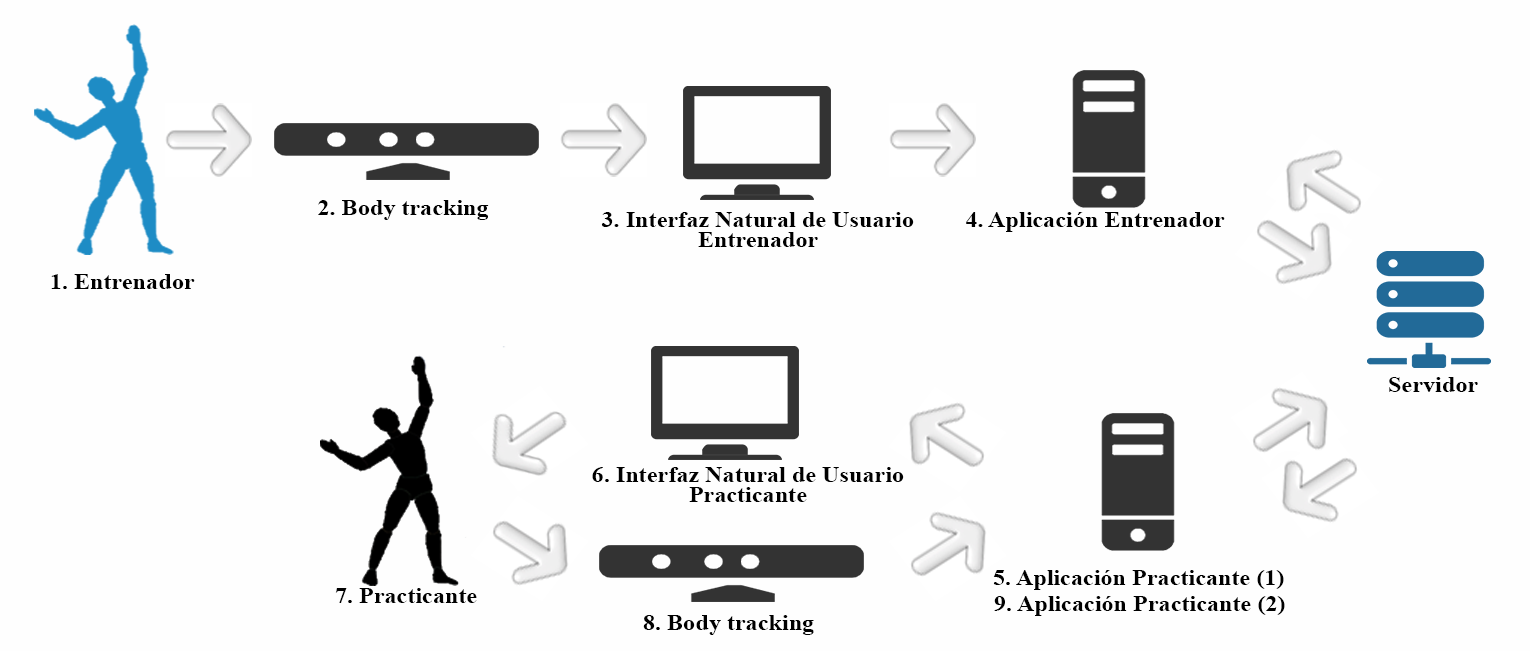
\includegraphics[scale=0.35]{./Figuras/DiagramaBloques}
	\end{center}
	\caption{Diagrama a bloques del diseño de la herramienta}
	\label{fig:Bloques}
\end{figure}

Proceso de la solución propuesta:

\begin{enumerate}
	\item \textbf{Entrenador.} Usuario especializado en Karate Do que registra los movimientos de la rutina de entrenamiento, además lleva un seguimiento del desempeño de los Practicantes. 
	\item \textbf{Body tracking.} El sensor Kinect realiza el seguimiento de los puntos del cuerpo del usuario los cuales son utilizados en la Interfaz Natural De Usuario Entrenador y en la Aplicación Entrenador. 
	\item \textbf{Interfaz Natural de Usuario Entrenador.} La interfaz con la que será mostrada y controlada la etapa de captura de movimientos de la interacción con los puntos obtenidos previamente por el sensor Kinect. 
	\item \textbf{Aplicación Entrenador.} 
	Con la información del body tracking obtenida por el sensor Kinect se realizará la captura de ejercicios y movimientos que el usuario Entrenador indique, teniendo en la aplicación un apartado con la gestión rutinas así como la gestión de los resultados de sus practicantes. 
	\item \textbf{Aplicación Practicante (1).} Recibe la información enviada por la aplicación Entrenador. 
	\item \textbf{Interfaz Natural de Usuario Practicante.} La interfaz con la que será mostrada y controlada la etapa de captura y validación de movimientos de interacción; además de mostrar los movimientos recibidos en la aplicación Entrenador. 
	\item \textbf{Practicante.} Usuario aprendiz en el entrenamiento del Karate Do quien recreará los movimientos de la rutina recibida del Entrenador. 
	\item \textbf{Body tracking.} El sensor Kinect realiza el seguimiento de los puntos del cuerpo del usuario los cuales son utilizados en la Aplicación Practicante. 
	\item \textbf{Aplicación Practicante (2).} Con la información del body tracking obtenida por el sensor Kinect se realiza la captura de ejercicios y movimientos del usuario Practicante, los cuales serán comparados con los movimientos recibidos realizados por el Entrenador, dando el resultado de su desempeño, mostrándolo en la Interfaz Natural de Usuario Practicante y enviándolo a través de internet a la aplicación Entrenador.
\end{enumerate}
%------------------------------------------------------------------------------------
\section{Objetivos}
\subsection{General}

Desarrollar una herramienta de software para el entrenamiento asíncrono a distancia (ver sección \ref{sec:elearning} \nameref{sec:elearning}) de la técnica inicial de cinta blanca de Karate Do (ver sección \ref{sec:Karate-Do} \nameref{sec:Karate-Do}), mediante el uso del sensor Kinect para el análisis de movimientos y para brindar apoyo en el seguimiento del desempeño del Practicante por parte del Entrenador.

\subsection{Específicos}
\begin{itemize}
	\item Delimitar los ejercicios de calentamiento de acuerdo a un organismo oficial.
	\item Delimitar los movimientos de la técnica inicial de cinta blanca de Karate Do.
	\item Definir los gestos y medios utilizados por el usuario para controlar la herramienta.
	\item Identificar y capturar  los movimientos del usuario.
	\item Implementar un mecanismo para la validación de movimientos.
	\item Implementar un medio de comunicación entre las aplicaciones de Entrenador y Practicante.
\end{itemize}
%------------------------------------------------------------------------------------
\section{Justificación}
Las estadísticas del INEGI reflejan el poco interés de los  mexicanos por realizar alguno de los que deportes que se ofertan, ya que de acuerdo a cifras recientes en ``deporte y ejercicio"  la tasa de participación en alguna actividad física-deportiva es de 43.8\%,  pero sólo el 30\% de la población lo práctica de manera regular o disciplinada, quienes en promedio invierten 3 horas 57 minutos a la semana \cite{INEGI}. Adicionalmente tomando como ejemplos las situaciones que se viven en otros países, como es el caso de España en el cual encuestas revelan que el principal resultado sobre la causa ó motivo por el cual las personas abandonaron algún deporte, fue el traslape de tiempos con sus actividades, sin embargo tenían en promedio 2-3 horas libres que les gustaría emplear practicando alguna actividad físico-deportiva. Los resultados también muestran que el aspecto que más influye o ayudaría para volver a practicar alguna actividad físico-deportiva es ``tener un monitor o Entrenador bien preparado" \cite{Efdeportes}.\\

Retomando la situación de nuestro país, con respecto a la elección del lugar donde se practica deporte, 49\% de los encuestados manifestaron que está relacionada sobre todo con la cercanía, un 17\% considera que lo ha elegido dado que cuenta con entrenadores confiables y un 14\% con el hecho de que se paga un precio accesible \cite{UVM}. Estos resultados muestran que se podría impulsar a las personas proporcionándoles los medios para que practiquen o continúen la actividad físico-deportiva de su agrado.\\

Existen aplicaciones comerciales que fomentan las actividades físico-deportivas, que permiten a los usuarios realizar una serie de rutinas programadas donde solamente se validan los movimientos de la rutina y se da un puntaje en base al desempeño, sin llegar a ser una disciplina formal, y en la mayoría de los casos no teniendo en cuenta la salud del usuario, al no realizar ejercicios previos de calentamiento.\\

En base a estas observaciones se ha determinado que a las personas les sería útil una aplicación donde un Entrenador dé indicaciones y pueda monitorear el desempeño del Practicante, pues el Entrenador es el experto que conoce los ejercicios que está enseñando. Una característica adicional de la aplicación que se plantea desarrollar es la retroalimentación profesor-alumno de los errores cometidos por el Practicante, dando instrucciones  de corrección y/o sugerencia.\\

Debido a que se hará la captura de movimientos de un Entrenador, y por medio de la interfaz natural de usuario, el estudiante replicará los movimientos; es posible que cualquier institución adopte este sistema, pero en el presente trabajo terminal se ha delimitado al entrenamiento de la técnica del Karate Do.
\chapter{Marco teórico}
En el presente capítulo se realiza la investigación correspondiente al estado del arte y marco teórico, comenzando con el trabajo previo el cuál está dividido en: productos de investigación, trabajos terminales y productos comerciales. La descripción de las principales herramientas de apoyo, definiciones y 
conceptos utilizados en este trabajo terminal.

%------------------------------------------------------------------------------------
\section{Estado del arte}
Por medio de una investigación realizada, en la que se buscaron trabajos con propuestas similares a la nuestra, se encontró que dentro de ESCOM no existen trabajos que aborden nuestra propuesta, sin embargo se encuentran considerados algunos de ellos por contar con validaciones de movimientos; para el caso de investigaciones científicas, se tienen diferentes trabajos similares en el aspecto de que tienen el Karate Do como base y realizan una validación de movimientos de su técnica y apoyo al entrenamiento del mismo, así como de un trabajo en el que se realiza una validación de posiciones específicas que no son comúnmente detectadas en otros trabajos; y por último se consideraron algunos productos comerciales (videojuegos) que proponen una activación física al usuario y que por medio de una validación de movimientos reflejan un resultado de su desempeño en comparación con los movimientos programados dentro de la aplicación. Sin embargo, ningún trabajo encontrado plantea el concepto de un entrenamiento deportivo formal a distancia.\\

\begin{table}[H]
\centering
\begin{tabular}{| p{4 cm} | p{7 cm} | p{4 cm} |}
\hline
\multicolumn{3}{| >{\columncolor[rgb]{0.529412, 0.807843, 0.980392}} c |} {\textbf{Productos de investigación}}\\
\hline
\rowcolor[rgb]{0.529412, 0.807843, 0.980392} \hspace{3em}{\textbf{Software}} & \hspace{5em}{\textbf{Características}} & \hspace{2em}{\textbf{Publicación}}\\
\hline
Game based approach to learn Martial Art for beginners \cite{Chye} & Primera parte de una investigación en la cual se desarrolla un videojuego con el objetivo de que los usuarios aprendan un arte Marcial (Thai boxing). A través de puntos del cuerpo, utilizando algoritmos del análisis de la postura (distancia euclidiana).

En este artículo, se enfocan en la precisión de las mediciones de las partes del cuerpo humano (estimación de altura). & 2012 IEEE International Conference on Embedded and Real-Time Computing Systems and Applications.\\
\hline
In Search of a Usability of Kinect in the Training of Traditional Japanese ``KATA"\-Stylized Gestures and Movements \cite{Wada} & Proponen un sistema para el entrenamiento de ``KATAS", en este artículo se desarrolla una parte del sistema que obtiene coordenadas tridimensionales en 20 diferentes puntos de las articulaciones del cuerpo humano y es capaz de medir los ángulos en algunas posiciones. & IEEE 2013.\\
\hline
Computer Karate Trainer in Tasks of Personal and Homeland Security Defense \cite{Hachaj} & Se presenta una nueva posibilidad de utilizar lenguajes de descripción de gestos (GDL por sus siglas en inglés) para el reconocimiento de técnicas básicas de las artes marciales.  El enfoque del GDL permite no sólo analizar varias técnicas del Karate Shorin-Ryu sino que permite apoyar al entrenamiento y la enseñanza de dichas artes. & IFIP International Federation for Information Processing 2013.\\
\hline
Safe Lifting: An adaptive Training System for Factory Workers Using the Microsoft Kinect \cite{Delpresto} & Es un proyecto de investigación el cual tiene como objetivo el diseñar un sistema de monitoreo preciso que pueda ayudar a trabajadores de fábricas a corregir sus técnicas de levantamiento pesado por medio de recomendaciones de técnicas adaptativas. Apoyándose en el uso de la cámara de profundidad del sensor Kinect y definiendo las técnicas de levantamiento usando varias ecuaciones de levantamiento y varios modelos biomecánicos. & Proceedings of the 2013 IEEE Systems and Information Engineering Design Symposium, University of Virginia 2013.\\
\hline
\end{tabular}
\caption{Productos de investigación}
\end{table}

\begin{table}[H]
\centering
\begin{tabular}{| p{4 cm} | p{8 cm}| p{3 cm} |}
\hline
\multicolumn{3}{| >{\columncolor[rgb]{0.529412, 0.807843, 0.980392}} c|} {\textbf{Trabajo Terminal}}\\
\hline
\rowcolor[rgb]{0.529412, 0.807843, 0.980392} \hspace{4em}{\textbf{Software}} & \hspace{5em}{\textbf{Características}} & {\textbf{Precio en el mercado}}\\
\hline
TT2013-A015 Sistema de apoyo para el tratamiento del sobrepeso y obesidad infantil utilizando el sensor Kinect. & Este proyecto consiste en desarrollar una herramienta que permita llevar un seguimiento y control de rutinas de ejercicios físicos para un infante. El sistema le asignará una serie de ejercicios que el usuario deberá realizar y por medio del sensor Kinect se captarán los movimientos que va ejecutando, asimismo podrá conocer el registro de las actividades físicas que ha estado realizando. & No aplica\\
\hline
TT2012-B007 Control de movimientos de un robot vía Kinect & Sistema de transferencia de movimientos o habilidades, mediante una interfaz de natural de usuario (NUI, por sus siglas en inglés) con ayuda del sensor Kinect, la cual permite analizar el movimiento del cuerpo, y de esta manera dar instrucciones precisas al robot para que imite un movimiento. & No aplica\\
\hline
\multicolumn{3}{| >{\columncolor[rgb]{0.529412, 0.807843, 0.980392}} c|} {\textbf{Productos comerciales}}\\
\hline
Nike+ Kinect Training & Sea cual sea tu nivel, sea cual sea tu objetivo, con Nike+ Kinect Training podrás tener un entrenamiento personal en casa. Usando retroalimentación en tiempo real como en una sesión profesional, podrás elegir un programa que irá evolucionando según tus progresos. Esto es Nike+ Kinect Training para Xbox 360. & \$499\\
\hline
Dance central 3 & El juego consiste en representar los movimientos de baile que el personaje en pantalla va realizando. A la derecha tenemos los movimientos que estamos realizando, su nombre, y los que vendrán a continuación. Dance Central está pensado para aprender a bailar y representar los movimientos, muchos de ellos complicados de encadenar al principio, a la perfección. & \$299\\
\hline
\end{tabular}
\caption{Trabajos Terminales y Productos comerciales}
\end{table}
%------------------------------------------------------------------------------------
\section{Sensor Kinect}
\subsection{Historia}
El primer anuncio de Kinect fue el 1 de Junio de 2009 en la E3 2009 bajo el nombre de ``Project Natal".\\

Kinect es una línea de dispositivos de detección de movimientos de Microsoft para las consolas de videojuegos Xbox 360 así como para PCs con sistema operativo Windows. Basado en torno a un periférico tipo webcam, permite a los usuarios controlar e interactuar con su consola/computadora sin la necesidad de un control de juego, a través de una interfaz natural de usuario usando gestos y comando de voz \cite{Microsoft2}.\\

Formalmente Microsoft presentó en Junio del 2010 en la E3 que su sistema se llamaría oficialmente Kinect \cite{Snider}.
%------------------------------------------------------------------------------------
\subsection{Descripción del hardware}
El Kinect se compone de una cabeza y de una base, como se muestra en la Figura \ref{fig:Kinect}. La cabeza es de 12 x 2.5 x 1.5 pulgadas. La unión entre la base y la cabeza está motorizada. El dispositivo físico contiene cámaras, una colección de micrófonos y un acelerómetro \cite{Webb}.

\begin{figure}[h]%La h significa que la colocara cerca del texto
	\begin{center}
		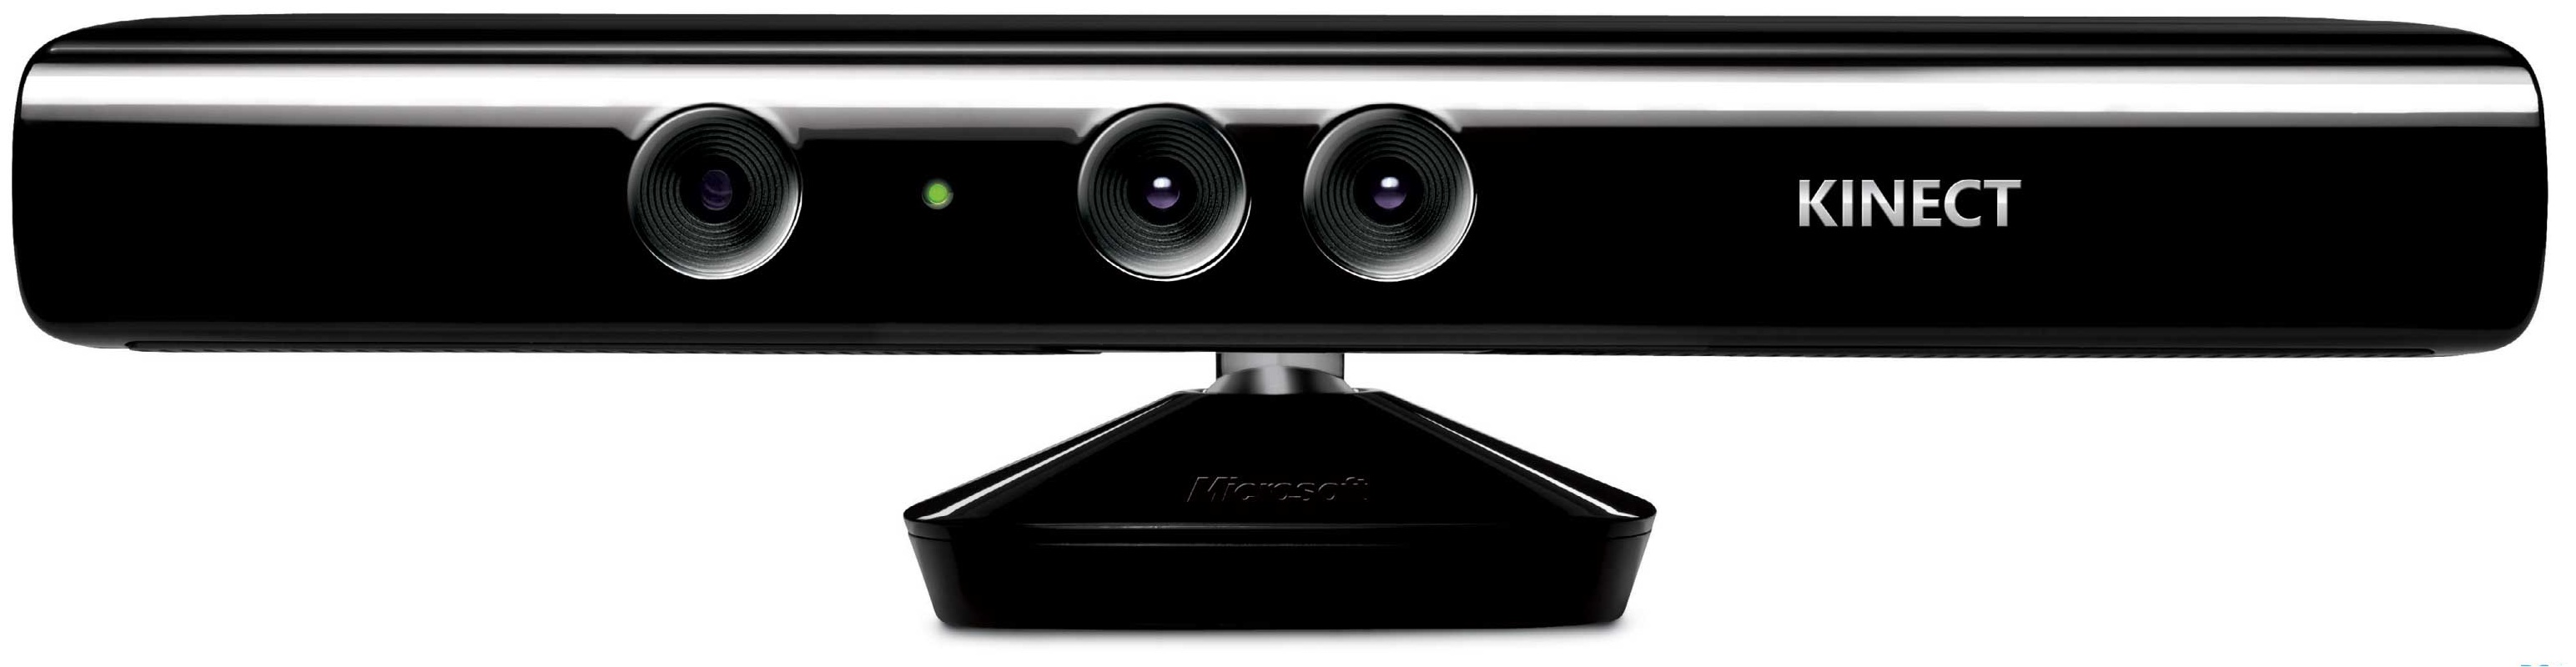
\includegraphics[scale=0.15]{./Figuras/KinectFrontal}
	\end{center}
	\caption{Vista frontal del Kinect}
	\label{fig:Kinect}
\end{figure}

Dentro del recubrimiento del sensor, un Kinect para Windows contiene:

\begin{itemize}
\item Una cámara RGB que almacena 3 canales de datos en una resolución de 1280x960. Esto permite capturar imágenes a color.
\item Un emisor infrarrojo (IR) y un sensor infrarrojo de profundidad. El emisor emite destellos de luz infrarroja y el sensor de profundidad lee los haces de luz infrarroja reflejadas de nuevo al sensor. Los haces reflejados son convertidos en información de profundidad midiendo la distancia entre un objeto y el sensor. Esto permite capturar la profundidad de una imagen.
\item Un micrófono multi-array, el cual contiene 4 micrófonos para capturar sonido. Debido a los 4 micrófonos, es posible grabar audio, así como encontrar la ubicación de la fuente de sonido y la dirección de la onda de audio.
\item Un acelerómetro de 3 ejes configurado para rango 2G donde la G es la aceleración debida a la gravedad. Es posible usar el acelerómetro para determinar la orientación actual del Kinect \cite{Microsoft3}.
\end{itemize}

\begin{figure}[h]%La h significa que la colocara cerca del texto
	\begin{center}
		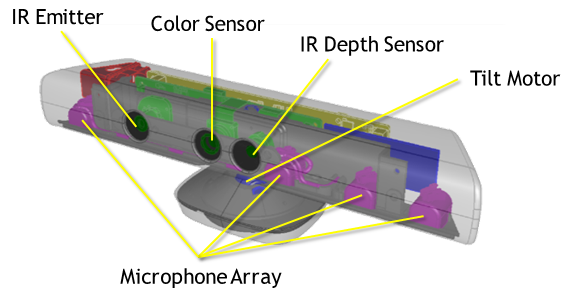
\includegraphics[scale=1]{./Figuras/KinectHardware}
	\end{center}
	\caption{Hardware interno del Kinect}
	\label{fig:KinectHardware}
\end{figure}
%------------------------------------------------------------------------------------
\subsection{Kinect SDK}
Microsoft Kinect SDK, provee las herramientas y API's necesarias para desarrollar aplicaciones para Microsoft Windows usando la tecnología de sensores de Kinect \cite{MicrosoftSDK}.\\

Existen 4 actualizaciones de la versión de SDK para el sensor Kinect, de las cuales la 1.8 es la versión a utilizar en el presente trabajo terminal, algunas características que se tienen hasta el momento son:
\begin{itemize}
\item Kinect Studio: Herramienta que permite a los desarrolladores grabar y reproducir datos de Kinect.
\item Reconocimiento del esqueleto ``sentado": Permite el seguimiento de 10 puntos (cabeza, cuello y brazos) ignorando las piernas y la cintura.
\item Datos ampliados profundidad: Las aplicaciones serán capaces de leer los datos más allá de cuatro metros cuando sea necesario.                                                                                                                  
\item APIs de configuración de la cámara a color: Los ajustes de la cámara de color se pueden optimizar para su entorno.
\item Nueva API de conversión de coordenadas espacio: Hay dos conjuntos de APIs, uno para la conversión de los píxeles individuales y la otra para la conversión de un cuadro de imagen completa.
\item Kinect Interactions: Ofrece la posibilidad a los desarrolladores de crear aplicaciones intuitivas que utilicen los gestos más comunes de la gente.
\item Kinect for Windows Interactions: Transforma la manera en la que la gente se comunica con la computadora.
\item Incluye herramientas de desarrollo mejoradas y más recursos para los desarrolladores tales como: Ejemplos de OpenCV y MATLAB compatibles con Kinect, ejemplos de código de Kinect para Windows para CodePlex ofreciendo la posibilidad de desarrollar en una plataforma open-source \cite{Heddle1}.
\end{itemize} 

Las características principales de la última versión (1.8) incluyen: 
\begin{itemize}
\item Un nuevo efecto de pantalla verde: Permite borrar el fondo detrás del usuario activo y después intercambiarlo por un fondo artificial.
\item Capacidades mejoradas para modelado en 3D: Permiten escanear el color de una escena al igual que sus contornos, lo que hace posible la impresión de objetos en 3D a todo color o pueda agregarse fidelidad a las características de los juegos y otras aplicaciones.
\item Una muestra de interfaz de usuario adaptable: Muestra cómo construir una aplicación que se adapta de acuerdo con la distancia entre el usuario y la pantalla para detección de gestos y tacto \cite{Heddle2}.
\end{itemize}
%------------------------------------------------------------------------------------
\subsection{Kinect SDK Open Source}
\subsubsection{OpenNI (Open Natural Interaction)}
Es un framework de código abierto creado por la empresa PrimeSense, permite comunicarse con los sensores de audio, video y sensor de profundidad de Kinect, mientras que proporciona una API que sirve de puente entre el hardware del equipo, NITE Middleware y las aplicaciones e interfaces del Sistema Operativo.  Su idea es facilitar el desarrollo de aplicaciones que funcionen con interacción natural, como gestos y movimientos corporales \cite{Echeverria}. \\

En noviembre del 2013, Apple compró la empresa PrimeSense. El 23 de abril del 2014, la página de OpenNI cerró y la descarga del software quedó deshabilitada desde esa fecha \cite{Armstrong}.

\subsubsection{OpenKinect}
Su objetivo principal actualmente es el software libfreenect, éste incluye todo el código necesario para activar, inicializar y comunicar los datos con el hardware de Kinect. La API  tiene enlaces y extensiones para los siguientes idiomas y plataformas: C, C++, NET (C\#), Java, Python, C y la interfaz síncrona.\\

OpenKinect también tiene como proyecto, la librería de análisis la cual se comunica con el API y analiza la información en bruto en abstracciones más útiles; así como aplicaciones, que incluyan códigos de ejemplo, demos, o cualquier aplicación que los usuarios quieran compartir.\\

El usuario que contribuya, puede optar por utilizar el proyecto con la licencia Apache 2.0 o licencia GPL v2 \cite{OpenKinect}. 
%------------------------------------------------------------------------------------
\section{Interfaz Natural de Usuario (INU)}

Existen diferentes definiciones de Interfaz natural de usuario tal como lo puntualizan los siguientes autores: \\

Una Interfaz natural de usuario es una interfaz de usuario diseñada para reutilizar habilidades existentes para interactuar directamente con contenido. ``Interfaz natural de usuario es la nueva forma de pensamiento acerca de como podemos interactuar con dispositivos de computación" \cite{Blake}. \\

La Interfaz natural de usuario (INU) es una evolución de la interfaz gráfica de usuario (GUI) y surge como un mecanismo de interacción hombre-máquina que permite establecer una  comunicación con sistemas computacionales a través de periféricos que pueden recibir instrucciones e información. La INU tiene algunas consideraciones adicionales las cuales se enfocan en hacer uso de una comunicación de manera natural con el ser humano, haciendo uso del captar información en tiempo real logrando una interacción corporal de manera directa, sin utilizar un periférico que actúe como intermediario para la entrada de información \cite{Gomez}. \\

La INU fundamenta sus principios en lo siguiente: debe ser directo, intuitivo e invisible al usuario (o hacerse invisible por medio de interacciones sencillas explicadas al usuario). No tiene que ser aprendido, porque está basado en elementos naturales, es decir, en los comandos utilizados en los comportamientos humanos habituales. Integra armoniosamente un balance entre fisiología y kinesiología, creando una interfaz para dedos vivos, no para cursores \cite{Sarajevo}. \\

\textbf{¿Qué significa natural?} \\

Una interfaz natural es aquella que ``explota las habilidades que hemos adquirido a través del tiempo vivido en el mundo" \cite{Buxton}. \\

La descripción anterior es interesante por dos razones. Primero, relaciona el concepto natural con la idea de rehusar habilidades existentes. Segundo, hace explícito que estas habilidades no son solamente habilidades innatas con las cuales nacimos. Natural significa usar habilidades innatas mas habilidades aprendidas y que hemos desarrollado a través de la interacción con nuestro propio ambiente natural cada día de la vida. \\

\textbf{¿Qué es una habilidad simple?} \\

Las habilidades simples solo dependen de las habilidades innatas aprendidas. Esto limita su complejidad, lo que también significa que son fáciles de aprender, tienen una baja carga cognitiva, y pueden ser rehusadas y adaptadas para muchos objetivo sin mucho esfuerzo. El proceso de aprendizaje de habilidades simples es típicamente muy veloz y requiere poca o ninguna práctica para alcanzar un adecuado nivel de competencia. En muchas ocasiones, este aprendizaje se puede alcanzar simplemente observando a alguien mas demonstrar la habilidad una o dos veces \cite{Blake}.

\subsection{Características de una Interfaz natural de usuario} 

\textbf{Centrada en el usuario} \\

Se toman como partida las necesidades cambiantes de la interfaz de usuario, de manera que se modifica la interfaz de usuario de la forma externa y los mecanismos internos para satisfacer las necesidades de los diferentes usuarios, lo cual es llamado diseño centrado en el usuario. La tecnología de reconocimiento de voz no específica de discursos humanos permitirá a las computadoras comprender las demandas de las personas, esta es una interfaz de entrada importante. \\

La tecnología fisheye observa la posición de los alrededores de un contenido con respecto a una posición en la pantalla, la cual es aumentada y es llamada observación amigable del usuario. En los sistemas tradicionales humano-maquina, las personas son consideradas como los operadores, es decir, personas que se adaptan a la máquina; en los sistemas generales hombre-máquina, las personas son conocidas como usuarios, pueden dialogar con la máquina, pero no tienen el control activo; en los sistemas de realidad virtual, las personas son participantes activos, donde la máquina responderá a diferentes acciones humanas. \\

\textbf{Multicanal} \\

Las interfaces multicanal tienen la intención de hacer un uso completo de uno o más de los canales sensores y motores, para capturar las características complementarias de los propósitos de los usuarios, para mejorar la naturalidad de la interacción hombre-máquina. \\

Los sentidos sensoriales humanos son la visión, el oído, el tacto, el olfato y el gusto; los canales de gestos humanos son las manos, la boca, los ojos, la cabeza, los pies, el cuerpo y así sucesivamente. Ahora, para las operaciones computacionales, los ojos humanos y las manos están muy cansados y la eficiencia no es alta \cite{Weiyuan}. Si escuchamos a, por ejemplo, la coordinación mano-ojo y otras acciones multicanal, se puede lograr una interacción natural y una comunicación humano-máquina eficiente así como brindar la posibilidad de elegir el mejor canal de respuesta posible, de tal manera que no se haga una sobrecarga sobre dichos canales. \\

\textbf{Inexacta} \\

La tecnología interactiva precisa, es una tecnología que puede ser usada para explicar completamente el propósito de las interacciones del usuario. El teclado y el ratón son necesarios para ingresar datos con precisión, pero las acciones de las personas o pensamientos no son muy precisos. Las computadores deben entender las peticiones de las personas e incluso corregir sus errores. Una interfaz que sea inteligente es una orientación importante. \\

\textbf{Alto ancho de banda} \\

Ahora las salidas de una computadora tienen que ser rápidas, con un continuo despliegue de imágenes a color y de una gran cantidad de información. Pero las personas aún utilizan como entrada el teclado en una que otra ocasión, por lo cual el ancho de banda es muy bajo. Las Interfaces naturales de usuario deben soportar un ancho de banda de entrada alto y una rápida importación de grandes cantidades de información. La entrada y entendimiento de voz, imagen, y la postura es una orientación de desarrollo para la actualidad y el futuro. \\

\textbf{Interacciones basadas en voz} \\

El lenguaje ha sido reconocido por mucho tiempo como el flujo más natural, conveniente y eficiente para el intercambio de información. En la vida diaria la comunicación humana es en un 75\% ejecutada por voz \cite{Weiyuan}. Los resultados muestran que existen muchas ventajas sobre los canales auditivos, como que la detección de canales auditivos es más rápida que la velocidad de detección de señales visuales. El cambio de un sonido personal es extremadamente sensible; la información auditiva y visual puede proporcionar el acceso a más personas hacia la existencia de un fuerte sentido de realismo, etc. Por lo tanto, el canal auditivo es el mas importante canal de interacción entre una computadora y otro dispositivo de información \cite{Weiyuan}. \\

La interacción por voz es una interacción con tecnología computacional para estudiar el como las personas interactúan a través de voz o voz sintetizadas por máquina. Esto involucra diferentes disciplinas como lingüística, psicología, ergonomía y tecnologías de la computación; al mismo tiempo es una visión hacía el futuro dirigido a la interacción por voz, su diseño y desarrollo. \\

Los sistemas interactivos por voz típicamente toman dos aproximaciones: una es basada en una tecnología de reconocimiento y entendimiento, que depende principalmente del sistema de audio con el que se interactúa; el otro es el uso de una tecnología de voz y de sistemas combinados en otras formas para interactuar con el sistema. De esta forma, la voz ya no es dominante sino sólo una parte de un sistema interactivo. \\

\textbf{Interacción basada en imagen} \\

La interacción por imagen simplemente es una computadora basada en comportamiento humano que entiende una imagen y entonces reacciona. \\

En el presente, los sistemas de visión artificial se pueden dividir en 3 niveles: el procesamiento de imagen (al más bajo nivel), el reconocimiento de imágenes (a un alto nivel) y la percepción de imágenes (al más alto nivel). El procesamiento de imágenes es el proceso de ingresar una imagen como entrada y de tener una imagen a la salida \cite{Weiyuan}. El reconocimiento de patrones, se interesa principalmente en la detección de objetivos en la imagen y su medición, para obtener información objetiva, con el fin de establecer la descripción de la imagen. Esencialmente es el proceso de llevar una imagen a datos. \\

La percepción de imagen se centra en estudiar aún más la naturaleza de la imagen de destino y sus relaciones mutuas sobre la base del reconocimiento de imágenes, y viene para entender el significado del contenido de una imagen e interpretación de la escena original. En la percepción de imágenes, la entrada es una imagen y la salida es una interpretación de dicha imagen. \\

\textbf{Interacciones basadas en comportamiento} \\

En el proceso de intercambio, en adición a la interacción por voz, las personas frecuentemente utilizan el lenguaje corporal, el cual involucra movimientos del cuerpo para expresar su actitud y significado, por lo tanto, es un proceso basado en interacciones humanas. El método de interacciones por acciones humanas puede no solamente mejorar las habilidades de lenguajes, sino también, puede jugar el rol de interacción que la voz no puede. \\

El comportamiento de la interacción humano-computadora es el reconocimiento de comportamiento humano a través de posicionamiento, seguimiento, movimiento y expresión de las partes del cuerpo para entender las acciones y el comportamiento, y responder con un proceso inteligente de retroalimentación. \\

Las interacciones basadas en comportamiento brindan una nueva forma de interacción. El comportamiento del usuario puede ser predecido por la computadora y así conocer las necesidades de los usuarios. Por ejemplo: con un seguimiento de la atención de las personas, se puede determinar la intención de los usuarios para visitar un sitio web especifico o la necesidad de una llamada; cuando el usuario entra en una habitación, la computadora responde enviándole un correo electrónico, si el usuario niega con la cabeza, el equipo considera que el usuario no desea leer el mensaje.
%------------------------------------------------------------------------------------
\section{Karate Do}
\label{sec:Karate-Do}
El Karate Do, en todas sus diferentes formas, encuentra sus orígenes en un sólo lugar, las islas Ryukyu fuera de la costa de Japón. Lo que se sabe de uno de los sistemas de entrenamiento de auto defensa y disciplina más practicados en el mundo es el resultado de siglos de desarrollo. \\

El Karate Do es un arte marcial tradicional en el que se coordina la fuerza, la respiración, el equilibrio y la postura, el correcto giro de cadera y la conexión conjunta de músculos y extremidades, trasladando gran parte del peso corporal y del centro de gravedad al impacto. Se caracteriza por el empleo de golpes de puño y patadas, aunque no restringe su repertorio sólo a ellos. Normalmente, un entrenamiento de Karate Do se divide en 5 partes que son: el calentamiento, los ejercicios de resistencia, la técnica, las Katas y el Kumite (o combate); el presente trabajo está enfocado en el aprendizaje de la técnica del Karate Do, por lo que se verán contemplados los ejercicios de calentamiento y los movimientos de técnica. \\

En la actualidad existen diferentes estilos en la enseñanza del Karate Do, todos basados en la técnica original, pero normalmente cambiando los métodos de enseñanza dependiendo de las regiones o incluso de cada instructor. Para el caso del presente trabajo terminal, se tiene el apoyo y asesoría del experto Moisés Gachúz Mendoza cuyo grado es de Cinta Negra 5to Dan registrado en la Federación Mexicana de Karate Do desde el 2005.
%------------------------------------------------------------------------------------
\subsection{Calentamiento}
\label{sec:Calentamiento}
El calentamiento es un aspecto importante para cualquier rutina de ejercicios. Realizar ejercicios de calentamiento antes de estiramientos, calienta la temperatura del cuerpo, lo cual incrementa el flujo de sangre en los músculos y los hace más flexibles. El calentamiento también protege al corazón, ya que las personas que calientan por al menos dos minutos antes de una rutina de ejercicios reducen su riesgo de alta presión sanguínea e incrementa el flujo de oxígeno en el corazón. El calentamiento debe ser la primera actividad realizada antes de hacer estiramientos, ejercicio cardiovascular o entrenamiento de resistencia \cite{Nall}.\\

Existen ejercicios de calentamiento recomendados especialmente para cada tipo de actividad física o deportiva, el Karate Do es un deporte que no se enfoca en una sola actividad, sino que tiene una combinación de varias, como los ejercicios de resistencia, el estiramiento o los ejercicios cardiovasculares; es por ello que para el presente trabajo terminal se proponen rutinas de entrenamiento con los siguientes ejercicios de calentamiento, Figura \ref{fig:Musculos_Cuello} - Figura \ref{fig:Musculos_Estiramiento3}, indicados como parte del Programa Nacional de Activación Física de la CONADE \cite{CONADE}:

\clearpage

\begin{figure}[H]
	\centering
	\subfloat[Flexión lateral del cuello, izquierdo y derecho]{
		\label{fig:Cuello_Frontal}
		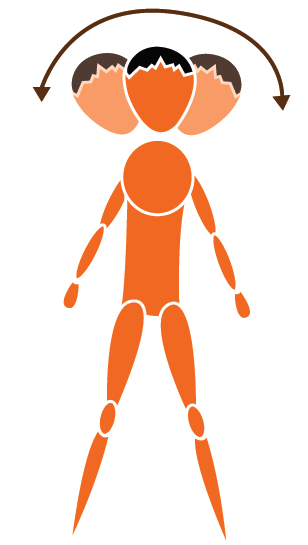
\includegraphics[width=4.5cm, height=8cm]{./Figuras/Calentamiento/1_Flexion_lateral_del_cuello}}
	\subfloat[Flexión del cuello al frente y extensión del cuello atrás]{
		\label{fig:Cuello_Lateral}
		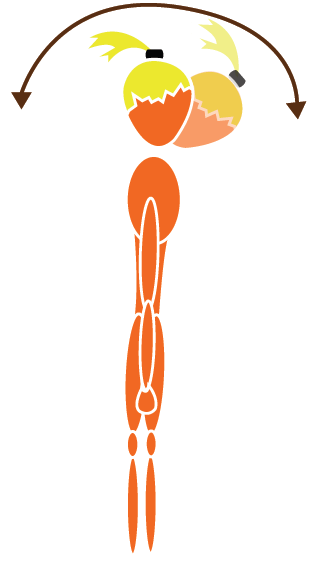
\includegraphics[width=5.5cm, height=8cm]{./Figuras/Calentamiento/2_Flexion_del_cuello_al_frente}}
	\caption{Músculos de cuello}
	\label{fig:Musculos_Cuello}
\end{figure}

\begin{figure}[H]
	\begin{center}
		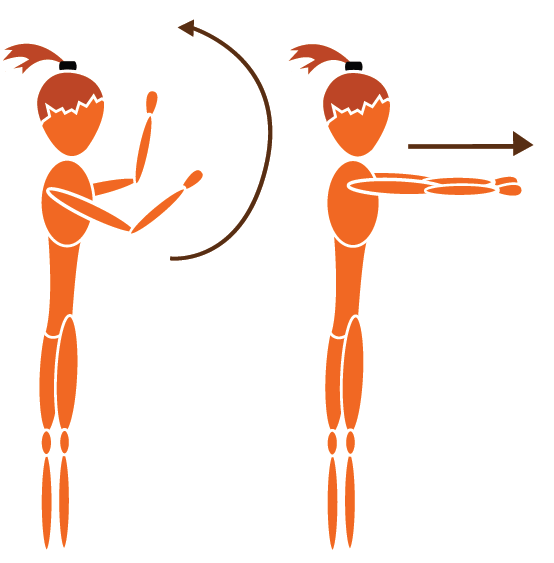
\includegraphics[width=8cm, height=8cm]{./Figuras/Calentamiento/7_Flexion_del_codo}\\
		Flexión y extensión del codo
	\end{center}
	\caption{Músculos del brazo}
	\label{fig:Musculos_Brazo}
\end{figure}

\begin{figure}[H]
	\centering
	\subfloat[Flexión y extensión del tronco(enfrente y atrás)]{
		\label{fig:Tronco_Frontal}
		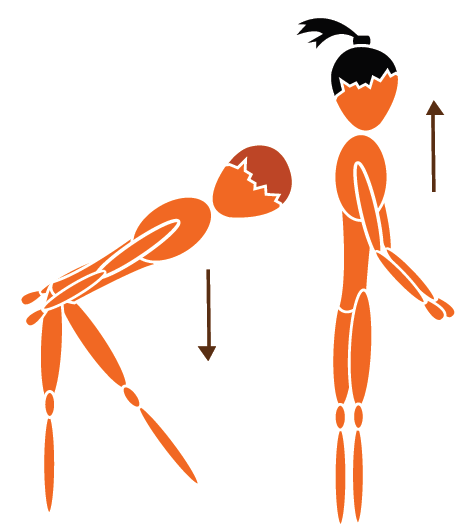
\includegraphics[width=7cm, height=8cm]{./Figuras/Calentamiento/12_Flexion_del_tronco}}
	\subfloat[Flexión del tronco izquierdo y derecho]{
		\label{fig:Tronco_Lateral}
		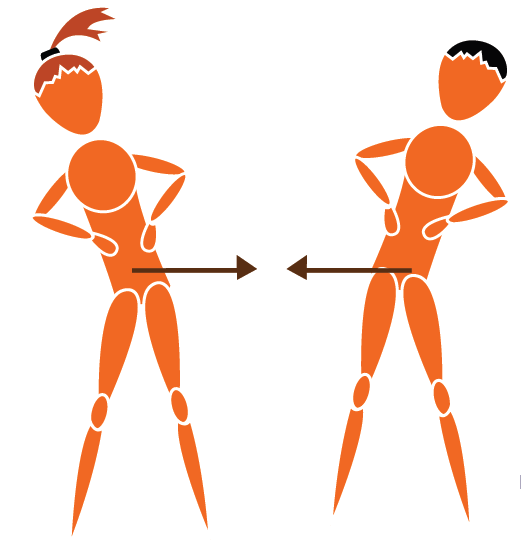
\includegraphics[width=5.5cm, height=8cm]{./Figuras/Calentamiento/13_Flexion_lateral_del_tronco}}
	\caption{Músculos de la cadera}
	\label{fig:Musculos_Cadera}
\end{figure}

\begin{figure}[H]
	\centering
	\subfloat[Flexión y extensión de rodilla]{
		\label{fig:Piernas_Frontal}
		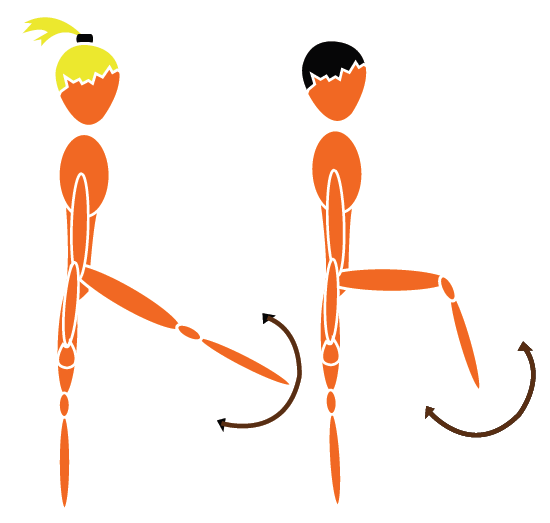
\includegraphics[width=8cm, height=8cm]{./Figuras/Calentamiento/15_Flexion_de_la_rodilla}}
	\subfloat[Abrir y cerrar las piernas derecha e izquierda]{
		\label{fig:Piernas_Lateral}
		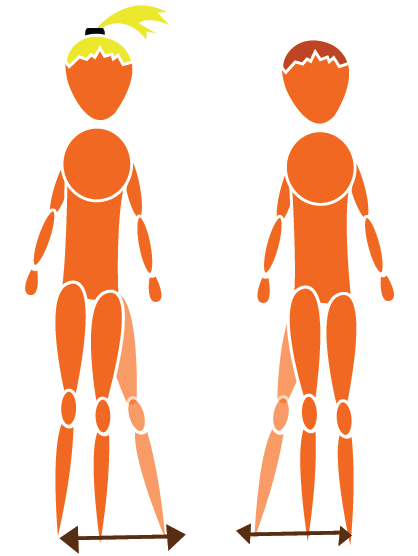
\includegraphics[width=5.5cm, height=8cm]{./Figuras/Calentamiento/16_Abrir_piernas}}
	\caption{Músculos de la pierna}
	\label{fig:Musculos_Pierna}
\end{figure}

\begin{figure}[H]
	\centering
	\subfloat[Estiramiento de músculos posteriores de la pierna]{
		\label{fig:Musculos_Estiramiento1}
		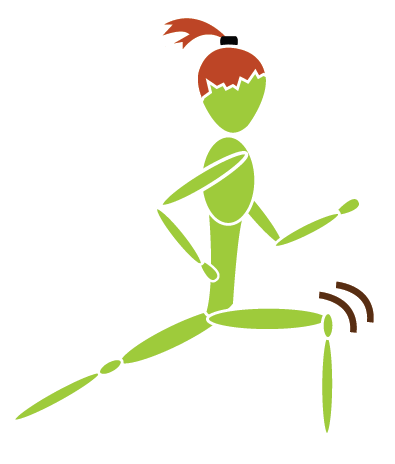
\includegraphics[width=5.5cm, height=8cm]{./Figuras/Calentamiento/28_Estiramiento_de_musculos_de_la_pierna}}
	\subfloat[Estiramiento del músculo de la pierna]{
		\label{fig:Musculos_Estiramiento2}
		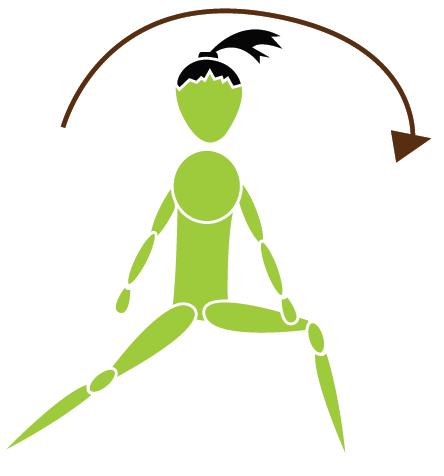
\includegraphics[width=5.5cm, height=8cm]{./Figuras/Calentamiento/29_Estiramiento_del_musculo_de_la_pierna}}
	\caption{Estiramientos de pierna}
	\label{fig:Estiramientos_Pierna}
\end{figure}

\begin{figure}[H]
	\begin{center}
		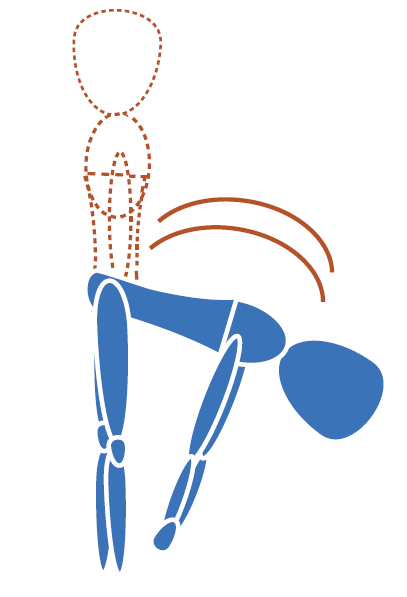
\includegraphics[width=5.5cm, height=8cm]{./Figuras/Calentamiento/44_lab_Flexion_de_tronco_al_frente}\\
		Separación de las piernas a la altura de los hombros, se flexiona el tronco tocando la punta de los pies
	\end{center}
	\caption{Estiramiento}
	\label{fig:Musculos_Estiramiento3}
\end{figure}

%-----------------------------------------------------------------------------
\subsubsection{Descripción de ejercicios}
La siguiente tabla muestra la lista de los ejercicios de calentamiento propuestos en la herramienta, describiendo la manera de realizarse y su utilidad en la realización de la técnica del Karate Do.

\begin{table}[H]
\centering
\begin{tabular}{| p{3 cm} | p{4 cm} | p{4 cm} | p{4 cm} |}
\hline
\rowcolor[rgb]{0.529412, 0.807843, 0.980392} {\textbf{Parte del cuerpo}} & {\textbf{Postura}} & {\textbf{Descripción}} & {\textbf{Técnica de Karate Do}}\\
\hline
\textbf{Calentamiento de músculos del cuello} &  Brazos extendidos a los costados.
Piernas ligeramente abiertas a la altura de los hombros. & Flexión lateral del cuello, hacia la izquierda y hacia la derecha. & Es necesario para realizar posiciones de manera precisa.\\
\hline
\textbf{Calentamiento de músculos del cuello} & Brazos extendidos a los costados.
Piernas ligeramente abiertas a la altura de los hombros. & Flexión del cuello hacia el frente y extensión del cuello hacia atrás. & Es necesario para realizar posiciones de manera precisa.\\
\hline
\textbf{Calentamiento de músculos del brazo} & Piernas ligeramente abiertas a la altura de los hombros.
Brazos levantados a la altura de los hombros. & Flexión y extensión de los codos. & Es necesario para realizar posiciones, ataques con brazo y defensas de manera precisa.\\
\hline
\textbf{Calentamiento de músculos de cadera} & Piernas separadas, superando la posición de los hombros. & Flexión y extensión del tronco, hacia enfrente y atrás. & Es necesario para realizar posiciones y ataques con pierna de manera precisa.\\		
\hline
\textbf{Calentamiento de músculos de cadera} & Piernas separadas, superando la posición de los hombros. & Flexión del tronco hacia los lados derecho e izquierdo. & Es necesario para realizar posiciones y ataques con pierna de manera precisa.\\
\hline
\textbf{Calentamiento de músculos de la pierna} & Una pierna en el suelo y la otra pierna levantada a la altura de la cadera. & Flexión y extensión de la rodilla de la pierna levantada. & Es necesario para realizar posiciones y ataques con pierna de manera precisa.\\
\hline
\textbf{Calentamiento de músculos de la pierna} & Piernas ligeramente abiertas a la altura de los hombros. & Abrir y cerrar las piernas (una a la vez) haciendo movimientos de derecha a izquierda.& Es necesario para realizar posiciones y ataques con pierna de manera precisa.\\
\hline


\end{tabular}
%\caption{Descripción de ejercicios de calentamiento}
\label{tab:DEC}
\end{table} 

\begin{table}[H]
\centering
\begin{tabular}{| p{3 cm} | p{4 cm} | p{4 cm} | p{4 cm} |}
\hline
\textbf{Estiramiento de músculos de la pierna} & Una pierna flexionada hacia el frente y la otra estirada hacia atrás. & Mantener la posición por unos segundos. & Es necesario para realizar posiciones de manera precisa, así como ataques con pierna con mayor fuerza y alcance.\\
\hline	
\textbf{Estiramiento de músculos de la pierna} & Con el cuerpo de frente se estira una pierna y la otra se flexiona. & Mantener la posición por unos segundos, recargando la mayor parte del peso sobre la pierna flexionada. & Es necesario para realizar posiciones de manera precisa, así como ataques con pierna con mayor fuerza y alcance.\\
\hline
\textbf{Estiramiento de piernas y cadera} & Piernas ligeramente separadas a la altura de los hombros. & Flexionar el tronco hacia enfrente, tocando la punta de los pies con las manos.
Mantener la posición por unos segundos. & Es necesario para realizar posiciones de manera precisa, así como ataques con pierna con mayor fuerza y alcance.\\
\hline
\end{tabular}
\caption{Descripción de ejercicios de calentamiento}
\label{tab:DEC2}
\end{table} 

%------------------------------------------------------------------------------------
\subsection{Técnica}
La técnica es un procedimiento o conjunto de reglas, normas o protocolos que tienen como objetivo obtener un resultado determinado.
Para el caso del Karate Do, la técnica hace referencia al conjunto de movimientos propios de dicho deporte, como son los ataques, las defensas, las posiciones , Katas y Kumite (combate); el presente trabajo terminal está enfocado en la técnica inicial de cinta blanca la cual contempla los primeros tres, tomando como referencia los movimientos específicos que se muestran a continuación, de la Figura \ref{fig:Posiciones1} a la Figura \ref{fig:Ataques2}:

\begin{figure}[H]
	\centering
	\subfloat[Musubi - dachi frontal]{
		\label{fig:Musubidachi_Frontal}
		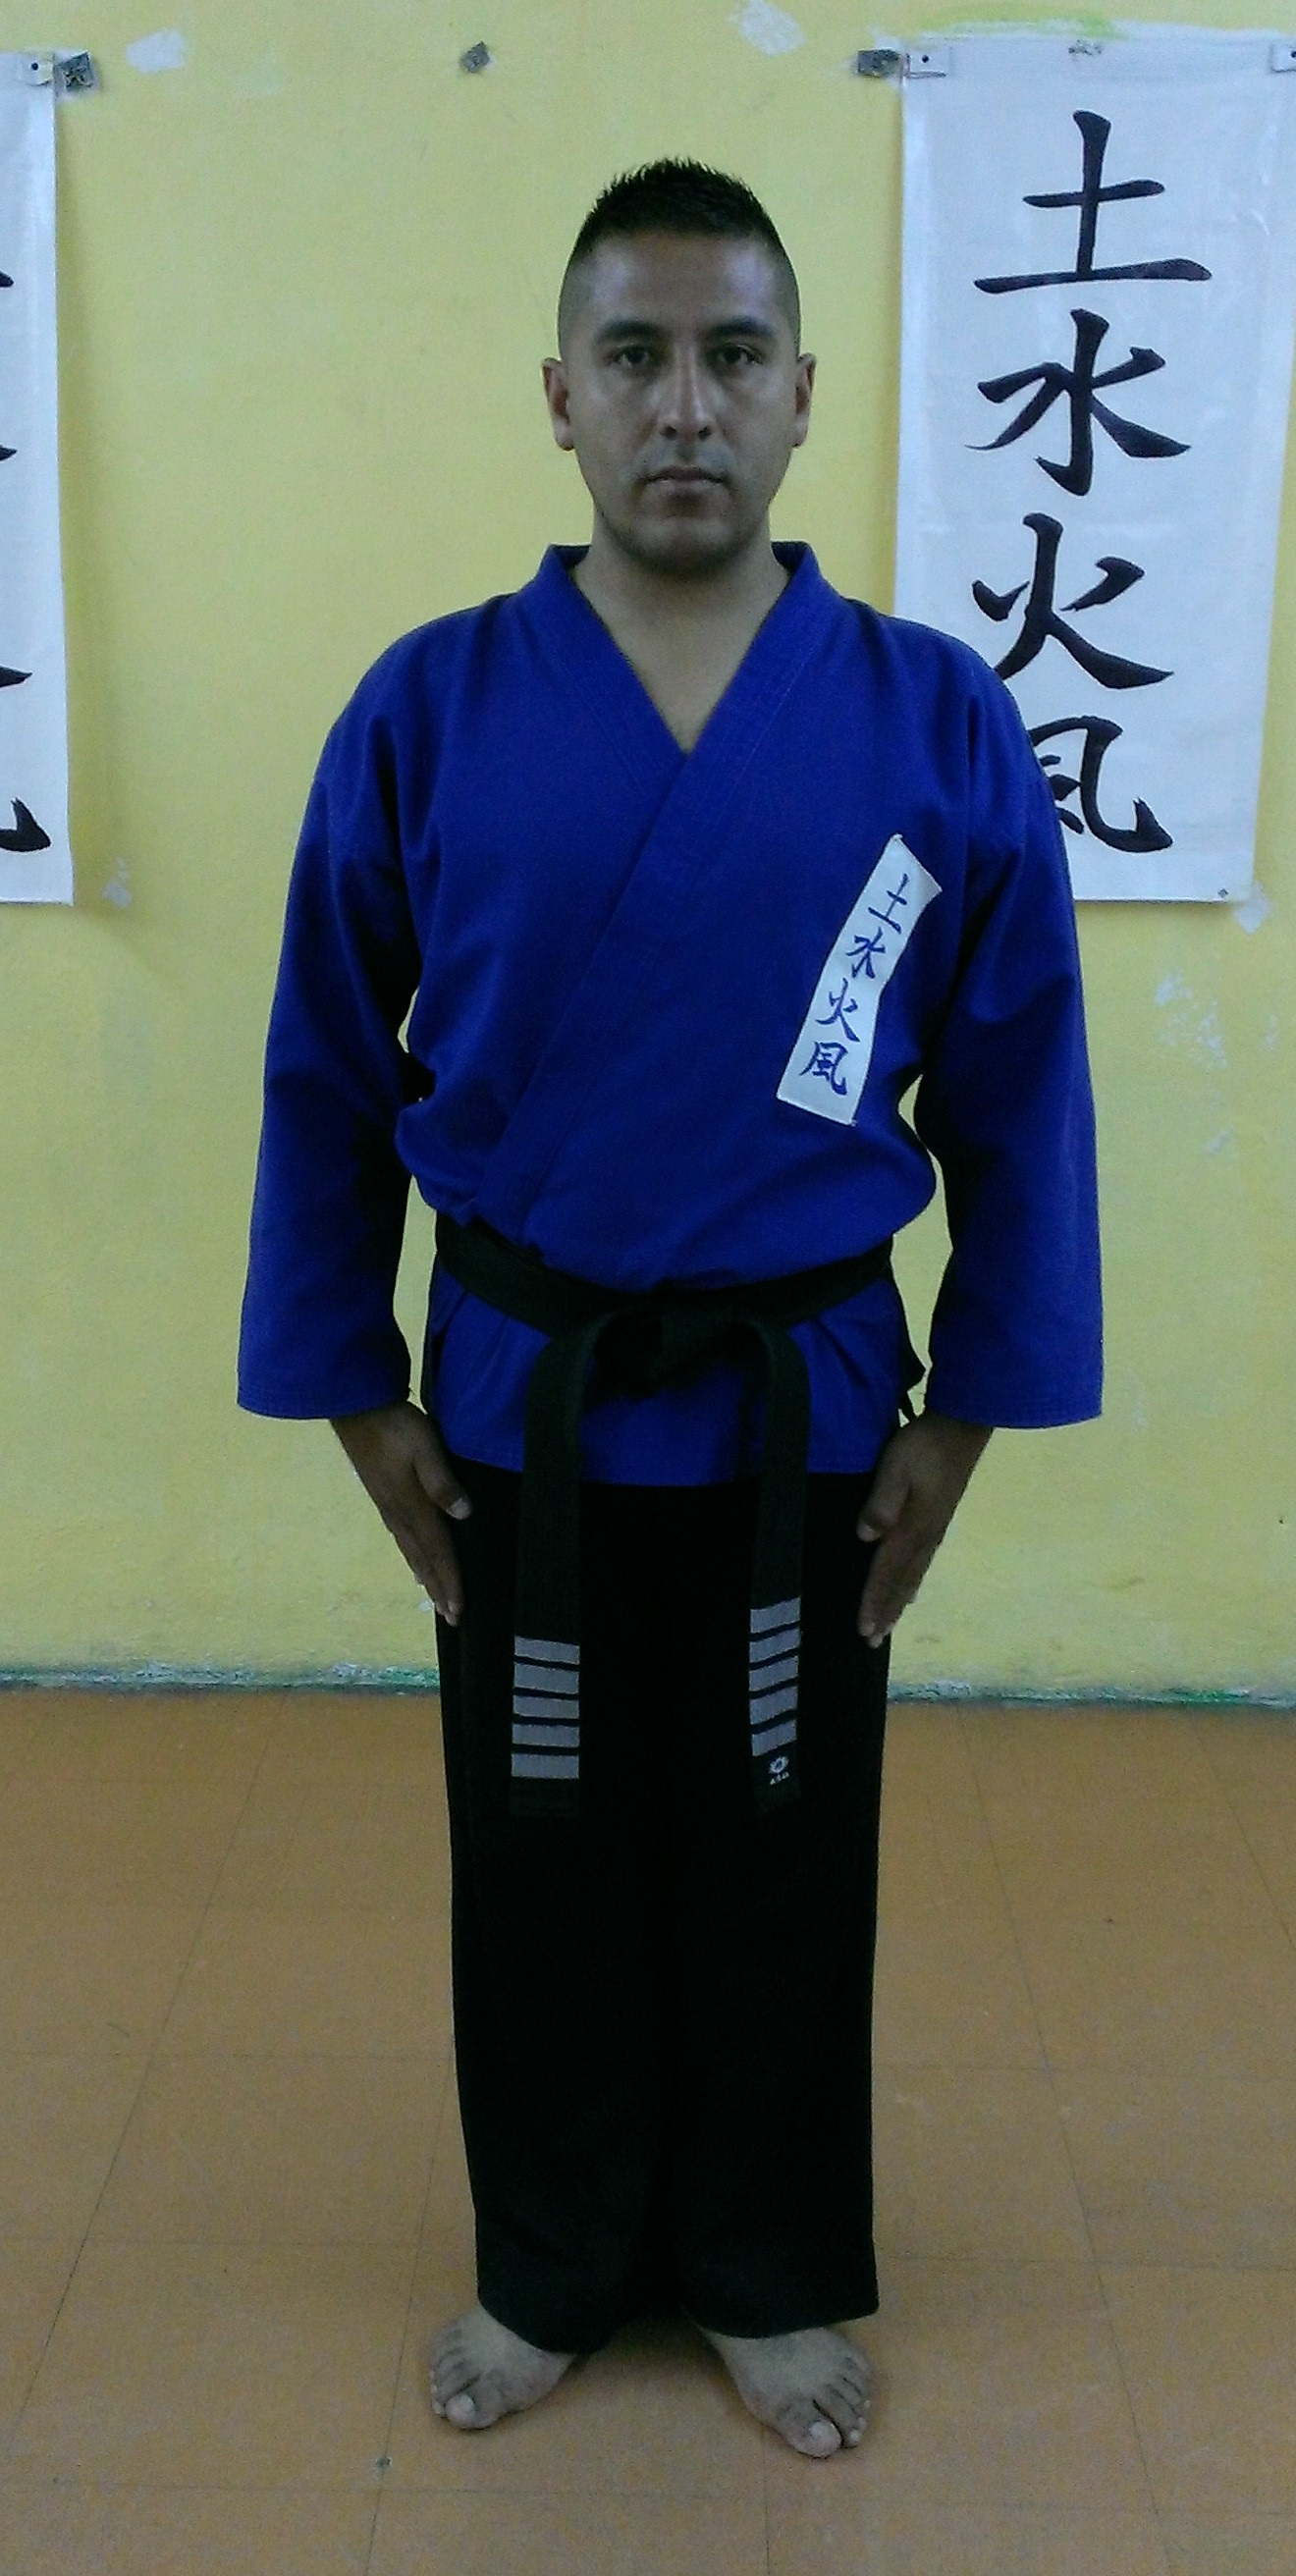
\includegraphics[width=4.5cm, height=8cm]{./Figuras/Tecnica/Musubidachi_Frontal}}
	\subfloat[Hachiji - dachi frontal]{
		\label{fig:Hachijidachi_Frontal}
		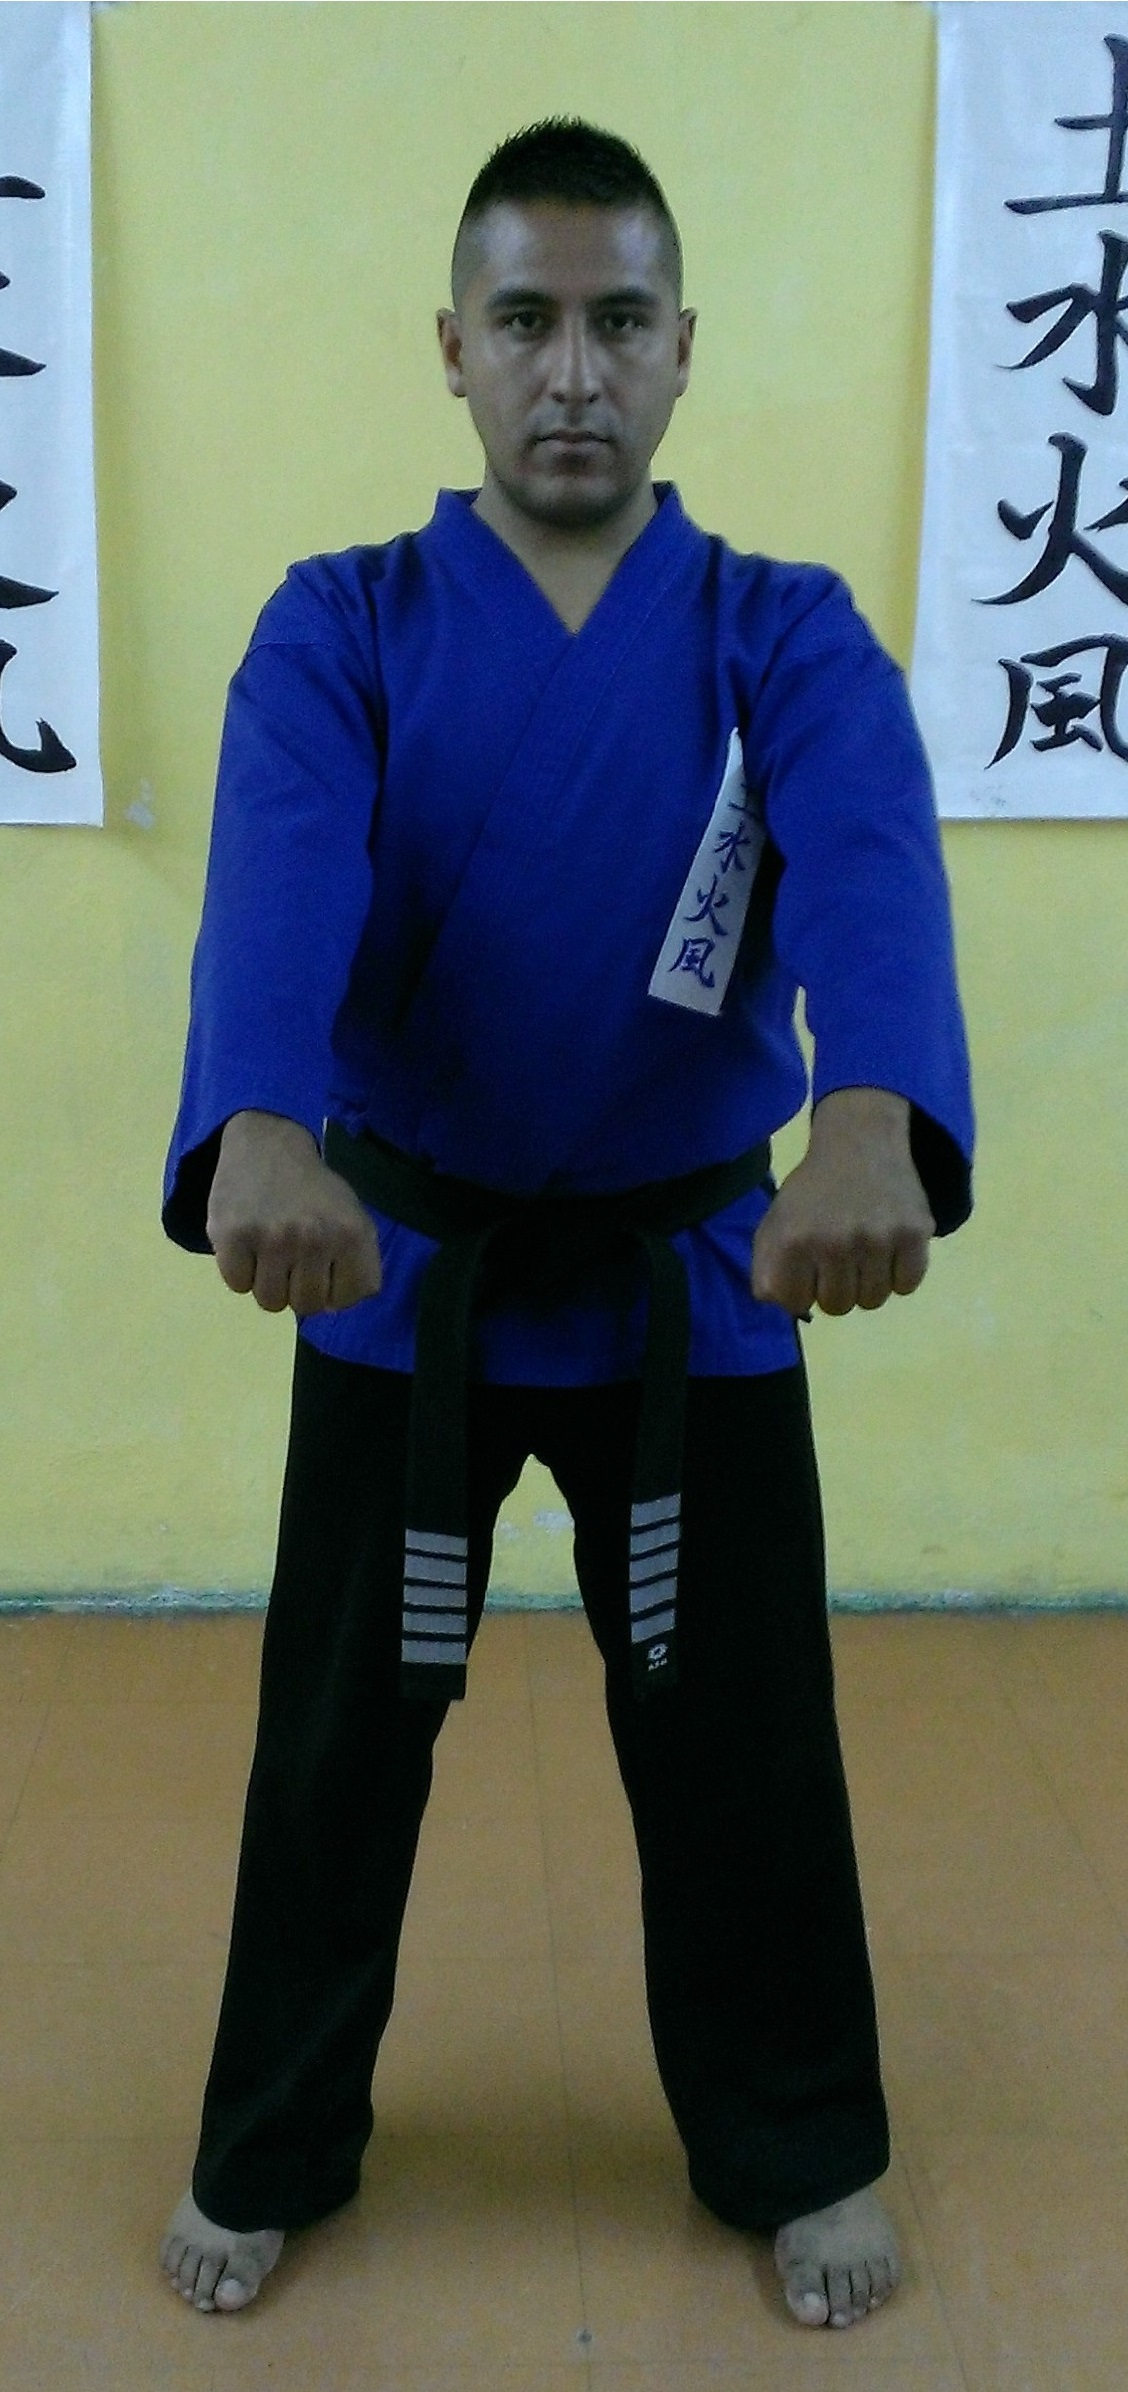
\includegraphics[width=4.5cm, height=8cm]{./Figuras/Tecnica/Hachijidachi_Frontal}}
	\caption{Posiciones Musubi - dachi y Hachiji - dachi }
	\label{fig:Posiciones1}
\end{figure}

\begin{figure}[H]
	\centering
	\subfloat[Posición Senkuntsu - dachi frontal]{
		\label{fig:Senkuntsudachi_Frontal}
		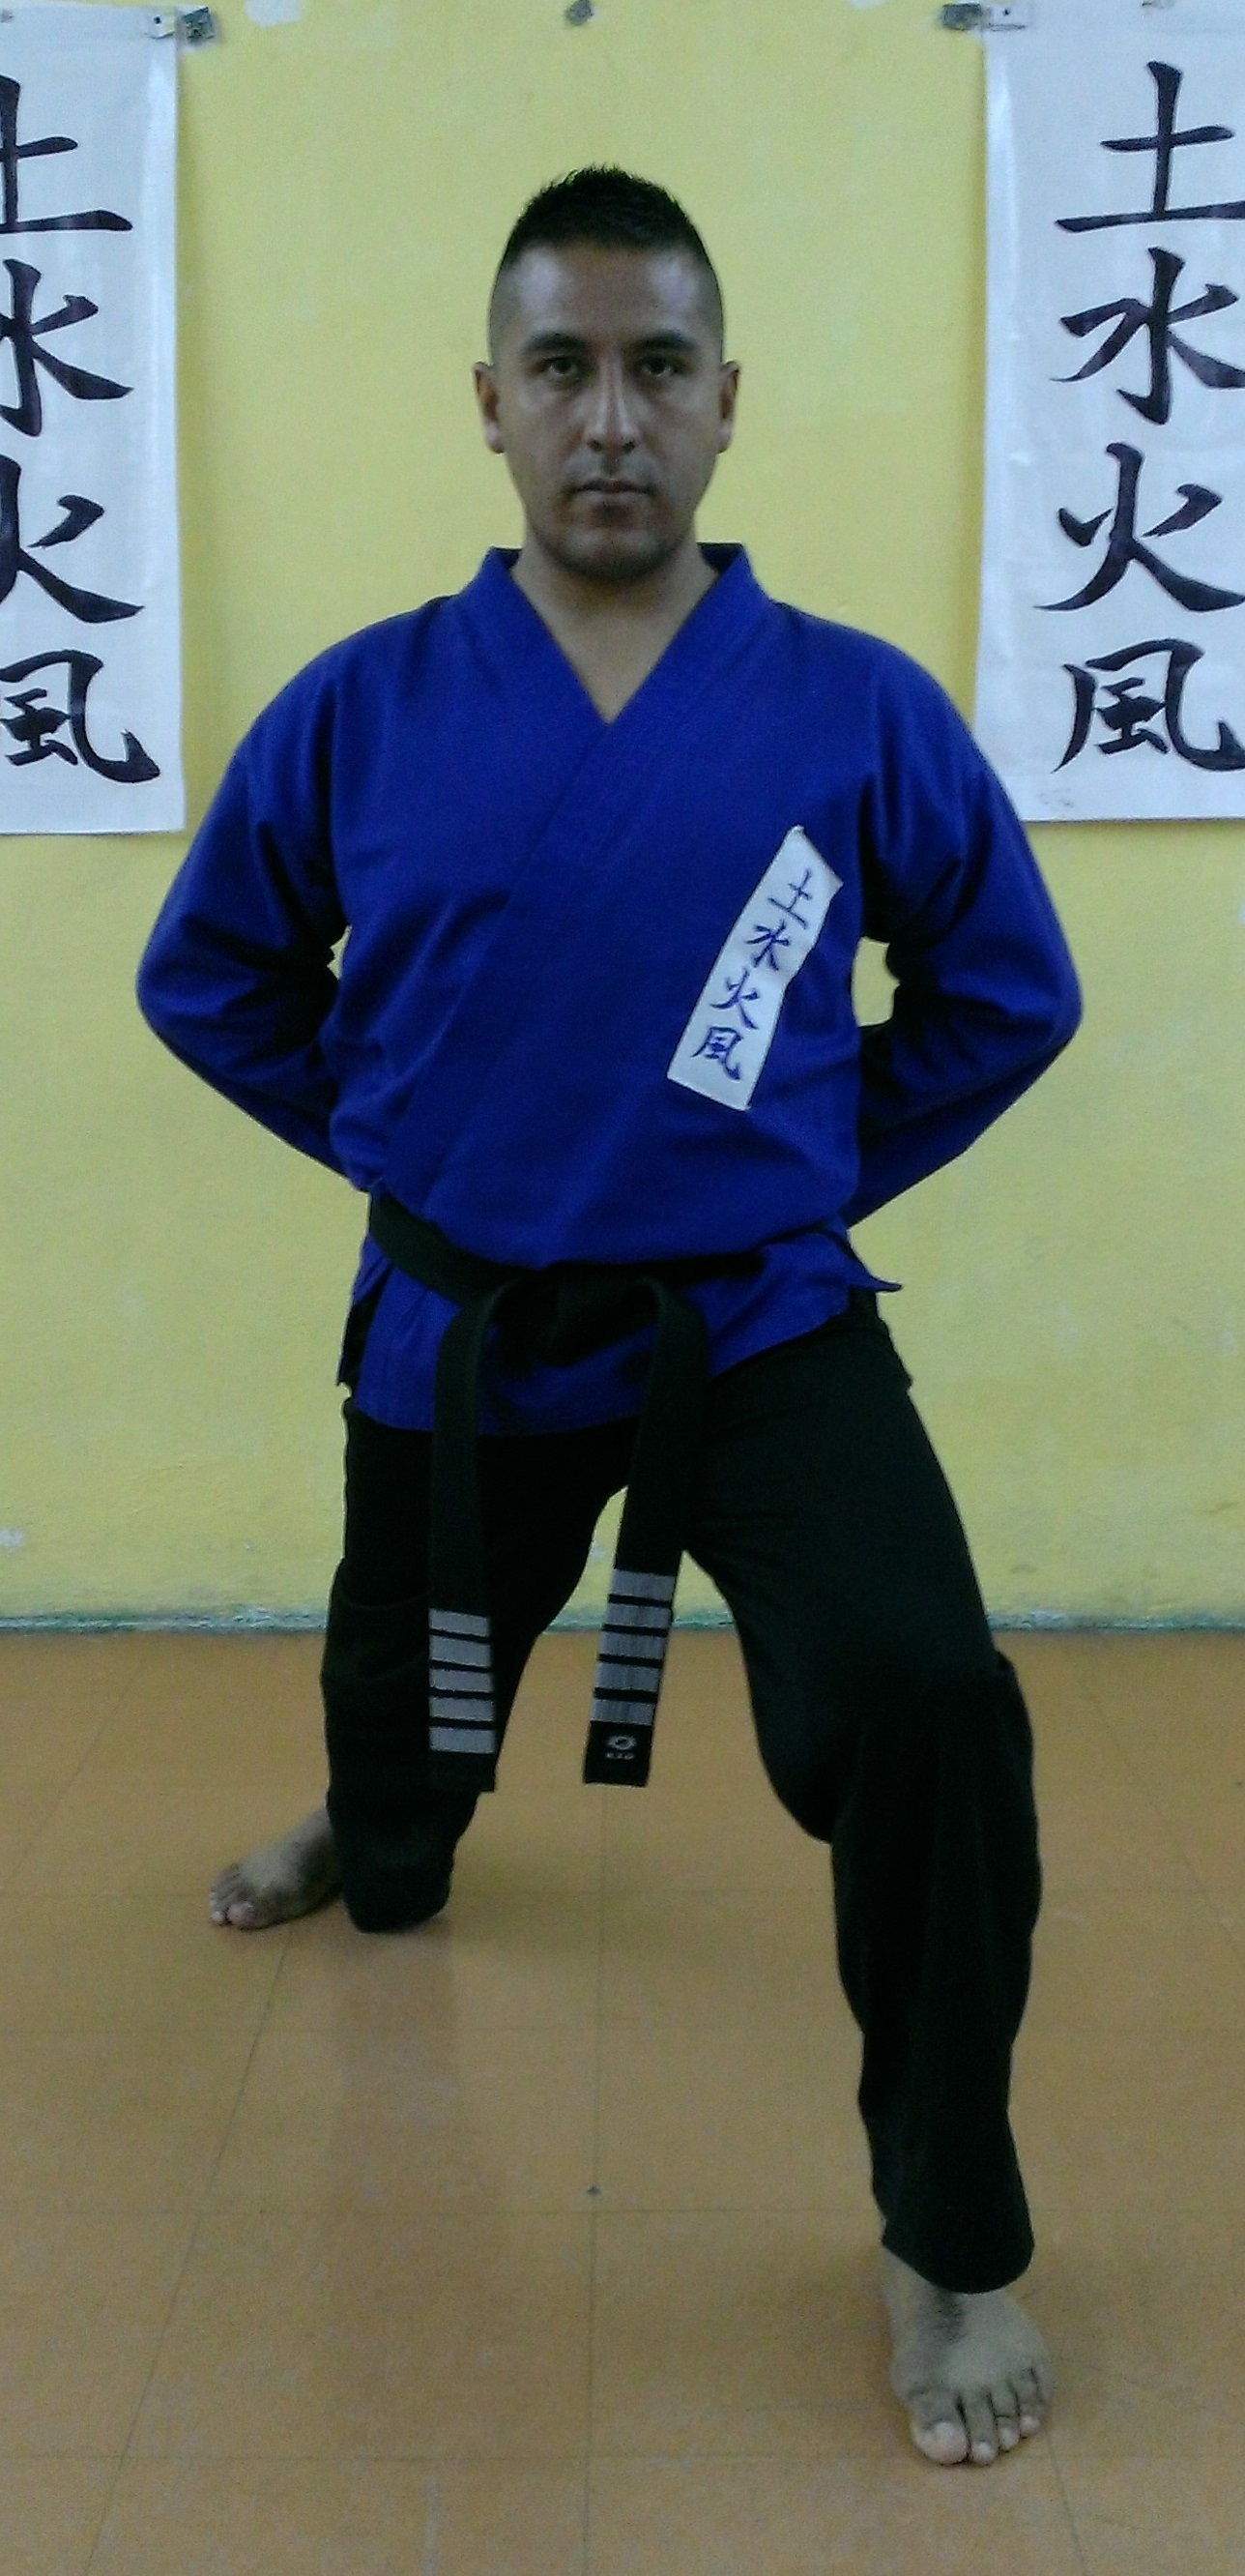
\includegraphics[width=4.5cm, height=8cm]{./Figuras/Tecnica/Senkuntsudachi_Frontal}}
	\subfloat[Posición Senkuntsu - dachi lateral]{
		\label{fig:Senkuntsudachi_Lateral}
		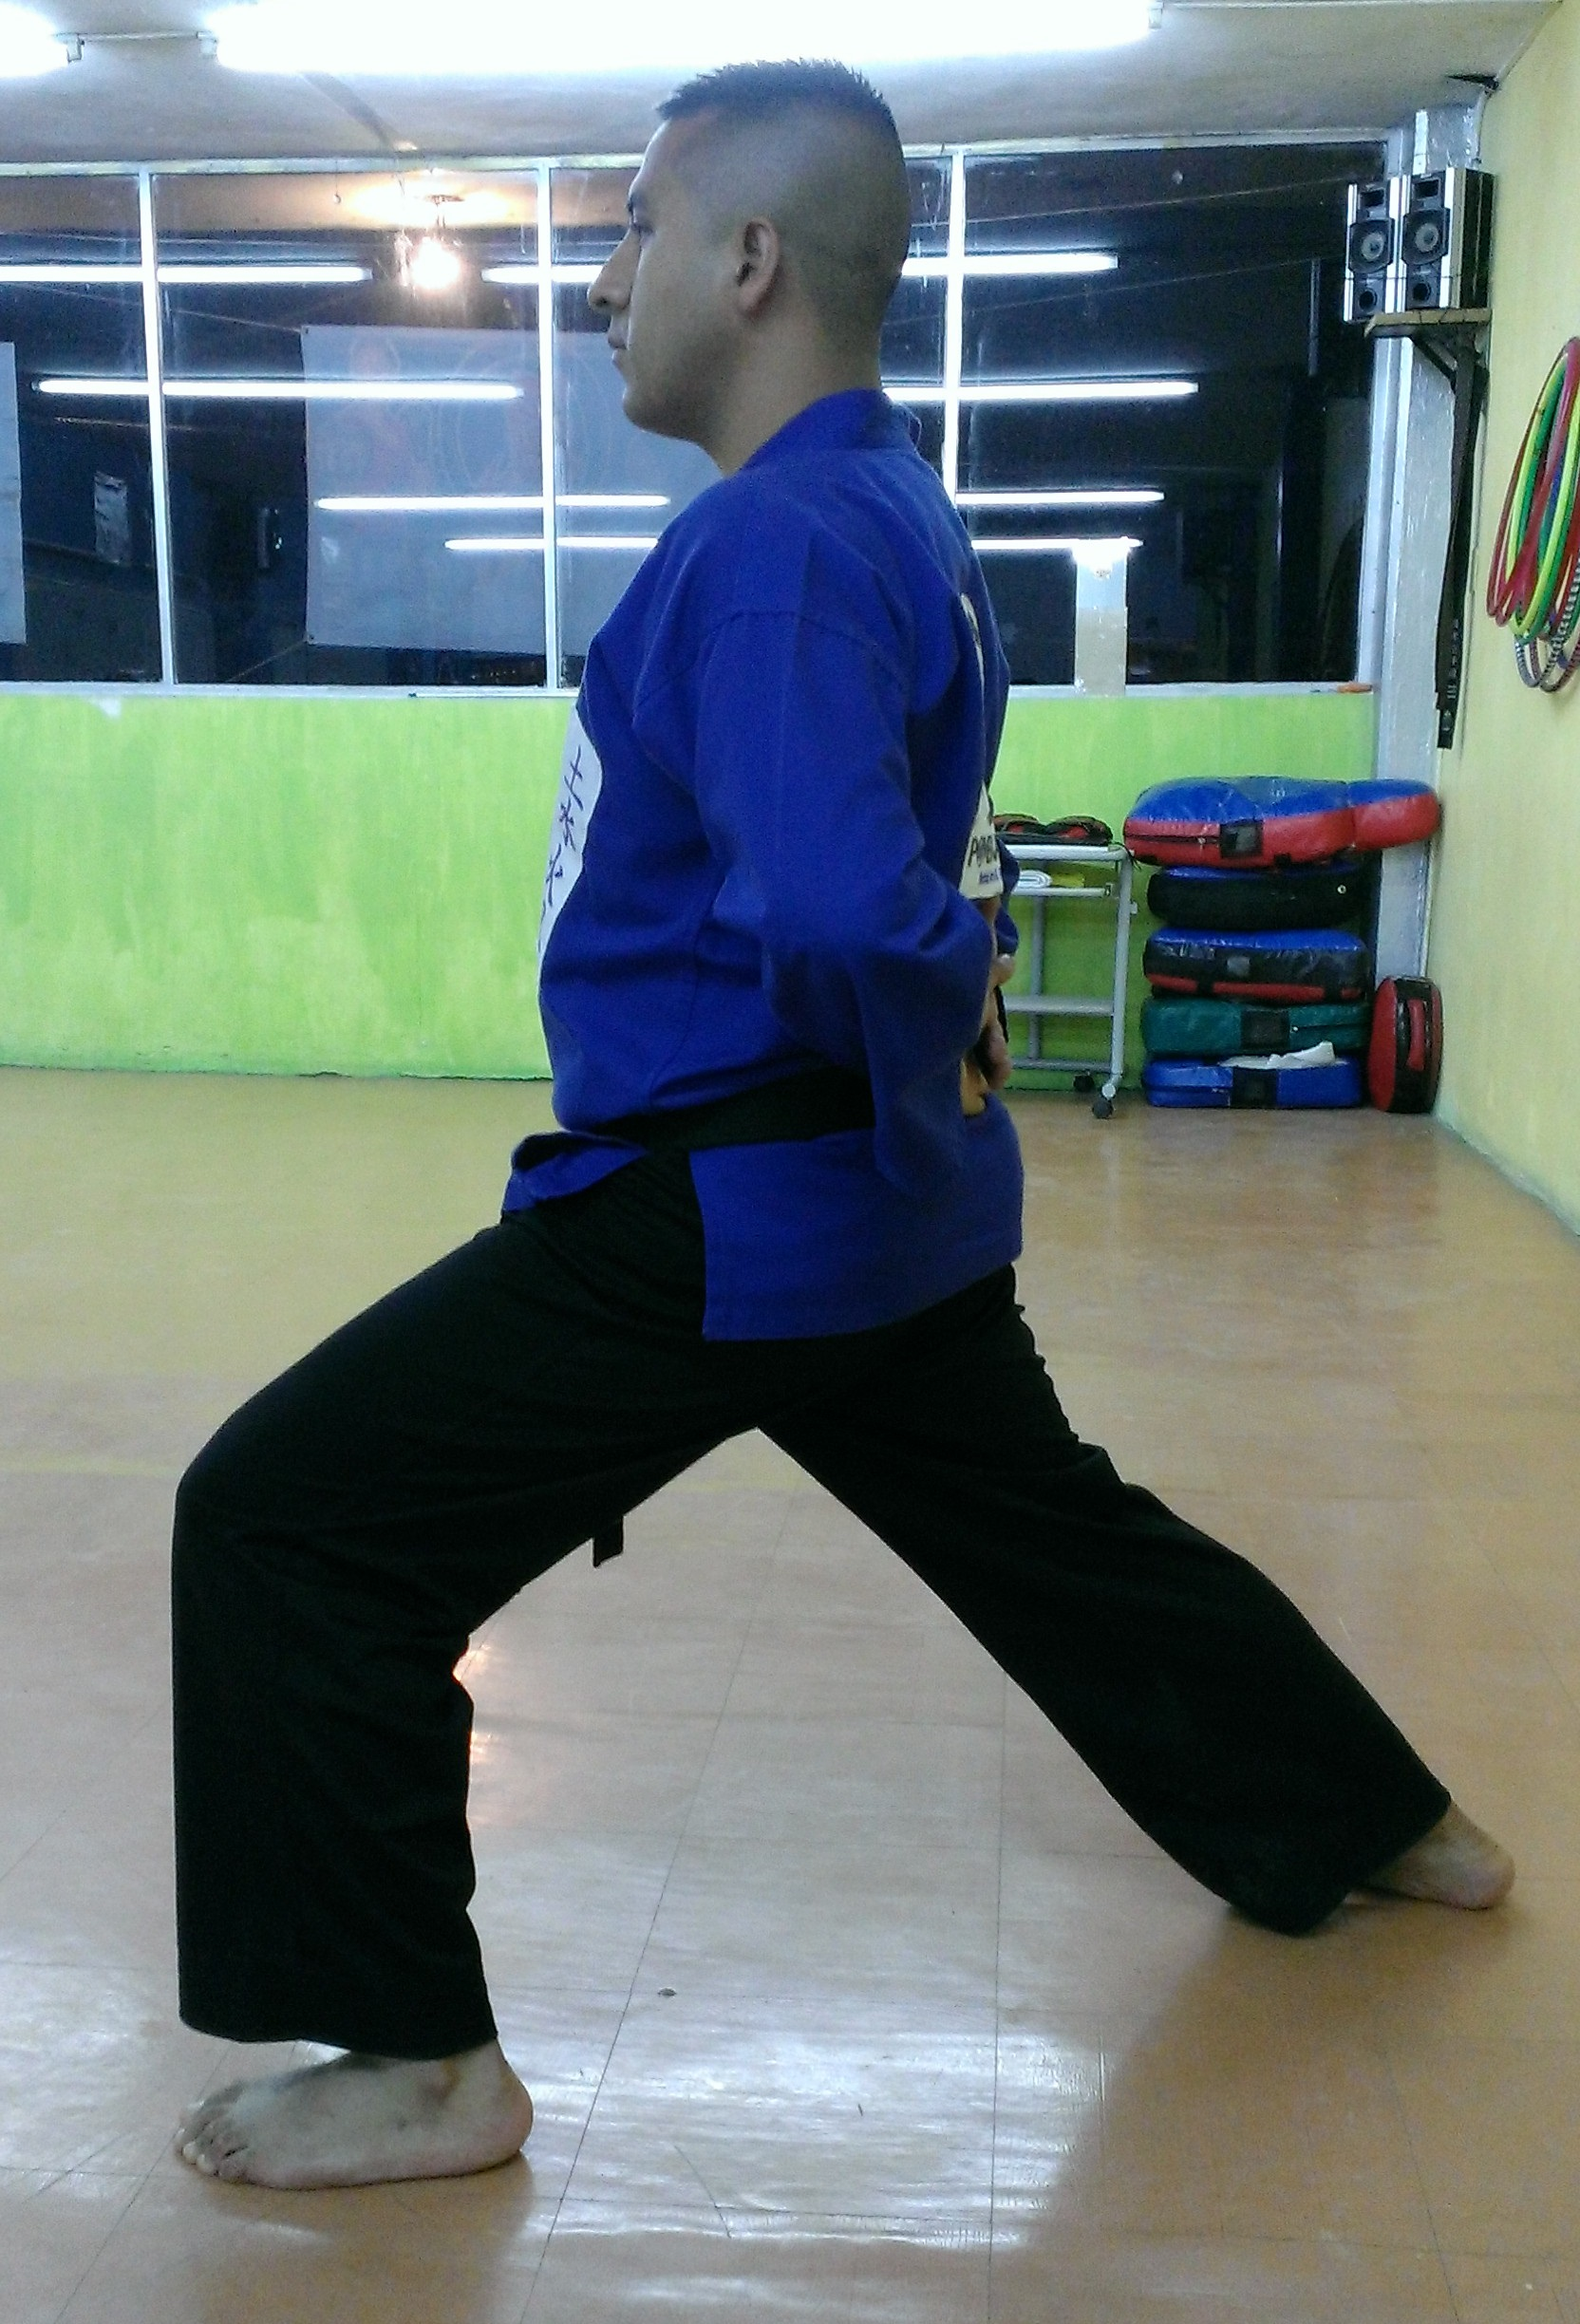
\includegraphics[width=5.5cm, height=8cm]{./Figuras/Tecnica/Senkuntsudachi_Lateral}}
	\caption{Posición Senkuntsu - dachi}
	\label{fig:Posiciones2}
\end{figure}

\begin{figure}[H]
	\centering
	\subfloat[Defensa Gedan Barai Uke frontal]{
		\label{fig:GedanBaraiUke_Frontal}
		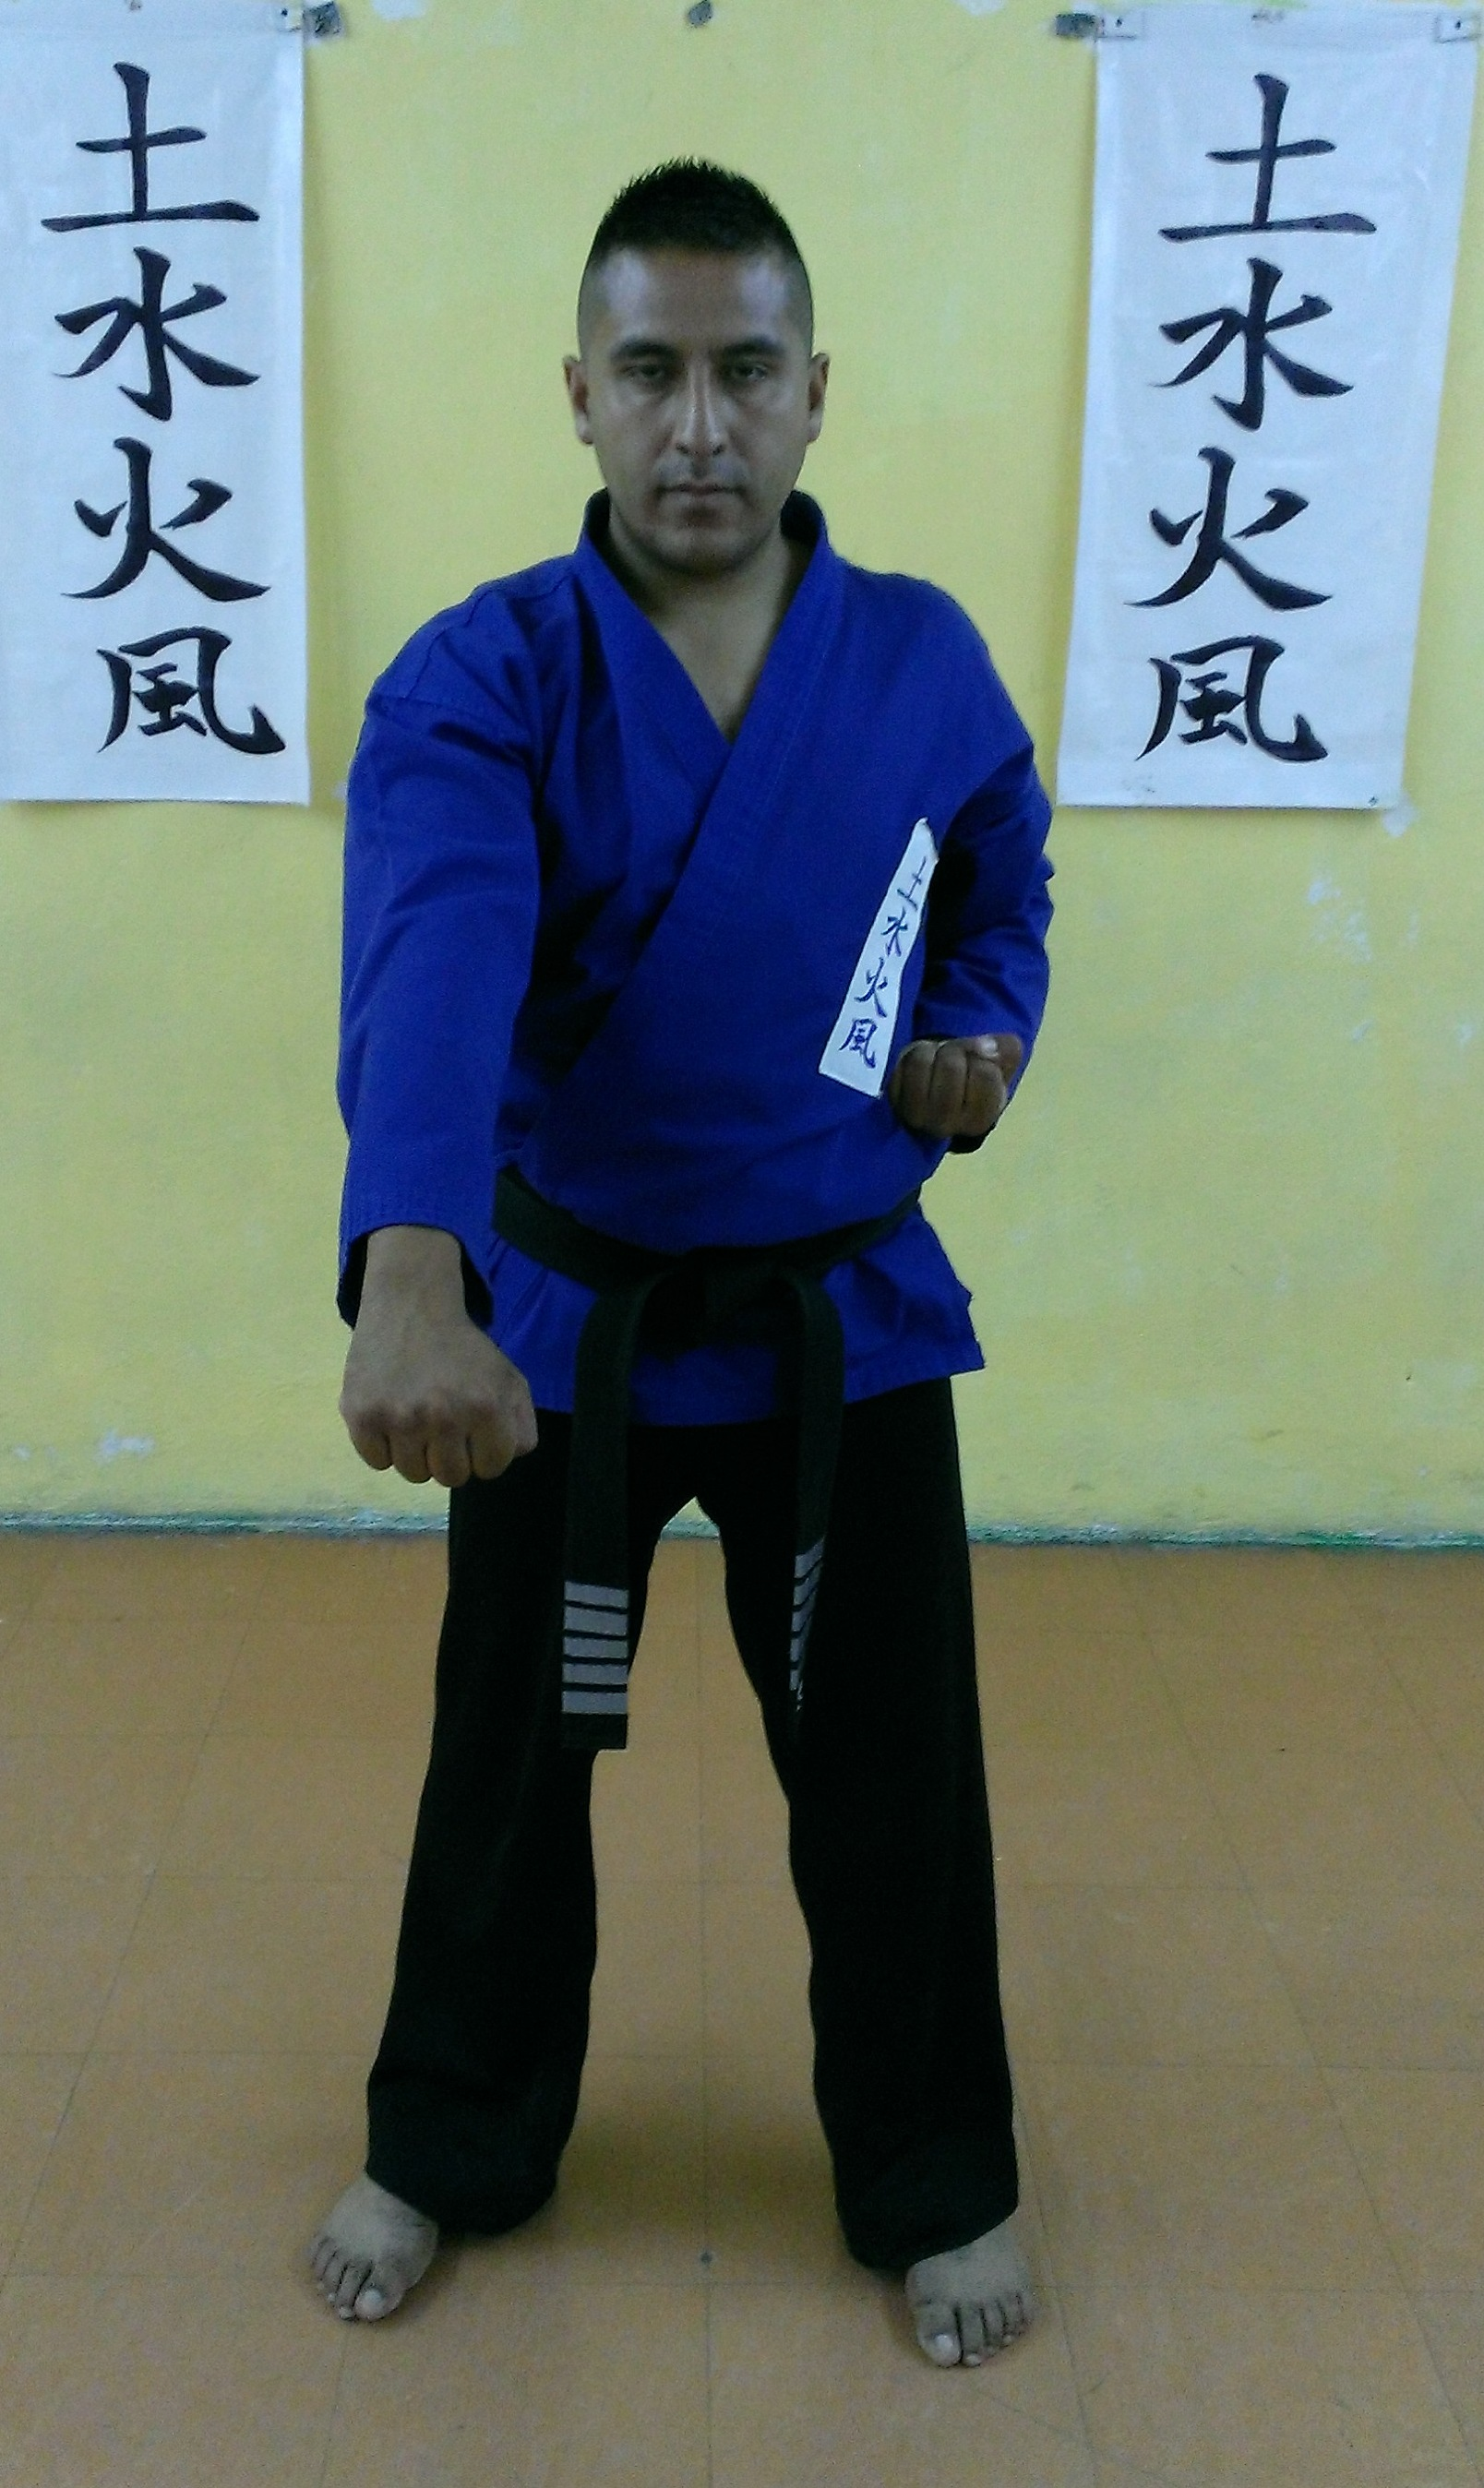
\includegraphics[width=5cm, height=8cm]{./Figuras/Tecnica/GedanBaraiUke_Frontal}}
	\subfloat[Defensa Gedan Barai Uke lateral]{
		\label{fig:GedanBaraiUke_Lateral}
		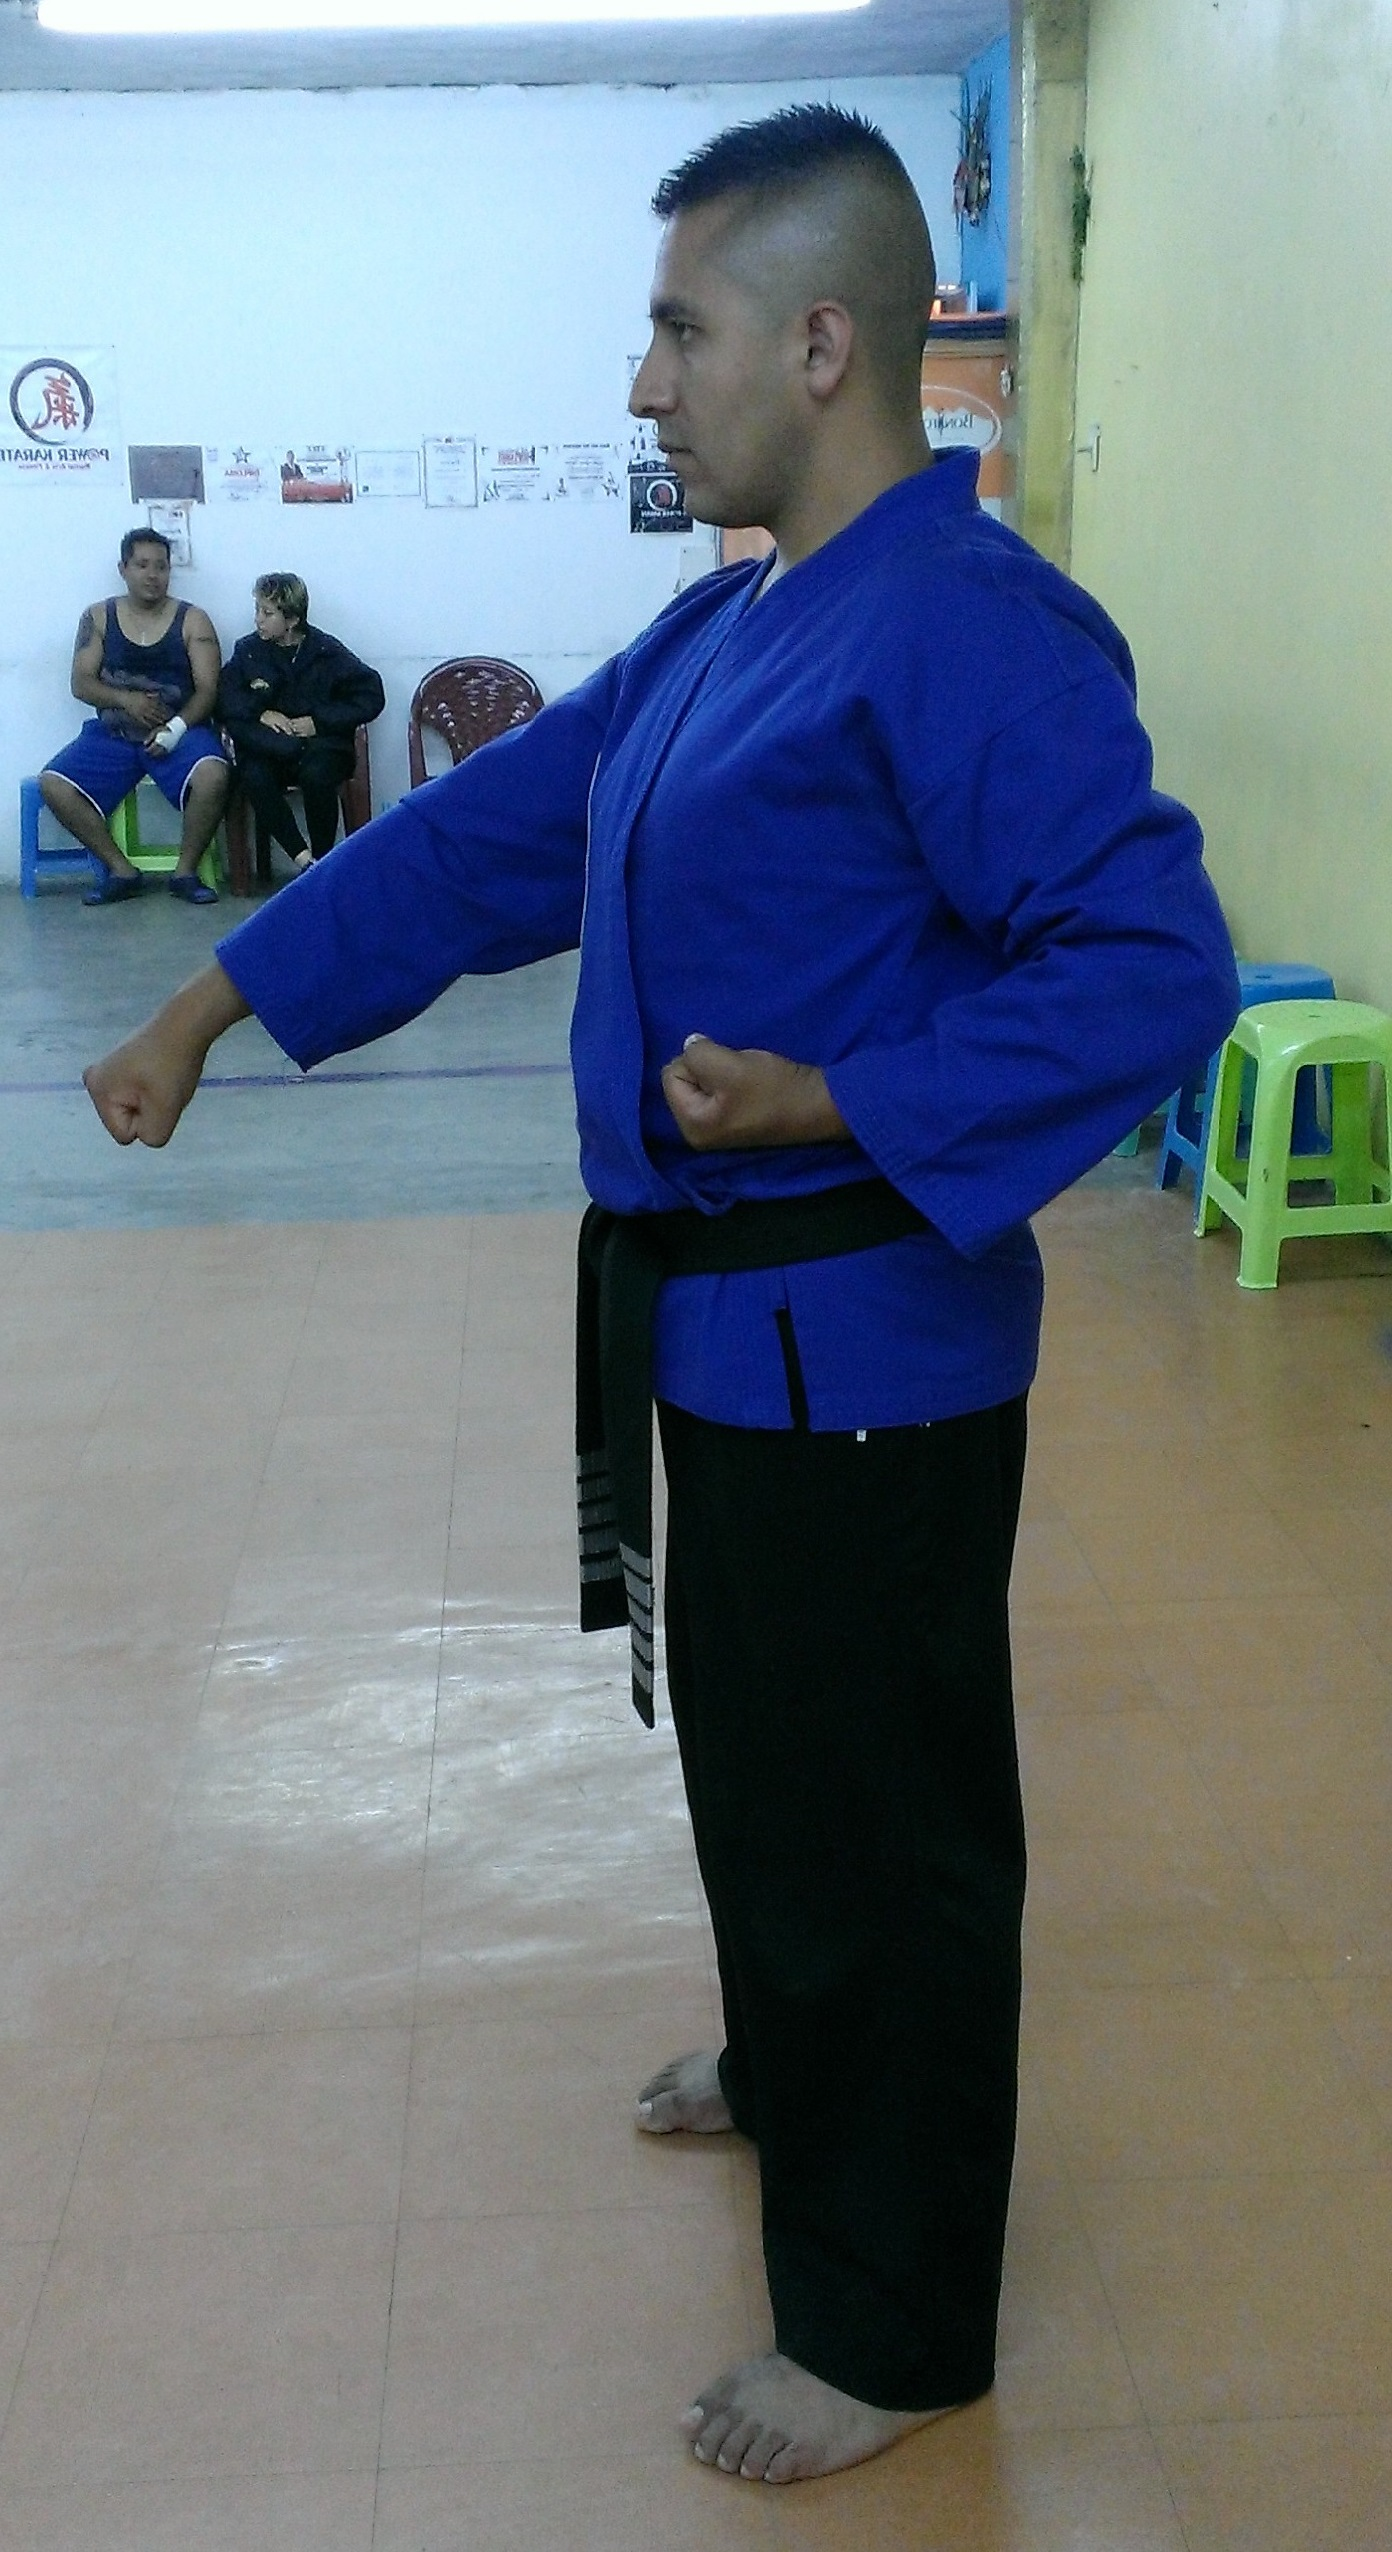
\includegraphics[width=5cm, height=8cm]{./Figuras/Tecnica/GedanBaraiUke_Lateral}}
	\caption{Defensa Gedan Barai Uke}
	\label{fig:Defensas1}
\end{figure}

\begin{figure}[H]
	\centering
	\subfloat[Defensa Shudan Soto Uke frontal]{
		\label{fig:ShudanSotoUke_Frontal}
		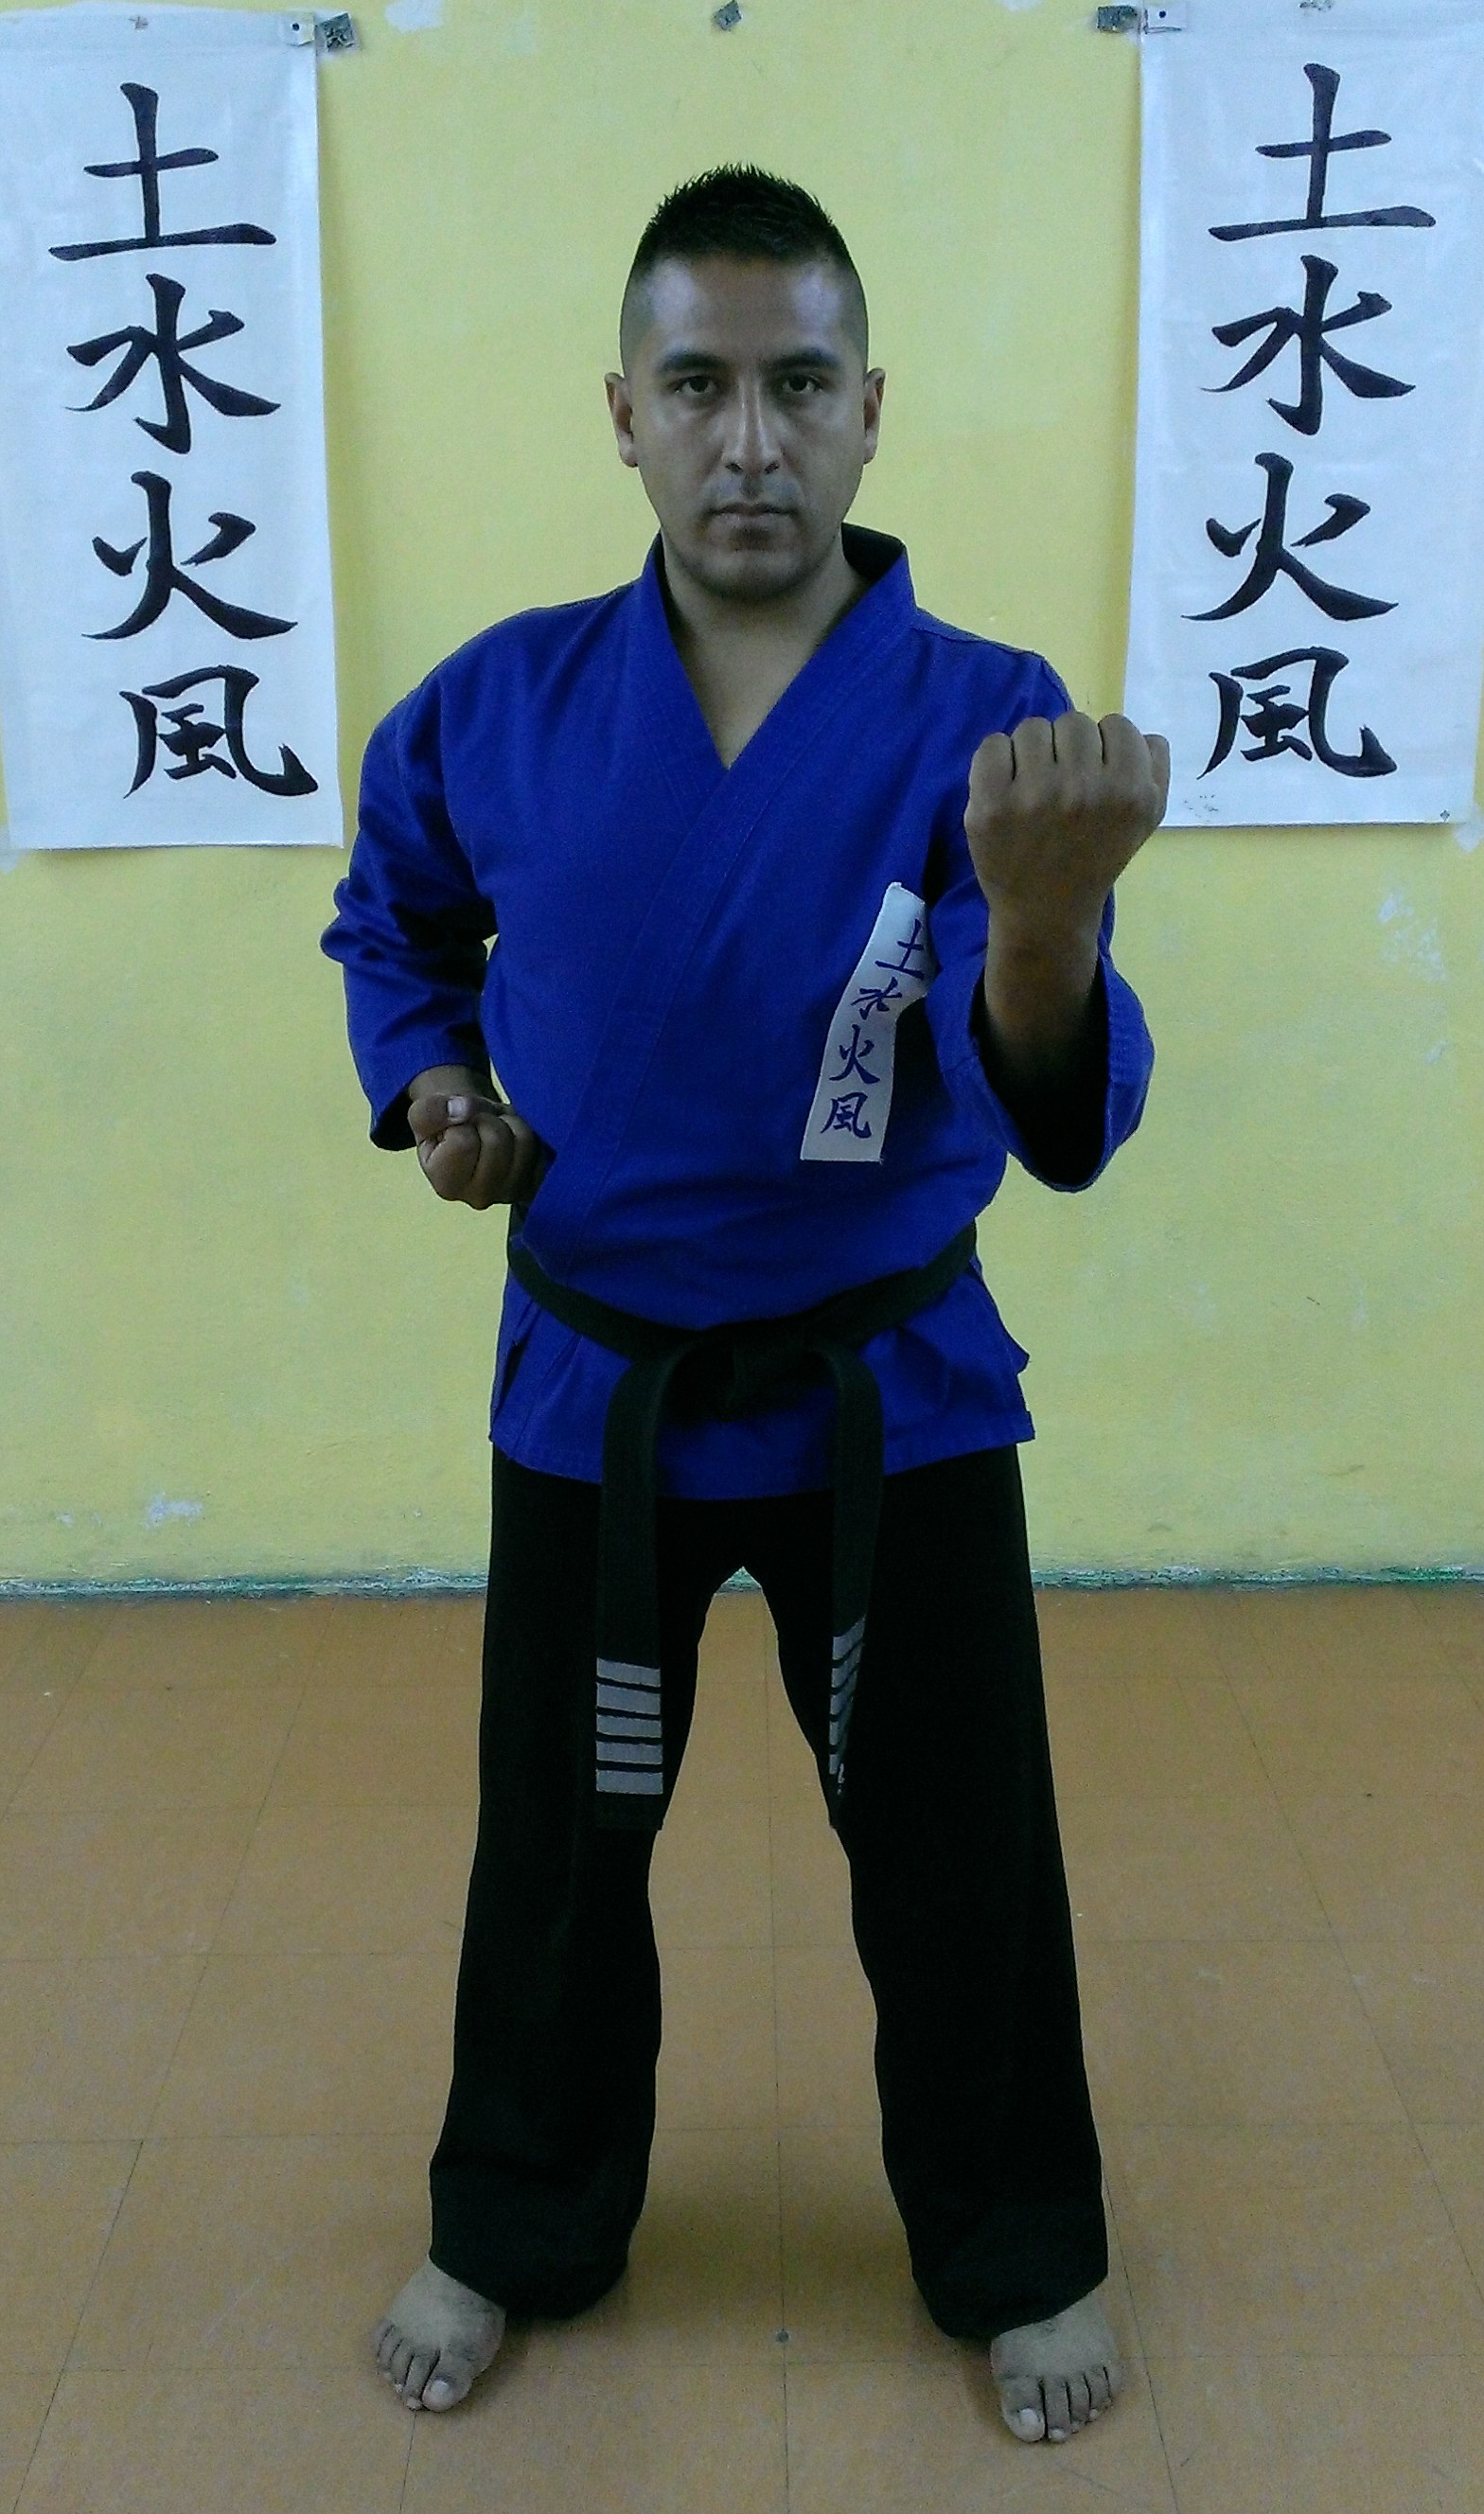
\includegraphics[width=5cm, height=8cm]{./Figuras/Tecnica/ShudanSotoUke_Frontal}}
	\subfloat[Defensa Shudan Soto Uke lateral]{
		\label{fig:ShudanSotoUke_Lateral}
		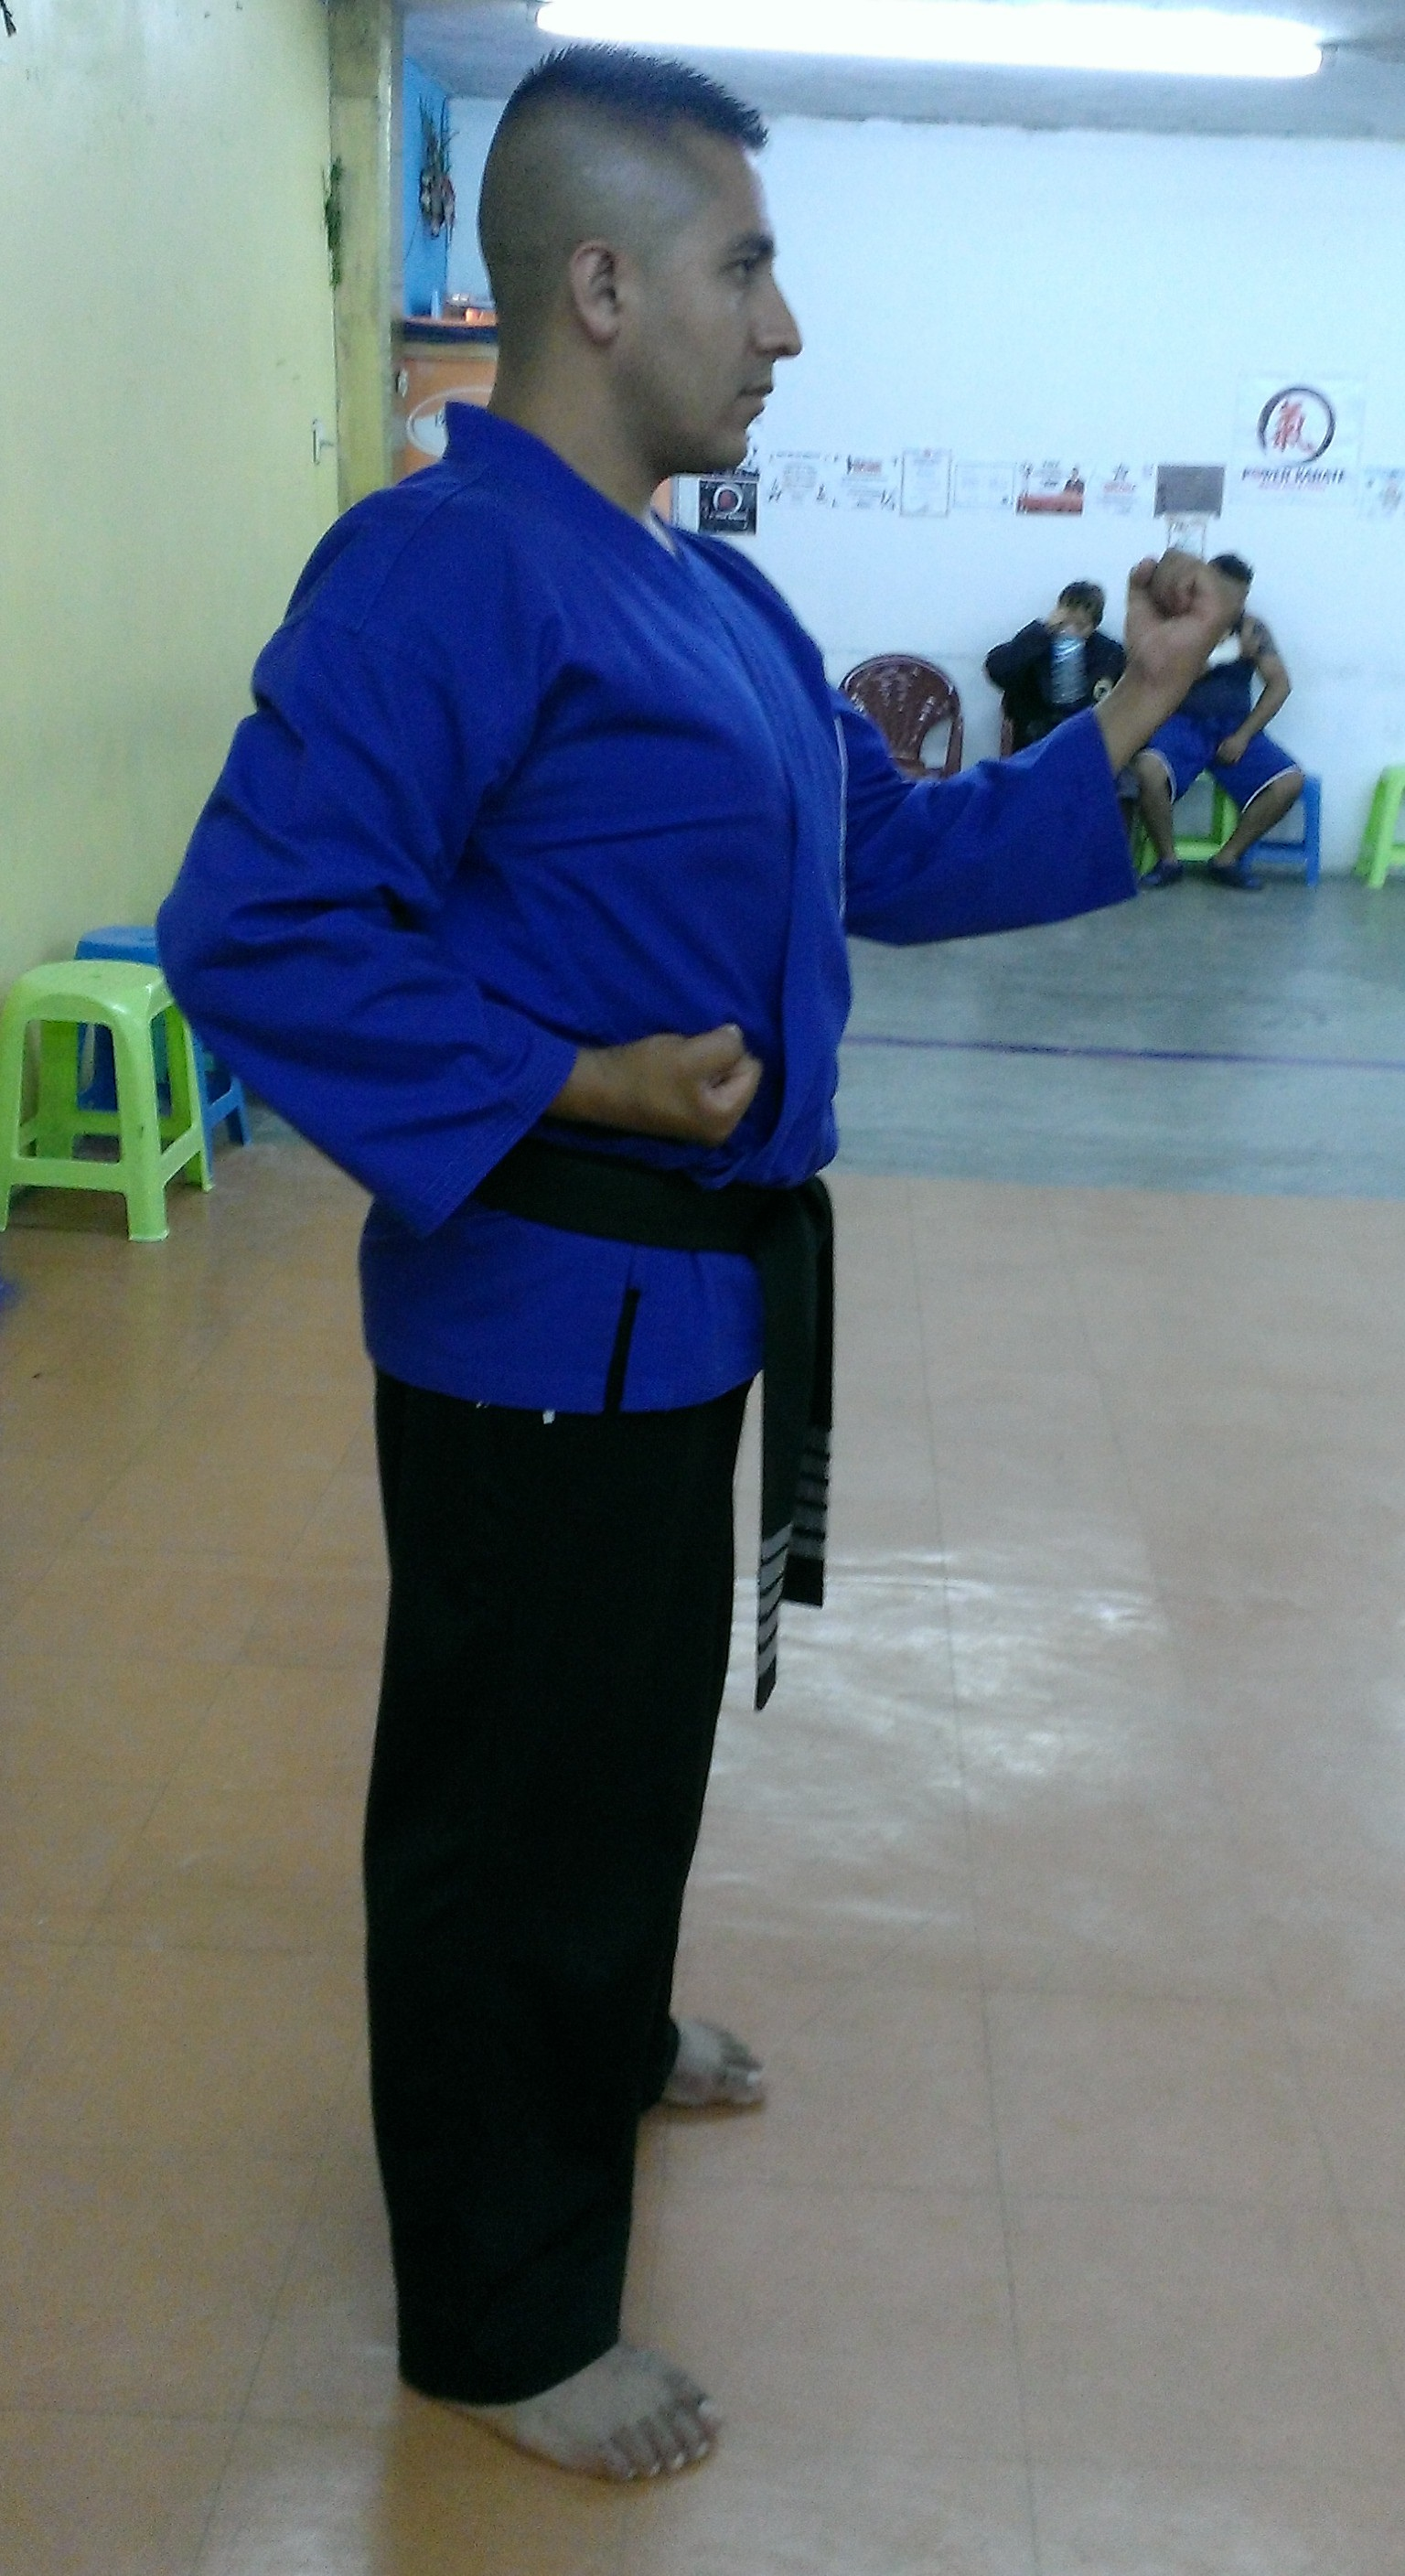
\includegraphics[width=5cm, height=8cm]{./Figuras/Tecnica/ShudanSotoUke_Lateral}}
	\caption{Defensa Shudan Soto Uke}
	\label{fig:Defensas2}
\end{figure}

\begin{figure}[H]
	\centering
	\subfloat[Defensa Yodan Age Uke frontal]{
		\label{fig:YodanAgeUke_Frontal}
		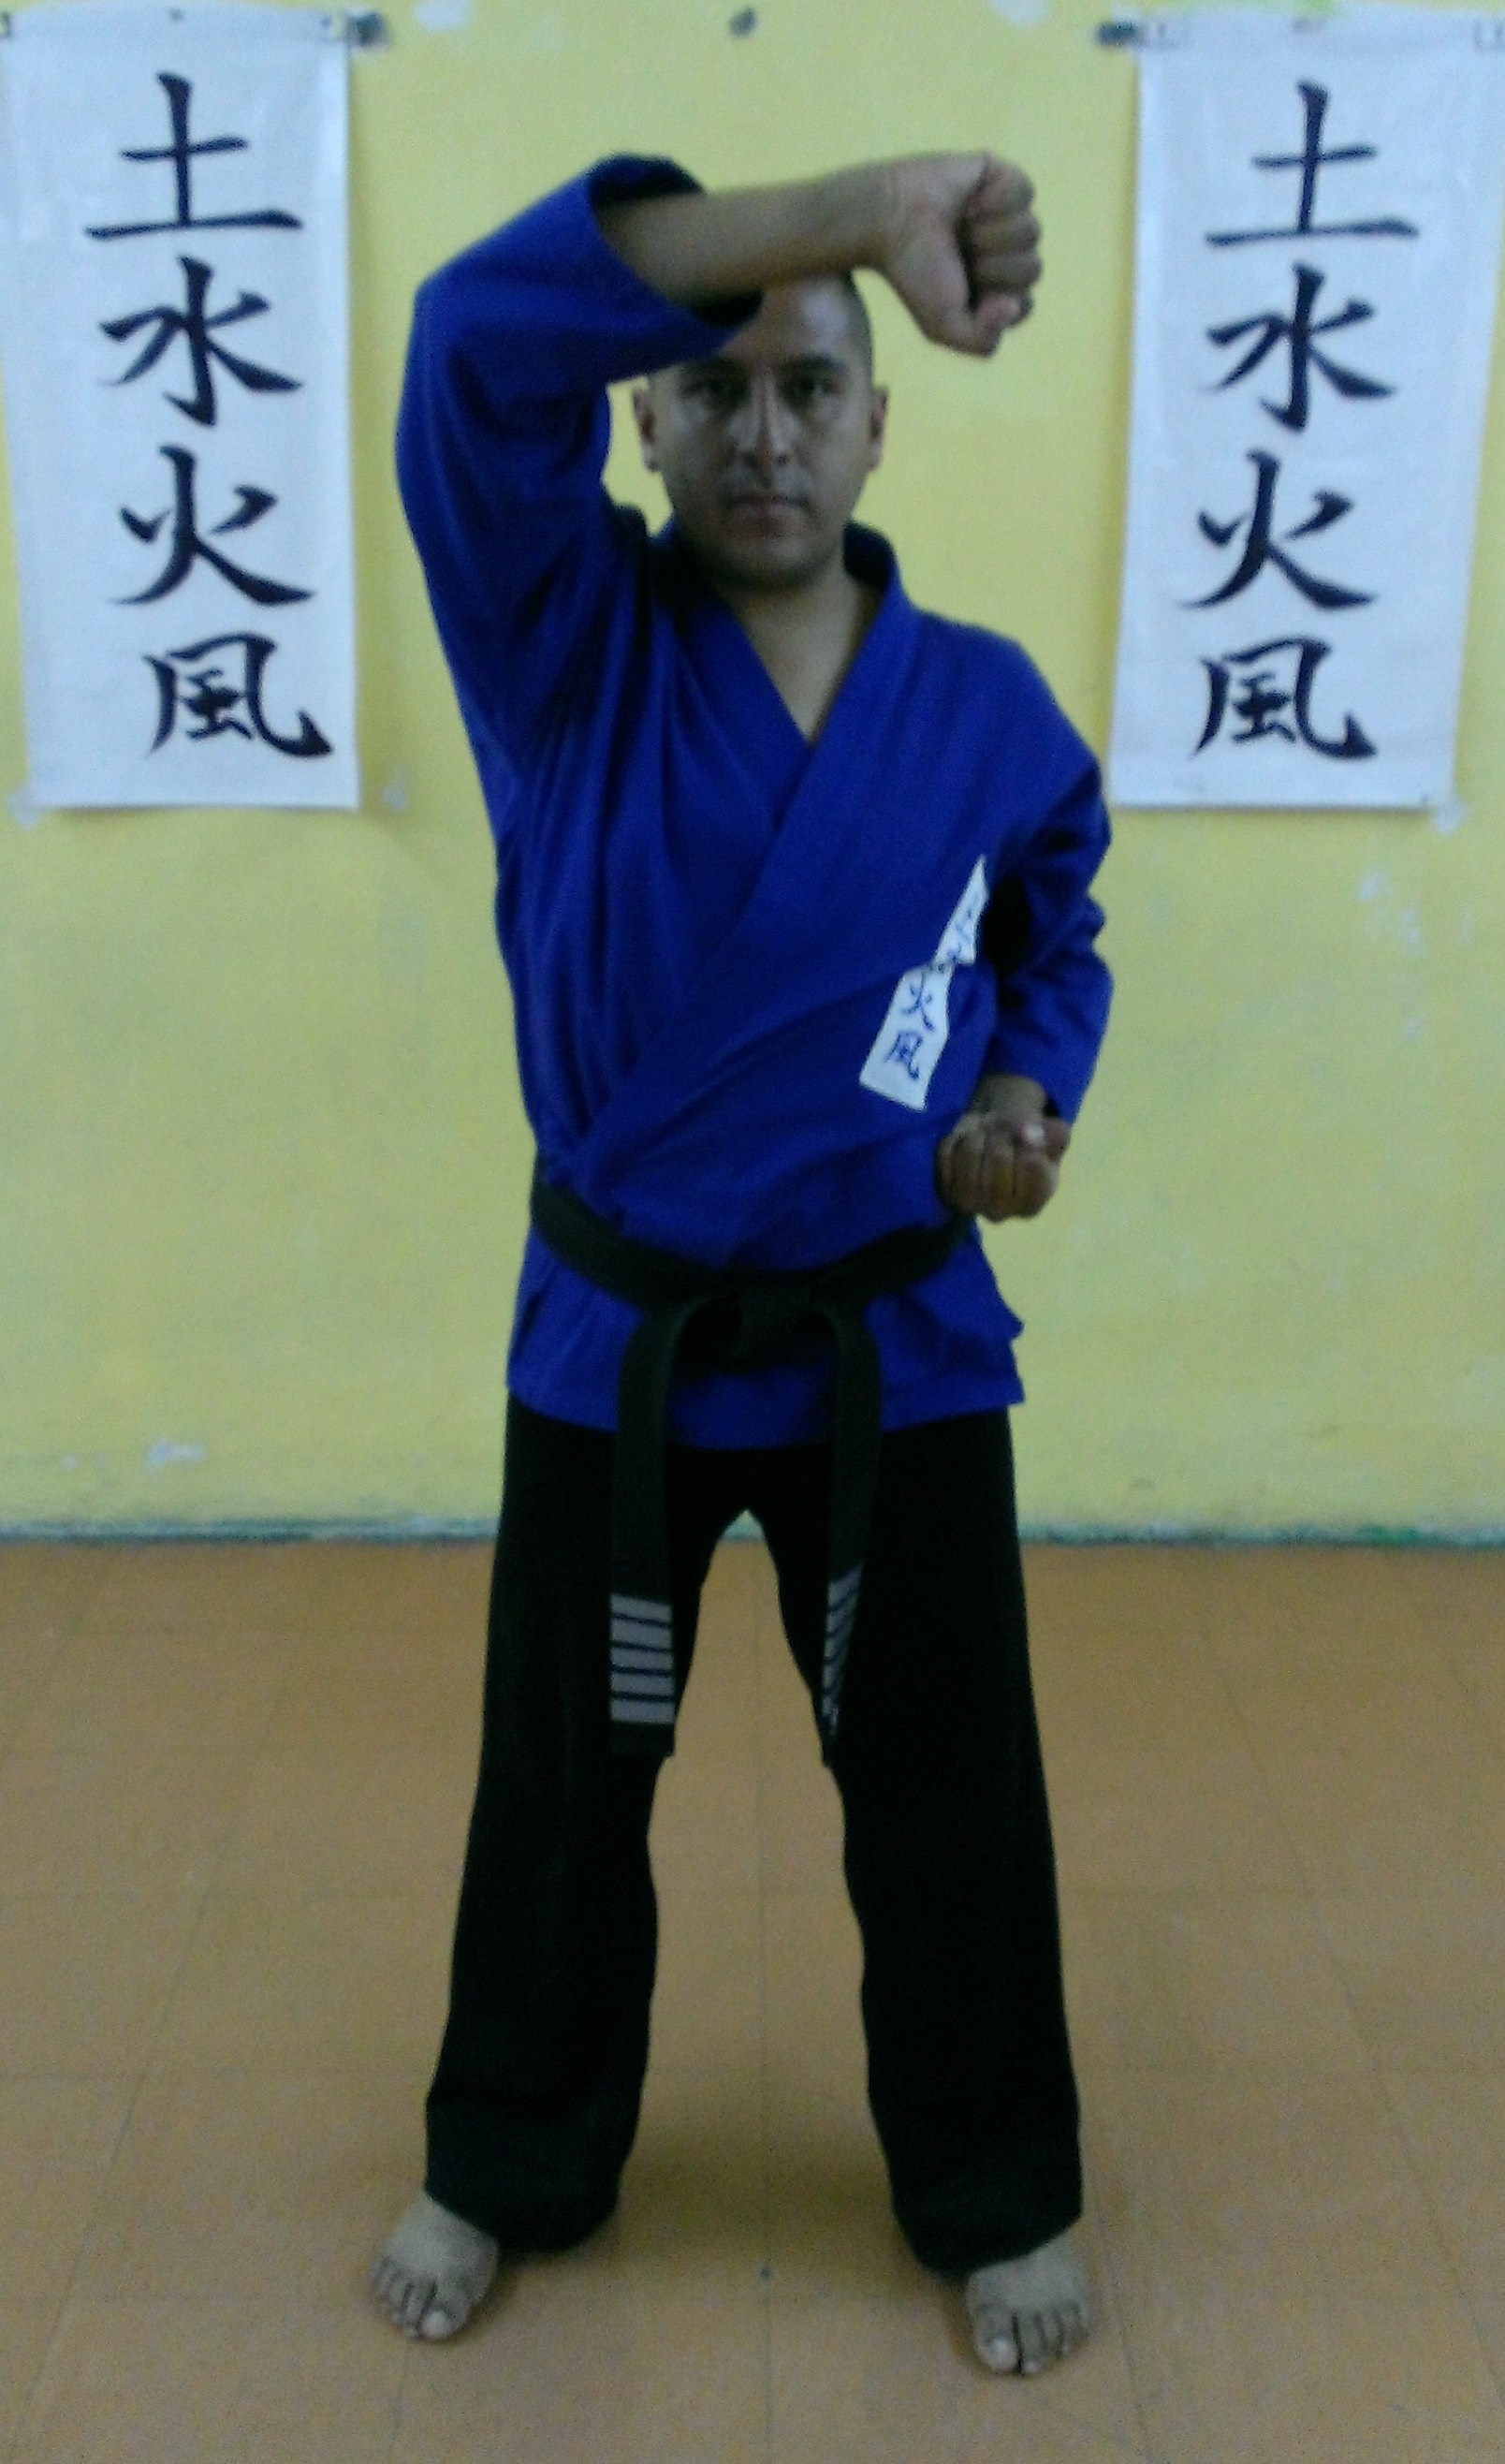
\includegraphics[width=5cm, height=8cm]{./Figuras/Tecnica/YodanAgeUke_Frontal}}
	\subfloat[Defensa Yodan Age Uke lateral]{
		\label{fig:YodanAgeUke_Lateral}
		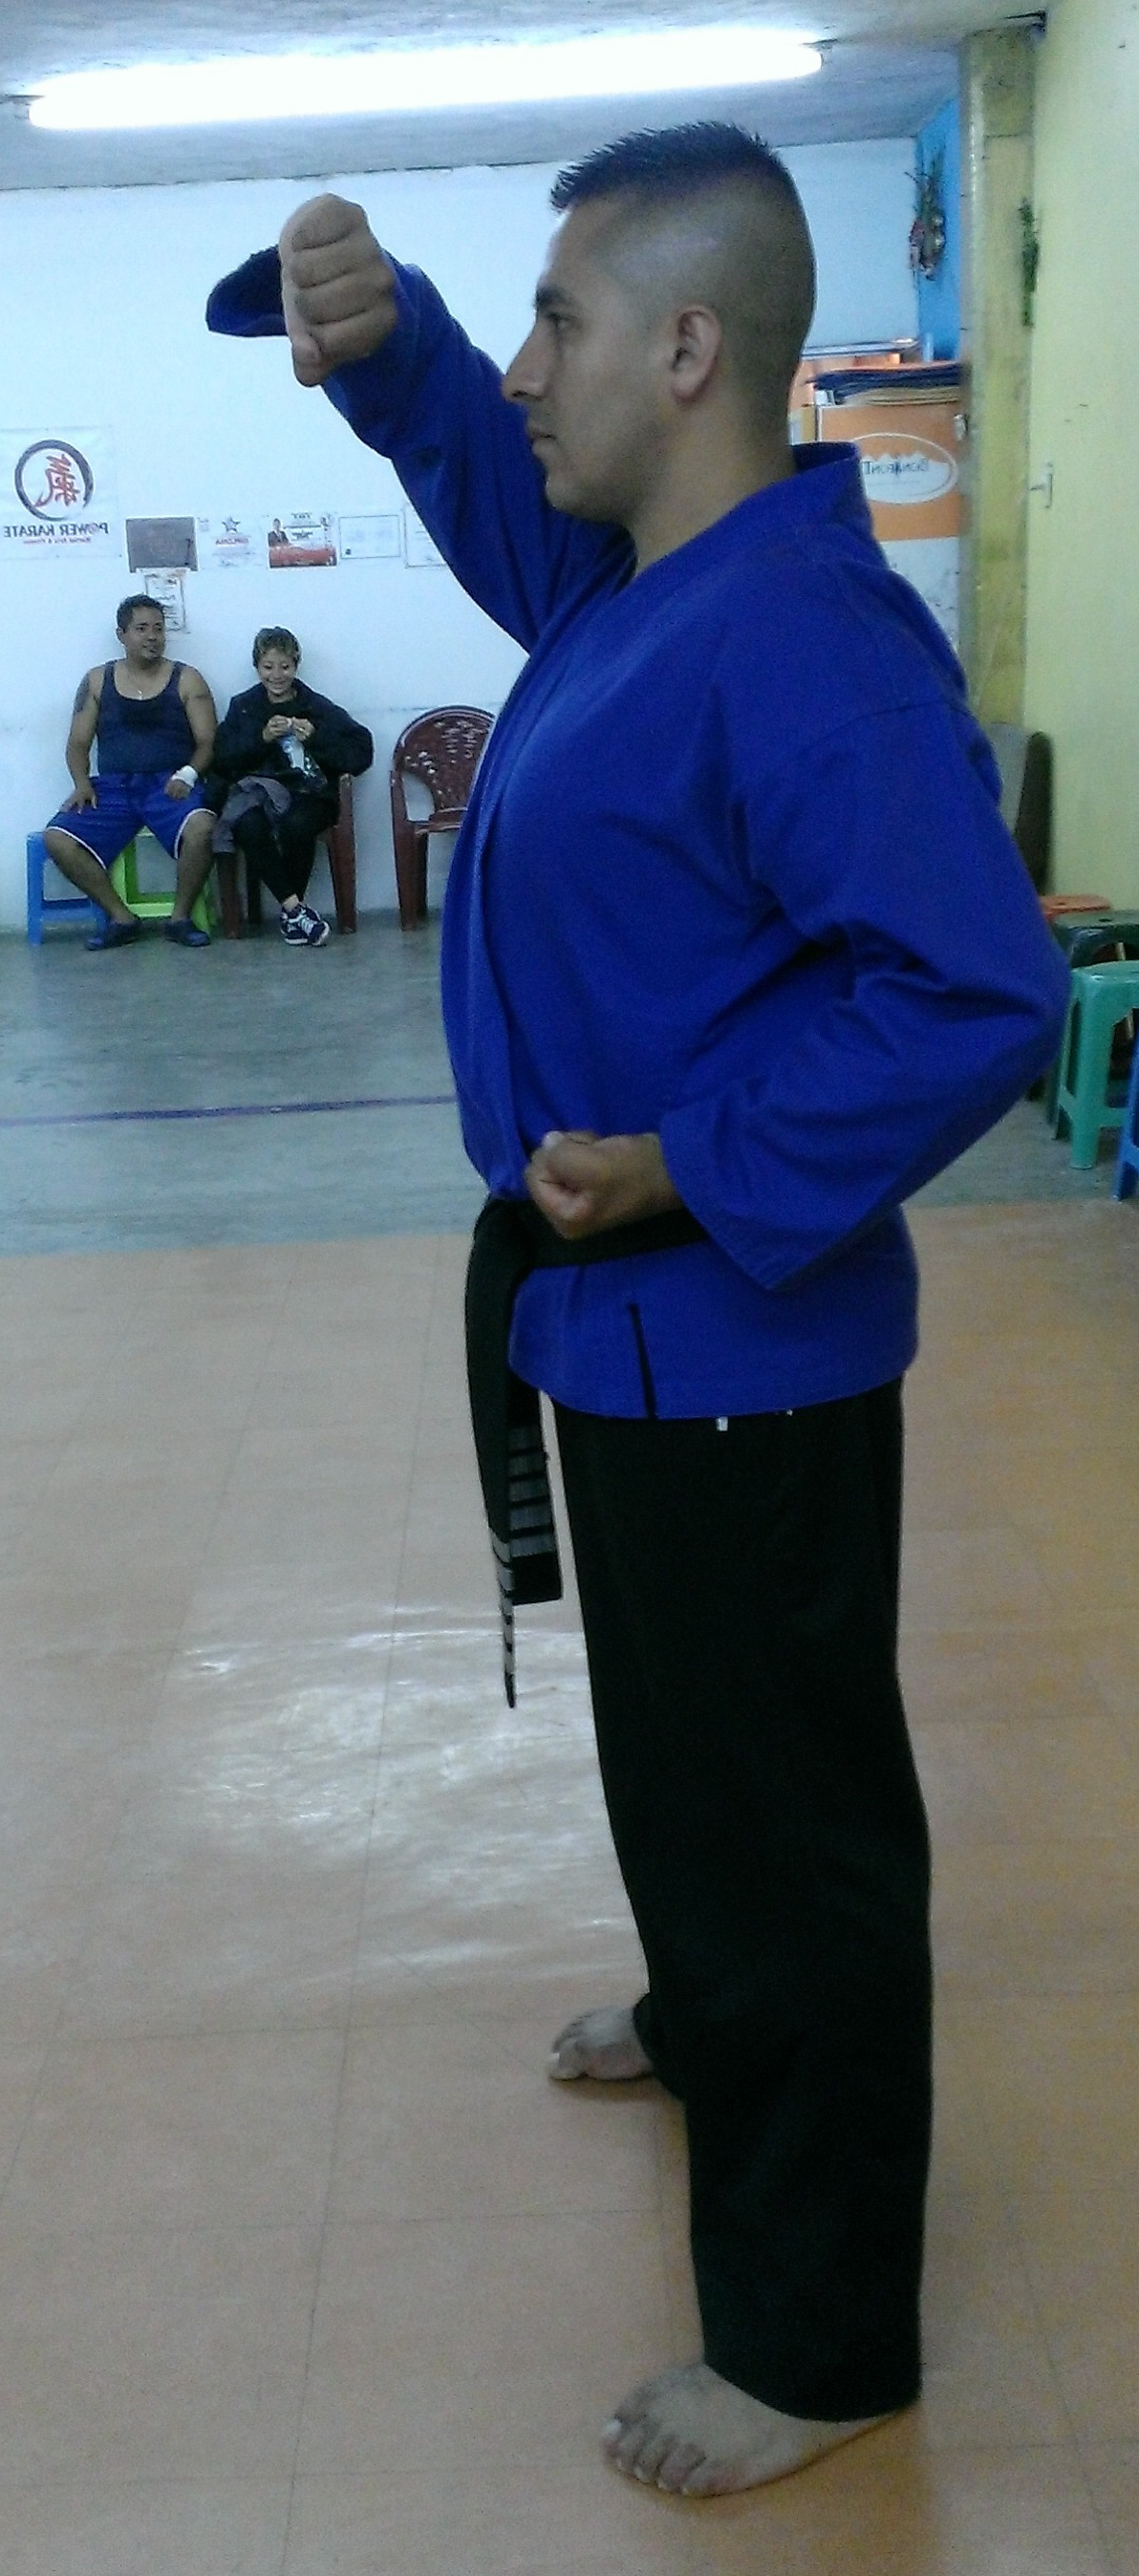
\includegraphics[width=4.5cm, height=8cm]{./Figuras/Tecnica/YodanAgeUke_Lateral}}
	\caption{Defensa Yodan Age Uke}
	\label{fig:Defensas3}
\end{figure}

\begin{figure}[H]
	\centering
	\subfloat[Ataque con brazo Seiken Tsuki frontal]{
		\label{fig:SeikenTsuki_Frontal}
		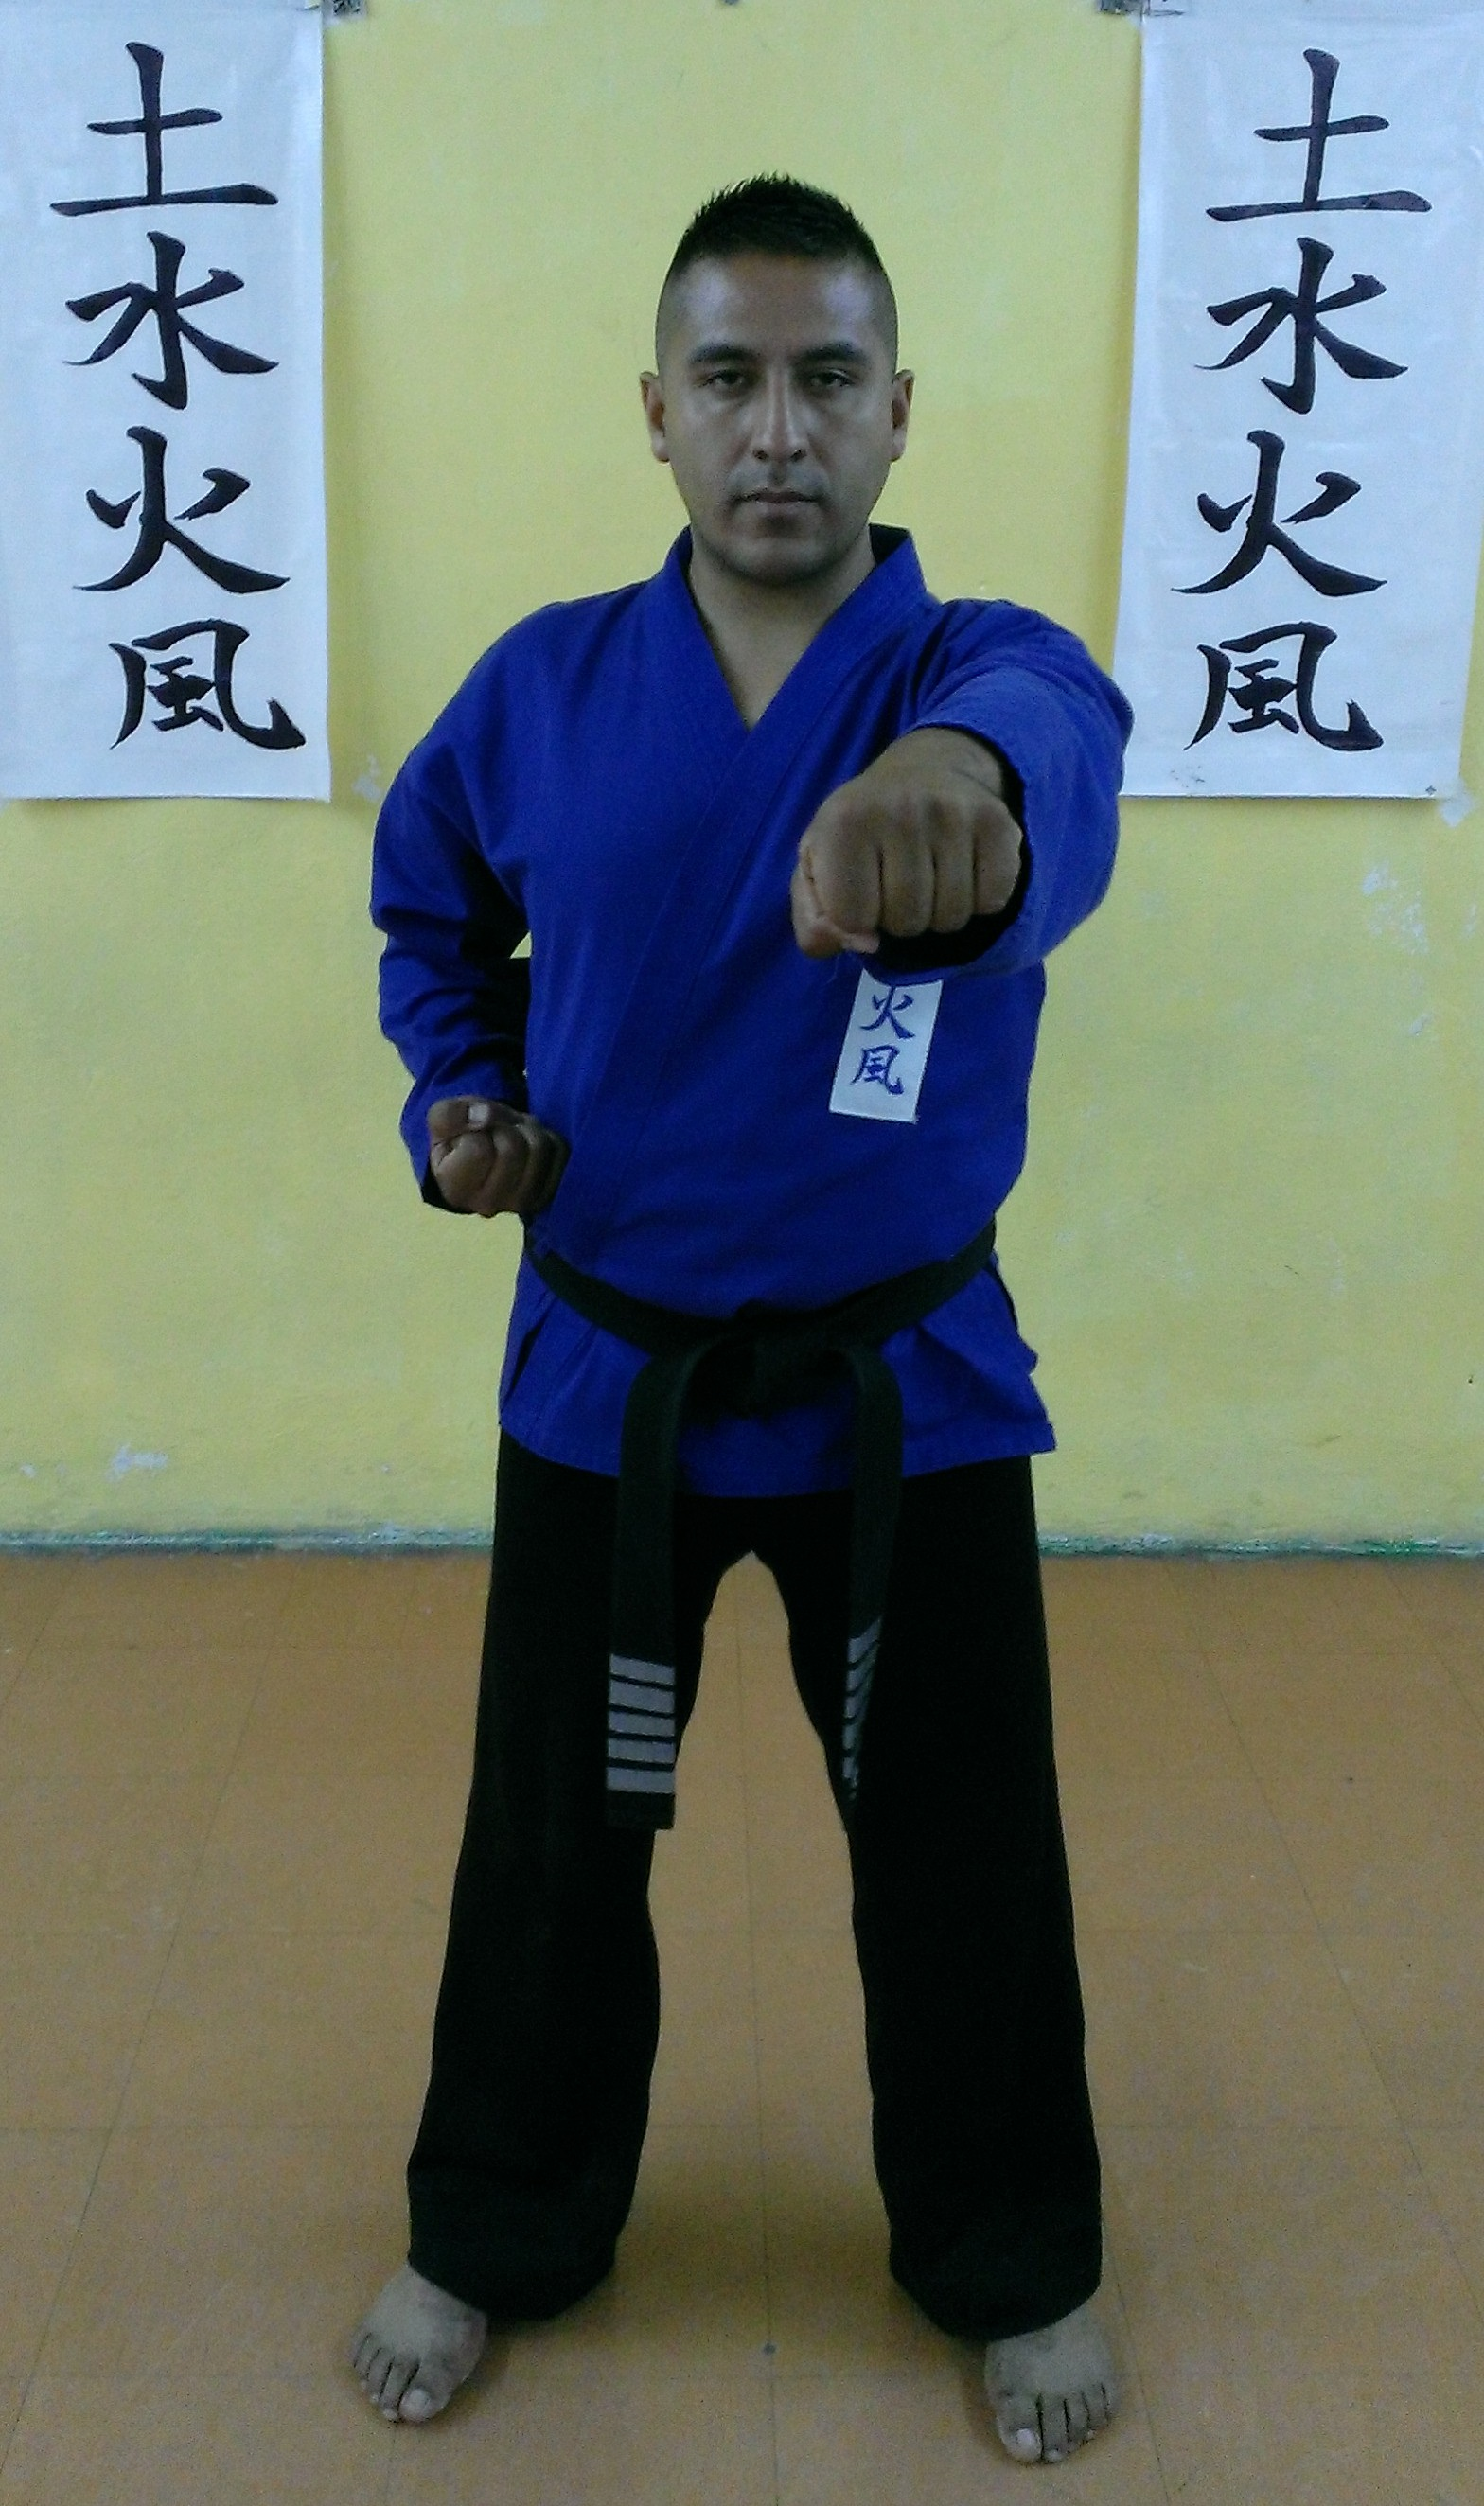
\includegraphics[width=5cm, height=8cm]{./Figuras/Tecnica/SeikenTsuki_Frontal}}
	\subfloat[Ataque con brazo Seiken Tsuki lateral]{
		\label{fig:SeikenTsuki_Lateral}
		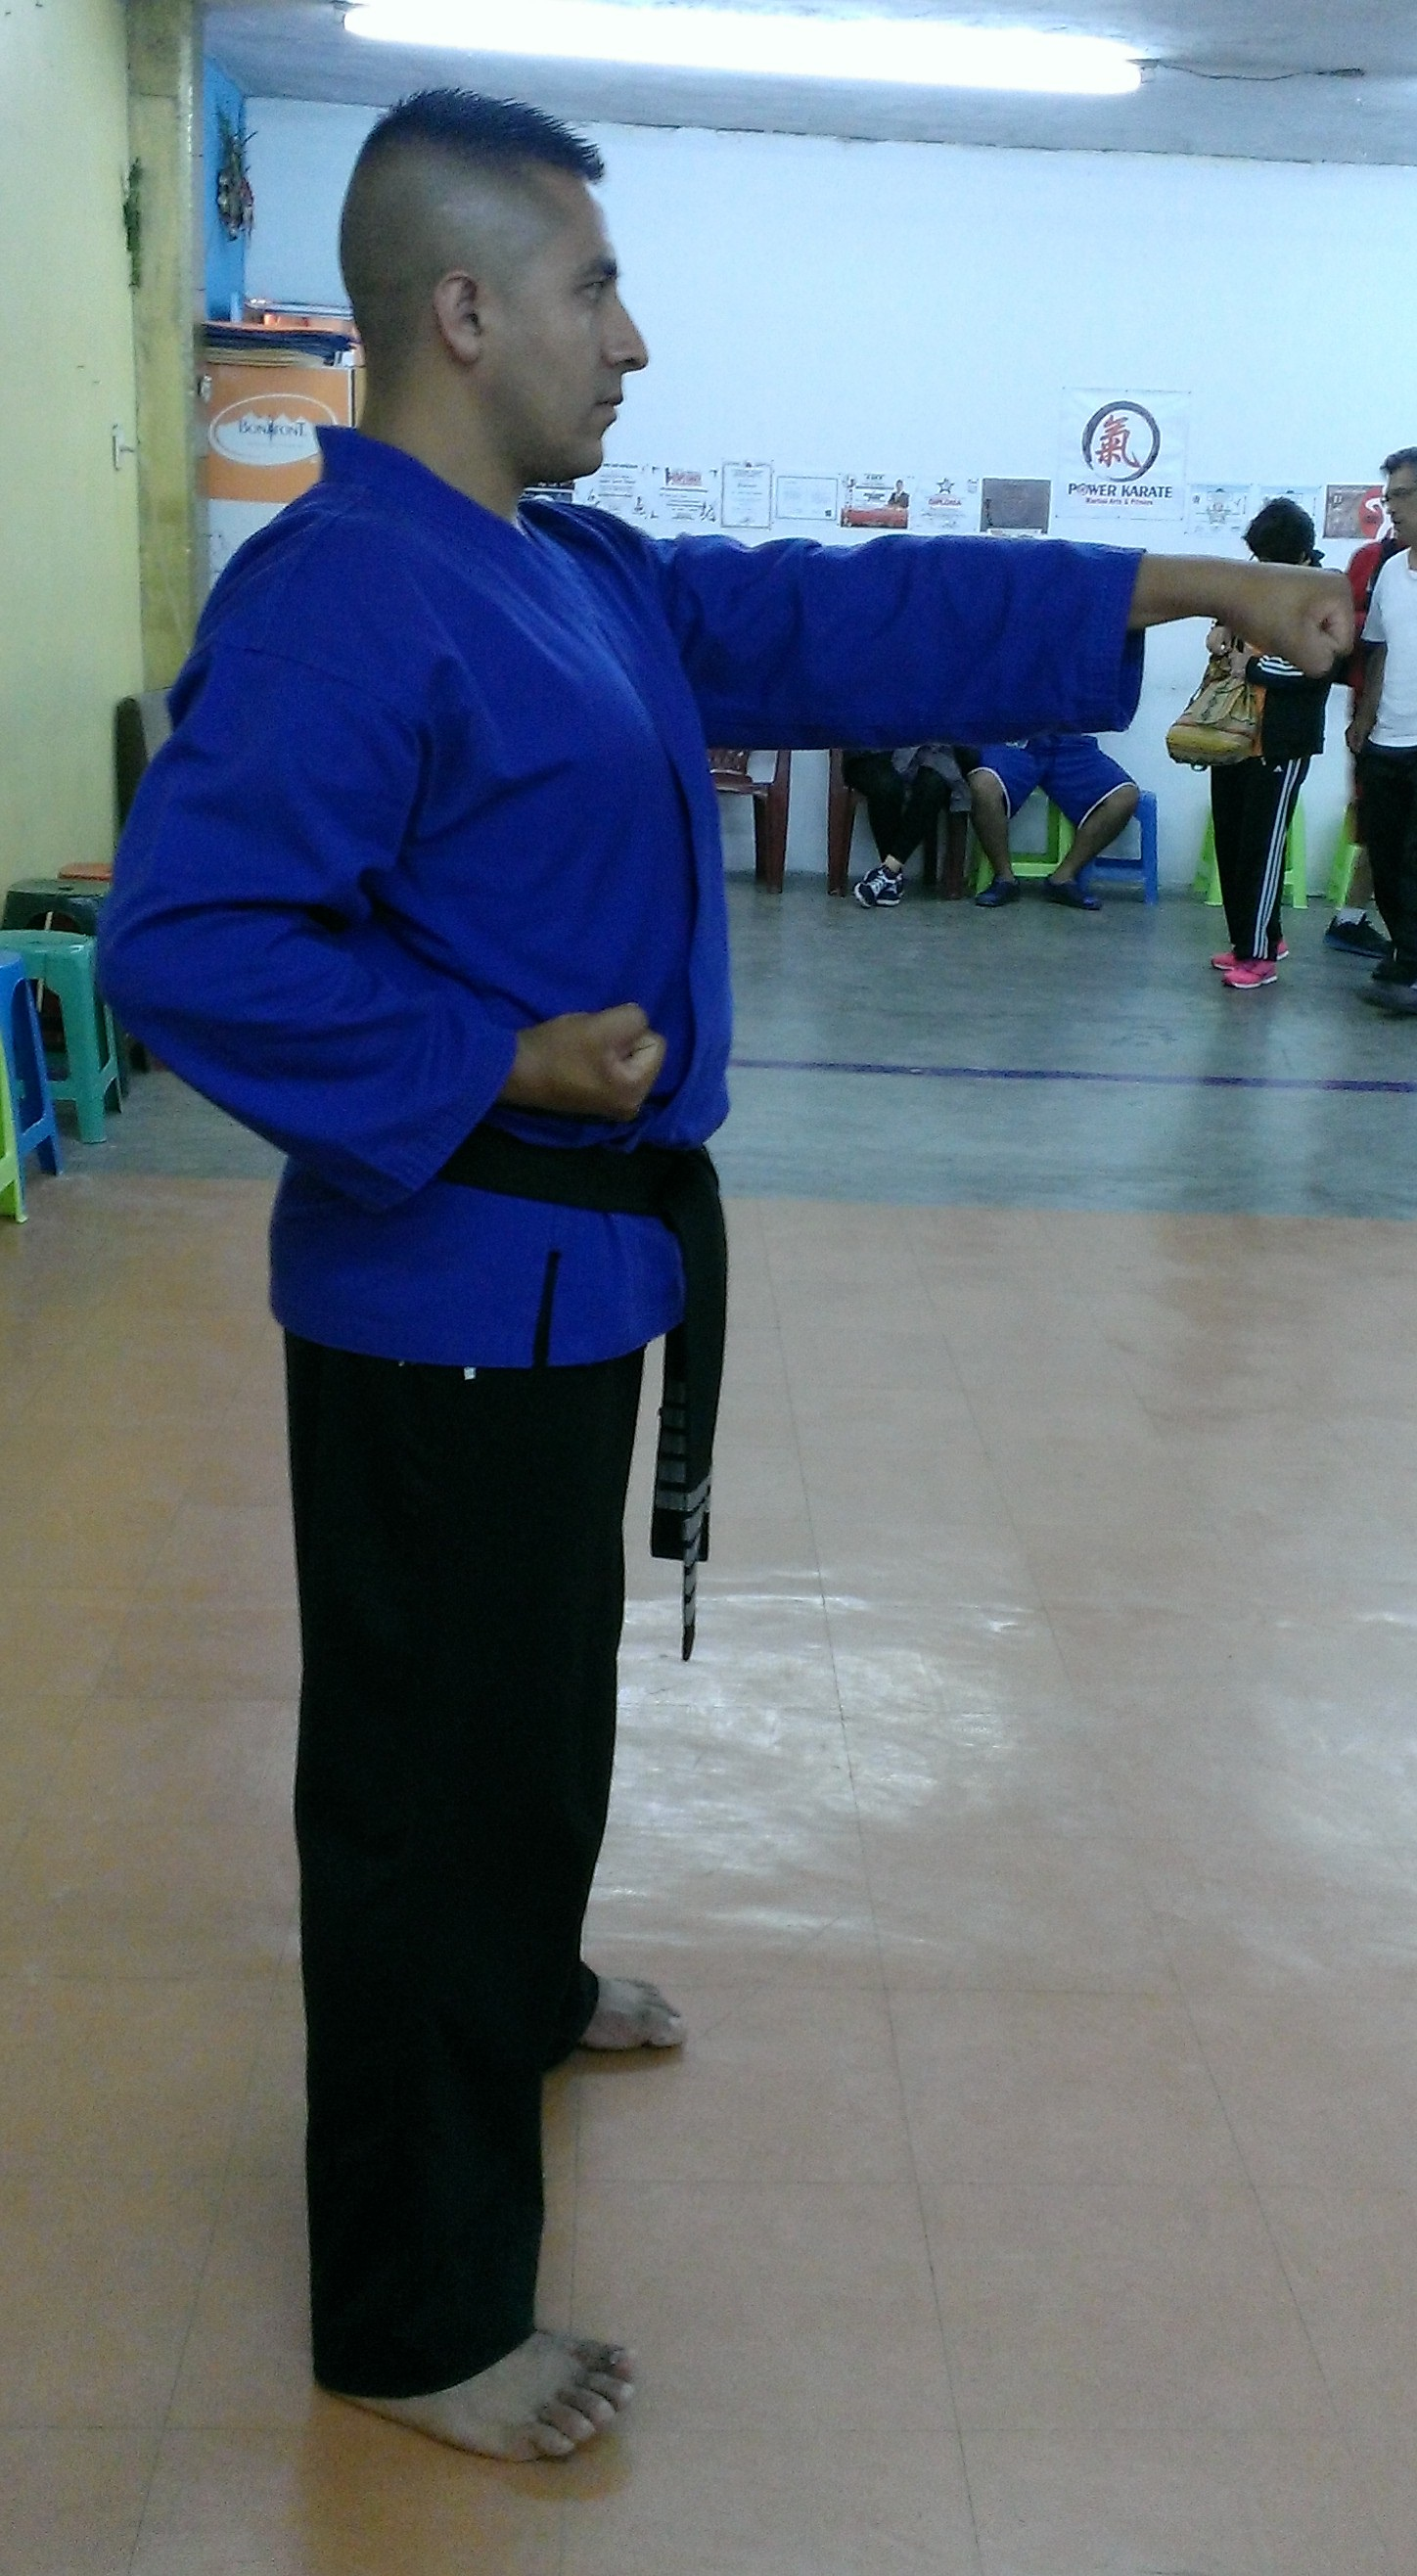
\includegraphics[width=5cm, height=8cm]{./Figuras/Tecnica/SeikenTsuki_Lateral}}
	\caption{Ataque con brazo Seiken Tsuki}
	\label{fig:Ataques1}
\end{figure}

\begin{figure}[H]
	\centering
	\subfloat[Ataque con pierna Mae Geri frontal]{
		\label{fig:MaeGeri_Frontal}
		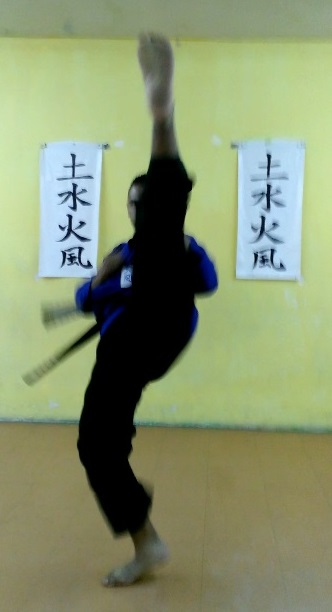
\includegraphics[width=5.5cm, height=8cm]{./Figuras/Tecnica/MaeGeri_Frontal}}
	\subfloat[Ataque con pierna Mae Geri lateral]{
		\label{fig:MaeGeri_Lateral}
		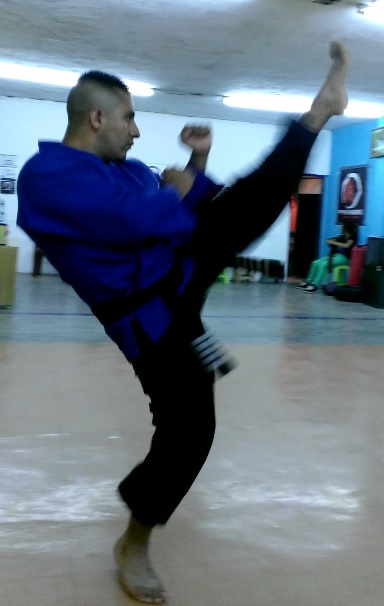
\includegraphics[width=5cm, height=8cm]{./Figuras/Tecnica/MaeGeri_Lateral}}
	\caption{Ataque con pierna Mae Geri}
	\label{fig:Ataques2}
\end{figure}

\clearpage
%-----------------------------------------------------------------------------
\subsubsection{Descripción de movimientos}
La siguiente tabla \ref{tab:DMT} \nameref{tab:DMT} muestra la descripción de los movimientos de técnica, clasificando el tipo de movimiento al que pertenece (posiciones, defensas o ataques).

\begin{table}[H]
\centering
\begin{tabular}{| p{4 cm} | p{2 cm} | p{9 cm} |}
\hline
\rowcolor[rgb]{0.529412, 0.807843, 0.980392} {\textbf{Nombre}} & {\textbf{Tipo}} & {\textbf{Descripción}}\\
\hline
\textbf{Musubi - dachi} &  Posición. & Talones juntos, puntas de los pies separadas, manos a los costados.\\
\hline
\textbf{Hachiji - dachi} &  Posición. & Piernas separadas a la altura de los hombros, puntas de los pies hacia el frente, brazos estirados hacia el frente.\\
\hline
\textbf{Senkuntsu - dachi} &  Posición. & Una pierna flexionando la rodilla y la otra pierna estirada hacia atrás, teniendo una separación entre ellas.\\
\hline
\textbf{Gedan Barai Uke} &  Defensa. & Brazos con los puños cerrados, uno en la cintura y el otro estirado hacia abajo con una separación sobre el cuerpo.\\
\hline
\textbf{Shudan Soto Uke} &  Defensa. & Brazos con los puños cerrados, uno en la cintura y el otro realizando una flexión del codo poniendo el puño a la altura del hombro separados por un espacio entre ellos.\\
\hline
\textbf{Yodan Age Uke} &  Defensa. & Brazos con los puños cerrados, uno en la cintura y el otro realizando una flexión del codo, poniendo el antebrazo a una altura ligeramente mayor a la cabeza.\\
\hline
\textbf{Seiken Tsuki} &  Ataque. & Brazos con los puños cerrados, uno en la cintura y el otro realiza un golpe hacia el frente, a la altura de su pecho.\\
\hline
\textbf{Mae Geri} &  Ataque. & Una pierna apoyada en el sueño y la otra realiza una patada hacia el frente a la altura de su estómago, pecho o cabeza.\\
\hline
\end{tabular}
\caption{Descripción de movimientos de técnica}
\label{tab:DMT}
\end{table} 
%------------------------------------------------------------------------------------
\section{E-Learning}

Con la población en Internet, la demanda de e-Learning ha incrementado recientemente \cite{Chang}. E-Learning representa una aproximación casi ideal para el desarrollo flexible y rentable de competencias desde que pueden ser usadas sin restricciones relacionadas con las ubicaciones físicas y el tiempo de uso \cite{Cukusic}. Una de las principales características del e-Learning es la capacidad de integrar diferentes medios, como texto, imágenes, audio, animaciones y video para crear instrucciones multimedia, promoviendo los intereses de lectura y disposición del aprendiz \cite{Vichuda}. De manera que, la investigación ha mostrado que el diseño de recursos multimedia es costoso y no tienen efectos consistentes en promover el desarrollo del aprendizaje. Por ejemplo, el material didáctico multimedia es menos importante que el proceso y la función del sistema, con el fin de producir un efecto significativo en la comprensión del contenido educativo, aunque de esta forma llame más la atención del aprendiz \cite{Bartscha}. Además, algunas investigaciones muestran que demasiados elementos multimedia innecesarios pueden distraer a los aprendices \cite{Clark}. También, el diseño y desarrollo de recursos multimedia didacticas es costoso, aunque el rapido progreso de las tecnologías de la computación e Internet hacen tal esfuerzo posible \cite{Sun}. No obstante los elementos multimedia son muy importantes para el usuario o aprendiz para utilizar una sistema basado en e-Learning. Por lo tanto, la forma de desarrollar y apoyar los contenidos multimedia efectivos de aprendizaje basadas en el mejor ajuste del alumno de acuerdo con el curso de aprendizaje se está convirtiendo en un problema importante de e-Learning. Con respecto a la evaluación de la evidencia científica, que distribuyen e identifican la calidad del sistema de enseñanza. \\

La educación tradicional en salones de clase no siempre satisface todas las necesidades del nuevo mundo para que el aprendizaje sea permanente. El e-Learning, hace referencia al aprendizaje vía Internet, provee a las personas una forma flexible y personalizada de aprender. Ofrece oportunidades de aprendizaje en demanda y reduce los costos \cite{Zhang}. \\

Enseñar y aprender ya no son exclusivos dentro de un salón de clases tradicional \cite{NC}. Los métodos de aprendizaje necesitan ser más portables y flexibles. El nuevo enfoque del aprendizaje a distancia es construir una infraestructura de costo efectivo que permita el aprendizaje en cualquier tiempo, en cualquier lugar, autodidacta y de forma interactiva.\\

El aprendizaje tradicional cara-a-cara tiene sus ventajas de ser familiar, cercano y confortable tanto para instructores como para estudiantes. Sin embargo, puede requerir viajar e interrumpir el trabajo, causando una pérdida de tiempo. En algunas situaciones, enviar al instructor al lugar puede ser impráctico. El e-Learning sirve como un mecanismo complementario para el aprendizaje remoto o permanente \cite{Zhang}.
%------------------------------------------------------------------------------------
\subsection{E-Learning asíncrono}
\label{sec:elearning}
El e-Learning asíncrono no requiere la participación simultánea de los aprendices e instructores. Se refiere a una situación de aprendizaje donde el evento de aprendizaje no toma lugar en tiempo real \cite{Zhang}. Las personas pueden aprender en cualquier tiempo. Por lo tanto, el e-Learning asíncrono es aprendizaje bajo demanda, lo cual les da a los aprendices más control sobre el proceso del aprendizaje y el contenido.\\

Por las características de este tipo de aprendizaje, se opta por tomar su concepto para ser utilizado en el presente trabajo terminal.
%------------------------------------------------------------------------------------
\subsection{Beneficios del E-Learning}

\begin{itemize}
\item Ahorros de costo y tiempo: Hasta un 40\% del dinero gastado en el aprendizaje individual, es abarcado por el costo del viaje \cite{Zhang}. Desde que los e-Learners no tienen que viajar hasta una locación específica, el e-Learning puede permitir un ahorro en los costos o en gastos indirectos.
\item Aprendizaje autodidacta: El e-Learning fomenta el aprendizaje autodidacta y autodirigido estructurando actividades centradas en el aprendiz. Cada aprendiz puede seleccionar las actividades de aprendizaje  que mejor se adecue a su entorno, intereses y su carrera en ese momento.
\item Ambiente de aprendizaje colaborativo: El e-Learning une a los aprendices y expertos separados físicamente para formar un aprendizaje colaborativo en línea \cite{Hiltz}.
\item Mejor acceso a los instructores: En un ambiente de e-Learning, los aprendices obtienen de los instructores ayuda y orientación en línea.
\end{itemize}

\clearpage
\section{Algoritmo Dynamic Time Warping}
\label{sec:DTW}

Dynamic time warping, es una técnica que encuentra la alineación óptima entre dos series de tiempo, es un algoritmo para medir la similaridad entre dos secuencias, las cuales pueden variar en el tiempo o la velocidad.\\
Puede ser utilizado para encontrar regiones correspondientes entre las dos series o para determinar la similitud entre las dos series de tiempo.\\

Se utiliza a menudo en el reconocimiento de voz para determinar si dos formas de onda representan la misma frase hablada. En una forma de onda del habla, la duración de cada sonido hablado y el intervalo entre sonidos pueden variar, pero las formas de onda del habla deben ser similares.\\
También se ha encontrado útil en muchas otras disciplinas, incluyendo la minería de datos, reconocimiento de gestos, la robótica y la medicina \cite{DTW}.

La distancia euclidiana entre dos series de tiempo no es más que la suma de las distancias cuadradas de cada punto enésimo en una serie de tiempo hasta el punto enésimo en la otra.\\
El principal inconveniente de la utilización de la distancia euclidiana para datos de series de tiempo es que: si dos series de tiempo son idénticas, pero una se desplaza ligeramente a lo largo del eje de tiempo, entonces la distancia euclídea puede considerar que son muy diferentes la una de la otra.\\
DTW se introdujo para superar esta limitación, haciendo caso omiso de los cambios globales y locales en la dimensión de tiempo.\\

En general, el funcionamiento del algoritmo se basa en la búsqueda de un camino óptimo de coincidencia entre dos secuencias con ciertas restricciones. Las secuencias son transformadas no linealmente en el tiempo, de modo que son comprimidas o expandidas en el tiempo para que tengan el mismo largo, y así poder compararlas punto a punto. \\

\textbf{Algoritmo de alineamiento temporal dinámico:} \\

Supongamos que queremos comparar y evaluar la diferencia entre dos señales, supongamos que tenemos dos series de tiempo, un secuencia Q de longitud n, y una secuencia C de longitud m, donde: \\
Q = q1, q2, ..., qi, ..., qn 	(1)\\
C = c1, c2, ..., cj, ... cm 	(2)\\

Para alinear estas dos secuencias utilizando DTW, primero construimos una matriz de n por m,  $d(q_i,c_j) = d(q_i - c_j)^2$, que es la alineación entre los puntos  $q_i$ y $c_j$.\\
Para encontrar la mejor coincidencia entre estas dos secuencias, recuperamos un camino a través de la matriz que minimiza la distancia total acumulada entre ellos, como se ilustra en la Figura. En particular, la ruta óptima es el camino que minimiza el coste.\\

$DTW(Q,C)=min\left\{{\sqrt[]{\sum_{k=1}^K{w_k}}}\right\}$ \\

donde $w_k$ es el elemento de matriz $(i, j)_k$ que también pertenece al k-ésimo elemento de un camino de deformación $W$, un conjunto contiguo de elementos de la matriz que representan un mapeo entre $Q$ y $C$.\\

Este camino se puede encontrar utilizando programación dinámica para evaluar la siguiente repetición.\\
$ \gamma (i, j) = d (q_i, c_j) + min \left\{{\gamma (i-1, j-1), \gamma (i-1, j), \gamma (i, j-1)}\right\} $ \\

donde $d(i, j)$ es la distancia que se encuentra en la celda actual, y $\gamma (i, j)$ es la distancia acumulada de $d (i, j)$ y las distancias acumulativas mínimos de las tres células adyacentes.\\

\begin{figure}[h]%La h significa que la colocara cerca del texto
	\begin{center}
		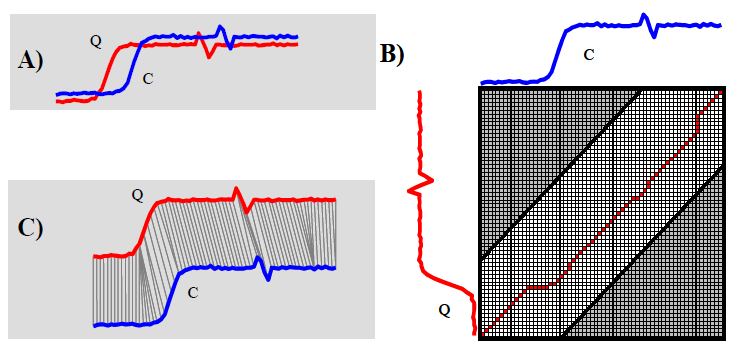
\includegraphics[scale=0.55]{./Figuras/DTWGraficas}
	\end{center}
	\caption{Comparación de dos señales de tiempo con DTW}
	\label{fig:comparacionsenalesdtw}
\end{figure}

La Figura (A) muestra dos secuencias similares Q y C, pero fuera de fase.\\
La Figura (B) para alinear las secuencias, se construye una matriz de deformación y la búsqueda de la ruta óptima, que se muestra con los cuadrados sólidos.\\
La Figura (C) muestra la alineación resultante.\\

Esta secuencia debe satisfacer tres condiciones:\\

1.-Condición de frontera: $p_l=(1,1)$ y $p_L=(N,M)$\\
   Para que los primeros  y los últimos elementos de X e Y estén alineados y así las secuencias completas estén alineadas.\\
   
2.-Condición de monotonía:  $n_1<= n_2<=...n_L $ y $ m_1 <= m_2 <= ... m_L$ \\
   Nos aseguramos de que elementos que se sucedan en el tiempo también se sucedan al ser alineados.\\
   
3.-Condición de salto: Nos indica que no se puede omitir ningún elemento de X e Y y que el camino de alineamiento es continuo.\\

Para reducir el número de rutas a considerar durante el cómputo, varias limitaciones conocidas (condiciones de frontera, la condición de continuidad, condición monótona y Ajuste Ventana Estado) se han aplicado al problema de restringir los movimientos que se pueden hacer desde cualquier punto la ruta de acceso y así restringir el número de caminos que necesitan ser considerados.\\

\clearpage


\chapter{Modelo de procesos de negocio}
El modelo de procesos de negocio es una notación gráfica que describe la lógica de los pasos de un proceso de negocio. Esta notación ha sido especialmente diseñada para coordinar la secuencia de los procesos y los mensajes que fluyen entre los participantes de las diferentes actividades.\\

Los diagramas de procesos de negocio son diagramas diseñados para representar gráficamente la secuencia de todas las actividades que ocurren durante un proceso, basado en la técnica de ``Flow Chart", incluye además toda la información que se considera necesaria para el análisis.\\

La diferencia principal entre el modelado de sistemas en UML y Modelado de procesos de negocio es que se hace más énfasis en como se realiza el trabajo en un organización, en lugar de que trabajo se hace.
%--------------------------------------------------------------------------------------------------------
\section{Modelo actual}
Los siguientes diagramas describen los procesos tradicionales y genéricos que se siguen en un centro educativo para la formación de Karate Do.\\

Documentar ésta información es importante porque es la base del análisis y diseño de nuestro trabajo terminal.\\

\begin{enumerate}
	\item \textbf{Inscripción}\\
	Para realizar el entrenamiento de Karate Do, el Practicante tiene que estar inscrito en una clase. La Figura \ref{fig:PN_Actual_Inscripcion} \nameref{fig:PN_Actual_Inscripcion} muestra el procedimiento a seguir para realizar la inscripción donde el Practicante es quien debe solicitar la inscripción personalmente con el Entrenador y éste a su vez registrar los datos personales del Practicante en una ficha de inscripción.\\
	
	\begin{figure}[H]
		\begin{center}
			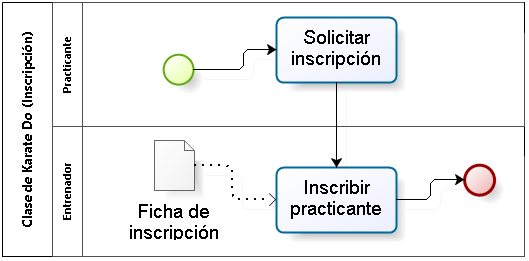
\includegraphics[scale=0.7]{./Figuras/Negocio/Proceso_de_Negocio_actual_inscripcion}
		\end{center}
		\caption{Proceso de negocio actual - Inscripción}
		\label{fig:PN_Actual_Inscripcion}
		%\captionsetup{font={footnotesize,it}}
		%\caption*{Elaboración propia}
	\end{figure}

	\item \textbf{Clase de Karate Do}\\
	Una clase de Karate Do actual consta de 3 partes, el calentamiento, la resistencia y la técnica. La Figura \ref{fig:PN_Actual} \nameref{fig:PN_Actual} muestra el proceso de como se desarrolla una clase de Karate Do.  Para cada una de las partes el Entrenador es quien ejemplifica el ejercicio o movimiento a realizar, después de haber hecho esto, los practicantes replican dicho movimiento y seguido de ello comienzan a realizar repeticiones del mismo. El número de repeticiones del movimiento dependen de lo que el Entrenador establezca. Existen observaciones del Entrenador hacia el Practicante pero no es una tarea que se sigue estrictamente, depende de cada uno de los practicantes y de su desempeño.
	
	\begin{figure}[H]
		\begin{center}
			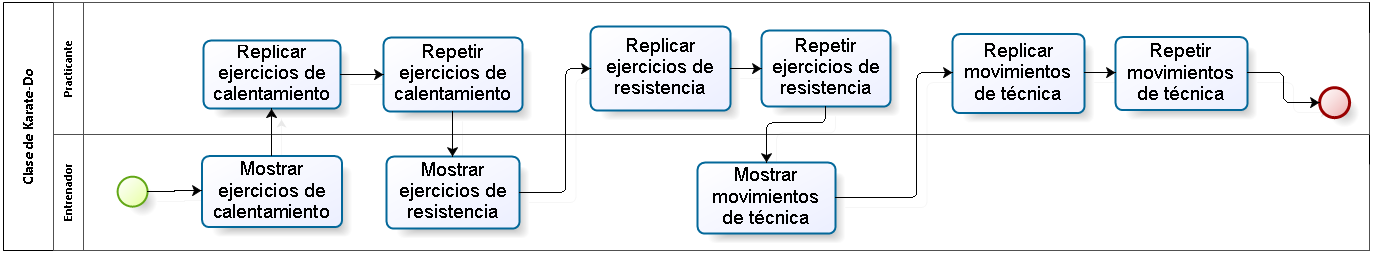
\includegraphics[scale=0.45]{./Figuras/Negocio/Proceso_de_Negocio_actual}
		\end{center}
		\caption{Proceso de negocio actual}
		\label{fig:PN_Actual}
	\end{figure}

\end{enumerate}

%--------------------------------------------------------------------------------------------------------
\section{Modelo propuesto}
El modelo propuesto toma como base el proceso de una clase actual de Karate Do, de donde se toman los ejercicios de calentamiento y los movimientos de técnica delimitados en el \nameref{sec:Alcance} para así desarrollar una herramienta que permita la captura de ejercicios y movimientos para almacenarlos en diferentes rutinas por parte del Entrenador y su posterior replicación por parte de los Practicantes. La Figura \ref{fig:PN_Propuesto} \nameref{fig:PN_Propuesto} muestra la secuencia de acciones que se presenta en el modelo propuesto mediante éste trabajo terminal.\\

\begin{figure}[H]
	\begin{center}
		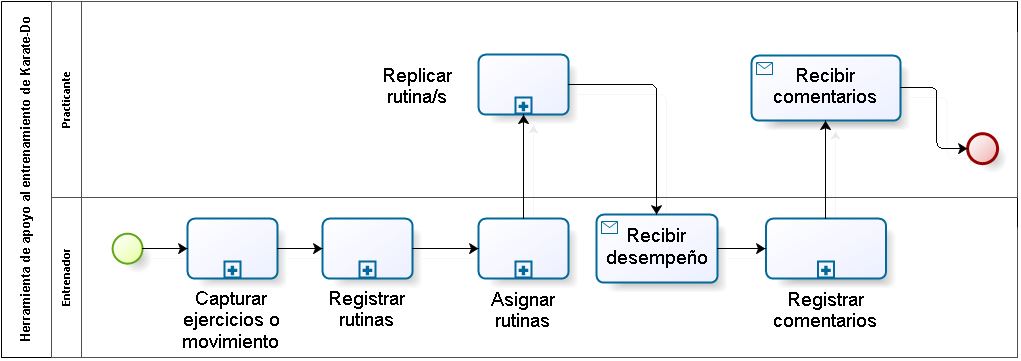
\includegraphics[scale=0.65]{./Figuras/Negocio/Proceso_de_Negocio_propuesto}
	\end{center}
	\caption{Proceso de negocio propuesto}
	\label{fig:PN_Propuesto}
\end{figure}

\begin{enumerate}
	\item \textbf{Registro en la herramienta}\\
	Para poder hacer uso de la herramienta, el Practicante tiene que estar registrado en la misma, para realizar este registro el Practicante lo solicita personalmente al Entrenador y éste escribe los datos personales del Practicante en un formulario de registro de la herramienta tal como lo muestra la Figura \ref{fig:PN_Propuesto_Registro} \nameref{fig:PN_Propuesto_Registro}.\\
	
	\begin{figure}[H]
		\begin{center}
			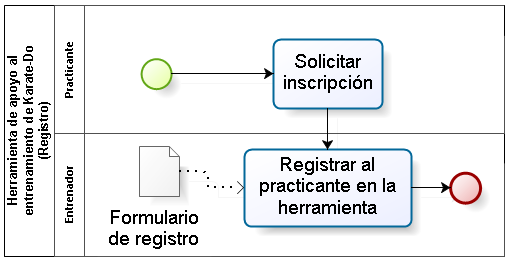
\includegraphics[scale=0.7]{./Figuras/Negocio/Proceso_de_Negocio_propuesto_registro}
		\end{center}
		\caption{Proceso de negocio propuesto - Registro}
		\label{fig:PN_Propuesto_Registro}
	\end{figure}

	\item \textbf{Herramienta de apoyo al entrenamiento de Karate Do}\\
	Para realizar una rutina de entrenamiento a distancia se propone una serie de pasos a realizar dentro de la herramienta los cuales se enlistan a continuación:
	\begin{itemize}
		\item Capturar movimientos (Entrenador): La Figura \ref{fig:procesonegocioP_captEjer} \nameref{fig:procesonegocioP_captEjer} muestra el primer paso para utilizar la herramienta el cual consiste en que el Entrenador capture y guarde los movimientos que utiliza en las rutinas de entrenamiento.
			%Capturar_ejercicios_o_movimientos
			\begin{figure}[H]
				\begin{center}
					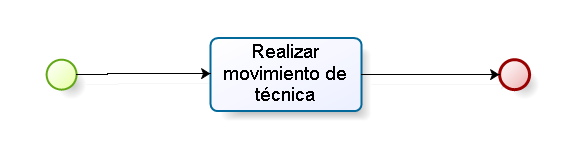
\includegraphics[scale=0.7]{./Figuras/Negocio/Capturar_ejercicios_o_movimientos}
				\end{center}
				\caption{Capturar movimientos}
				\label{fig:procesonegocioP_captEjer}
			\end{figure}
		\item Registrar rutinas (Entrenador): En la Figura \ref{fig:procesonegocioP_regRutinas} \nameref{fig:procesonegocioP_regRutinas} se puede observar que el Entrenador crea las rutinas de acuerdo a su criterio eligiendo de entre los ejercicios de calentamiento y movimientos de técnica que ha capturado previamente.
			%Registrar_rutinas
			\begin{figure}[H]
				\begin{center}
					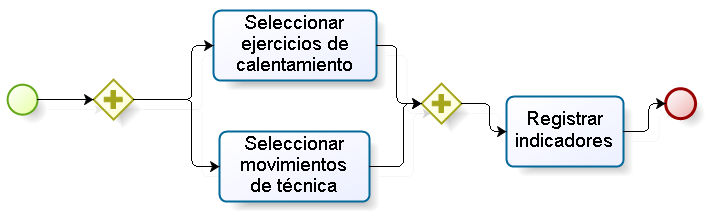
\includegraphics[scale=0.7]{./Figuras/Negocio/Registrar_rutinas}
				\end{center}
				\caption{Registrar rutinas}
				\label{fig:procesonegocioP_regRutinas}
			\end{figure}
		\item Asignar rutinas (Entrenador): Al tener las rutinas registradas, el Entrenador asigna las diferentes rutinas a sus diferentes Practicantes, eligiendo de manera personal las más adecuadas para cada uno de ellos tal como lo muestra la Figura \ref{fig:procesonegocioP_asigRutinas} \nameref{fig:procesonegocioP_asigRutinas}.
			%Asignar Rutinas
			\begin{figure}[H]
				\begin{center}
					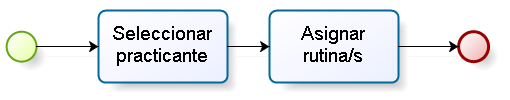
\includegraphics[scale=0.7]{./Figuras/Negocio/Asignar_rutina}
				\end{center}
				\caption{Asignar rutinas}
				\label{fig:procesonegocioP_asigRutinas}
			\end{figure}
		\item Replicar rutinas (Practicante): La Figura \ref{fig:procesonegocioP_repRutinas} \nameref{fig:procesonegocioP_repRutinas} muestra que el trabajo principal del Practicante es la realización de rutinas, es decir replicar los movimientos que el Entrenador le asignó, observando un desempeño final de la rutina el cual además será enviado al Entrenador.
			%Replicar Rutinas
			\begin{figure}[H]
				\begin{center}
					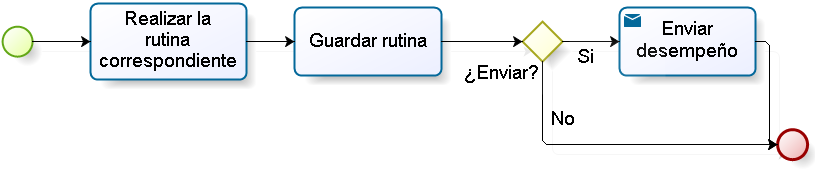
\includegraphics[scale=0.7]{./Figuras/Negocio/Replicar_rutinas}
				\end{center}
				\caption{Replicar rutinas}
				\label{fig:procesonegocioP_repRutinas}
			\end{figure}
		\item Recibir indicadores de desempeño (Entrenador): El Entrenador puede visualizar los resultados del desempeño de cada uno de sus Practicantes.
		\item Registrar comentarios (Entrenador): En base a los resultados previos, el Entrenador puede realizar comentarios en los cuales puede ingresar sugerencias u observaciones para el Practicante, tal como se puede observar en la Figura \ref{fig:procesonegocioP_regComent} \nameref{fig:procesonegocioP_regComent}.
			%Registrar comentarios
			\begin{figure}[H]
				\begin{center}
					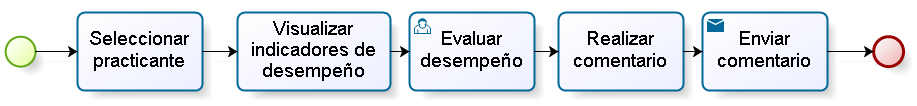
\includegraphics[scale=0.7]{./Figuras/Negocio/Registrar_comentarios}
				\end{center}
				\caption{Registrar comentarios}
				\label{fig:procesonegocioP_regComent}
		\end{figure}
		\item Recibir comentarios (Practicante): El Practicante puede visualizar los comentarios hechos por el Entrenador, para poder hacer las mejoras pertinentes y en la próxima rutina mejorar su desempeño.
	\end{itemize}
	
\end{enumerate}
\clearpage
\chapter{Análisis de requerimientos}
En el presente capítulo se realiza el análisis correspondiente para la obtención de los requerimientos de la herramienta, comenzando por la definición de los actores participantes y el alcance planteado, obteniendo así el listado de los requerimientos y las reglas de negocio.
%------------------------------------------------------------------------------------
\section{Definición de actores}
En la presente sección se realiza la especificación de los actores que tendrán interacción con la Herramienta de Apoyo al Entrenamiento de Karate Do. A continuación se describen los actores de acuerdo a las actividades que desarrollan.
%------------------------------------------------------------------------------------
\subsection{Entrenador}
\label{act:Entrenador} 
\textbf{\textcolor[rgb]{0, 0, 0.545098}{Nombre:}} Entrenador \\

\textbf{\textcolor[rgb]{0, 0, 0.545098}{Descripción:}} Persona experta en el arte marcial del Karate Do, la cual domina todos los movimientos de técnica y ejercicios de una rutina de entrenamiento, además de llevar un seguimiento del desempeño de cada uno de sus aprendices. \\

\textbf{\textcolor[rgb]{0, 0, 0.545098}{Responsabilidades:}}
\begin{itemize}
	\item Registrar a los practicantes en la herramienta.
	\item Registrar movimientos de técnica. 
	\item Registrar rutinas de entrenamiento.
	\item Visualizar la información de registro de los practicantes.
	\item Visualizar la lista de los ejercicios de calentamiento.
	\item Visualizar la lista de los movimientos de técnica.
	\item Visualizar la lista de las rutinas de entrenamiento.
	\item Visualizar la trayectoria del desempeño de los practicantes.
	\item Modificar la información de registro de los practicantes.
	\item Modificar los identificadores de las rutinas de entrenamiento.
	\item Asignar a los practicantes una rutina.
	\item Realizar comentarios sobre el desempeño de cada Practicante.
\end{itemize}
\vspace{1em}

\textbf{\textcolor[rgb]{0, 0, 0.545098}{Perfil:}}
\begin{itemize}
	\item Contar con un grado de al menos cinta negra primer Dan.
	\item Conocimientos en el uso de computadora.
	\item Conocimientos básicos en el uso del sensor Kinect.
\end{itemize}
\vspace{1em}

\textbf{\textcolor[rgb]{0, 0, 0.545098}{Cantidad:}} Uno.
%------------------------------------------------------------------------------------
\subsection{Practicante}
\label{act:Practicante}
\textbf{\textcolor[rgb]{0, 0, 0.545098}{Nombre:}} Practicante. \\

\textbf{\textcolor[rgb]{0, 0, 0.545098}{Descripción:}} Aprendiz de Karate Do cuyo principal interés es aprender nuevas técnicas o mejorar sus habilidades en dicho arte marcial, la cual entrena y realiza las rutinas de entrenamiento registradas por un Entrenador experto. \\

\textbf{\textcolor[rgb]{0, 0, 0.545098}{Responsabilidades:}}
\begin{itemize}
	\item Visualizar las rutinas de entrenamiento asignadas por el Entrenador.
	\item Visualizar los comentarios realizados por su Entrenador.
	\item Visualizar su información de registro.
	\item Modificar la contraseña de inicio de sesión en la herramienta.
	\item Replicar los ejercicios de calentamiento de una rutina seleccionada.
	\item Replicar los movimientos de técnica de una rutina seleccionada.
	\item Enviar la rutina de entrenamiento replicada.
\end{itemize}
\vspace{1em}

\clearpage

\textbf{\textcolor[rgb]{0, 0, 0.545098}{Perfil:}}
\begin{itemize}
	\item Gozar de buena salud y no padecer una enfermedad que se vea afectada por el esfuerzo físico.
	\item No contar con alguna discapacidad física que impida realizar los movimientos propuestos por la herramienta. 
	\item Conocimientos en el uso de una computadora.
	\item Conocimientos básicos en el uso del sensor Kinect.
	%*\item Estatura 
\end{itemize}
\vspace{1em}

\textbf{\textcolor[rgb]{0, 0, 0.545098}{Cantidad:}} De uno a diez, cada uno con una sesión independiente.
%------------------------------------------------------------------------------------
\section{Alcance}
\label{sec:Alcance}
\textbf{El alcance de esta herramienta contempla los siguientes puntos:}\\
\begin{enumerate}
	\item \textbf{\textcolor[rgb]{0, 0, 0.545098}{Un Entrenador.}}\\
	El presente trabajo terminal está planteado como una herramienta de apoyo al entrenamiento de Karate Do, es decir estamos transportando parte de una clase de entrenamiento, a un entrenamiento a distancia, y una clase normal consiste en un solo Entrenador dando instrucciones a un grupo de practicantes.\\
	\item \textbf{\textcolor[rgb]{0, 0, 0.545098}{De 1 a 10 practicantes, cada uno con una sesión independiente.}}\\
	En base a una encuesta realizada (véase anexo \ref{anex:encuesta} \nameref{anex:encuesta}), determinamos que lo ideal para un grupo de entrenamiento de Karate Do (una clase) es tener a 10 practicantes. Se propone de manera no simultánea ya que al ser una herramienta de apoyo, damos la libertad de que cada Practicante realice sus rutinas en el tiempo en que cada uno de ellos tenga la posibilidad, y no forzamos un horario determinado.\\
	\item \textbf{\textcolor[rgb]{0, 0, 0.545098}{Ejercicios de calentamiento y técnica.}}\\
	Un entrenamiento completo de Karate Do contempla ejercicios de calentamiento, ejercicios de resistencia y técnica (la cual a su vez se divide en movimientos, combate y katas); para el presente trabajo tomamos en cuenta sólo los ejercicios de calentamiento y los movimientos de técnica inicial ya que se trata de un apoyo al entrenamiento, pues los movimientos de técnica  requieren de un aprendizaje y un entrenamiento constante para mejorar esas habilidades, y para realizar los movimientos de técnica es necesario realizar un calentamiento previo, ya que aunque son movimientos, se requiere un esfuerzo físico e incluso de estiramiento de extremidades.\\
	\item \textbf{\textcolor[rgb]{0, 0, 0.545098}{10 ejercicios de calentamiento disponibles en total.}}\\
	Se proponen al menos 1 ejercicio de calentamiento por cada parte del cuerpo importante para realizar los movimientos de técnica y el uso o la selección de alguno de ellos dependerá del tipo de rutina que el Entrenador vaya a asignar.\\
	\item \textbf{\textcolor[rgb]{0, 0, 0.545098}{8 movimientos de técnica disponibles en total (2 ataques, 3 defensas y 3 posiciones).}}\\
	Se proponen los movimientos de técnica básicos correspondientes a la cinta blanca, el uso de cada uno de ellos dependerá del tipo de rutina que el Entrenador vaya a asignar.\\
	\item \textbf{\textcolor[rgb]{0, 0, 0.545098}{24 rutinas de entrenamiento registradas.}}\\
	De acuerdo a la encuesta realizada (véase \ref{anex:encuesta} \nameref{anex:encuesta}), determinamos que el número de clases ideal para el entrenamiento de Karate Do es de 3 por semana, en este trabajo se propone de esa manera 3 rutinas de entrenamiento por semana, y dado que el entrenamiento completo para poder realizar un examen y cambiar a cinta blanca es de 2 meses, se determina que el número total de rutinas que el Entrenador puede registrar como máximo es de 24.\\
	\item \textbf{\textcolor[rgb]{0, 0, 0.545098}{E-Learning asíncrono.}}\\
	Como se describe en el marco teórico en la sección \ref{sec:elearning} \nameref{sec:elearning}, el e-Learning asíncrono hace referencia a un aprendizaje en el que el profesor y el alumno no tienen que estar conectados al mismo tiempo, pero en el cual sigue existiendo un seguimiento y apoyo de dicho profesor hacia el alumno.\\
	\item \textbf{\textcolor[rgb]{0, 0, 0.545098}{Dos Interfaces Naturales de Usuario.}}\\
	Ambas aplicaciones contarán con una Interfaz Natural de UsuarioLa interfaz del Entrenador será una INU en las partes de de captura y validación de movimientos.\\
	

\end{enumerate}
\vspace{1em}
\textbf{La herramienta no contempla los siguientes puntos (posible trabajo a futuro):}\\

\begin{enumerate}
	\item \textbf{\textcolor[rgb]{0, 0, 0.545098}{Más de un Entrenador, es decir, una organización completa.}}\\
	Como se mencionó previamente, la herramienta está propuesta para apoyar el entrenamiento de una clase de Karate Do, por lo que el manejo de diferentes entrenadores, o una organización completa queda fuera de nuestros objetivos.\\
	\item \textbf{\textcolor[rgb]{0, 0, 0.545098}{Ejercicios de resistencia, entrenamiento de combate y katas.}}\\
	Los ejercicios de resistencia, son ejercicios que requieren de un esfuerzo físico mayor y que en diversas ocasiones no es necesario replicar algún movimiento de manera exacta, ya que para estos se requieren de otros factores como la condición física del Practicante o su complexión por mencionar algunos ejemplos.\\
El entrenamiento del combate requiere de otro Practicante para que se lleve a cabo de manera adecuada, además de un área de entrenamiento mayor ya que existen desplazamientos no uniformes cuando se realiza.\\
El entrenamiento de katas requiere de desplazamientos lineales horizontales y verticales por lo que estas validaciones quedan fuera de los objetivos principales.\\
	\item \textbf{\textcolor[rgb]{0, 0, 0.545098}{E-Learning síncrono.}}\\
	El e-Learning síncrono hace referencia al aprendizaje en el cual el profesor y el alumno se encuentran comunicados en tiempo real, como si se tratase de una clase en persona; como se mencionó previamente este trabajo es un apoyo y si eligiéramos este tipo de aprendizaje, tendríamos que restringir la realización de las rutinas a un horario determinado y entraría en conflicto con los objetivos y justificaciones propuestos.\\
	\item \textbf{\textcolor[rgb]{0, 0, 0.545098}{Uso de streaming.}}\\
	El uso de video en streaming requiere una cantidad significativa de ancho de banda de ambas partes de la herramienta para que la calidad de imagen sea favorable; en el presente trabajo se requiere que la herramienta funcione de manera adecuada sin necesidad de tener una conexión de alta velocidad.\\
	\item \textbf{\textcolor[rgb]{0, 0, 0.545098}{Grabación de video.}}\\
	La transferencia directa de archivos no está contemplada por el tipo de e-Learning, además de que la transferencia (subida y bajada) de archivos de video es costosa respecto al ancho de banda.\\
\end{enumerate}
\clearpage
%------------------------------------------------------------------------------------
\section{Requerimientos funcionales}

Los requerimientos funcionales se han abordado respecto a lo que se espera que la herramienta cubra en funcionalidad para el entrenamiento de la técnica inicial de cinta blanca del Karate Do. A continuación se muestra cada uno de los requerimientos identificados en el módulo Entrenador y en el módulo Practicante, especificando para cada uno de ellos un identificador único con el cual se hará referencia a los mismos en el documento, el nombre del requerimiento y su descripción. \\

%--------------------------------------------------------------------------------------------------------
\subsection{Requerimientos funcionales aplicación Entrenador}

\textbf{\textcolor[rgb]{0, 0, 0.545098}{RF01-E \hspace{2cm} Registro de practicantes}}\\
\rule[3mm]{17cm}{0.1mm}
\label{rf:RF01-E}
\textbf{Descripción: } Podrá realizar el registro de cada Practicante ingresando la información correspondiente al formulario de registro (ver \nameref{rn:RNR01} ). \\
\textbf{Versión: } 2. \\

\textbf{\textcolor[rgb]{0, 0, 0.545098}{RF02-E \hspace{2cm} Generación de contraseñas}}\\
\rule[3mm]{17cm}{0.1mm}
\label{rf:RF02-E}
\textbf{Descripción: } La contraseña del Practicante será generada automáticamente por la herramienta y será enviada al correo electrónico previamente registrado. \\
\textbf{Versión: } 2. \\

\textbf{\textcolor[rgb]{0, 0, 0.545098}{RF03-E \hspace{2cm} Consulta de información de los practicantes}}\\
\rule[3mm]{17cm}{0.1mm}
\label{rf:RF03-E}
\textbf{Descripción: } Podrá visualizar la lista de practicantes registrados además de su información personal. \\
\textbf{Versión: } 2. \\

\textbf{\textcolor[rgb]{0, 0, 0.545098}{RF04-E \hspace{2cm} Modificación de información de los practicantes}}\\
\rule[3mm]{17cm}{0.1mm}
\label{rf:RF04-E}
\textbf{Descripción: } Podrá realizar modificaciones en la información personal de los practicantes. \\
\textbf{Versión: } 2. \\

\textbf{\textcolor[rgb]{0, 0, 0.545098}{RF05-E \hspace{2cm} Consulta de trayectoria del Practicante}}\\
\rule[3mm]{17cm}{0.1mm}
\label{rf:RF05-E}
\textbf{Descripción: } Podrá visualizar el desempeño del Practicante. \\
\textbf{Versión: } 2. \\

\textbf{\textcolor[rgb]{0, 0, 0.545098}{RF06-E \hspace{2cm} Baja de Practicante}}\\
\rule[3mm]{17cm}{0.1mm}
\label{rf:RF06-E}
\textbf{Descripción: } Deberá tener la opción para poder dar de baja algún Practicante previamente registrado. \\
\textbf{Versión: } 2. \\

\textbf{\textcolor[rgb]{0, 0, 0.545098}{RF07-E \hspace{2cm} Captura de movimientos de técnica}}\\
\rule[3mm]{17cm}{0.1mm}
\label{rf:RF07-E}
\textbf{Descripción: } Podrá realizar la captura de movimientos de técnica. \\
\textbf{Versión: } 2. \\

\textbf{\textcolor[rgb]{0, 0, 0.545098}{RF08-E \hspace{2cm} Registro de rutinas de entrenamiento}}\\
\rule[3mm]{17cm}{0.1mm}
\label{rf:RF08-E}
\textbf{Descripción: } Podrá realizar el registro de rutinas de entrenamiento seleccionando los ejercicios de un catálogo y movimientos previamente capturados. \\
\textbf{Versión: } 2. \\

\textbf{\textcolor[rgb]{0, 0, 0.545098}{RF09-E \hspace{2cm} Modificación de identificadores de rutinas de entrenamiento}}\\
\rule[3mm]{17cm}{0.1mm}
\label{rf:RF09-E}
\textbf{Descripción: } Podrá realizar modificaciones en los identificadores de las rutinas de entrenamiento. \\
\textbf{Versión: } 2. \\

\textbf{\textcolor[rgb]{0, 0, 0.545098}{RF10-E \hspace{2cm} Baja de rutinas de entrenamiento}}\\
\rule[3mm]{17cm}{0.1mm}
\label{rf:RF10-E}
\textbf{Descripción: } Deberá tener la opción para poder dar de baja alguna rutina de entrenamiento. \\
\textbf{Versión: } 2. \\

\textbf{\textcolor[rgb]{0, 0, 0.545098}{RF11-E \hspace{2cm} Consulta del resultado del desempeño de las rutinas.}}\\
\rule[3mm]{17cm}{0.1mm}
\label{rf:RF11-E}
\textbf{Descripción: } Podrá visualizar el resultado del desempeño que la herramienta generará de forma porcentual con respecto a la exactitud de cada movimiento de técnica, en la rutina que el Practicante realizó. \\
\textbf{Versión: } 2. \\

\textbf{\textcolor[rgb]{0, 0, 0.545098}{RF12-E \hspace{2cm} Registro de comentarios de rutinas}}\\
\rule[3mm]{17cm}{0.1mm}
\label{rf:RF12-E}
\textbf{Descripción: } Podrá realizar comentarios escritos a la rutina realizada por el Practicante. \\
\textbf{Versión: } 2. \\

\textbf{\textcolor[rgb]{0, 0, 0.545098}{RF13-E \hspace{2cm} Modificación de comentarios}}\\
\rule[3mm]{17cm}{0.1mm}
\label{rf:RF13-E}
\textbf{Descripción: } Tendrá la opción para poder modificar los comentarios. \\
\textbf{Versión: } 2. \\
%--------------------------------------------------------------------------------------------------------

\subsection{Requerimientos funcionales aplicación Practicante}

\textbf{\textcolor[rgb]{0, 0, 0.545098}{RF01-P \hspace{2cm} Inicio de sesión del Practicante}}\\
\rule[3mm]{17cm}{0.1mm}
\label{rf:RF01-P}
\textbf{Descripción: } Podrá entrar a la herramienta, ingresando el nombre de usuario y contraseña previamente asignados. \\
\textbf{Versión: } 2. \\

\textbf{\textcolor[rgb]{0, 0, 0.545098}{RF02-P \hspace{2cm} Recuperar contraseña}}\\
\rule[3mm]{17cm}{0.1mm}
\label{rf:RF02-P}
\textbf{Descripción: } Podrá solicitar la recuperación de su contraseña. \\
\textbf{Versión: } 2. \\

\textbf{\textcolor[rgb]{0, 0, 0.545098}{RF03-P \hspace{2cm} Modificar contraseña}}\\
\rule[3mm]{17cm}{0.1mm}
\label{rf:RF03-P}
\textbf{Descripción: } Podrá modificar su contraseña actual. \\
\textbf{Versión: } 2. \\

\textbf{\textcolor[rgb]{0, 0, 0.545098}{RF04-P \hspace{2cm} Consulta de información del Practicante}}\\
\rule[3mm]{17cm}{0.1mm}
\label{rf:RF04-P}
\textbf{Descripción: } Podrá visualizar la información contenida en su registro. \\
\textbf{Versión: } 2. \\

\textbf{\textcolor[rgb]{0, 0, 0.545098}{RF05-P \hspace{2cm} Visualizar rutina de entrenamiento}}\\
\rule[3mm]{17cm}{0.1mm}
\label{rf:RF05-P}
\textbf{Descripción: } Podrá visualizar las rutinas asignadas por el Entrenador. \\
\textbf{Versión: } 2. \\

\textbf{\textcolor[rgb]{0, 0, 0.545098}{RF06-P \hspace{2cm} Seleccionar rutina de entrenamiento}}\\
\rule[3mm]{17cm}{0.1mm}
\label{rf:RF06-P}
\textbf{Descripción: } Podrá seleccionar la rutina de entrenamiento asignada por el Entrenador. \\
\textbf{Versión: } 2. \\

\textbf{\textcolor[rgb]{0, 0, 0.545098}{RF07-P \hspace{2cm} Realizar movimientos}}\\
\rule[3mm]{17cm}{0.1mm}
\label{rf:RF07-P}
\textbf{Descripción: } La herramienta identificará los movimientos que el Practicante ha replicado. \\
\textbf{Versión: } 2. \\

\textbf{\textcolor[rgb]{0, 0, 0.545098}{RF08-P \hspace{2cm} Repetir rutina de entrenamiento}}\\
\rule[3mm]{17cm}{0.1mm}
\label{rf:RF08-P}
\textbf{Descripción: } Deberá tener la opción de repetir la rutina de entrenamiento antes de enviarla al Entrenador. \\
\textbf{Versión: } 2. \\

\textbf{\textcolor[rgb]{0, 0, 0.545098}{RF09-P \hspace{2cm} Guardar rutina de entrenamiento}}\\
\rule[3mm]{17cm}{0.1mm}
\label{rf:RF09-P}
\textbf{Descripción: } Deberá poder guardar la rutina de entrenamiento realizada. \\
\textbf{Versión: } 2. \\

\textbf{\textcolor[rgb]{0, 0, 0.545098}{RF10-P \hspace{2cm} Enviar desempeño de rutina}}\\
\rule[3mm]{17cm}{0.1mm}
\label{rf:RF10-P}
\textbf{Descripción: } Deberá tener la opción para enviar el desempeño de la rutina de entrenamiento previamente realizada. \\
\textbf{Versión: } 2. \\

\textbf{\textcolor[rgb]{0, 0, 0.545098}{RF11-P \hspace{2cm} Consulta de comentarios del Entrenador}}\\
\rule[3mm]{17cm}{0.1mm}
\label{rf:RF11-P}
\textbf{Descripción: } Podrá visualizar los comentarios hechos por el Entrenador en cada rutina. \\
\textbf{Versión: } 2. \\

\textbf{\textcolor[rgb]{0, 0, 0.545098}{RF12-P \hspace{2cm} Consulta de desempeño}}\\
\rule[3mm]{17cm}{0.1mm}
\label{rf:RF12-P}
\textbf{Descripción: } Podrá visualizar el desempeño obtenido en un rutina realizada inmediatamente después de haberla finalizado. \\
\textbf{Versión: } 2. \\

\textbf{\textcolor[rgb]{0, 0, 0.545098}{RF13-P \hspace{2cm} Cierre de sesión}}\\
\rule[3mm]{17cm}{0.1mm}
\label{rf:RF13-P}
\textbf{Descripción: } Deberá tener la opción para poder salir de la herramienta.  \\
\textbf{Versión: } 2. \\

\clearpage
%--------------------------------------------------------------------------------------------------------

\section{Requerimientos no funcionales}

A continuación se muestran los requerimientos no funcionales los cuales estan separados en Restricciones y en Propiedades, especificando para cada uno de ellos un identificador único con el cual se hará referencia a los mismos en el documento, el nombre del requerimiento y su descripción.

%--------------------------------------------------------------------------------------------------------
\subsection{Restricciones}

\textbf{\textcolor[rgb]{0, 0, 0.545098}{RNF01-R \hspace{2cm} Lenguaje de programación}}\\
\rule[3mm]{17cm}{0.1mm}
\label{rnf:RNF01-R}
\textbf{Descripción: } El lenguaje de programación será C\# utilizando el SDK oficial de Kinect. \\
\textbf{Versión: } 2. \\

\textbf{\textcolor[rgb]{0, 0, 0.545098}{RNF02-R \hspace{2cm} Sistema Operativo}}\\
\rule[3mm]{17cm}{0.1mm}
\label{rnf:RNF02-R}
\textbf{Descripción: } El sistema operativo para ejecutar la herramienta será Windows 7 debido a que el SDK de Kinect para Windows 1.8  liberado en Noviembre del 2013 esta desarrollado para Windows además de ser el sistema operativo más utilizado en México y en el mundo \cite{WindowsSeven}. \\
\textbf{Versión: } 2. \\

\textbf{\textcolor[rgb]{0, 0, 0.545098}{RNF03-R \hspace{2cm} Características del hardware}}\\
\rule[3mm]{17cm}{0.1mm}
\label{rnf:RNF03-R}
\textbf{Descripción: } El equipo donde se ejecute la herramienta deberá tener como mínimo las siguientes características de hardware: \cite{Webb}. 
\begin{enumerate}
	\item Procesador dual-core de 2.66 GHz.
	\item Tarjeta gráfica que soporte las capacidades de Microsoft Direct X 9.0c.
	\item 2.0 Gb RAM.
	\item Sensor Kinect para Xbox 360.
	\item Adaptador de corriente USB para Kinect.
\end{enumerate} 
\textbf{Versión: } 2. \\

%\textbf{RNF4-R} & Características del servidor & El equipo servidor deberá tener las siguientes características de hardware:
%\begin{enumerate}
%	\item Procesador Intel® Xeon® serie 5500 y 5600. Intel® Xeon® de seis núcleos y Intel® Xeon® de cuatro núcleos.
%	\item Chipset Intel® 5500.
%	\item Hasta 128 GB (8 ranuras DIMM): DDR3 de 1 GB/2 GB/4 GB/8 GB/16 GB. Hasta 1333 MHz.
%	\item Unidad de estado sólido SATA de 2,5", SAS (10.000) SAS de 3,5" (15.000, 10.000), SAS Nearline (7.200), SATA (7.200).
%\end{enumerate} & v1\\
%\hline

%--------------------------------------------------------------------------------------------------------

\subsection{Propiedades}

\textbf{\textcolor[rgb]{0, 0, 0.545098}{RNF01-P \hspace{2cm} Captura de movimientos}}\\
\rule[3mm]{17cm}{0.1mm}
\label{rnf:RNF01-P}
\textbf{Descripción: } La captura de movimientos se hará con ayuda del sensor Kinect v1. \\
\textbf{Versión: } 2. \\

\textbf{\textcolor[rgb]{0, 0, 0.545098}{RNF02-P \hspace{2cm} Interfaz de herramienta}}\\
\rule[3mm]{17cm}{0.1mm}
\label{rnf:RNF02-P}
\textbf{Descripción: } La interacción con la herramienta con los usuarios será mediante una Interfaz Gráfica de Usuario, a excepción de las partes de captura y validación de movimientos. \\
\textbf{Versión: } 2. \\

\textbf{\textcolor[rgb]{0, 0, 0.545098}{RNF03-P \hspace{2cm} Mecanismo de comunicación}}\\
\rule[3mm]{17cm}{0.1mm}
\label{rnf:RNF03-P}
\textbf{Descripción: } El mecanismo de comunicación con el servidor que se implementará en la herramienta será por medio de un web service. \\
\textbf{Versión: } 2. \\

\textbf{\textcolor[rgb]{0, 0, 0.545098}{RNF04-P \hspace{2cm} Formato de archivos de ejercicios y movimientos}}\\
\rule[3mm]{17cm}{0.1mm}
\label{rnf:RNF04-P}
\textbf{Descripción: } El formato de archivos de la captura de movimientos será XML. \\
\textbf{Versión: } 2. \\

\clearpage
\section{Reglas de negocio} 

% Definiciones

\subsection{\normalsize{\textcolor[rgb]{0, 0, 0.545098}{RND01 Entrenamiento completo}}}
\label{rn:RND01}
\rule[3mm]{16.59cm}{0.1mm} \vspace{1mm}
\textbf{Tipo:} Definición.\\
\textbf{Descripción:} Un entrenamiento completo recomendado en la herramienta consiste en 3 rutinas semanales asignadas al Practicante.\\
\textbf{Referenciado por: } \nameref{cu:CUE04.3} \\

\subsection{\normalsize{\textcolor[rgb]{0, 0, 0.545098}{RND02 Conformación de rutina}}}
\label{rn:RND02}
\rule[3mm]{16.59cm}{0.1mm} \vspace{1mm}
\textbf{Tipo:} Definición.\\
\textbf{Descripción:} Una rutina se compone de:
\begin{itemize} \itemsep1pt \parskip0pt \parsep0pt
	\item Ejercicios de calentamiento.
	\item Movimientos de técnica.
\end{itemize}
\textbf{Referenciado por: } \nameref{cu:CUE03.1} \\

\subsection{\normalsize{\textcolor[rgb]{0, 0, 0.545098}{RND03 Indicadores de desempeño}}}
\label{rn:RND03}
\rule[3mm]{16.59cm}{0.1mm} \vspace{1mm}
\textbf{Tipo:} Definición.\\
\textbf{Descripción:} Un indicador de desempeño es una medida en términos de porcentaje, el cual es un promedio en la ejecución de los movimientos de una rutina realizada por el Practicante, con respecto a la información capturada por el Entrenador. El desempeño puede variar entre 0\% y 100\%, donde 0\% representa el desempeño más bajo posible de obtener y el 100\% representa el máximo.\\
Un indicador de desempeño particular de movimiento es el promedio de las repeticiones capturadas correctamente por cada movimiento.\\
Un indicador de desempeño general es el promedio de los indicadores de desempeño particulares de todos los movimientos de técnica de una rutina.\\
\textbf{Referenciado por: } \nameref{cu:CUE04.4}.\\


% Restricciones

\subsection{\normalsize{\textcolor[rgb]{0, 0, 0.545098}{RNR01 Información correcta}}}
\label{rn:RNR01}
\rule[3mm]{16.59cm}{0.1mm} \vspace{1mm}
\textbf{Tipo:} Restricción.\\
\textbf{Descripción:} Los datos proporcionados a la herramienta que son marcados como ``requeridos" no se deben
omitir. Todos los datos proporcionados a la herramienta deben respetar el formato y pertenecer al tipo
de dato especificado en el \nameref{sec:diccionario}; así como estar dentro de la longitud máxima o
mínima definida. \\
\textbf{Referenciado por: } \nameref{cu:CUE01}, \nameref{cu:CUE03.1}, \nameref{cu:CUE03.2}, \nameref{cu:CUE04.1}, \nameref{cu:CUE04.4.1}, \nameref{cu:CUP01}, \nameref{cu:CUP02.1}.\\

\subsection{\normalsize{\textcolor[rgb]{0, 0, 0.545098}{RNR02 Información de registro del Practicante}}}
\label{rn:RNR02}
\rule[3mm]{16.59cm}{0.1mm} \vspace{1mm}
\textbf{Tipo:} Restricción.\\
\textbf{Descripción:} Los datos del Practicante que el Entrenador registra en la herramienta son:
\begin{itemize} \itemsep1pt \parskip0pt \parsep0pt \itemsep1pt \parskip0pt \parsep0pt
	\item Nombre de usuario.
	\item Nombre(s).
	\item Apellido(s).
	\item Edad.
	\item Domicilio.
	\item Teléfono.
	\item Correo electrónico.
	\item Tipo de avatar
	\item Peso.
	\item Estatura.
	\item Grupo sanguíneo.
	\item Grado.
\end{itemize}
\textbf{Referenciado por: } \nameref{cu:CUE01} .\\

\subsection{\normalsize{\textcolor[rgb]{0, 0, 0.545098}{RNR03 Información obligatoria en registro de Practicantes}}}
\label{rn:RNR03}
\rule[3mm]{16.59cm}{0.1mm} \vspace{1mm}
\textbf{Tipo:} Restricción.\\
\textbf{Descripción:} Los datos obligatorios en el registro de Practicantes son los siguientes:
\begin{itemize} \itemsep1pt \parskip0pt \parsep0pt
	\item Nombre(s).
	\item Apellido(s).
	\item Correo electrónico.
	\item Nombre de usuario.
\end{itemize}
\textbf{Referenciado por: } \nameref{cu:CUE01}, \nameref{cu:CUE04.1} .\\

\subsection{\normalsize{\textcolor[rgb]{0, 0, 0.545098}{RNR04 Formato correcto de datos personales del Practicante}}}
\label{rn:RNR04}
\rule[3mm]{16.59cm}{0.1mm} \vspace{1mm}
\textbf{Tipo:} Restricción.\\
\textbf{Descripción:} Se describe a continuación el formato de información correcta de datos personales del Practicante:
\begin{itemize} \itemsep1pt \parskip0pt \parsep0pt
	\item Nombre(s). Una cadena entre 1 y 25 caracteres del alfabeto incluyendo acentos.
	\item Apellido(s). Una cadena entre 1 y 25 caracteres del alfabeto incluyendo acentos.
	\item Una cadena de máximo 100 caracteres de tipo alfanuméricos.
	\item Peso. Una cadena de máximo 7 caracteres de tipo numéricos, expresada en kilogramos. Puede seguir la siguiente estructura ordenada si se desean especificar gramos.
	\begin{itemize} \itemsep1pt \parskip0pt \parsep0pt
		\item Números.
		\item Carácter ``.".
		\item Números.
	\end{itemize}
	\textbf{Ejemplo:} 58.500
	\item Estatura. Una cadena de máximo 4 caracteres de tipo numéricos, expresada en metros. Puede seguir la siguiente estructura ordenada si se desean especificar centímetros.
	\begin{itemize} \itemsep1pt \parskip0pt \parsep0pt
		\item Números.
		\item Carácter ``.".
		\item Números.
	\end{itemize}
	\textbf{Ejemplo:} 1.60
	\item Edad. Una cadena de máximo 3 caracteres de tipo numéricos.
	\item Teléfono. Una cadena de máximo 15 caracteres de tipo numéricos. 
	\item Grupo sanguíneo. Los grupos sanguíneos disponibles para selección en la herramienta son:  Desconocido, AB+, AB-, A+, A-, B+, B-, O+,y O-.
	\item Grado de cinta. Los grados disponibles para selección en la herramienta son: Ninguna, Blanca, Blanca avanzada, Morada, Amarilla, Naranja, Verde, Azul, Café, Negra 1er Dan, Negra 2do Dan, Negra 3er Dan, Negra 4to Dan, Negra 5to Dan y Negra 6to Dan.
\end{itemize}
\textbf{Referenciado por: } \nameref{cu:CUE01}, \nameref{cu:CUE04.1} .\\

\subsection{\normalsize{\textcolor[rgb]{0, 0, 0.545098}{RNR05 Formato de nombre de usuario}}}
\label{rn:RNR05}
\rule[3mm]{16.59cm}{0.1mm} \vspace{1mm}
\textbf{Tipo:} Restricción.\\
\textbf{Descripción:} El nombre de usuario debe ser una cadena de entre 4 y 20 caracteres alfanuméricos. Se deben considerar las siguientes restricciones:
\begin{itemize} \itemsep1pt \parskip0pt \parsep0pt
	\item El nombre de usuario debe ser único.
	\item No deben existir espacios.
	\item Se puede hacer uso de guión bajo.
\end{itemize}
\textbf{Ejemplo:} Daniel\_San1\\
\textbf{Referenciado por:} \nameref{cu:CUE01} .\\

\subsection{\normalsize{\textcolor[rgb]{0, 0, 0.545098}{RNR06 Asignación de nombre de usuario del Practicante}}}
\label{rn:RNR06}
\rule[3mm]{16.59cm}{0.1mm} \vspace{1mm}
\textbf{Tipo:} Restricción.\\
\textbf{Descripción:} El Entrenador sólo puede asignar el nombre de usuario una vez por cada registro de un Practicante.\\
\textbf{Referenciado por: } \nameref{cu:CUE01} .\\

\subsection{\normalsize{\textcolor[rgb]{0, 0, 0.545098}{RNR07 Formato de correo electrónico}}}
\label{rn:RNR07}
\rule[3mm]{16.59cm}{0.1mm} \vspace{1mm}
\textbf{Tipo:} Restricción.\\
\textbf{Descripción:} El correo electrónico debe ser una cadena de máximo 50 caracteres con la siguiente estructura ordenada:
\begin{itemize} \itemsep1pt \parskip0pt \parsep0pt
	\item Cadena de caracteres.
	\item Caracter ``@".
	\item Cadena de caracteres.
	\item Caracter ``.".
	\item Cadena de caracteres.
\end{itemize}
\textbf{Ejemplo:} correo@dominio.com\\
\textbf{Referenciado por:} \nameref{cu:CUE01}, \nameref{cu:CUE04.1} .\\

\subsection{\normalsize{\textcolor[rgb]{0, 0, 0.545098}{RNR08 Formato de la contraseña generada por la herramienta}}}
\label{rn:RNR08}
\rule[3mm]{16.59cm}{0.1mm} \vspace{1mm}
\textbf{Tipo:} Restricción.\\
\textbf{Descripción:} La longitud de la contraseña debe ser entre 8 y 16 caracteres. Debe contener al menos una letra en mayúscula y al menos un dígito. 
Se deben considerar las siguientes restricciones: 
\begin{itemize} \itemsep1pt \parskip0pt \parsep0pt
	\item No debe haber caracteres especiales.
	\item No debe haber letras acentuadas.
	\item No deben existir espacios.
\end{itemize}
\textbf{Ejemplo:} sdsdEsd4\\
\textbf{Referenciado por:} \nameref{cu:CUE01} .\\

\subsection{\normalsize{\textcolor[rgb]{0, 0, 0.545098}{RNR09 Formato de la contraseña ingresada por el Practicante}}}
\label{rn:RNR09}
\rule[3mm]{16.59cm}{0.1mm} \vspace{1mm}
\textbf{Tipo:} Restricción.\\
\textbf{Descripción:} La longitud de la contraseña debe ser entre 8 y 16 caracteres. Debe contener al menos una letra en mayúscula y al menos un dígito. 
Se deberán considerar las siguientes restricciones: 
\begin{itemize} \itemsep1pt \parskip0pt \parsep0pt
	\item No debe haber caracteres especiales.
	\item No debe haber letras acentuadas.
	\item No deben existir espacios.
\end{itemize}
\textbf{Ejemplo:} Karatekid01\\
\textbf{Referenciado por:} \nameref{cu:CUP02.1} .\\

\subsection{\normalsize{\textcolor[rgb]{0, 0, 0.545098}{RNR10 Formato de fecha de inscripción}}}
\label{rn:RNR10}
\rule[3mm]{16.59cm}{0.1mm} \vspace{1mm}
\textbf{Tipo:} Restricción.\\
\textbf{Descripción:} La fecha de inscripción se determina por medio de la fecha del sistema operativo en el momento en que se realiza un registro. \\
\textbf{Referenciado por: } \nameref{cu:CUE01} .\\

\subsection{\normalsize{\textcolor[rgb]{0, 0, 0.545098}{RNR11 Envío de contraseña}}}
\label{rn:RNR11}
\rule[3mm]{16.59cm}{0.1mm} \vspace{1mm}
\textbf{Tipo:} Restricción.\\
\textbf{Descripción:} La herramienta envía una contraseña al correo electrónico del Practicante, generada aleatoriamente con respecto al formato especificado en la RNR07 Formato de la contraseña generada por la herramienta. \\
\textbf{Referenciado por: } \nameref{cu:CUE01} .\\

\subsection{\normalsize{\textcolor[rgb]{0, 0, 0.545098}{RNR12 Recuperación de contraseña}}}
\label{rn:RNR12}
\rule[3mm]{16.59cm}{0.1mm} \vspace{1mm}
\textbf{Tipo:} Restricción.\\
\textbf{Descripción:} Cuando el Practicante requiere recuperar su contraseña la herramienta envía la contraseña actual al correo electrónico registrado.\\
\textbf{Referenciado por: } \nameref{cu:CUP01.1} .\\

\subsection{\normalsize{\textcolor[rgb]{0, 0, 0.545098}{RNR13 Registro repetido/duplicado}}}
\label{rn:RNR13}
\rule[3mm]{16.59cm}{0.1mm} \vspace{1mm}
\textbf{Tipo:} Restricción.\\
\textbf{Descripción:} Un Practicante no puede estar registrado más de una vez dentro de la herramienta, esto se verifica con el/los nombre(s) y apellido(s) de dicho Practicante y el nombre de usuario.\\
\textbf{Referenciado por: } \nameref{cu:CUE01} .\\

\subsection{\normalsize{\textcolor[rgb]{0, 0, 0.545098}{RNR14 Información obligatoria en el registro de rutinas}}}
\label{rn:RNR14}
\rule[3mm]{16.59cm}{0.1mm} \vspace{1mm}
\textbf{Tipo:} Restricción.\\
\textbf{Descripción:} Los datos obligatorios en el registro de rutinas son los siguientes:
\begin{itemize} \itemsep1pt \parskip0pt \parsep0pt
	\item Nombre de la rutina.
	\item Ejercicios de calentamiento.
	\item Número de repeticiones de ejercicios de calentamiento.
	\item Movimientos de técnica.
	\item Número de repeticiones de movimientos de técnica.
\end{itemize}
\textbf{Referenciado por: } \nameref{cu:CUE03.1}, \nameref{cu:CUE03.2} .\\

\subsection{\normalsize{\textcolor[rgb]{0, 0, 0.545098}{RNR15 Formato correcto para el registro de rutinas.}}}
\label{rn:RNR15}
\rule[3mm]{16.59cm}{0.1mm} \vspace{1mm}
\textbf{Tipo:} Restricción.\\
\textbf{Descripción:} Se describe a continuación el formato correcto de la información para el registro de rutinas:
\begin{itemize} \itemsep1pt \parskip0pt \parsep0pt
	\item Nombre de la rutina.  Una cadena de entre 1 y 25 caracteres de tipo alfanuméricos.
	\item Se seleccionan entre 3 y 5 ejercicios de calentamiento.
	\item Se seleccionan entre 8 y 20 repeticiones por cada ejercicio de calentamiento.
	\item Se seleccionan entre 2 y 4  movimientos de técnica.
	\item Se seleccionan entre 8 y 20 repeticiones por cada movimiento de técnica.
	\item Imagen descriptiva. Se selecciona una de las imágenes disponibles en la herramienta, o bien, se selecciona la imagen por defecto.
\end{itemize}
\textbf{Referenciado por: } \nameref{cu:CUE03.1}, \nameref{cu:CUE03.2} .\\

\subsection{\normalsize{\textcolor[rgb]{0, 0, 0.545098}{RNR16 Orden de registro de rutina}}}
\label{rn:RNR16}
\rule[3mm]{16.59cm}{0.1mm} \vspace{1mm}
\textbf{Tipo:} Restricción.\\
\textbf{Descripción:} El orden de registro de una rutina debe ser: primero ejercicios de calentamiento y después movimientos de técnica.\\
\textbf{Referenciado por: } \nameref{cu:CUE03.1} .\\

\subsection{\normalsize{\textcolor[rgb]{0, 0, 0.545098}{RNR17 Registro máximo de rutinas}}}
\label{rn:RNR17}
\rule[3mm]{16.59cm}{0.1mm} \vspace{1mm}
\textbf{Tipo:} Restricción.\\
\textbf{Descripción:} El Entrenador puede registrar hasta 24 rutinas diferentes con la técnica inicial de cinta blanca.\\
\textbf{Referenciado por: } \nameref{cu:CUE03.1} .\\

\subsection{\normalsize{\textcolor[rgb]{0, 0, 0.545098}{RNR18 Número de rutinas por semana}}}
\label{rn:RNR18}
\rule[3mm]{16.59cm}{0.1mm} \vspace{1mm}
\textbf{Tipo:} Restricción.\\
\textbf{Descripción:} El Entrenador puede asignar máximo 3 rutinas por semana a cada Practicante. \\
\textbf{Referenciado por: } \nameref{cu:CUE04.3} .\\

\subsection{\normalsize{\textcolor[rgb]{0, 0, 0.545098}{RNR19 Día de asignación de rutina}}}
\label{rn:RNR19}
\rule[3mm]{16.59cm}{0.1mm} \vspace{1mm}
\textbf{Tipo:} Restricción.\\
\textbf{Descripción:} El día para asignar rutinas a los Practicantes es el día Lunes.\\
\textbf{Referenciado por: } \nameref{cu:CUE04.3} .\\

\subsection{\normalsize{\textcolor[rgb]{0, 0, 0.545098}{RNR20 Multiplicidad de rutinas asignadas}}}
\label{rn:RNR20}
\rule[3mm]{16.59cm}{0.1mm} \vspace{1mm}
\textbf{Tipo:} Restricción.\\
\textbf{Descripción:} El Entrenador puede asignar la misma rutina al mismo Practicante varias veces por semana.\\
\textbf{Referenciado por: } \nameref{cu:CUE04.3} .\\

\subsection{\normalsize{\textcolor[rgb]{0, 0, 0.545098}{RNR21 Orden de realización de rutinas}}}
\label{rn:RNR21}
\rule[3mm]{16.59cm}{0.1mm} \vspace{1mm}
\textbf{Tipo:} Restricción.\\
\textbf{Descripción:} El Practicante puede realizar las rutinas sin importar el orden en que fueron asignadas por el Entrenador.\\
\textbf{Referenciado por: } \nameref{cu:CUP03.1} .\\

\subsection{\normalsize{\textcolor[rgb]{0, 0, 0.545098}{RNR22 Rutinas por día}}}
\label{rn:RNR22}
\rule[3mm]{16.59cm}{0.1mm} \vspace{1mm}
\textbf{Tipo:} Restricción.\\
\textbf{Descripción:} El Practicante puede realizar más de una rutina diferente por día.\\
\textbf{Referenciado por: } \nameref{cu:CUP03.1} .\\

\subsection{\normalsize{\textcolor[rgb]{0, 0, 0.545098}{RNR23 Eliminación de Practicantes}}}
\label{rn:RNR23}
\rule[3mm]{16.59cm}{0.1mm} \vspace{1mm}
\textbf{Tipo:} Restricción.\\
\textbf{Descripción:} Al eliminar un Practicante se elimina toda la información asociada a él.\\
\textbf{Referenciado por: } \nameref{cu:CUE04.2} .\\

\subsection{\normalsize{\textcolor[rgb]{0, 0, 0.545098}{RNR24 Eliminación de rutinas}}}
\label{rn:RNR24}
\rule[3mm]{16.59cm}{0.1mm} \vspace{1mm}
\textbf{Tipo:} Restricción.\\
\textbf{Descripción:} Una rutina registrada no puede ser eliminada mientras se encuentre asignada a un Practicante.\\
\textbf{Referenciado por: } \nameref{cu:CUE03.3} .\\

\subsection{\normalsize{\textcolor[rgb]{0, 0, 0.545098}{RNR25 Formato de comentario}}}
\label{rn:RNR25}
\rule[3mm]{16.59cm}{0.1mm} \vspace{1mm}
\textbf{Tipo:} Restricción.\\
\textbf{Descripción:} El comentario debe ser una cadena de máximo 500 caracteres de tipo alfanuméricos.\\
\textbf{Referenciado por: } \nameref{cu:CUE04.4.1} .\\

\subsection{\normalsize{\textcolor[rgb]{0, 0, 0.545098}{RNR26 Registrar comentarios}}}
\label{rn:RNR26}
\rule[3mm]{16.59cm}{0.1mm} \vspace{1mm}
\textbf{Tipo:} Restricción.\\
\textbf{Descripción:} El Entrenador puede registrar un sólo comentario por cada rutina realizada por cada Practicante.\\
\textbf{Referenciado por: } \nameref{cu:CUE04.4.1} .\\

\subsection{\normalsize{\textcolor[rgb]{0, 0, 0.545098}{RNR27 Modificación de comentarios}}}
\label{rn:RNR27}
\rule[3mm]{16.59cm}{0.1mm} \vspace{1mm}
\textbf{Tipo:} Restricción.\\
\textbf{Descripción:} El Entrenador puede modificar comentarios previamente guardados.\\
\textbf{Referenciado por: } \nameref{cu:CUE04.4.1} .\\

\subsection{\normalsize{\textcolor[rgb]{0, 0, 0.545098}{RNR28 Envío de indicadores de desempeño}}}
\label{rn:RNR28}
\rule[3mm]{16.59cm}{0.1mm} \vspace{1mm}
\textbf{Tipo:} Restricción.\\
\textbf{Descripción:} El Practicante puede enviar los indicadores de desempeño de una rutina sólo si la ha realizado y guardado previamente.\\
\textbf{Referenciado por: } \nameref{cu:CUP03.2} .\\

\subsection{\normalsize{\textcolor[rgb]{0, 0, 0.545098}{RNR29 Repetición de rutina}}}
\label{rn:RNR29}
\rule[3mm]{16.59cm}{0.1mm} \vspace{1mm}
\textbf{Tipo:} Restricción.\\
\textbf{Descripción:} El Practicante puede repetir la rutina completa siempre y cuando, no se haya enviado el desempeño de la misma.\\
\textbf{Referenciado por: } \nameref{cu:CUP03.1} .\\

\subsection{\normalsize{\textcolor[rgb]{0, 0, 0.545098}{RNR30 Desempeño de rutina realizada}}}
\label{rn:RNR30}
\rule[3mm]{16.59cm}{0.1mm} \vspace{1mm}
\textbf{Tipo:} Restricción.\\
\textbf{Descripción:} La herramienta muestra un indicador de desempeño general al término de cada rutina realizada por el Practicante. La herramienta muestra al Entrenador un indicador desempeño por cada movimiento de técnica realizado en una rutina por el Practicante.\\
\textbf{Referenciado por: } \nameref{cu:CUP03.1} .\\

\subsection{\normalsize{\textcolor[rgb]{0, 0, 0.545098}{RNR31 Información obligatoria en la modificación de contraseña}}}
\label{rn:RNR31}
\rule[3mm]{16.59cm}{0.1mm} \vspace{1mm}
\textbf{Tipo:} Restricción.\\
\textbf{Descripción:} Los datos obligatorios en la modificación de contraseña son los siguientes:
\begin{itemize} \itemsep1pt \parskip0pt \parsep0pt
	\item Nueva contraseña.
	\item Confirmar contraseña.
\end{itemize}
\textbf{Referenciado por: } \nameref{cu:CUP02.1} .\\

\subsection{\normalsize{\textcolor[rgb]{0, 0, 0.545098}{RNR32 Información obligatoria en el inicio de sesión del Practicante}}}
\label{rn:RNR32}
\rule[3mm]{16.59cm}{0.1mm} \vspace{1mm}
\textbf{Tipo:} Restricción.\\
\textbf{Descripción:} Los datos obligatorios para iniciar sesión en la herramienta son los siguientes:
\begin{itemize} \itemsep1pt \parskip0pt \parsep0pt
	\item Nombre de usuario.
	\item Contraseña.
\end{itemize}
\textbf{Referenciado por: } \nameref{cu:CUP01} .\\

\subsection{\normalsize{\textcolor[rgb]{0, 0, 0.545098}{RNR33 Envío de indicadores de desempeño duplicados}}}
\label{rn:RNR33}
\rule[3mm]{16.59cm}{0.1mm} \vspace{1mm}
\textbf{Tipo:} Restricción.\\
\textbf{Descripción:} Los indicadores de desempeño pueden ser enviados al Entrenador solo una vez por cada rutina.\\
\textbf{Referenciado por: } \nameref{cu:CUP03.2} .\\

\subsection{\normalsize{\textcolor[rgb]{0, 0, 0.545098}{RNR34 Captura de movimientos}}}
\label{rn:RNR34}
\rule[3mm]{16.59cm}{0.1mm} \vspace{1mm}
\textbf{Tipo:} Restricción.\\
\textbf{Descripción:} El método de captura de movimientos debe funcionar con usuarios de diferente estatura.\\
\textbf{Referenciado por: } \nameref{cu:CUE02} .\\

\subsection{\normalsize{\textcolor[rgb]{0, 0, 0.545098}{RNR35 Modelo guía para la captura}}}
\label{rn:RNR35}
\rule[3mm]{16.59cm}{0.1mm} \vspace{1mm}
\textbf{Tipo:} Restricción.\\
\textbf{Descripción:} Durante la captura se muestra un modelo de esqueleto que muestra los movimientos del Entrenador.\\
\textbf{Referenciado por: } \nameref{cu:CUE02} .\\

\subsection{\normalsize{\textcolor[rgb]{0, 0, 0.545098}{RNR36 Inicio de la captura}}}
\label{rn:RNR36}
\rule[3mm]{16.59cm}{0.1mm} \vspace{1mm}
\textbf{Tipo:} Restricción.\\
\textbf{Descripción:} Existe un movimiento específico por cada movimiento de técnica disponible en el catálogo para iniciar la captura.\\
\textbf{Referenciado por: } \nameref{cu:CUE02} .\\

\subsection{\normalsize{\textcolor[rgb]{0, 0, 0.545098}{RNR37 Finalización de captura}}}
\label{rn:RNR37}
\rule[3mm]{16.59cm}{0.1mm} \vspace{1mm}
\textbf{Tipo:} Restricción.\\
\textbf{Descripción:} Existe un movimiento específico por cada movimiento de técnica disponible en el catálogo para finalizar la captura.\\
\textbf{Referenciado por: } \nameref{cu:CUE02} .\\

\subsection{\normalsize{\textcolor[rgb]{0, 0, 0.545098}{RNR38 Formato de archivo de la captura}}}
\label{rn:RNR38}
\rule[3mm]{16.59cm}{0.1mm} \vspace{1mm}
\textbf{Tipo:} Restricción.\\
\textbf{Descripción:} El formato de archivo de la captura de un movimiento es XML.\\
\textbf{Referenciado por: } \nameref{cu:CUE02} .\\

\subsection{\normalsize{\textcolor[rgb]{0, 0, 0.545098}{RNR39 Animaciones en la realización de rutinas}}}
\label{rn:RNR39}
\rule[3mm]{16.59cm}{0.1mm} \vspace{1mm}
\textbf{Tipo:} Restricción.\\
\textbf{Descripción:} Durante la realización de una rutina se muestra un modelo 3D que sirve como guía para el Practicante.\\
\textbf{Referenciado por: } \nameref{cu:CUP03.1} .\\

\subsection{\normalsize{\textcolor[rgb]{0, 0, 0.545098}{RNR40 Validación de movimientos}}}
\label{rn:RNR40}
\rule[3mm]{16.59cm}{0.1mm} \vspace{1mm}
\textbf{Tipo:} Restricción.\\
\textbf{Descripción:} La validación de movimientos se realiza a través del algoritmo DTW (ver sección \ref{sec:DTW} \nameref{sec:DTW}).\\
\textbf{Referenciado por: } \nameref{cu:CUP03.1} .\\

% \subsection{\normalsize{\textcolor[rgb]{0, 0, 0.545098}{}}}
% \label{rn:}
% \rule[3mm]{16.59cm}{0.1mm} \vspace{1mm}
% \textbf{Tipo:} \\
% \textbf{Descripción:} 
% \begin{itemize} \itemsep1pt \parskip0pt \parsep0pt
	% \item 
	% \item
% \end{itemize}
% \textbf{Ejemplo:} \\
% \textbf{Referenciado por:} \nameref{} \\

\clearpage
\chapter{Arquitectura del software}
La Figura \ref{fig:Arquitectura2Niveles} \nameref{fig:Arquitectura2Niveles} representa la vista general de la arquitectura propuesta, la cual consiste en un arquitectura de 2-Niveles, la cual separa la presentación y la lógica de negocio del almacenamiento de los datos.\\

Esta arquitectura contempla las siguientes características:
\begin{itemize}
	\item El servidor almacena los datos.
	\item Cada cliente ejecuta un aplicación completa, es decir, la aplicación Entrenador es independiente de la aplicación Practicante.
\end{itemize}

\textbf{{\large{Estilo arquitectónico en capas}}}\\

El estilo en capas se enfoca en el agrupamiento de funcionalidades relacionadas dentro de una aplicación en diferentes capas que se apilan de forma vertical una sobre otra. La funcionalidad dentro de cada capa tiene un rol común o responsabilidad. La comunicación entre capas es explícita y débilmente acoplada \cite{MArchitecture}.\\

El estilo arquitectónico en capas ha sido descrito como una pirámide de elementos reusables en el que cada capa agrega las responsabilidades y abstracciones de la capa directamente debajo de ella.\\

Las capas de una aplicación pueden residir en una misma computadora (el mismo nivel) o puede ser distribuido en diferentes computadoras (n-niveles). En el presente Trabajo Terminal se propone una arquitectura de 2-niveles (cliente-servidor) con el acceso al servidor de múltiples clientes. Los componentes de cada capa se comunican con componentes en otras capas a través de interfaces bien definidas.\\

Los beneficios principales de un estilo arquitectónico en capas son:\\

\begin{itemize}
	\item \textbf{Abstracción}. Las capas permiten que se hagan cambios en el nivel de abstracción. Puede aumentar o disminuir el nivel de abstracción que se utiliza en cada capa de la pila jerárquica.
	\item \textbf{Aislamiento}. Nos permite aislar las actualizaciones realizadas en cada capa permitiendo así disminuir el riesgo e impacto en todo el sistema.
	\item \textbf{Manejabilidad}. La separación de los intereses principales ayuda a identificar dependencias, y organizar el código en secciones mas manejables.
	\item \textbf{Reusabilidad}. El uso de roles promueve la reusabilidad, es decir, algunos controladores se pueden reutilizar frecuentemente con otras vistas compatibles y de datos y funcionalidad similares.
	\item \textbf{Capacidad de prueba}. El aumento de la capacidad de prueba surge de tener interfaces de capas bien definidas, así como la capacidad de cambiar entre diferentes implementaciones de las interfaces. Separar los patrones de presentación permiten construir objetos simulados que imitan el comportamiento de los objetos concretos, tales como el modelo, el controlador, o la vista durante la prueba.
\end{itemize}

\begin{figure}[H]
	\begin{center}
		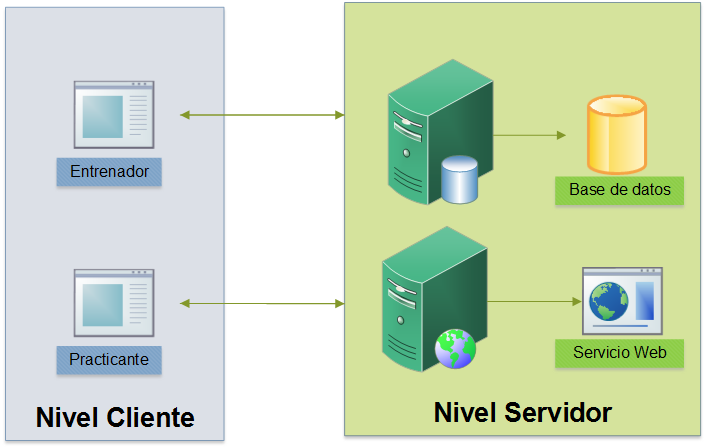
\includegraphics[scale=0.5]{./Figuras/Arquitectura/Arquitectura2Niveles}
	\end{center}
	\caption{Arquitectura de 2 Niveles}
	\label{fig:Arquitectura2Niveles}
\end{figure}

Se propone separar cada nivel aplicando el estilo por capas en la arquitectura cliente-servidor-cliente pues su objetivo principal es la separación de la lógica de negocio de la lógica de presentación.\\

\begin{itemize}
	\item \textbf{Capa de presentación.} Presenta el sistema al usuario, le comunica la información y captura la información del usuario en un mínimo de proceso. Esta capa se comunica únicamente con la capa de negocio.
	\item \textbf{Capa de negocio.} En esta capa se reciben las peticiones del usuario y se envían las respuestas tras el proceso. Se denomina capa de negocio (e incluso de lógica del negocio) porque es aquí donde se establecen todas las reglas de negocio que deben cumplirse. Esta capa se comunica con la capa de presentación, para recibir las solicitudes y presentar los resultados, y con la capa de datos, para solicitar al gestor de base de datos almacenar o recuperar datos de él.
	\item \textbf{Capa de datos.} Es la capa encargada de acceder a los datos. En esta capa se reciben solicitudes de almacenamiento o recuperación de información desde la capa de negocio.
	\item \textbf{Capa de datos compartidos.} En esta capa se mapean las entidades de la base de datos.
\end{itemize}

\begin{figure}[H]
	\begin{center}
		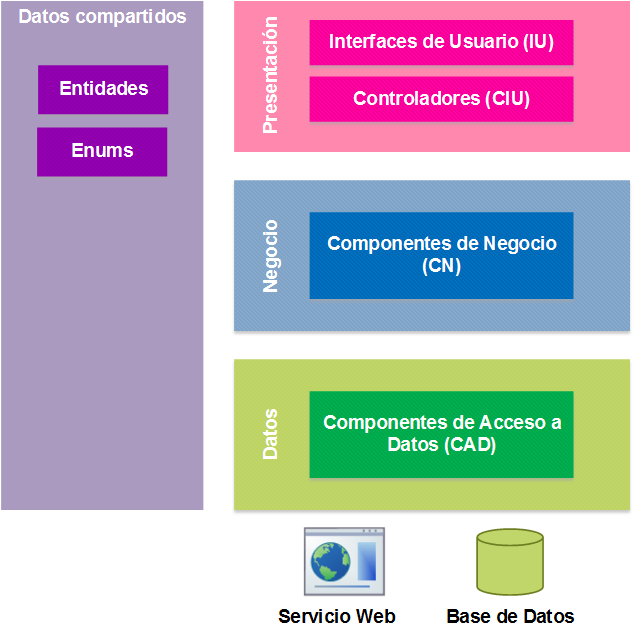
\includegraphics[scale=0.5]{./Figuras/Arquitectura/Arquitectura_enCapas}
	\end{center}
	\caption{Arquitectura en capas}
	\label{fig:Arquitectura_enCapas}
\end{figure}

Una arquitectura tiene muchas vistas posibles. Documentar todas las vistas potencialmente útiles representa en elevando consumo en tiempo y costo.\\

El modelo de 4+1 \cite{Kruchten} vistas fue desarrollado por Philippe Kruchten, el cual encaja con el estándar \textit{IEEE 1471-2000 Recommended Practice for Architecture Description of Software-Intensive Systems} \cite{IEEE1471} que se utiliza para describir la arquitectura de un sistema de software intensivo basado en el uso de múltiples puntos de vista. El modelo 4+1 describe la arquitectura del software usando cinco vistas concurrentes. Tal como se muestra en la Figura \ref{fig:Modelo} \nameref{fig:Modelo}, donde cada vista se refiere a un conjunto de intereses de diferentes stakeholders de sistema.

\begin{figure}[H]
	\begin{center}
		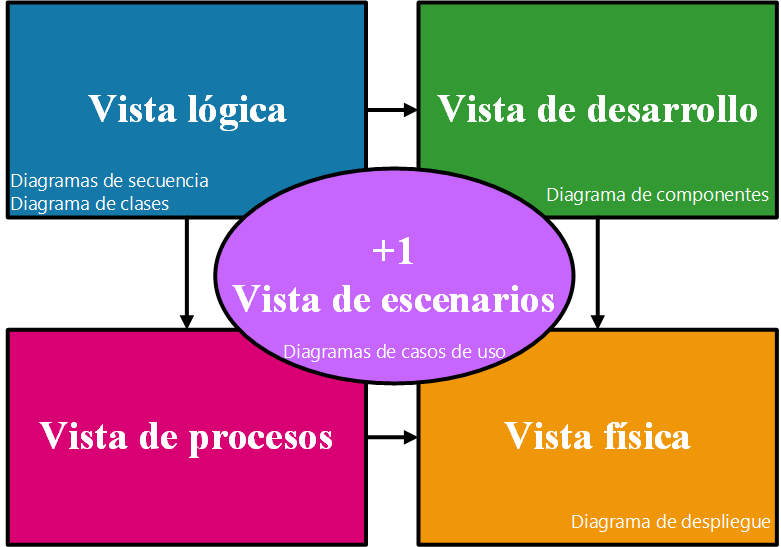
\includegraphics[scale=0.5]{./Figuras/Arquitectura/4+1Kruchten}
	\end{center}
	\caption{Modelo 4+1 de Kruchten}
	\label{fig:Modelo}
\end{figure}

\begin{itemize}
	\item La vista lógica describe el modelo de objetos del diseño cuando se usa un método de diseño orientado a objetos. 
	\item La vista de desarrollo describe la organización estática del software en su ambiente de desarrollo.
	\item La vista de procesos describe los aspectos de concurrencia y sincronización del diseño.
	\item La vista física describe el mapeo del software en el hardware y refleja los aspectos de distribución.
\end{itemize}

La descripción de las decisiones arquitecturales se pueden organizar en estas cuatro vistas y luego ilustrarlas con un conjunto reducido de casos de uso o escenarios, los cuales constituyen la quinta vista. La arquitectura evoluciona parcialmente a partir de esta vista de escenarios.\\

En el presente trabajo se expone una vista adicional al modelo 4+1, la vista de datos, en la cual se describe el esquema de la base de datos.\\

Cada vista se describe en un ``diagrama" que usa su notación particular.\\

\textbf{{\large{Vista lógica}}}\\

La vista lógica se apoya principalmente de los requisitos funcionales, es decir, lo que el sistema debe brindar en términos de servicios a sus usuarios. El sistema se descompone en un conjunto de abstracciones, tomadas en su mayoría del problema principal en forma de objetos o clases. Esta descomposición no solo sirve para el análisis funcional, también sirve para identificar mecanismos comunes y elementos de diseño a lo largo de varias partes del sistema.\\

\textbf{{\large{Vista de procesos}}}\\

La vista de procesos toma en cuenta algunos requisitos no funcionales tales como rendimiento y disponibilidad. Se enfoca en asuntos de concurrencia y distribución, integridad del sistema y de tolerancia a fallos. La vista de procesos también especifica en cuál hilo de control se ejecuta efectivamente una operación de una clase identificada en la vista lógica.\\

La arquitectura de procesos se describe en varios niveles de abstracción, donde cada nivel se refiere a distintos intereses. El nivel más alto de la arquitectura de procesos puede verse como un conjunto de redes lógicas de programas comunicantes (llamados "procesos") ejecutándose en forma independiente y/o distribuidos a lo largo de un conjunto de recursos de hardware.\\

Debido a que el presente Trabajo Terminal no contempla tácticas arquitecturales para atributos de calidad (disponibilidad, escalabilidad, etc) y a que la comunicación entre procesos se establecerá en el Trabajo Terminal 2, se omite la vista de procesos.\\

\textbf{{\large{Vista de desarrollo}}}\\

La vista de desarrollo se centra en la organización real de los módulos de software en el ambiente de desarrollo del software. El software se empaqueta en partes pequeñas – bibliotecas de programas o subsistemas – que pueden ser desarrollados por uno o un grupo pequeño de desarrolladores. Los subsistemas se organizan en una jerarquía de capas, cada una de las cuales brinda una interfaz estrecha y bien definida hacia las capas superiores.\\

\textbf{{\large{Vista física}}}\\

La vista física se enfoca en el mapeo de diferentes elementos identificados en las vistas lógica, de procesos y de desarrollo, en varios nodos.
El mapeo del software en nodos por lo tanto debe ser muy flexible y tener un impacto mínimo en el código.\\

\textbf{{\large{Vista de escenarios}}}\\

La vista de escenarios se encarga de mostrar las descripciones de las actividades que se deberán realizar para llevar a cabo procesos o tareas específicas del sistema, describiendo paso a paso la secuencia de interacciones entre los actores que participan en cada tarea.
Para cada escenario, se describen las correspondientes secuencias de interacciones entre objetos y procesos.

\clearpage


\section{Vista de escenarios}
La siguiente Figura \ref{fig:CU_General} \nameref{fig:CU_General} muestra  el diagrama de los casos de uso de la herramienta, contemplando a dos actores finales: Entrenador y Practicante.\\

\begin{figure}[H]
	\begin{center}
		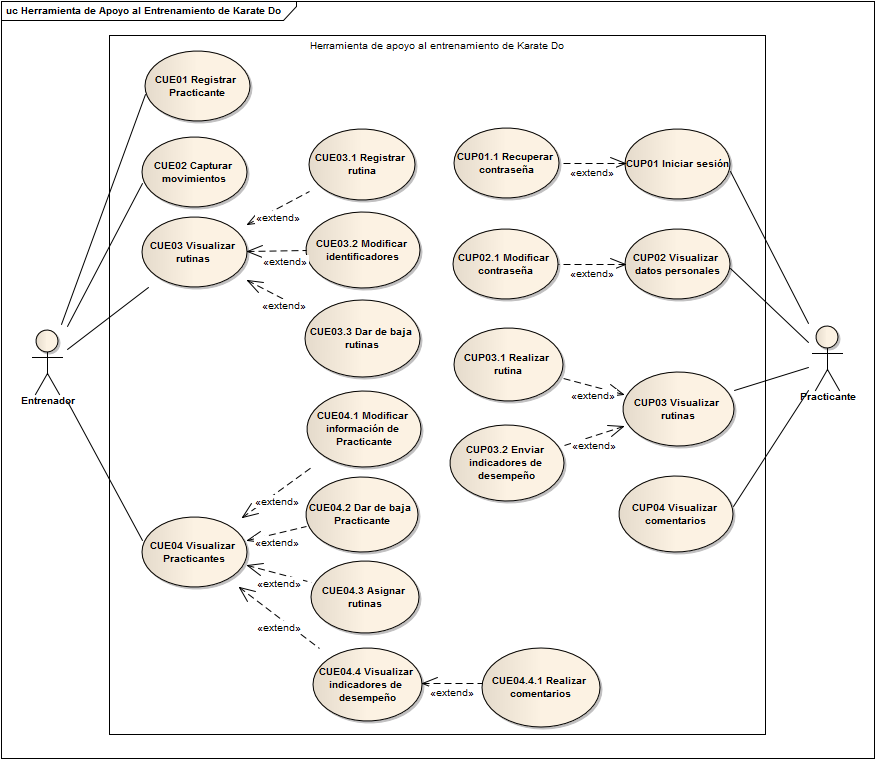
\includegraphics[scale=0.5]{./Figuras/Casos/CUGeneral}
	\end{center}
	\caption{Casos de uso Herramienta de apoyo al entrenamiento de Karate-Do}
	\label{fig:CU_General}
\end{figure}

\clearpage
%------------------------------------------------------------------------------------
\subsection{Casos de uso aplicación Entrenador}
La Figura \ref{fig:CU_Entrenador} \nameref{fig:CU_Entrenador} que se presenta a continuación, muestra el diagrama de los casos de uso correspondientes al actor Entrenador, además seguido de este se muestran las descripciones y trayectorias de cada uno de ellos.

\begin{figure}[H]
	\begin{center}
		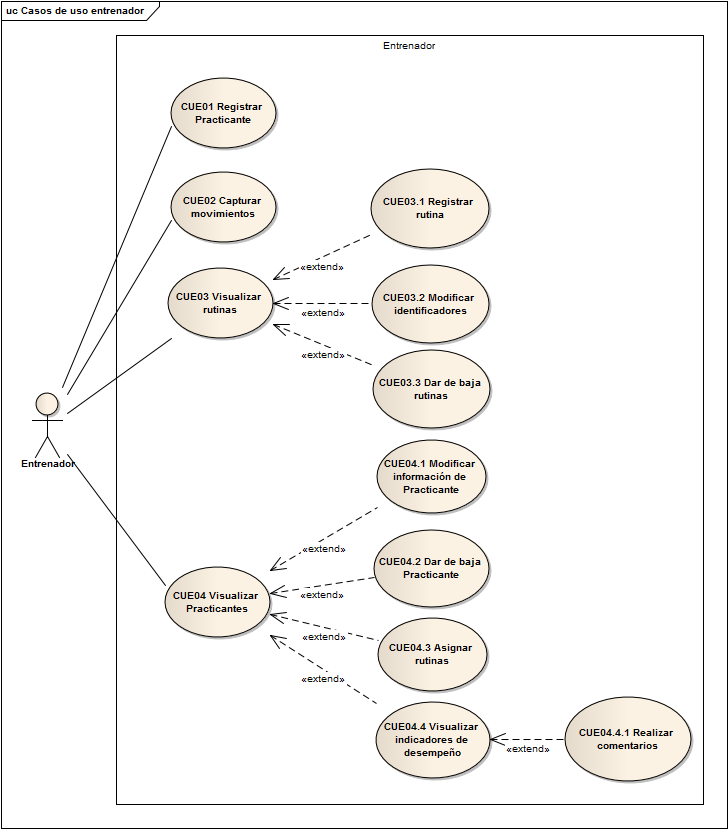
\includegraphics[scale=0.6]{./Figuras/Casos/Casos_de_uso_entrenador}
	\end{center}
	\caption{Casos de uso - Entrenador}
	\label{fig:CU_Entrenador}
\end{figure}

\subsubsection{CUE01 Registrar Practicante}
\label{cu:CUE01}
%--------------------------------------------------------------------------------------------------------
\textbf{\textcolor[rgb]{0, 0, 0.545098}{Resumen}} \\

Este caso de uso brinda al Entrenador la posibilidad de generar el registro de un Practicante, facilitando al Entrenador contar con un control de los Practicantes registrados en la herramienta así como de los datos relevantes de cada uno de ellos, de los cuales realiza el seguimiento de su desempeño.\\

\textbf{\textcolor[rgb]{0, 0, 0.545098}{Descripción}} \\

\begin{table}[H]
\centering
\begin{tabular}{| l | p{12 cm} |}
\hline
\rowcolor[rgb]{0.529412, 0.807843, 0.980392} {\textbf{Caso de uso:}} & \hspace{7em}{\textbf{CUE01 Registrar Practicante}}\\
\hline
\textbf{Actor:} &  \nameref{act:Entrenador}. \\
\hline
\textbf{Objetivo:} & Permitir al Entrenador registrar un nuevo Practicante.\\
\hline
\textbf{Entradas:} & Para llevar a cabo el registro de un nuevo Practicante, el Entrenador deberá hacer uso de la pantalla \nameref{pant:IUE01} y deberá capturar la siguiente información:
		\begin{compactitem} 
			\setlength\itemsep{-0.25em}
			\item Nombre(s)del usuario. Se escriben desde el teclado.
			\item Apellido(s). Se escriben desde el teclado.
			\item Edad. Se escribe desde el teclado.
			\item Domicilio. Se escribe desde el teclado.
			\item Teléfono. Se escribe desde el teclado.
			\item Correo electrónico. Se escribe desde el teclado.
			\item Avatar del Practicante. Se selecciona con el mouse.
			\item Peso. Se escribe desde el teclado.
			\item Estatura. Se escribe desde el teclado.
			\item Grupo sanguíneo. Se selecciona con el mouse.
			\item Grado de cinta. Se selecciona con el mouse.
			\item Nombre de usuario. Se escribe desde el teclado.
		\end{compactitem} \\
\hline
\textbf{Salidas:} & \vspace{-2mm}	%Para quitar el espacio en blanco de la fila
					\begin{compactitem}
						\setlength\itemsep{-0.25em}
						\item Se muestra en la pantalla \nameref{pant:IUE01}, el mensaje \nameref{msj:MSG01}, cuando se registre un Practicante de manera exitosa.
						\item Se envía al correo electrónico registrado el mensaje de tipo correo \nameref{msj:MSG08}, enviando la información de usuario y contraseña correspondiente.
					\end{compactitem}\\
\hline
\textbf{Precondiciones:} & \vspace{-2mm}	%Para quitar el espacio en blanco de la fila
							\begin{compactitem}
								\setlength\itemsep{-0.25em}
								\item El Practicante no debe estar registrado previamente en la herramienta.
							\end{compactitem}\\
\hline
\textbf{Postcondiciones:} & \vspace{-2mm}	%Para quitar el espacio en blanco de la fila
							\begin{compactitem}
								%\setlength\itemsep{-0.25em}
								\item Se registrará en la herramienta un nuevo Practicante.
								\item Se actualizará el catálogo: \textit{Practicantes}
							\end{compactitem}\\
\hline
\end{tabular}
\end{table} 

\begin{table}[H]
\centering
\begin{tabular}{| c | p{12 cm} |}
\hline
\textbf{Reglas de negocio:} & \vspace{-2mm}	%Para quitar el espacio en blanco de la fila
							\begin{compactitem}
								%\setlength\itemsep{-0.25em}
								\item \nameref{rn:RNR01}.
								\item \nameref{rn:RNR02}.
								\item \nameref{rn:RNR03}.
								\item \nameref{rn:RNR04}.
								\item \nameref{rn:RNR05}.
								\item \nameref{rn:RNR06}.
								\item \nameref{rn:RNR07}.
								\item \nameref{rn:RNR08}.
								\item \nameref{rn:RNR10}.
								\item \nameref{rn:RNR11}.
								\item \nameref{rn:RNR13}.
							\end{compactitem}\\		
\hline

\textbf{Errores:} & \vspace{-2mm}	%Para quitar el espacio en blanco de la fila
					\begin{compactitem}
						\setlength\itemsep{-0.25em}
						\item Se muestra en la pantalla \nameref{pant:IUE01} el mensaje de error \nameref{msj:MSG12} cuando el Entrenador no haya ingresado datos a los campos obligatorios.
						\item Se muestra en pantalla el mensaje de error \nameref{msj:MSG13} cuando el Entrenador haya ingresado datos con un formato incorrecto en algún campo.
						\item Se muestra en pantalla el mensaje de error \nameref{msj:MSG11} cuando el Entrenador intente registrar a un Practicante que ya se encuentre registrado en la herramienta.
					\end{compactitem}\\
\hline
\textbf{Tipo:} & Primario.\\
\hline	
\end{tabular}
\caption{Resumen de atributos de CUE01 Registrar Practicante}
\label{tab:CUE01}
\end{table} 

%--------------------------------------------------------------------------------------------------------
\textbf{\textcolor[rgb]{0, 0, 0.545098}{Trayectorias del caso de uso}} \\
%\textbf{Trayectorias del caso de uso} \\

\textbf{\large{Trayectoria principal}}

\begin{enumerate}
	\item 
\includegraphics[width=15pt, height=10pt]{./Figuras/iconosCU/usuario.png} Solicita registrar un nuevo \textit{Practicante} seleccionando la opción \textit{Registrar practicante} del menú \nameref{menu:ME02}.
	\item 
\includegraphics[width=15pt]{./Figuras/iconosCU/herramienta.png} Solicita al \textit{Entrenador} ingresar la información requerida para registrar un nuevo \textit{Practicante} mediante el uso de la pantalla \nameref{pant:IUE01}.
	\item 
\includegraphics[width=15pt, height=10pt]{./Figuras/iconosCU/usuario.png} Ingresa los datos del \textit{Practicante} a registrar, según la información especificada en la regla de negocio \nameref{rn:RNR02}.
	\item \includegraphics[width=15pt]{./Figuras/iconosCU/herramienta.png} Verifica que se hayan ingresado los valores en los campos obligatorios según lo especificado en la regla de negocio \nameref{rn:RNR01} y \nameref{rn:RNR03}. \textbf{[Trayectoria A]} 
	\item \includegraphics[width=15pt]{./Figuras/iconosCU/herramienta.png} Verifica que los valores en los campos cumplan con el formato correcto según lo especificado en las reglas de negocio \nameref{rn:RNR04}, \nameref{rn:RNR05}, \nameref{rn:RNR07} y \nameref{rn:RNR10}. \textbf{[Trayectoria B]}
	\item \includegraphics[width=15pt, height=10pt]{./Figuras/iconosCU/usuario.png} Solicita registrar al \textit{Practicante} seleccionando la opción \textit{Guardar}. \textbf{[Trayectoria C]}
	\item \includegraphics[width=15pt]{./Figuras/iconosCU/herramienta.png} Verifica que el nombre de usuario del \textit{Practicante} no se encuentre registrado en la herramienta, según lo especificado en la regla de negocio \nameref{rn:RNR06}.  \textbf{[Trayectoria D]}
	\item \includegraphics[width=15pt]{./Figuras/iconosCU/herramienta.png} Verifica que el \textit{Practicante} no se encuentre registrado en la herramienta, según lo especificado en la regla de negocio \nameref{rn:RNR13}. \textbf{[Trayectoria E]}
	\item \includegraphics[width=15pt]{./Figuras/iconosCU/herramienta.png} Genera una contraseña de manera aleatoria según lo especificado en la \nameref{rn:RNR08}.
	\item \includegraphics[width=15pt]{./Figuras/iconosCU/herramienta.png} Registra los datos del \textit{Practicante}.
	\item \includegraphics[width=15pt]{./Figuras/iconosCU/herramienta.png} Se envía por medio del mensaje de tipo correo \nameref{msj:MSG08} el nombre de usuario y la contraseña del Practicante recién registrado, según lo especificado en la \nameref{rn:RNR11}.
	\item \includegraphics[width=15pt]{./Figuras/iconosCU/herramienta.png} Muestra el mensaje de notificación \nameref{msj:MSG01}.
	\item \includegraphics[width=15pt]{./Figuras/iconosCU/herramienta.png} Regresa al menú \nameref{menu:ME02}.
\end{enumerate}
	
- - - - \textit{Fin del caso de uso.} \\

%.....................................................

\textbf{\large{Trayectoria alternativa A:}}\\
\textbf{Condición: } El \textit{Entrenador} no ingresó los valores correspondientes  en los campos marcados como obligatorios.

\begin{enumerate}
	\item \includegraphics[width=15pt]{./Figuras/iconosCU/herramienta.png} Muestra en la pantalla \nameref{pant:IUE01}, el mensaje de error \nameref{msj:MSG12}.
	\item \includegraphics[width=15pt]{./Figuras/iconosCU/herramienta.png} Continúa en el paso 3 de la trayectoria principal.
\end{enumerate}

- - - - \textit{Fin de trayectoria.} \\

%.....................................................
\textbf{\large{Trayectoria alternativa B:}}\\
\textbf{Condición: } El \textit{Entrenador} ingresó valores con un formato incorrecto.

\begin{enumerate}
	\item \includegraphics[width=15pt]{./Figuras/iconosCU/herramienta.png} Muestra en 
	pantalla el mensaje de error \nameref{msj:MSG13}.
	\item \includegraphics[width=15pt]{./Figuras/iconosCU/herramienta.png} Continúa en el paso 3 de la trayectoria principal.
\end{enumerate}

- - - - \textit{Fin de trayectoria.} \\

\textbf{\large{Trayectoria alternativa C:}}\\
\textbf{Condición: } El \textit{Entrenador} desea cancelar la operación.

\begin{enumerate}
	\item \includegraphics[width=15pt, height=25pt]{./Figuras/iconosCU/usuario.png} Solicita cancelar la operación seleccionando la opción \textit{Cancelar}.
	\item \includegraphics[width=15pt]{./Figuras/iconosCU/herramienta.png} Cancela la operación y regresa al menú \nameref{menu:ME02}.
	\item Fin del caso de uso.
\end{enumerate}

- - - - \textit{Fin de trayectoria.} \\

%.....................................................


%.....................................................
\textbf{\large{Trayectoria alternativa D:}}\\
\textbf{Condición: } El \textit{Entrenador} ingresa un nombre de usuario que se encuentra previamente registrado.

\begin{enumerate}
	\item \includegraphics[width=15pt]{./Figuras/iconosCU/herramienta.png} Muestra en pantalla el mensaje de error \nameref{msj:MSG11}.
	\item \includegraphics[width=15pt]{./Figuras/iconosCU/herramienta.png} Continúa en el paso 3 de la trayectoria principal.
\end{enumerate}

- - - - \textit{Fin de trayectoria.} \\

%.....................................................
\textbf{\large{Trayectoria alternativa E:}}\\
\textbf{Condición: } El \textit{Entrenador} desea registrar a un \textit{Practicante} que se encuentra previamente registrado.

\begin{enumerate}
	\item \includegraphics[width=15pt]{./Figuras/iconosCU/herramienta.png} Muestra en pantalla el mensaje de error \nameref{msj:MSG11}.
	\item \includegraphics[width=15pt]{./Figuras/iconosCU/herramienta.png} Continúa en el paso 3 de la trayectoria principal.
\end{enumerate}

- - - - \textit{Fin de trayectoria.} \\
%\newpage
\clearpage
\subsubsection{CUE02 Capturar movimientos}
\label{cu:CUE02}

\textbf{\textcolor[rgb]{0, 0, 0.545098}{Resumen}} \\

Este caso de uso brinda al Entrenador la posibilidad de capturar un movimiento de técnica de los disponibles en el catálogo de movimientos, para su posterior uso al crear rutinas.\\

\textbf{\textcolor[rgb]{0, 0, 0.545098}{Descripción}}

\begin{table}[H]
\centering
\begin{tabular}{| l | p{12 cm} |}
\hline
\rowcolor[rgb]{0.529412, 0.807843, 0.980392} {\textbf{Caso de uso:}} & \hspace{7em}{\textbf{CUE02 Capturar movimientos}}\\
\hline
\textbf{Actor:} &  \nameref{act:Entrenador}. \\
\hline
\textbf{Objetivo:} & Permitir al Entrenador capturar movimientos y guardarlos en la herramienta.\\
\hline
\textbf{Entradas:} & Para llevar a cabo el registro del movimiento capturado, el Entrenador debe hacer uso de la pantalla \nameref{pant:IUE02} donde el Entrenador debe capturar lo siguiente:
		\begin{compactitem} 
			\setlength\itemsep{-0.25em}
			\item Movimiento. Se obtiene mediante el sensor Kinect.
		\end{compactitem} \\
\hline
\textbf{Salidas:} & \vspace{-2mm}	%Para quitar el espacio en blanco de la fila
					\begin{compactitem}
						\setlength\itemsep{-0.25em}
						\item Se muestra en la pantalla \nameref{pant:IUE02} el mensaje de notificación \nameref{msj:MSG01},  cuando se registre el movimiento de manera exitosa.
					\end{compactitem}\\
\hline
\textbf{Precondiciones:} & 	\vspace{-2mm}	%Para quitar el espacio en blanco de la fila
							\begin{compactitem}
								\setlength\itemsep{-0.25em}
								\item Ninguna.
							\end{compactitem}\\
\hline
\textbf{Postcondiciones:} & \vspace{-2mm}	%Para quitar el espacio en blanco de la fila
							\begin{compactitem}
								\setlength\itemsep{-0.25em}
								\item Se registra en la herramienta un movimiento de técnica.
								\item Se actualizará la información del catálogo de \textit{movimientos de técnica}.
							\end{compactitem}\\
							
\hline
\textbf{Reglas de negocio:} & \vspace{-2mm}	%Para quitar el espacio en blanco de la fila
							\begin{compactitem}
								\setlength\itemsep{-0.25em}
								\item \nameref{rn:RNR34}
								\item \nameref{rn:RNR35}
								\item \nameref{rn:RNR36}
								\item \nameref{rn:RNR37}
								\item \nameref{rn:RNR38}
							\end{compactitem}\\							
\hline
\textbf{Errores:} &	\vspace{-2mm}	%Para quitar el espacio en blanco de la fila
					\begin{compactitem}
						\setlength\itemsep{-0.25em}
						\item Se muestra en la pantalla \nameref{pant:IUE02} el mensaje de error \nameref{msj:MSG25} cuando no se pueda guardar el movimiento en la base de datos.
					\end{compactitem}\\
\hline
\textbf{Tipo:} & Primario.\\
\hline	
\end{tabular}
\caption{Resumen de atributos de CUE02 Capturar movimientos}
\label{tab:CUE02}
\end{table} 
\clearpage

%--------------------------------------------------------------------------------------------------------
\textbf{\textcolor[rgb]{0, 0, 0.545098}{Trayectorias del caso de uso}} \\
%\textbf{Trayectorias del caso de uso} \\

\textbf{\large{Trayectoria principal}}

\begin{enumerate}
	\item \includegraphics[width=15pt, height=10pt]{./Figuras/iconosCU/usuario.png} Solicita capturar un movimiento seleccionando la opción \textit{Capturar} del menú principal \nameref{menu:ME01}.	
	\item \includegraphics[width=15pt]{./Figuras/iconosCU/herramienta.png} Muestra el menú de la pantalla \nameref{pant:IUE02}.
	\item \includegraphics[width=15pt, height=10pt]{./Figuras/iconosCU/usuario.png} Selecciona el movimiento a capturar del catálogo disponible mediante el gesto \textit{Seleccionar}.
	\item \includegraphics[width=15pt]{./Figuras/iconosCU/herramienta.png} Muestra la pantalla de captura \nameref{pant:IUE02}.
	\item \includegraphics[width=15pt, height=10pt]{./Figuras/iconosCU/usuario.png} Realiza el saludo de Karate Do.
	\item \includegraphics[width=15pt, height=10pt]{./Figuras/iconosCU/usuario.png} Se coloca en posición de alerta.
	\item \includegraphics[width=15pt, height=10pt]{./Figuras/iconosCU/usuario.png} Realiza el movimiento seleccionado según lo especificado en la regla de negocio \nameref{rn:RNR34} con ayuda del modelo que especifica la regla de negocio \nameref{rn:RNR35}. \textbf{[Trayectoria A]}
	\item \includegraphics[width=15pt]{./Figuras/iconosCU/herramienta.png} Comienza la captura del movimiento por medio del sensor Kinect según lo especificado en la regla de negocio \nameref{rn:RNR36}.
	\item \includegraphics[width=15pt, height=10pt]{./Figuras/iconosCU/usuario.png} Finaliza la captura del movimiento según lo especificado en la regla de negocio \nameref{rn:RNR37}. \textbf{[Trayectoria B]}
	\item \includegraphics[width=15pt]{./Figuras/iconosCU/herramienta.png} Captura el movimiento en el archivo según lo especificado en la regla de negocio \nameref{rn:RNR38}
	\item \includegraphics[width=15pt]{./Figuras/iconosCU/herramienta.png} Guarda el movimiento en la base de datos. \textbf{[Trayectoria C]}
	\item \includegraphics[width=15pt]{./Figuras/iconosCU/herramienta.png} Muestra el mensaje \nameref{msj:MSG01}.
\end{enumerate}
	
- - - - \textit{Fin del caso de uso.} \\


%.....................................................
\textbf{\large{Trayectoria alternativa A:}}\\
\textbf{Condición: } El \textit{Practicante} desea regresar a la pantalla anterior sin realizar la captura del movimiento.

\begin{enumerate}
	\item \includegraphics[width=15pt, height=10pt]{./Figuras/iconosCU/usuario.png} Solicita cancelar la operación y regresar a la pantalla anterior por medio del gesto \textit{Regresar}.
	\item \includegraphics[width=15pt]{./Figuras/iconosCU/herramienta.png} Regresa al menú de la pantalla \nameref{pant:IUE02}.
	\item Continua en el paso 3 de la trayectoria principal.
\end{enumerate}

- - - - \textit{Fin de trayectoria.} \\

%.....................................................
\textbf{\large{Trayectoria alternativa B:}}\\
\textbf{Condición: } El \textit{Entrenador} desea repetir el movimiento capturado.

\begin{enumerate}
	\item \includegraphics[width=15pt, height=10pt]{./Figuras/iconosCU/usuario.png} Solicita volver a capturar el movimiento colocándose en posición de alerta.
	\item \includegraphics[width=15pt]{./Figuras/iconosCU/herramienta.png} Continúa en el paso 6 de la trayectoria principal.
\end{enumerate}

- - - - \textit{Fin de trayectoria.} \\

%.....................................................
\textbf{\large{Trayectoria alternativa C:}}\\
\textbf{Condición: } La conexión ha fallado al guardar el movimiento capturado en la base de datos.

\begin{enumerate}
	\item \includegraphics[width=15pt]{./Figuras/iconosCU/herramienta.png} Muestra en la pantalla \nameref{pant:IUE02} el mensaje de error \nameref{msj:MSG25} cuando no se pueda guardar el movimiento en la base de datos.
	\item Continua en el paso 3 de la trayectoria principal.
\end{enumerate}

- - - - \textit{Fin de trayectoria.} \\

%\newpage
\clearpage
\subsubsection{CUE03 Visualizar rutinas}
\label{cu:CUE03}

\textbf{\textcolor[rgb]{0, 0, 0.545098}{Resumen}} \\

Este caso de uso brinda al Entrenador la posibilidad de visualizar la lista de ejercicios de calentamiento disponibles, la lista de movimientos de técnica capturados y la lista de las rutinas de entrenamiento registradas.\\

\textbf{\textcolor[rgb]{0, 0, 0.545098}{Descripción}}

\begin{table}[H]
\centering
\begin{tabular}{| l | p{12 cm} |}
\hline
\rowcolor[rgb]{0.529412, 0.807843, 0.980392} {\textbf{Caso de uso:}} & \hspace{7em}{\textbf{CUE03 Visualizar rutinas}}\\
\hline
\textbf{Actor:} &  \nameref{act:Entrenador}. \\
\hline
\textbf{Objetivo:} & Permitir al Entrenador visualizar las listas de movimientos y rutinas previamente registrados.\\
\hline
\textbf{Entradas:} & Para llevar a cabo los elementos, el Entrenador debe hacer uso de la pantalla \nameref{pant:IUE03}. \\
\hline
\textbf{Salidas:} & \vspace{-2mm}	%Para quitar el espacio en blanco de la fila
					\begin{compactitem}
						\setlength\itemsep{-0.25em}
						\item Ninguna.
					\end{compactitem}\\
\hline
\textbf{Precondiciones:} & 	\vspace{-2mm}	%Para quitar el espacio en blanco de la fila
							\begin{compactitem}
								\setlength\itemsep{-0.25em}
								\item Se requiere que existan elementos en al menos uno de los catálogos: ejercicios de calentamiento, movimientos de técnica y rutinas de entrenamiento.
							\end{compactitem}\\
\hline
\textbf{Postcondiciones:} & \vspace{-2mm}	%Para quitar el espacio en blanco de la fila
							\begin{compactitem}
								%\setlength\itemsep{-0.25em}
								\item Ninguna.
							\end{compactitem}\\
							
\hline
\textbf{Reglas de negocio:} & \vspace{-2mm}	%Para quitar el espacio en blanco de la fila
							\begin{compactitem}
								%\setlength\itemsep{-0.25em}
								\item Ninguna.
							\end{compactitem}\\							
\hline
\textbf{Errores:} &	\vspace{-2mm}	%Para quitar el espacio en blanco de la fila
					\begin{compactitem}
						\setlength\itemsep{-0.25em}
						\item  Se muestra en el menú principal \nameref{menu:ME01}, el mensaje de error \nameref{msj:MSG24}, cuando debido a un error de conexión no se muestren los elementos de forma correcta.
					\end{compactitem}\\
\hline
\textbf{Tipo:} & Primario.\\
\hline	
\end{tabular}
\caption{Resumen de atributos de CUE03 Visualizar rutinas}
\label{tab:CUE03}
\end{table} 

%--------------------------------------------------------------------------------------------------------
\textbf{\textcolor[rgb]{0, 0, 0.545098}{Trayectorias del caso de uso}} \\
%\textbf{Trayectorias del caso de uso} \\

\textbf{\large{Trayectoria principal}}

\begin{enumerate}
	\item \includegraphics[width=15pt, height=10pt]{./Figuras/iconosCU/usuario.png} Solicita visualizar los ejercicios de calentamiento, movimientos de técnica y rutinas de entrenamiento registrados en la herramienta seleccionando la opción \textit{Rutinas} del menú \nameref{menu:ME01}.
	\item \includegraphics[width=15pt]{./Figuras/iconosCU/herramienta.png} Busca la información en los catálogos de \textit{ejercicios de calentamiento, movimientos de técnica y rutinas de entrenamiento}. \textbf{[Trayectoria A]}
	\item \includegraphics[width=15pt]{./Figuras/iconosCU/herramienta.png} Muestra las listas rutinas, ejercicios de calentamiento y movimientos de técnica en la pantalla \nameref{pant:IUE03}. \textbf{[Trayectoria B]}
\end{enumerate}
	
- - - - \textit{Fin del caso de uso.} \\

%.....................................................
\textbf{\large{Trayectoria alternativa A:}}\\
\textbf{Condición: } Debido a un error de conexión, no se muestran los elementos de forma correcta.

\begin{enumerate}
	\item \includegraphics[width=15pt]{./Figuras/iconosCU/herramienta.png} Muestra en el menú principal \nameref{menu:ME01}, el mensaje de error \nameref{msj:MSG24}, indicando que la operación no puede continuar de forma correcta.
	\item Fin del caso de uso.
\end{enumerate}

- - - - \textit{Fin de trayectoria.} \\

%.....................................................
\textbf{\large{Trayectoria alternativa B:}}\\
\textbf{Condición: } El \textit{Entrenador} desea regresar a la pantalla anterior.

\begin{enumerate}
	\item \includegraphics[width=15pt, height=10pt]{./Figuras/iconosCU/usuario.png} Solicita regresar a la pantalla anterior seleccionando la opción \textit{Regresar}.
	\item \includegraphics[width=15pt]{./Figuras/iconosCU/herramienta.png} Muestra el menú principal \nameref{menu:ME01}.
	\item Fin del caso de uso.
\end{enumerate}

- - - - \textit{Fin de trayectoria.} \\

\textbf{\large{Extiende:}}

\begin{enumerate}
	\item \includegraphics[width=15pt]{./Figuras/iconosCU/herramienta.png} \nameref{cu:CUE03.1}
	\item \includegraphics[width=15pt]{./Figuras/iconosCU/herramienta.png} \nameref{cu:CUE03.2}
	\item \includegraphics[width=15pt]{./Figuras/iconosCU/herramienta.png} \nameref{cu:CUE03.3}
\end{enumerate}
%\newpage
\clearpage
\subsubsection{CUE03.1 Registrar rutina}
\label{cu:CUE03.1}

\textbf{\textcolor[rgb]{0, 0, 0.545098}{Resumen}} \\

Este caso de uso brinda al Entrenador la posibilidad de registrar una rutina de entrenamiento, compuesta por ejercicios de calentamiento y movimientos de técnica. El registro de las rutinas será realizado mediante la selección de los ejercicios y los movimientos registrados previamente, además del número de repeticiones para cada ejercicio y movimiento.\\

\textbf{\textcolor[rgb]{0, 0, 0.545098}{Descripción}} \\
%\textbf{Descripción} \\

\begin{table}[H]
\centering
\begin{tabular}{| c | p{12 cm} |}
\hline
\rowcolor[rgb]{0.529412, 0.807843, 0.980392} {\textbf{Caso de uso:}} & \hspace{7em}{\textbf{CUE03.1 Registrar rutina}}\\
\hline
\textbf{Actor:} &  \nameref{act:Entrenador}. \\
\hline
\textbf{Objetivo:} & Permitir al Entrenador registrar una nueva rutina de entrenamiento.\\
\hline
\textbf{Entradas:} & Para llevar a cabo el registro de una nueva rutina de entrenamiento, el Entrenador debe hacer uso de la pantalla \nameref{pant:IUE03.1} donde debe capturar la siguiente información:
	\begin{compactitem} 
			\setlength\itemsep{-0.25em}
			\item Nombre de la rutina de entrenamiento. Se escribe desde el teclado.
			\item Imagen alusiva a la rutina. Se selecciona con el mouse.
			\item Ejercicios de calentamiento. Se seleccionan con el mouse.
			\item Movimientos de técnica. Se seleccionan con el mouse.
			\item Repeticiones de cada ejercicio y movimiento. Se seleccionan con el mouse.
	\end{compactitem} \\
\hline
\textbf{Salidas:} & \vspace{-2mm}	%Para quitar el espacio en blanco de la fila
					\begin{compactitem}
						\setlength\itemsep{-0.25em}
						\item Se muestra en la pantalla \nameref{pant:IUE03.1} el mensaje de notificación \nameref{msj:MSG01} cuando se registre una rutina de manera exitosa.
						\item Se muestra en la pantalla \nameref{pant:IUE03} el mensaje de notificación \nameref{msj:MSG02}, cuando no existan elementos registrados en los catálogos correspondientes.
					\end{compactitem}\\
\hline
\textbf{Precondiciones:} & \vspace{-2mm}	%Para quitar el espacio en blanco de la fila
							\begin{compactitem}
								\setlength\itemsep{-0.25em}
								\item Se requiere que existan elementos en los catálogos: ejercicios de calentamiento y movimientos de técnica.
							\end{compactitem}\\
\hline
\textbf{Postcondiciones:} & \vspace{-2mm}	%Para quitar el espacio en blanco de la fila
							\begin{compactitem}
								%\setlength\itemsep{-0.25em}
								\item Se registrará en la herramienta una nueva rutina.
								\item Se actualizará la información del catálogo de rutinas.
							\end{compactitem}\\
\hline
\end{tabular}
\end{table} 

\begin{table}[H]
\centering
\begin{tabular}{| c | p{12 cm} |}
\hline
\textbf{Reglas de negocio:} & \vspace{-2mm}	%Para quitar el espacio en blanco de la fila
							\begin{compactitem}
								%\setlength\itemsep{-0.25em}
								\item \nameref{rn:RND02}.
								\item \nameref{rn:RNR01}.
								\item \nameref{rn:RNR14}.
								\item \nameref{rn:RNR15}.
								\item \nameref{rn:RNR16}.
								\item \nameref{rn:RNR17}.
							\end{compactitem}\\							
\hline

\textbf{Errores:} & \vspace{-2mm}	%Para quitar el espacio en blanco de la fila
					\begin{compactitem}
						\setlength\itemsep{-0.25em}
						\item Se muestra en la pantalla \nameref{pant:IUE03.1} el mensaje de error \nameref{msj:MSG12} cuando el Entrenador no haya ingresado datos a los campos obligatorios.
						\item Se muestra en pantalla el mensaje de error \nameref{msj:MSG13} cuando el Entrenador haya ingresado datos con formato incorrecto en un campo.
						\item Se muestra en pantalla el mensaje de error \nameref{msj:MSG16} cuando el Entrenador no haya seleccionado al menos 3 ejercicios de calentamiento o cuando haya seleccionado más de 5 ejercicios.
						\item Se muestra en pantalla el mensaje de error \nameref{msj:MSG16} cuando el Entrenador no haya seleccionado al menos 2 movimientos de técnica o cuando haya seleccionado más de 4 movimientos.
						\item Se muestra en pantalla el mensaje de error \nameref{msj:MSG20} cuando el Entrenador haya excedido el número de registros de rutinas permitidos.
					\end{compactitem}\\
\hline
\textbf{Tipo:} & Secundario, viene del \nameref{cu:CUE03}.\\
\hline	
\end{tabular}
\caption{Resumen de atributos de CUE03.1 Registrar rutina}
\label{tab:CUE031}
\end{table} 

%--------------------------------------------------------------------------------------------------------
\textbf{\textcolor[rgb]{0, 0, 0.545098}{Trayectorias del caso de uso}} \\
%\textbf{Trayectorias del caso de uso} \\

\textbf{\large{Trayectoria principal}}

\begin{enumerate}
	\item \includegraphics[width=15pt, height=10pt]{./Figuras/iconosCU/usuario.png} Solicita registrar una nueva rutina de entrenamiento seleccionando la opción \textit{Agregar rutina} de la pantalla \nameref{pant:IUE03}.
	\item \includegraphics[width=15pt]{./Figuras/iconosCU/herramienta.png} Busca la información de los catálogos ejercicios de calentamiento y movimientos de técnica. \textbf{[Trayectoria A]}
	\item \includegraphics[width=15pt]{./Figuras/iconosCU/herramienta.png} Solicita al \textit{Entrenador} ingresar la información requerida para registrar una nueva rutina mediante el uso de la pantalla \nameref{pant:IUE03.1}.
	\item \includegraphics[width=15pt, height=10pt]{./Figuras/iconosCU/usuario.png} Ingresa los identificadores de la rutina a registrar.
	\item \includegraphics[width=15pt, height=10pt]{./Figuras/iconosCU/usuario.png} Selecciona los ejercicios de calentamiento y movimientos de técnica que van a conformar la nueva rutina, según lo especificado en la \nameref{rn:RND02} dando clic sobre el control de cada uno.
	\item \includegraphics[width=15pt, height=10pt]{./Figuras/iconosCU/usuario.png} Selecciona el número de repeticiones por cada ejercicios de calentamiento y movimientos de técnica seleccionados.
	\item \includegraphics[width=15pt]{./Figuras/iconosCU/herramienta.png} Verifica que se hayan ingresado los valores en los campos obligatorios, según lo especificado en la regla de negocio \nameref{rn:RNR01} y \nameref{rn:RNR14}. \textbf{[Trayectoria B]}
	\item \includegraphics[width=15pt]{./Figuras/iconosCU/herramienta.png} Verifica que los valores ingresados cumplan con el formato correcto, según lo especificado en la regla de negocio \nameref{rn:RNR15}. \textbf{[Trayectoria C]} \textbf{[Trayectoria D]} \textbf{[Trayectoria E]} 
	\item \includegraphics[width=15pt, height=10pt]{./Figuras/iconosCU/usuario.png} Solicita guardar la información de la nueva rutina seleccionando la opción \textit{Guardar}. \textbf{[Trayectoria F]}
	\item \includegraphics[width=15pt]{./Figuras/iconosCU/herramienta.png} Verifica que no se haya alcanzado el número máximo de rutinas permitidas según lo especificado en la regla de negocio \nameref{rn:RNR17}. \textbf{[Trayectoria G]}
	\item \includegraphics[width=15pt]{./Figuras/iconosCU/herramienta.png} Registra los datos de la rutina de entrenamiento en el orden correcto según lo especificado en la regla de negocio \nameref{rn:RNR16}.
	\item \includegraphics[width=15pt]{./Figuras/iconosCU/herramienta.png} Muestra el mensaje de notificación \nameref{msj:MSG01}.
	\item \includegraphics[width=15pt]{./Figuras/iconosCU/herramienta.png} Regresa a la pantalla \nameref{pant:IUE03}.
\end{enumerate}
	
- - - - \textit{Fin del caso de uso.} \\

%.....................................................
\textbf{\large{Trayectoria alternativa A:}}\\
\textbf{Condición: } No se encontraron al menos dos movimientos de técnica capturados.

\begin{enumerate}
	\item \includegraphics[width=15pt]{./Figuras/iconosCU/herramienta.png} Muestra en la pantalla \nameref{pant:IUE03} el mensaje de notificación \nameref{msj:MSG02}, indicando que no hay datos en los catálogos necesarios y la operación no puede continuar.
	\item Fin del caso de uso.
\end{enumerate}

- - - - \textit{Fin de trayectoria.} \\

%.....................................................
\textbf{\large{Trayectoria alternativa B:}}\\
\textbf{Condición: } El \textit{Entrenador} no ingresó los valores correspondientes  en los campos marcados como obligatorios.

\begin{enumerate}
	\item \includegraphics[width=15pt]{./Figuras/iconosCU/herramienta.png} Muestra en la pantalla \nameref{pant:IUE03.1}, el mensaje de error \nameref{msj:MSG12}.
	\item \includegraphics[width=15pt]{./Figuras/iconosCU/herramienta.png} Continúa en el paso 4 de la trayectoria principal.
\end{enumerate}

- - - - \textit{Fin de trayectoria.} \\

%.....................................................
\textbf{\large{Trayectoria alternativa C:}}\\
\textbf{Condición: } El \textit{Entrenador} ingresó valores con un formato incorrecto.

\begin{enumerate}
	\item \includegraphics[width=15pt]{./Figuras/iconosCU/herramienta.png} Muestra en pantalla el mensaje de error \nameref{msj:MSG13}.
	\item \includegraphics[width=15pt]{./Figuras/iconosCU/herramienta.png} Continúa en el paso 5 de la trayectoria principal.
\end{enumerate}

- - - - \textit{Fin de trayectoria.} \\

%.....................................................
\textbf{\large{Trayectoria alternativa D:}}\\
\textbf{Condición: } El \textit{Entrenador} no seleccionó al menos 3 ejercicios de calentamiento y/o seleccionó más de 5 ejercicios.

\begin{enumerate}
	\item \includegraphics[width=15pt]{./Figuras/iconosCU/herramienta.png} Muestra en pantalla el mensaje de error \nameref{msj:MSG16}.
	\item \includegraphics[width=15pt]{./Figuras/iconosCU/herramienta.png} Continúa en el paso 5 de la trayectoria principal.
\end{enumerate}

- - - - \textit{Fin de trayectoria.} \\

%.....................................................
\textbf{\large{Trayectoria alternativa E:}}\\
\textbf{Condición: } El \textit{Entrenador} no seleccionó al menos 2 movimientos de técnica y/o seleccionó más de 4 movimientos.

\begin{enumerate}
	\item \includegraphics[width=15pt]{./Figuras/iconosCU/herramienta.png} Muestra en pantalla el mensaje de error \nameref{msj:MSG16}.
	\item \includegraphics[width=15pt]{./Figuras/iconosCU/herramienta.png} Continúa en el paso 5 de la trayectoria principal.
\end{enumerate}

- - - - \textit{Fin de trayectoria.} \\

%.....................................................
\textbf{\large{Trayectoria alternativa F:}}\\
\textbf{Condición: } El \textit{Entrenador} desea cancelar la operación.

\begin{enumerate}
	\item \includegraphics[width=15pt, height=10pt]{./Figuras/iconosCU/usuario.png} Solicita cancelar la operación seleccionando la opción \textit{Cancelar}.
	\item \includegraphics[width=15pt]{./Figuras/iconosCU/herramienta.png} Cancela la operación y regresa a la pantalla \nameref{pant:IUE03}.
	\item Fin del caso de uso.
\end{enumerate}

- - - - \textit{Fin de trayectoria.} \\

%.....................................................
\textbf{\large{Trayectoria alternativa G:}}\\
\textbf{Condición: } El \textit{Entrenador} intenta registrar más de 24 rutinas.

\begin{enumerate}
	\item \includegraphics[width=15pt]{./Figuras/iconosCU/herramienta.png} Muestra en pantalla el mensaje de error \nameref{msj:MSG20}.
	\item \includegraphics[width=15pt]{./Figuras/iconosCU/herramienta.png} Regresa a la pantalla \nameref{pant:IUE03}.
	\item Fin del caso de uso.
\end{enumerate}

- - - - \textit{Fin de trayectoria.} \\

%\newpage
\clearpage
\subsubsection{CUE03.2 Modificar identificadores}
\label{cu:CUE03.2}

\textbf{\textcolor[rgb]{0, 0, 0.545098}{Resumen}} \\

Este caso de uso brinda al Entrenador la posibilidad de modificar algún identificador (nombre o imagen alusiva) de algún de alguna rutina de entrenamiento.\\

\textbf{\textcolor[rgb]{0, 0, 0.545098}{Descripción}}

\begin{table}[H]
\centering
\begin{tabular}{| l | p{12 cm} |}
\hline
\rowcolor[rgb]{0.529412, 0.807843, 0.980392} {\textbf{Caso de uso:}} & \hspace{7em}{\textbf{CUE03.2 Modificar identificadores}}\\
\hline
\textbf{Actor:} &  \nameref{act:Entrenador}. \\
\hline
\textbf{Objetivo:} & Permitir al Entrenador modificar algún identificador.\\
\hline
\textbf{Entradas:} & Para llevar a cabo modificación de algún identificador, el Entrenador debe hacer uso de las pantalla \nameref{pant:IUE03.2} donde debe capturar la siguiente información:
		\begin{compactitem} 
			\setlength\itemsep{-0.25em}
			\item Nombre del identificador. Se escribe desde el teclado.
			\item Imagen alusiva a la rutina. Se selecciona con el mouse.
		\end{compactitem} \\
\hline
\textbf{Salidas:} & \vspace{-2mm}	%Para quitar el espacio en blanco de la fila
					\begin{compactitem}
						\setlength\itemsep{-0.25em}
						\item Se muestra en la pantalla \nameref{pant:IUE03.2} el mensaje de notificación \nameref{msj:MSG01}, cuando se modifique el identificador de manera exitosa.
					\end{compactitem}\\
\hline
\textbf{Precondiciones:} & 	\vspace{-2mm}	%Para quitar el espacio en blanco de la fila
							\begin{compactitem}
								\setlength\itemsep{-0.25em}
								\item Ninguna.
							\end{compactitem}\\
\hline
\textbf{Postcondiciones:} & \vspace{-2mm}	%Para quitar el espacio en blanco de la fila
							\begin{compactitem}
								%\setlength\itemsep{-0.25em}
								\item Se actualizará la información del catálogo de \textit{rutinas}.
							\end{compactitem}\\
							
\hline
\textbf{Reglas de negocio:} & \vspace{-2mm}	%Para quitar el espacio en blanco de la fila
							\begin{compactitem}
								%\setlength\itemsep{-0.25em}
								\item \nameref{rn:RNR01}.
								\item \nameref{rn:RNR14}.
								\item \nameref{rn:RNR15}.
							\end{compactitem}\\						
\hline
\textbf{Errores:} &	\vspace{-2mm}	%Para quitar el espacio en blanco de la fila
					\begin{compactitem}
						\setlength\itemsep{-0.25em}
							\item Se muestra en la pantalla \nameref{pant:IUE03.2} el mensaje de error \nameref{msj:MSG12} cuando el Entrenador no haya ingresado datos a los campos obligatorios.
							\item Se muestra en pantalla el mensaje de error \nameref{msj:MSG13} cuando el Entrenador haya ingresado datos con un formato incorrecto en algún campo.
						\end{compactitem}\\
\hline
\textbf{Tipo:} & Secundario, viene del \nameref{cu:CUE03}.\\
\hline	
\end{tabular}
\caption{Resumen de atributos de CUE03.2 Modificar identificadores}
\label{tab:CUE03.2}
\end{table} 

\clearpage
%--------------------------------------------------------------------------------------------------------
\textbf{\textcolor[rgb]{0, 0, 0.545098}{Trayectorias del caso de uso}} \\
%\textbf{Trayectorias del caso de uso} \\

\textbf{\large{Trayectoria principal}}

\begin{enumerate}
	\item \includegraphics[width=15pt, height=10pt]{./Figuras/iconosCU/usuario.png} Solicita modificar algún identificador de las rutinas enlistadas seleccionando el elemento deseado de la pantalla \nameref{pant:IUE03}.
	\item \includegraphics[width=15pt]{./Figuras/iconosCU/herramienta.png} Muestra el menú \nameref{menu:ME03}.
	\item \includegraphics[width=15pt, height=10pt]{./Figuras/iconosCU/usuario.png} Selecciona la opción \textit{Modificar}.
	\item \includegraphics[width=15pt]{./Figuras/iconosCU/herramienta.png} Solicita al \textit{Entrenador} ingresar la información requerida para modificar el/los identificador(es) nuevo(s) mediante el uso de la pantalla \nameref{pant:IUE03.2}.
	\item \includegraphics[width=15pt, height=10pt]{./Figuras/iconosCU/usuario.png} Ingresa el/los identificador(es) nuevo(s).
	\item \includegraphics[width=15pt]{./Figuras/iconosCU/herramienta.png} Verifica que se hayan ingresado los valores en los campos obligatorios, según lo especificado en la regla de negocio \nameref{rn:RNR01} y \nameref{rn:RNR14}. \textbf{[Trayectoria A]}
	\item \includegraphics[width=15pt]{./Figuras/iconosCU/herramienta.png} Verifica que los valores en los campos cumplan con el formato correcto según lo especificado en la regla de negocio \nameref{rn:RNR15}. \textbf{[Trayectoria B]}
	\item \includegraphics[width=15pt, height=10pt]{./Figuras/iconosCU/usuario.png} Solicita guardar los nuevos identificadores seleccionando la opción \textit{Guardar}. \textbf{[Trayectoria C]}
	\item \includegraphics[width=15pt]{./Figuras/iconosCU/herramienta.png} Registra el/los nuevo(s) identificador(es).
	\item \includegraphics[width=15pt]{./Figuras/iconosCU/herramienta.png} Muestra el mensaje de notificación \nameref{msj:MSG01}.
	\item \includegraphics[width=15pt]{./Figuras/iconosCU/herramienta.png} Regresa a la pantalla \nameref{pant:IUE03}.	
\end{enumerate}
	
- - - - \textit{Fin del caso de uso.} \\

%.....................................................
\textbf{\large{Trayectoria alternativa A:}}\\
\textbf{Condición: } El \textit{Entrenador} no ingresó los valores correspondientes en los campos marcados como obligatorios.

\begin{enumerate}
	\item \includegraphics[width=15pt]{./Figuras/iconosCU/herramienta.png} Muestra en la pantalla \nameref{pant:IUE03.2}, el mensaje de error \nameref{msj:MSG12}.
	\item \includegraphics[width=15pt]{./Figuras/iconosCU/herramienta.png} Continúa en el paso 4 de la trayectoria principal.
\end{enumerate}

- - - - \textit{Fin de trayectoria.} \\

%.....................................................
\textbf{\large{Trayectoria alternativa B:}}\\
\textbf{Condición: } El \textit{Entrenador} ingresó valores con un formato incorrecto.

\begin{enumerate}
	\item \includegraphics[width=15pt]{./Figuras/iconosCU/herramienta.png} Muestra en pantalla el mensaje de error \nameref{msj:MSG13}.
	\item \includegraphics[width=15pt]{./Figuras/iconosCU/herramienta.png} Continúa en el paso 4 de la trayectoria principal.
\end{enumerate}

- - - - \textit{Fin de trayectoria.} \\

%.....................................................
\textbf{\large{Trayectoria alternativa C:}}\\
\textbf{Condición: } El \textit{Entrenador} desea cancelar la operación.

\begin{enumerate}
	\item \includegraphics[width=15pt, height=10pt]{./Figuras/iconosCU/usuario.png} Solicita cancelar la operación seleccionando el botón \textit{Cancelar}.
	\item \includegraphics[width=15pt]{./Figuras/iconosCU/herramienta.png} Cancela la operación y regresa a la pantalla \nameref{pant:IUE03}.
	\item Fin del caso de uso.
\end{enumerate}


- - - - \textit{Fin de trayectoria.} \\
%\newpage
\clearpage
\subsubsection{CUE03.3 Dar de baja rutinas}
\label{cu:CUE03.3}

\textbf{\textcolor[rgb]{0, 0, 0.545098}{Resumen}} \\

Este caso de uso brinda al Entrenador la posibilidad de eliminar alguna de las rutinas de entrenamiento previamente registradas.\\

\textbf{\textcolor[rgb]{0, 0, 0.545098}{Descripción}}

\begin{table}[H]
\centering
\begin{tabular}{| l | p{12 cm} |}
\hline
\rowcolor[rgb]{0.529412, 0.807843, 0.980392} {\textbf{Caso de uso:}} & \hspace{7em}{\textbf{CUE03.3 Dar de baja rutinas}}\\
\hline
\textbf{Actor:} &  \nameref{act:Entrenador}. \\
\hline
\textbf{Objetivo:} & Permitir al Entrenador eliminar alguna rutina de entrenamiento.\\
\hline
\textbf{Entradas:} & Para realizar alguna eliminación, el Entrenador debe hacer uso del menú \nameref{menu:ME03} en la pantalla \nameref{pant:IUE03}. \\
\hline
\textbf{Salidas:} & \vspace{-2mm}	%Para quitar el espacio en blanco de la fila
					\begin{compactitem}
						\setlength\itemsep{-0.25em}
						\item Se muestra en la pantalla \nameref{pant:IUE03}, el mensaje de notificación \nameref{msj:MSG01}, cuando se realice una eliminación exitosa.
					\end{compactitem}\\
\hline
\textbf{Precondiciones:} & 	\vspace{-2mm}	%Para quitar el espacio en blanco de la fila
							\begin{compactitem}
								\setlength\itemsep{-0.25em}
								\item Deben existir elementos en los catálogos de \textit{rutinas}.
							\end{compactitem}\\
\hline
\textbf{Postcondiciones:} & \vspace{-2mm}	%Para quitar el espacio en blanco de la fila
							\begin{compactitem}
								%\setlength\itemsep{-0.25em}
								\item Se actualizará el catálogo de rutinas eliminando el elemento seleccionado.
							\end{compactitem}\\
							
\hline
\textbf{Reglas de negocio:} & \vspace{-2mm}	%Para quitar el espacio en blanco de la fila
							\begin{compactitem}
								%\setlength\itemsep{-0.25em}
								\item \nameref{rn:RNR24}.
							\end{compactitem}\\							
\hline
\textbf{Errores:} &	\vspace{-2mm}	%Para quitar el espacio en blanco de la fila
					\begin{compactitem}
						\setlength\itemsep{-0.25em}
						\item Se muestra en la pantalla \nameref{pant:IUE03} el mensaje de error \nameref{msj:MSG09}, cuando el Entrenador desee eliminar una rutina que se encuentre asignada a un Practicante.
					\end{compactitem}\\
\hline
\textbf{Tipo:} & Secundario, viene del \nameref{cu:CUE03}.\\
\hline	
\end{tabular}
\caption{Resumen de atributos de CUE03.3 Dar de baja rutinas}
\label{tab:CUE033}
\end{table} 

%--------------------------------------------------------------------------------------------------------
\textbf{\textcolor[rgb]{0, 0, 0.545098}{Trayectorias del caso de uso}} \\
%\textbf{Trayectorias del caso de uso} \\

\textbf{\large{Trayectoria principal}}

\begin{enumerate}
	\item \includegraphics[width=15pt, height=10pt]{./Figuras/iconosCU/usuario.png} Solicita eliminar alguno de los elementos enlistados seleccionando el elemento deseado de la pantalla \nameref{pant:IUE03}.
	\item \includegraphics[width=15pt]{./Figuras/iconosCU/herramienta.png} Muestra el menú \nameref{menu:ME03}.
	\item \includegraphics[width=15pt, height=10pt]{./Figuras/iconosCU/usuario.png} Selecciona la opción \textit{Eliminar}.
	\item \includegraphics[width=15pt]{./Figuras/iconosCU/herramienta.png} Muestra el mensaje de confirmación \nameref{msj:MSG04}.
	\item \includegraphics[width=15pt, height=10pt]{./Figuras/iconosCU/usuario.png} Selecciona la opción \textit{Aceptar}. \textbf{[Trayectoria A]} 
	\item \includegraphics[width=15pt]{./Figuras/iconosCU/herramienta.png} Verifica que el elemento seleccionado no se encuentre asignado a un \textit{Practicante}, según lo especificado en la regla de negocio \nameref{rn:RNR24}. \textbf{[Trayectoria B]}
	\item \includegraphics[width=15pt]{./Figuras/iconosCU/herramienta.png} Muestra el mensaje de notificación \nameref{msj:MSG01} y regresa a la pantalla \nameref{pant:IUE03}.
\end{enumerate}
	
- - - - \textit{Fin del caso de uso.} \\

%.....................................................
\textbf{\large{Trayectoria alternativa A:}}\\
\textbf{Condición: } El \textit{Entrenador} desea cancelar la operación.

\begin{enumerate}
	\item \includegraphics[width=15pt, height=10pt]{./Figuras/iconosCU/usuario.png} Solicita cancelar la operación seleccionando la opción \textit{Cancelar}.
	\item \includegraphics[width=15pt]{./Figuras/iconosCU/herramienta.png} Cancela la operación y regresa a la pantalla \nameref{pant:IUE03}.
	\item Fin del caso de uso.
\end{enumerate}

- - - - \textit{Fin de trayectoria.} \\

%.....................................................
\textbf{\large{Trayectoria alternativa B:}}\\
\textbf{Condición: } El \textit{Entrenador} desea eliminar una rutina que se encuentre asignada a un \textit{Practicante}.

\begin{enumerate}
	\item \includegraphics[width=15pt]{./Figuras/iconosCU/herramienta.png} Muestra el mensaje de error \nameref{msj:MSG09}, indicando que la rutina se encuentra asignada a un \textit{Practicante} y la operación no puede continuar.
	\item Fin del caso de uso.
\end{enumerate}
- - - - \textit{Fin de trayectoria.} \\

%\newpage
\clearpage
\subsubsection{CUE04 Visualizar Practicantes}
\label{cu:CUE04}

\textbf{\textcolor[rgb]{0, 0, 0.545098}{Resumen}} \\

Este caso de uso brinda la posibilidad de visualizar la lista de Practicantes registrados en la herramienta.\\

\textbf{\textcolor[rgb]{0, 0, 0.545098}{Descripción}} \\
%\textbf{Descripción} \\

\begin{table}[H]
\centering
\begin{tabular}{| c | p{12 cm} |}
\hline
\rowcolor[rgb]{0.529412, 0.807843, 0.980392} {\textbf{Caso de uso:}} & \hspace{7em}{\textbf{CUE04 Visualizar Practicantes}}\\
\hline
\textbf{Actor:} &  \nameref{act:Entrenador} \\
\hline
\textbf{Objetivo:} & Visualizar la lista de los Practicantes previamente registrados.\\
\hline
\textbf{Entradas:} & Para llevar a cabo la visualización de la lista de Practicantes, el Entrenador debe hacer uso de la pantalla \nameref{pant:IUE04}.\\
\hline
\textbf{Salidas:} & \vspace{-2mm}	%Para quitar el espacio en blanco de la fila
					\begin{compactitem}
						\setlength\itemsep{-0.25em}
						\item Ninguna.
					\end{compactitem}\\

\hline
\textbf{Precondiciones:} & \vspace{-2mm}	%Para quitar el espacio en blanco de la fila
							\begin{compactitem}
								\setlength\itemsep{-0.25em}
								\item Se requiere que existan elementos en el catálogo: \textit{Practicantes}.
							\end{compactitem}\\
\hline
\textbf{Postcondiciones:} & \vspace{-2mm}	%Para quitar el espacio en blanco de la fila
							\begin{compactitem}
								%\setlength\itemsep{-0.25em}
								\item Ninguna
							\end{compactitem}\\
\hline
\textbf{Reglas de negocio:} & \vspace{-2mm}	%Para quitar el espacio en blanco de la fila
							\begin{compactitem}
								%\setlength\itemsep{-0.25em}
								\item Ninguna.
							\end{compactitem}\\							
\hline
\textbf{Errores:} & \vspace{-2mm}	%Para quitar el espacio en blanco de la fila
					\begin{compactitem}
						\setlength\itemsep{-0.25em}
						\item  Se muestra en el menú principal \nameref{menu:ME02}, el mensaje de error \nameref{msj:MSG24}, cuando cuando debido a un error de conexión no se muestren los elementos de forma correcta.
					\end{compactitem}\\
\hline
\textbf{Tipo:} & Primario.\\
\hline	
\end{tabular}
\caption{Resumen de atributos de CUE04 Visualizar Practicantes}
\label{tab:CUE04}
\end{table} 

%--------------------------------------------------------------------------------------------------------
\textbf{\textcolor[rgb]{0, 0, 0.545098}{Trayectorias del caso de uso}} \\
%\textbf{Trayectorias del caso de uso} \\

\textbf{\large{Trayectoria principal}}

\begin{enumerate}
	\item \includegraphics[width=15pt, height=10pt]{./Figuras/iconosCU/usuario.png} Solicita visualizar la lista de Practicantes seleccionando la opción \textit{Lista de Practicantes} del menú \nameref{menu:ME02}. 
	\item \includegraphics[width=15pt]{./Figuras/iconosCU/herramienta.png} Busca la información del catálogo lista de Practicantes. \textbf{[Trayectoria A]}
	\item \includegraphics[width=15pt]{./Figuras/iconosCU/herramienta.png} Muestra la pantalla \nameref{pant:IUE04}. \textbf{[Trayectoria B]}
\end{enumerate}
	
- - - - \textit{Fin del caso de uso.} \\

%.....................................................
\textbf{\large{Trayectoria alternativa A:}}\\
\textbf{Condición: } Debido a un error de conexión, no se muestran los elementos de forma correcta.

\begin{enumerate}
	\item \includegraphics[width=15pt]{./Figuras/iconosCU/herramienta.png} Muestra en el menú \nameref{menu:ME02}, el mensaje de error \nameref{msj:MSG24}, indicando que la operación no puede continuar de forma correcta.
	\item Fin del caso de uso.
\end{enumerate}

- - - - \textit{Fin de trayectoria.} \\

%.....................................................
\textbf{\large{Trayectoria alternativa B:}}\\
\textbf{Condición: } El \textit{Entrenador} desea regresar a la pantalla anterior.

\begin{enumerate}
	\item \includegraphics[width=15pt, height=10pt]{./Figuras/iconosCU/usuario.png} Solicita regresar a la pantalla anterior presionando el botón \textit{Regresar}.
	\item \includegraphics[width=15pt]{./Figuras/iconosCU/herramienta.png} Muestra el menú \nameref{menu:ME02}.
	\item Fin del caso de uso.
\end{enumerate}

- - - - \textit{Fin de trayectoria.} \\

\textbf{\large{Extiende:}}

\begin{enumerate}
	\item \includegraphics[width=15pt]{./Figuras/iconosCU/herramienta.png} \nameref{cu:CUE04.1}
	\item \includegraphics[width=15pt]{./Figuras/iconosCU/herramienta.png} \nameref{cu:CUE04.2}
	\item \includegraphics[width=15pt]{./Figuras/iconosCU/herramienta.png} \nameref{cu:CUE04.3}
	\item \includegraphics[width=15pt]{./Figuras/iconosCU/herramienta.png} \nameref{cu:CUE04.4}
\end{enumerate}

%\newpage
\clearpage
\subsubsection{CUE04.1 Modificar información de Practicante}
\label{cu:CUE04.1}

\textbf{\textcolor[rgb]{0, 0, 0.545098}{Resumen}} \\

Este caso de uso brinda al Entrenador la posibilidad de modificar los datos personales de algún Practicante seleccionado.\\

\textbf{\textcolor[rgb]{0, 0, 0.545098}{Descripción}}

\begin{table}[H]
\centering
\begin{tabular}{| l | p{12 cm} |}
\hline
\rowcolor[rgb]{0.529412, 0.807843, 0.980392} {\textbf{Caso de uso:}} & \hspace{4em}{\textbf{CUE04.1 Modificar información de Practicante}}\\
\hline
\textbf{Actor:} &  \nameref{act:Entrenador}. \\
\hline
\textbf{Objetivo:} & Permitir al Entrenador modificar los datos de un Practicante.\\
\hline
\textbf{Entradas:} & Para llevar a cabo la modificación de alguno de los datos del Practicante, el Entrenador debe hacer uso de la pantalla \nameref{pant:IUE04.1} y debe capturar la siguiente información:
		\begin{compactitem} 
			\setlength\itemsep{-0.25em}
			\item Nombre(s)del usuario. Se escriben desde el teclado.
			\item Apellido(s). Se escriben desde el teclado.
			\item Edad. Se escribe desde el teclado.
			\item Domicilio. Se escribe desde el teclado.
			\item Teléfono. Se escribe desde el teclado.
			\item Correo electrónico. Se escribe desde el teclado.
			\item Avatar del Practicante. Se selecciona con el mouse.
			\item Peso. Se escribe desde el teclado.
			\item Estatura. Se escribe desde el teclado.
			\item Grupo sanguíneo. Se selecciona con el mouse.
			\item Grado de cinta. Se selecciona con el mouse.
		\end{compactitem} \\
\hline
\textbf{Salidas:} & \vspace{-2mm}	%Para quitar el espacio en blanco de la fila
					\begin{compactitem}
						\setlength\itemsep{-0.25em}
							\item Se muestra en la pantalla \nameref{pant:IUE04.1} el mensaje de notificación \nameref{msj:MSG01}, cuando se modifiquen los datos del Practicante de manera exitosa.
						\end{compactitem}\\
\hline
\textbf{Precondiciones:} & 	\vspace{-2mm}	%Para quitar el espacio en blanco de la fila
							\begin{compactitem}
								\setlength\itemsep{-0.25em}
								\item Ninguna.
							\end{compactitem}\\
\hline
\textbf{Postcondiciones:} & \vspace{-2mm}	%Para quitar el espacio en blanco de la fila
							\begin{compactitem}
								%\setlength\itemsep{-0.25em}
								\item Se actualizará el catálogo: \textit{Practicantes} con la nueva información.
							\end{compactitem}\\
							
\hline
\textbf{Reglas de negocio:} & \vspace{-2mm}	%Para quitar el espacio en blanco de la fila
							\begin{compactitem}
								%\setlength\itemsep{-0.25em}
								\item \nameref{rn:RNR01}.
								\item \nameref{rn:RNR03}.
								\item \nameref{rn:RNR04}.
								\item \nameref{rn:RNR07}.
							\end{compactitem}\\							
\hline
\end{tabular}
\end{table} 

\clearpage

\begin{table}[H]
\centering
\begin{tabular}{| c | p{14 cm} |}
\hline
\textbf{Errores:} &	\vspace{-2mm}	%Para quitar el espacio en blanco de la fila
					\begin{compactitem}
						\setlength\itemsep{-0.25em}
						\item Se muestra en la pantalla \nameref{pant:IUE04.1} el mensaje de error \nameref{msj:MSG12} cuando el Entrenador no haya ingresado datos a los campos obligatorios.
						\item Se muestra en pantalla el mensaje de error \nameref{msj:MSG13} cuando el Entrenador haya ingresado datos con un formato incorrecto en algún campo.
					\end{compactitem}\\
\hline
\textbf{Tipo:} & Secundario, viene del \nameref{cu:CUE04}.\\
\hline	
\end{tabular}
\caption{Resumen de atributos de CUE04.1 Modificar información de Practicante}
\label{tab:CUE04.1}
\end{table} 

%--------------------------------------------------------------------------------------------------------
\textbf{\textcolor[rgb]{0, 0, 0.545098}{Trayectorias del caso de uso}} \\
%\textbf{Trayectorias del caso de uso} \\

\textbf{\large{Trayectoria principal}}

\begin{enumerate}
	\item \includegraphics[width=15pt, height=10pt]{./Figuras/iconosCU/usuario.png} Solicita modificar información de alguno de los Practicantes enlistados seleccionando el elemento deseado de la pantalla \nameref{pant:IUE04}.
	\item \includegraphics[width=15pt]{./Figuras/iconosCU/herramienta.png} Muestra el menú \nameref{menu:ME04}.
	\item \includegraphics[width=15pt, height=10pt]{./Figuras/iconosCU/usuario.png} Selecciona la opción \textit{Modificar Información}.
	\item \includegraphics[width=15pt]{./Figuras/iconosCU/herramienta.png} Muestra la información del Practicante previamente registrada.
	\item \includegraphics[width=15pt]{./Figuras/iconosCU/herramienta.png} Solicita al \textit{Entrenador} ingresar la información requerida para modificar la información del \textit{Practicante} mediante el uso de la pantalla \nameref{pant:IUE04.1}.
	\item \includegraphics[width=15pt, height=10pt]{./Figuras/iconosCU/usuario.png} Ingresa los datos nuevos del \textit{Practicante}.
	\item \includegraphics[width=15pt]{./Figuras/iconosCU/herramienta.png} Verifica que se hayan ingresado los valores en los campos obligatorios, según lo especificado en las reglas de negocio \nameref{rn:RNR01} y  \nameref{rn:RNR03}. \textbf{[Trayectoria A]}
	\item \includegraphics[width=15pt]{./Figuras/iconosCU/herramienta.png} Verifica que los valores en los campos cumplan con el formato correcto según lo especificado en las reglas de negocio \nameref{rn:RNR04} y \nameref{rn:RNR07} . \textbf{[Trayectoria B]}
	\item \includegraphics[width=15pt, height=10pt]{./Figuras/iconosCU/usuario.png} Solicita guardar los nuevos datos del \textit{Practicante} seleccionando la opción \textit{Guardar}. \textbf{[Trayectoria C]}
	\item \includegraphics[width=15pt]{./Figuras/iconosCU/herramienta.png} Actualiza los datos del \textit{Practicante}.
	\item \includegraphics[width=15pt]{./Figuras/iconosCU/herramienta.png} Muestra el mensaje de notificación \nameref{msj:MSG01}.
	\item \includegraphics[width=15pt]{./Figuras/iconosCU/herramienta.png} Regresa a la pantalla \nameref{pant:IUE04}.
\end{enumerate}
	
- - - - \textit{Fin del caso de uso.} \\

%.....................................................
\textbf{\large{Trayectoria alternativa A:}}\\
\textbf{Condición: } El \textit{Entrenador} no ingresó los valores correspondientes en los campos marcados como obligatorios.

\begin{enumerate}
	\item \includegraphics[width=15pt]{./Figuras/iconosCU/herramienta.png} Muestra en la pantalla \nameref{pant:IUE04.1}, el mensaje de error \nameref{msj:MSG12}.
	\item \includegraphics[width=15pt]{./Figuras/iconosCU/herramienta.png} Continúa en el paso 5 de la trayectoria principal.
\end{enumerate}

- - - - \textit{Fin de trayectoria.} \\

%.....................................................
\textbf{\large{Trayectoria alternativa B:}}\\
\textbf{Condición: } El \textit{Entrenador} ingresó valores con un formato incorrecto.

\begin{enumerate}
	\item \includegraphics[width=15pt]{./Figuras/iconosCU/herramienta.png} Muestra en pantalla el mensaje de error \nameref{msj:MSG13}.
	\item \includegraphics[width=15pt]{./Figuras/iconosCU/herramienta.png} Continúa en el paso 5 de la trayectoria principal.
\end{enumerate}

- - - - \textit{Fin de trayectoria.} \\

\textbf{\large{Trayectoria alternativa C:}}\\
\textbf{Condición: } El \textit{Entrenador} desea cancelar la operación.

\begin{enumerate}
	\item \includegraphics[width=15pt, height=10pt]{./Figuras/iconosCU/usuario.png} Solicita cancelar la operación seleccionando el botón \textit{Cancelar}.
	\item \includegraphics[width=15pt]{./Figuras/iconosCU/herramienta.png} Cancela la operación y regresa a la pantalla \nameref{pant:IUE04}.
	\item Fin del caso de uso.
\end{enumerate}

- - - - \textit{Fin de trayectoria.} \\

%.....................................................


%\newpage
\clearpage
\subsubsection{CUE04.2 Dar de baja Practicante}
\label{cu:CUE04.2}

\textbf{\textcolor[rgb]{0, 0, 0.545098}{Resumen}} \\

Este caso de uso brinda al Entrenador la posibilidad de eliminar algún Practicante previamente registrado.\\

\textbf{\textcolor[rgb]{0, 0, 0.545098}{Descripción}}

\begin{table}[H]
\centering
\begin{tabular}{| l | p{12 cm} |}
\hline
\rowcolor[rgb]{0.529412, 0.807843, 0.980392} {\textbf{Caso de uso:}} & \hspace{7em}{\textbf{CUE04.2 Dar de baja Practicante}}\\
\hline
\textbf{Actor:} &  \nameref{act:Entrenador}. \\
\hline
\textbf{Objetivo:} & Permitir al Entrenador eliminar algún Practicante de la herramienta.\\
\hline
\textbf{Entradas:} & Para llevar a cabo la eliminación de algún Practicante, el Entrenador debe hacer uso del menú \nameref{menu:ME04} en la pantalla \nameref{pant:IUE04}.\\
\hline
\textbf{Salidas:} & \vspace{-2mm}	%Para quitar el espacio en blanco de la fila
					\begin{compactitem}
						\setlength\itemsep{-0.25em}
						\item Se muestra en la pantalla \nameref{pant:IUE04} el mensaje de confirmación \nameref{msj:MSG05}, cuando se elija la opción dar de baja.
						\item Se muestra en la pantalla \nameref{pant:IUE04} el mensaje de notificación \nameref{msj:MSG01}, cuando se elimine algún Practicante de la herramienta de manera exitosa.
					\end{compactitem}\\
\hline
\textbf{Precondiciones:} & 	\vspace{-2mm}	%Para quitar el espacio en blanco de la fila
							\begin{compactitem}
								\setlength\itemsep{-0.25em}
								\item Deben existir elementos en el catálogo de \textit{Practicantes}.
							\end{compactitem}\\
\hline
\textbf{Postcondiciones:} & \vspace{-2mm}	%Para quitar el espacio en blanco de la fila
							\begin{compactitem}
								%\setlength\itemsep{-0.25em}
								\item Se actualizará el catálogo, eliminando el Practicante seleccionado.
							\end{compactitem}\\
\hline
\textbf{Reglas de negocio:} & \vspace{-2mm}	%Para quitar el espacio en blanco de la fila
							\begin{compactitem}
								%\setlength\itemsep{-0.25em}
								\item \nameref{rn:RNR23}
							\end{compactitem}\\							
\hline
\textbf{Errores:} &	\vspace{-2mm}	%Para quitar el espacio en blanco de la fila
					\begin{compactitem}
						\setlength\itemsep{-0.25em}
						\item Ninguno.
					\end{compactitem}\\
\hline
\textbf{Tipo:} & Secundario, viene del \nameref{cu:CUE04}.\\
\hline	
\end{tabular}
\caption{Resumen de atributos de CUE04.2 Dar de baja Practicante}
\label{tab:CUE04.2}
\end{table} 

%--------------------------------------------------------------------------------------------------------
\textbf{\textcolor[rgb]{0, 0, 0.545098}{Trayectorias del caso de uso}} \\
%\textbf{Trayectorias del caso de uso} \\

\textbf{\large{Trayectoria principal}}

\begin{enumerate}
	\item \includegraphics[width=15pt, height=10pt]{./Figuras/iconosCU/usuario.png} Solicita eliminar alguno de los Practicantes enlistados seleccionando el elemento deseado de la pantalla \nameref{pant:IUE04}.
	\item \includegraphics[width=15pt]{./Figuras/iconosCU/herramienta.png} Muestra el menú \nameref{menu:ME04}.
	\item \includegraphics[width=15pt, height=10pt]{./Figuras/iconosCU/usuario.png} Selecciona la opción \textit{Dar de baja}.
	\item \includegraphics[width=15pt]{./Figuras/iconosCU/herramienta.png} Muestra el mensaje de confirmación \nameref{msj:MSG05}.
	\item \includegraphics[width=15pt, height=10pt]{./Figuras/iconosCU/usuario.png} Selecciona la opción \textit{Aceptar}. \textbf{[Trayectoria A]}
	\item \includegraphics[width=15pt]{./Figuras/iconosCU/herramienta.png} Actualiza el catálogo de \textit{Practicantes} eliminando la información seleccionada según lo especificado en la regla de negocio \nameref{rn:RNR23}.
	\item \includegraphics[width=15pt]{./Figuras/iconosCU/herramienta.png} Muestra el mensaje de notificación \nameref{msj:MSG01}.
	\item \includegraphics[width=15pt]{./Figuras/iconosCU/herramienta.png} Regresa a la pantalla \nameref{pant:IUE04}.
\end{enumerate}
	
- - - - \textit{Fin del caso de uso.} \\

%.....................................................
\textbf{\large{Trayectoria alternativa A:}}\\
\textbf{Condición: } El \textit{Entrenador} desea cancelar la operación.

\begin{enumerate}
	\item \includegraphics[width=15pt, height=10pt]{./Figuras/iconosCU/usuario.png} Solicita cancelar la operación seleccionando la opción \textit{Cancelar}.
	\item \includegraphics[width=15pt]{./Figuras/iconosCU/herramienta.png} Cancela la operación y regresa a la pantalla \nameref{pant:IUE04}.
	\item Fin del caso de uso.
\end{enumerate}

- - - - \textit{Fin de trayectoria.} \\

\clearpage
\subsubsection{CUE04.3 Asignar rutinas}
\label{cu:CUE04.3}

\textbf{\textcolor[rgb]{0, 0, 0.545098}{Resumen}} \\

Este caso de uso brinda al Entrenador la posibilidad de asignar hasta 3 rutinas de entrenamiento semanalmente por cada Practicante registrado.\\

\textbf{\textcolor[rgb]{0, 0, 0.545098}{Descripción}}

\begin{table}[H]
\centering
\begin{tabular}{| c | p{12 cm} |}
\hline
\rowcolor[rgb]{0.529412, 0.807843, 0.980392} {\textbf{Caso de uso:}} & \hspace{7em}{\textbf{CUE04.3 Asignar rutinas}}\\
\hline
\textbf{Actor:} &  \nameref{act:Entrenador} \\
\hline
\textbf{Objetivo:} & Permitir al Entrenador asignar rutinas de entrenamiento a los Practicantes.\\
\hline
\textbf{Entradas:} & Para llevar a cabo la asignación de rutinas el Entrenador debe hacer uso de la pantalla \nameref{pant:IUE04.3} y debe introducir la siguiente información:
	\begin{compactitem} 
			\setlength\itemsep{-0.25em}
			\item Rutinas de entrenamiento. Se selecciona con el mouse.
	\end{compactitem} \\
\hline
\textbf{Salidas:} & \vspace{-2mm}	%Para quitar el espacio en blanco de la fila
					\begin{compactitem}
						\setlength\itemsep{-0.25em}
						\item Se mostrará en la pantalla \nameref{pant:IUE04.3} el mensaje de notificación \nameref{msj:MSG01} cuando las rutinas se hayan asignado de manera exitosa.
						\item Se mostrará el mensaje de confirmación \nameref{msj:MSG07} cuando el Entrenador asigne las rutinas.
					\end{compactitem}\\
\hline
\textbf{Precondiciones:} & \vspace{-2mm}	%Para quitar el espacio en blanco de la fila
							\begin{compactitem}
								\setlength\itemsep{-0.25em}
								\item Se requiere que existan elementos en el catálogo de \textit{rutinas}.
							\end{compactitem}\\
\hline
\textbf{Postcondiciones:} & \vspace{-2mm}	%Para quitar el espacio en blanco de la fila
							\begin{compactitem}
								%\setlength\itemsep{-0.25em}
								\item Se actualizará la información del catálogo de \textit{rutinas asignadas}.
							\end{compactitem}\\
\hline
\textbf{Reglas de negocio:} & \vspace{-2mm}	%Para quitar el espacio en blanco de la fila
							\begin{compactitem}
								%\setlength\itemsep{-0.25em}
								\item \nameref{rn:RND01}
								\item \nameref{rn:RNR18}
								\item \nameref{rn:RNR19}
								\item \nameref{rn:RNR20}
							\end{compactitem}\\
\hline
\textbf{Errores:} & \vspace{-2mm}	%Para quitar el espacio en blanco de la fila
					\begin{compactitem}
						\setlength\itemsep{-0.25em}
						\item Se muestra en la pantalla \nameref{pant:IUE04.3} el mensaje de error \nameref{msj:MSG17} cuando el Entrenador trate de asignar rutinas un día que no sea lunes.
					\end{compactitem}\\
\hline
\end{tabular}
\end{table} 

\clearpage

\begin{table}[H]
\centering
\begin{tabular}{| c | p{12 cm} |}						
\hline
				& \vspace{-2mm}	%Para quitar el espacio en blanco de la fila
					\begin{compactitem}
						\setlength\itemsep{-0.25em}
						% \item Se muestra en la pantalla \nameref{pant:IUE04.3} el mensaje de error \nameref{msj:MSG17} cuando el Entrenador trate de asignar rutinas un día que no sea lunes.
						\item  Se muestra en en la pantalla \nameref{pant:IUE04.3} el mensaje de error \nameref{msj:MSG24}, cuando cuando debido a un error de conexión no se muestren los elementos de forma correcta.
						\item Se muestra en la pantalla \nameref{pant:IUE04.3} el mensaje de error \nameref{msj:MSG18} cuando el Entrenador no seleccione el mínimo de rutinas.
						\item Se muestra en la pantalla \nameref{pant:IUE04} el mensaje de error \nameref{msj:MSG23} cuando el Entrenador quiera asignar nuevamente rutinas el mismo día.
					\end{compactitem}\\
\hline
\textbf{Tipo:} & Secundario, viene del \nameref{cu:CUE04}.\\
\hline	
\end{tabular}
\caption{Resumen de atributos de CUE04.3 Asignar rutinas}
\label{tabla:CUE043}
\end{table} 

%--------------------------------------------------------------------------------------------------------
\textbf{\textcolor[rgb]{0, 0, 0.545098}{Trayectorias del caso de uso}} \\
%\textbf{Trayectorias del caso de uso} \\

\textbf{\large{Trayectoria principal}}

\begin{enumerate}
	\item \includegraphics[width=15pt, height=10pt]{./Figuras/iconosCU/usuario.png} Selecciona el \textit{Practicante} al cuál se asignarán las rutinas mediante el uso de la pantalla \nameref{pant:IUE04}.
	\item \includegraphics[width=15pt, height=10pt]{./Figuras/iconosCU/usuario.png} Solicita realizar la asignación de rutinas al \textit{Practicante} seleccionando la opción \textit{Asignar rutina} del menú \nameref{menu:ME04}.
	\item \includegraphics[width=15pt]{./Figuras/iconosCU/herramienta.png} Verifica que el día de asignación se el correcto, según lo especificado en la regla de negocio \nameref{rn:RNR19}. \textbf{[Trayectoria A]}
	\item \includegraphics[width=15pt]{./Figuras/iconosCU/herramienta.png} Verifica que el el Entrenador no haya asignado rutinas previamente ese mismo día, según lo especificado en la regla de negocio \nameref{rn:RNR18}. \textbf{[Trayectoria B]}
	\item \includegraphics[width=15pt]{./Figuras/iconosCU/herramienta.png} Busca la información del catálogo lista de rutinas. \textbf{[Trayectoria C]}
	% \item \includegraphics[width=15pt]{./Figuras/iconosCU/herramienta.png} Verifica que el estado del \textit{Practicante} no sea \textit{inactivo}, según lo especificado en las reglas de negocio \nameref{rn:RND03} y \nameref{rn:RNR29}. \textbf{[Trayectoria B]}  
	\item \includegraphics[width=15pt]{./Figuras/iconosCU/herramienta.png} Solicita al \textit{Entrenador} realizar la selección de rutinas a asignar mediante el uso de la pantalla \nameref{pant:IUE04.3}. 
	\item \includegraphics[width=15pt, height=10pt]{./Figuras/iconosCU/usuario.png} Selecciona las nuevas rutinas a asignar de la lista de rutinas de entrenamiento registradas según lo especificado en la regla de negocio \nameref{rn:RND01} y \nameref{rn:RNR20}.
	\item \includegraphics[width=15pt, height=10pt]{./Figuras/iconosCU/usuario.png} Solicita asignar la(s) nueva(s) rutina(s) al \textit{Practicante} seleccionando la opción \textit{Guardar}. \textbf{[Trayectoria D]} 
	\item \includegraphics[width=15pt]{./Figuras/iconosCU/herramienta.png} Muestra el mensaje de confirmación \nameref{msj:MSG07}.
	\item \includegraphics[width=15pt, height=10pt]{./Figuras/iconosCU/usuario.png} Selecciona la opción \textit{Aceptar}.
	\item \includegraphics[width=15pt]{./Figuras/iconosCU/herramienta.png} Registra las nuevas rutinas asignadas al \textit{Practicante}.
	\item \includegraphics[width=15pt]{./Figuras/iconosCU/herramienta.png} Muestra el mensaje de notificación \nameref{msj:MSG01}.
	\item \includegraphics[width=15pt]{./Figuras/iconosCU/herramienta.png} Muestra la pantalla \nameref{pant:IUE04}. 
\end{enumerate}
	
- - - - \textit{Fin del caso de uso.} \\

%.....................................................
\textbf{\large{Trayectoria alternativa A:}}\\
\textbf{Condición: } El \textit{Entrenador} trata de asignar una rutina en un día que no es lunes.

\begin{enumerate}
	\item \includegraphics[width=15pt]{./Figuras/iconosCU/herramienta.png} Muestra en la pantalla \nameref{pant:IUE04} el mensaje de error \nameref{msj:MSG17}.
	\item Fin del caso de uso.
\end{enumerate}

%.....................................................
\textbf{\large{Trayectoria alternativa B:}}\\
\textbf{Condición: } El Entrenador ya ha realizado la asignación de rutinas previamente ese mismo día.

\begin{enumerate}
	\item \includegraphics[width=15pt]{./Figuras/iconosCU/herramienta.png} Muestra en la pantalla \nameref{pant:IUE04}, el mensaje de error \nameref{msj:MSG23}, indicando que la operación no puede continuar.
	\item Fin del caso de uso.
\end{enumerate}

- - - - \textit{Fin de trayectoria.} \\

%.....................................................
\textbf{\large{Trayectoria alternativa C:}}\\
\textbf{Condición: } Debido a un error de conexión, no se muestran los elementos de forma correcta.

\begin{enumerate}
	\item \includegraphics[width=15pt]{./Figuras/iconosCU/herramienta.png} Muestra en la pantalla \nameref{pant:IUE04}, el mensaje de error \nameref{msj:MSG24}, indicando que la operación no puede continuar de forma correcta.
	\item Fin del caso de uso.
\end{enumerate}

- - - - \textit{Fin de trayectoria.} \\

%.....................................................
\textbf{\large{Trayectoria alternativa D:}}\\
\textbf{Condición: } El \textit{Entrenador} desea regresar a la pantalla anterior.

\begin{enumerate}
	\item \includegraphics[width=15pt, height=10pt]{./Figuras/iconosCU/usuario.png} Solicita regresar a la pantalla anterior presionando el botón \textit{Regresar}.
	\item \includegraphics[width=15pt]{./Figuras/iconosCU/herramienta.png} Muestra la pantalla \nameref{pant:IUE04}.
	\item Fin del caso de uso.
\end{enumerate}

- - - - \textit{Fin de trayectoria.} \\

%\newpage
\clearpage
\subsubsection{CUE04.4 Visualizar indicadores de desempeño}
\label{cu:CUE04.4}

\textbf{\textcolor[rgb]{0, 0, 0.545098}{Resumen}} \\

Este caso de uso brinda al Entrenador la posibilidad de visualizar los indicadores de desempeño que el Practicante obtuvo en cada una de las rutinas realizadas.\\

\textbf{\textcolor[rgb]{0, 0, 0.545098}{Descripción}}

\begin{table}[H]
\centering
\begin{tabular}{| l | p{12 cm} |}
\hline
\rowcolor[rgb]{0.529412, 0.807843, 0.980392} {\textbf{Caso de uso:}} & \hspace{4em}{\textbf{CUE04.4 Visualizar indicadores de desempeño}}\\
\hline
\textbf{Actor:} &  \nameref{act:Entrenador}. \\
\hline
\textbf{Objetivo:} & Permitir al Entrenador visualizar los indicadores de desempeño de las rutinas realizadas por el Practicante.\\
\hline
\textbf{Entradas:} & Para llevar a cabo la visualización de indicadores de desempeño, el Entrenador debe hacer uso de la pantalla \nameref{pant:IUE04.4}.\\
\hline
\textbf{Salidas:} & \vspace{-2mm}	%Para quitar el espacio en blanco de la fila
					\begin{compactitem}
						\setlength\itemsep{-0.25em}
						\item Ninguna.	
					\end{compactitem}\\
\hline
\textbf{Precondiciones:} & 	\vspace{-2mm}	%Para quitar el espacio en blanco de la fila
							\begin{compactitem}
								\setlength\itemsep{-0.25em}
								\item Se requiere que existan elementos en al menos uno de los catálogos: lista de rutinas realizadas.
							\end{compactitem}\\
\hline
\textbf{Postcondiciones:} & \vspace{-2mm}	%Para quitar el espacio en blanco de la fila
							\begin{compactitem}
								%\setlength\itemsep{-0.25em}
								\item Ninguna.
							\end{compactitem}\\	
\hline
\textbf{Reglas de negocio:} & \vspace{-2mm}	%Para quitar el espacio en blanco de la fila
							\begin{compactitem}
								%\setlength\itemsep{-0.25em}
								\item Ninguna.
							\end{compactitem}\\							
\hline
\textbf{Errores:} &	\vspace{-2mm}	%Para quitar el espacio en blanco de la fila
					\begin{compactitem}
						\setlength\itemsep{-0.25em}
						\item Se muestra en la pantalla \nameref{pant:IUE04}, el mensaje de error \nameref{msj:MSG24}, cuando debido a un error de conexión no se muestren los elementos de forma correcta.
					\end{compactitem}\\
\hline
\textbf{Tipo:} & Secundario, viene del \nameref{cu:CUE04}.\\
\hline
\end{tabular}
\caption{Resumen de atributos de CUE04.4 Visualizar indicadores de desempeño}
\label{tab:CUE04.4}
\end{table} 


%--------------------------------------------------------------------------------------------------------
\textbf{\textcolor[rgb]{0, 0, 0.545098}{Trayectorias del caso de uso}} \\
%\textbf{Trayectorias del caso de uso} \\

\textbf{\large{Trayectoria principal}}

\begin{enumerate}
	\item \includegraphics[width=15pt, height=10pt]{./Figuras/iconosCU/usuario.png} Solicita visualizar los indicadores de desempeño de alguno de los Practicantes enlistados seleccionando el elemento deseado de la pantalla \nameref{pant:IUE04}.
	\item \includegraphics[width=15pt]{./Figuras/iconosCU/herramienta.png} Muestra el menú \nameref{menu:ME04}.
	\item \includegraphics[width=15pt, height=10pt]{./Figuras/iconosCU/usuario.png} Selecciona la opción \textit{Visualizar indicadores}.
	\item \includegraphics[width=15pt]{./Figuras/iconosCU/herramienta.png} Busca la información de los catálogos de \textit{desempeño}. \textbf{[Trayectoria A]}
	\item \includegraphics[width=15pt]{./Figuras/iconosCU/herramienta.png} Muestra la lista de rutinas en la pantalla \nameref{pant:IUE04.4}. \textbf{[Trayectoria B]}
	\item \includegraphics[width=15pt, height=10pt]{./Figuras/iconosCU/usuario.png} Selecciona la rutina cuyo desempeño desea conocer.
	\item \includegraphics[width=15pt]{./Figuras/iconosCU/herramienta.png} Muestra los indicadores de desempeño obtenido por el Practicante de acuerdo a lo especificado en la regla de negocio \nameref{rn:RND03}.
\end{enumerate}
	
- - - - \textit{Fin del caso de uso.} \\

%.....................................................
\textbf{\large{Trayectoria alternativa A:}}\\
\textbf{Condición: } Debido a un error de conexión, no se muestran los elementos de forma correcta.

\begin{enumerate}
	\item \includegraphics[width=15pt]{./Figuras/iconosCU/herramienta.png} Muestra en la pantalla \nameref{pant:IUE04}, el mensaje de error \nameref{msj:MSG24}, indicando que la operación no puede continuar de forma correcta.
	\item Fin del caso de uso.
\end{enumerate}

%.....................................................
\textbf{\large{Trayectoria alternativa B:}}\\
\textbf{Condición: } El \textit{Entrenador} desea regresar a la pantalla anterior.

\begin{enumerate}
	\item \includegraphics[width=15pt]{./Figuras/iconosCU/herramienta.png} Solicita regresar a la pantalla anterior seleccionando la opción \textit{Regresar}.
	\item \includegraphics[width=15pt]{./Figuras/iconosCU/herramienta.png} Muestra la pantalla \nameref{pant:IUE04}.
	\item Fin del caso de uso.
\end{enumerate}

- - - - \textit{Fin de trayectoria.} \\

\textbf{\large{Extiende:}}

\begin{enumerate}
	\item \includegraphics[width=15pt]{./Figuras/iconosCU/herramienta.png} \nameref{cu:CUE04.4.1}
\end{enumerate}

%\newpage
\clearpage
\subsubsection{CUE04.4.1 Realizar comentarios}
\label{cu:CUE04.4.1}

\textbf{\textcolor[rgb]{0, 0, 0.545098}{Resumen}} \\

Este caso de uso brinda al Entrenador la posibilidad de ingresar un comentario escrito donde puede realizar una observación acerca del desempeño obtenido por el Practicante.\\

\textbf{\textcolor[rgb]{0, 0, 0.545098}{Descripción}}

\begin{table}[H]
\centering
\begin{tabular}{| l | p{12 cm} |}
\hline
\rowcolor[rgb]{0.529412, 0.807843, 0.980392} {\textbf{Caso de uso:}} & \hspace{7em}{\textbf{CUE04.4.1 Realizar comentarios}}\\
\hline
\textbf{Actor:} &  \nameref{act:Entrenador}. \\
\hline
\textbf{Objetivo:} & Permitir al Entrenador realizar un comentario sobre el desempeño del Practicante.\\
\hline
\textbf{Entradas:} & Para llevar a cabo el registro de un comentario el Entrenador debe hacer uso de la pantalla \nameref{pant:IUE04.4.1} donde debe capturar la siguiente información:
		\begin{compactitem} 
			\setlength\itemsep{-0.25em}
			\item Comentario. Se escribe desde el teclado.
		\end{compactitem} \\
\hline
\textbf{Salidas:} & \vspace{-2mm}	%Para quitar el espacio en blanco de la fila
					\begin{compactitem}
						\setlength\itemsep{-0.25em}
						\item Se muestra en la pantalla \nameref{pant:IUE04.4.1} el mensaje de notificación \nameref{msj:MSG01}, cuando se registre un comentario de manera exitosa.
					\end{compactitem}\\
\hline
\textbf{Precondiciones:} & 	\vspace{-2mm}	%Para quitar el espacio en blanco de la fila
							\begin{compactitem}
								\setlength\itemsep{-0.25em}
								\item Ninguna.
							\end{compactitem}\\
\hline
\textbf{Postcondiciones:} & \vspace{-2mm}	%Para quitar el espacio en blanco de la fila
							\begin{compactitem}
								\setlength\itemsep{-0.25em}
								\item Se registra o actualiza en la herramienta un comentario en la rutina seleccionada.
							\end{compactitem}\\
\hline
\textbf{Reglas de negocio:} & \vspace{-2mm}	%Para quitar el espacio en blanco de la fila
							\begin{compactitem}
								\setlength\itemsep{-0.25em}
								\item \nameref{rn:RNR25}.
								\item \nameref{rn:RNR26}.
								\item \nameref{rn:RNR27}.
								
							\end{compactitem}\\							
\hline
\textbf{Errores:} &	\vspace{-2mm}	%Para quitar el espacio en blanco de la fila
					\begin{compactitem}
						\setlength\itemsep{-0.25em}
						\item Se muestra en la pantalla \nameref{pant:IUE04.4.1} el mensaje de error \nameref{msj:MSG13} cuando el formato del comentario ingresado por el Entrenador sea incorrecto.
					\end{compactitem}\\
\hline
\textbf{Tipo:} & Secundario, viene del \nameref{cu:CUE04.4}.\\
\hline	
\end{tabular}
\caption{Resumen de atributos de CUE04.4.1 Realizar comentario}
\label{tab:CUE04.4.1}
\end{table} 

%--------------------------------------------------------------------------------------------------------
\textbf{\textcolor[rgb]{0, 0, 0.545098}{Trayectorias del caso de uso}} \\
%\textbf{Trayectorias del caso de uso} \\

\textbf{\large{Trayectoria principal}}

\begin{enumerate}
	\item \includegraphics[width=15pt, height=10pt]{./Figuras/iconosCU/usuario.png} Solicita ingresar un comentario seleccionando la opción \textit{Realizar comentario} de la pantalla \nameref{pant:IUE04.4}.
	\item \includegraphics[width=15pt]{./Figuras/iconosCU/herramienta.png} Verifica que se cumpla lo especificado en la regla de negocio \nameref{rn:RNR26}.
	\item \includegraphics[width=15pt]{./Figuras/iconosCU/herramienta.png} Verifica que se cumpla lo especificado en la regla de negocio \nameref{rn:RNR27}.
	\item \includegraphics[width=15pt]{./Figuras/iconosCU/herramienta.png} Muestra la pantalla \nameref{pant:IUE04.4.1}.
	\item \includegraphics[width=15pt, height=10pt]{./Figuras/iconosCU/usuario.png} Ingresa el comentario.
	\item \includegraphics[width=15pt]{./Figuras/iconosCU/herramienta.png} Verifica que el comentario cumpla con el formato especificado en la regla de negocio \nameref{rn:RNR25}. \textbf{[Trayectoria A]}
	\item \includegraphics[width=15pt, height=10pt]{./Figuras/iconosCU/usuario.png} Solicita guardar el comentario seleccionando la opción \textit{Guardar} de la pantalla \nameref{pant:IUE04.4.1}. \textbf{[Trayectoria B]}
	\item \includegraphics[width=15pt]{./Figuras/iconosCU/herramienta.png} Registra el nuevo comentario de la rutina realizada en la herramienta. 
	\item \includegraphics[width=15pt]{./Figuras/iconosCU/herramienta.png} Muestra el mensaje de notificación \nameref{msj:MSG01}.
	\item \includegraphics[width=15pt]{./Figuras/iconosCU/herramienta.png} Regresa a la pantalla \nameref{pant:IUE04.4}.
\end{enumerate}
	
- - - - \textit{Fin del caso de uso.} \\


%.....................................................
\textbf{\large{Trayectoria alternativa A:}}\\
\textbf{Condición: } El comentario no cumple con el formato especificado.

\begin{enumerate}
	\item \includegraphics[width=15pt]{./Figuras/iconosCU/herramienta.png} Muestra en la pantalla \nameref{pant:IUE04.4.1}, el mensaje de error \nameref{msj:MSG13}
	\item Continua en el paso 5 de la trayectoria principal.
\end{enumerate}

- - - - \textit{Fin de trayectoria.} \\

%.....................................................
\textbf{\large{Trayectoria alternativa B:}}\\
\textbf{Condición: } El \textit{Entrenador} desea cancelar la operación.

\begin{enumerate}
	\item \includegraphics[width=15pt, height=10pt]{./Figuras/iconosCU/usuario.png} Solicita cancelar la operación seleccionando la opción \textit{Cancelar}.
	\item \includegraphics[width=15pt]{./Figuras/iconosCU/herramienta.png} Cancela la operación y regresa a la pantalla \nameref{pant:IUE04.4}.
	\item Fin del caso de uso.
\end{enumerate}

\clearpage

%--------------------------------------------------------------------------------------------------------
\subsection{Casos de uso aplicación Practicante}

La Figura \ref{fig:CU_Practicante} \nameref{fig:CU_Practicante} muestra el diagrama de casos de uso para el modulo del Practicante en el cual, el usuario Practicante podrá iniciar una sesión en la herramienta y recuperar su contraseña en caso de olvido. Podrá gestionar sus datos personales, así como visualizar la lista de rutinas disponibles que el Entrenador le haya asignado y a su vez realizar las rutinas disponibles. Una vez enviadas las rutinas al Entrenador, podrá observar los comentarios realizados por el mismo una vez que se encuentren disponibles.

\begin{figure}[H]
	\begin{center}
		\includegraphics[scale=0.7]{./Figuras/Casos/Casos_de_uso_practicante}
	\end{center}
	\caption{Casos de uso - Practicante}
	\label{fig:CU_Practicante}
\end{figure}

\clearpage	%Para dar el salto de pagina

\subsubsection{CUP01 Iniciar sesión}
\label{cu:CUP01}

\textbf{\textcolor[rgb]{0, 0, 0.545098}{Resumen}} \\

Este caso de uso permite al Practicante iniciar sesión en la herramienta. \\

\textbf{\textcolor[rgb]{0, 0, 0.545098}{Descripción}} \\

\begin{table}[H]
\centering
\begin{tabular}{| c | p{12 cm} |}
\hline
\rowcolor[rgb]{0.529412, 0.807843, 0.980392} {\textbf{Caso de uso:}} & \hspace{7em}{\textbf{CUP01 Iniciar sesión}}\\
\hline
\textbf{Actor:} & \nameref{act:Practicante} \\
\hline
\textbf{Objetivo:} & Permitir al Practicante ingresar a la herramienta.\\
\hline
\textbf{Entradas:} & Para llevar a cabo el inicio de sesión, el Practicante debe hacer uso de la pantalla \nameref{pant:IUP01} y debe ingresar los siguientes datos: 
	\begin{compactitem} 
			\setlength\itemsep{-0.25em}
			\item Nombre de usuario. Se escribe desde el teclado.
			\item Contraseña. Se escribe desde el teclado.
	\end{compactitem} \\
\hline
\textbf{Salidas:} & \vspace{-2mm}	%Para quitar el espacio en blanco de la fila
					\begin{compactitem}
						\setlength\itemsep{-0.25em}
						\item Ninguna
					\end{compactitem}\\
\hline
\textbf{Precondiciones:} & \vspace{-2mm}	%Para quitar el espacio en blanco de la fila
							\begin{compactitem}
								\setlength\itemsep{-0.25em}
								\item Se requiere que el Practicante se encuentre registrado en el catálogo: \textit{Practicantes}
							\end{compactitem}\\
\hline
\textbf{Postcondiciones:} & \vspace{-2mm}	%Para quitar el espacio en blanco de la fila
							\begin{compactitem}
								%\setlength\itemsep{-0.25em}
								\item Ninguna.
							\end{compactitem}\\
\hline
\textbf{Reglas de negocio:} & \vspace{-2mm}	%Para quitar el espacio en blanco de la fila
							\begin{compactitem}
								%\setlength\itemsep{-0.25em}
								\item \nameref{rn:RNR32}.
							\end{compactitem}\\	
\hline
\textbf{Errores:} & \vspace{-2mm}	%Para quitar el espacio en blanco de la fila
					\begin{compactitem}
						\setlength\itemsep{-0.25em}
						\item Se muestra en pantalla el mensaje de error \nameref{msj:MSG10}, cuando el Practicante haya ingresado alguno de los datos de manera incorrecta.
					\end{compactitem}\\
\hline
\textbf{Tipo:} & Primario\\
\hline	
\end{tabular}
\caption{Resumen de atributos de CUP01 Iniciar sesión}
\label{tab:CUP01}
\end{table} 

%--------------------------------------------------------------------------------------------------------
\textbf{\textcolor[rgb]{0, 0, 0.545098}{Trayectorias del caso de uso}} \\
%\textbf{Trayectorias del caso de uso} \\

\textbf{\large{Trayectoria principal}} \\

\begin{enumerate}
	\item \includegraphics[width=15pt]{./Figuras/iconosCU/herramienta.png} Solicita al \textit{Practicante} ingresar los datos de inicio de sesión mediante la pantalla \nameref{pant:IUP01}.
	\item \includegraphics[width=15pt, height=10pt]{./Figuras/iconosCU/usuario.png} Ingresa en los campos su nombre de usuario y su contraseña.
	\item \includegraphics[width=15pt, height=10pt]{./Figuras/iconosCU/usuario.png} Solicita ingresar a la herramienta seleccionando la opción \textit{Iniciar sesión}.
	\item \includegraphics[width=15pt]{./Figuras/iconosCU/herramienta.png} Verifica que la información ingresada cumpla con lo especificado en la regla de negocio \nameref{rn:RNR32}.
	\item \includegraphics[width=15pt]{./Figuras/iconosCU/herramienta.png} Verifica que la información ingresada coincida con la información de sesión de los Practicantes. \textbf{[Trayectoria A]}
	\item \includegraphics[width=15pt]{./Figuras/iconosCU/herramienta.png} Muestra el menú \nameref{menu:MP01}.
\end{enumerate}
	
- - - - \textit{Fin del caso de uso.} \\


%.....................................................
\textbf{\large{Trayectoria alternativa A:}} \\
\textbf{Condición: } El \textit{Practicante} ingresó valores incorrectos.

\begin{enumerate}
	\item \includegraphics[width=15pt]{./Figuras/iconosCU/herramienta.png} Muestra en la pantalla \nameref{pant:IUP01} el mensaje de error \nameref{msj:MSG10}.
	\item Fin del caso de uso.
\end{enumerate}

- - - - \textit{Fin de trayectoria.} \\

%.....................................................
\textbf{\large{Extiende:}}\\

\begin{enumerate}
	\item \includegraphics[width=15pt]{./Figuras/iconosCU/herramienta.png} \nameref{cu:CUP01.1}.
\end{enumerate}
\clearpage
\subsubsection{CUP01.1 Recuperar contraseña}
\label{cu:CUP01.1}

\textbf{\textcolor[rgb]{0, 0, 0.545098}{Resumen}} \\

Este caso de uso brinda al Practicante la posibilidad de recuperar su contraseña para iniciar sesión en la herramienta en caso de así requerirlo. \\

\textbf{\textcolor[rgb]{0, 0, 0.545098}{Descripción}}

\begin{table}[H]
\centering
\begin{tabular}{| l | p{12 cm} |}
\hline
\rowcolor[rgb]{0.529412, 0.807843, 0.980392} {\textbf{Caso de uso:}} & \hspace{7em}{\textbf{CUP01.1 Recuperar contraseña}}\\
\hline
\textbf{Actor:} &  \nameref{act:Practicante}. \\
\hline
\textbf{Objetivo:} & Permitir al Practicante recuperar su contraseña de la herramienta. \\
\hline
\textbf{Entradas:} & Para llevar a cabo la recuperación de contraseña, el Practicante debe hacer uso de la pantalla \nameref{pant:IUP01.1} donde debe capturar la siguiente información:
		\begin{compactitem} 
			\setlength\itemsep{-0.25em}
			\item Usuario del practicante. Se escribe desde el teclado.
		\end{compactitem} \\
\hline
\textbf{Salidas:} &	\vspace{-2mm}	%Para quitar el espacio en blanco de la fila
					\begin{compactitem}
						\setlength\itemsep{-0.25em}
						\item Se envía al correo electrónico registrado el mensaje de tipo correo \nameref{msj:MSG08}, enviando la información de usuario y contraseña correspondiente.
						\item Se muestra en la pantalla \nameref{pant:IUP01.1} el mensaje de notificación \nameref{msj:MSG03}, indicando que la contraseña registrada ha sido enviada al correo ingresado de manera exitosa.
					\end{compactitem}\\
\hline
\textbf{Precondiciones:} & 	\vspace{-2mm}	%Para quitar el espacio en blanco de la fila
							\begin{compactitem}
							\setlength\itemsep{-0.25em}
								\item Se requiere que el usuario del Practicante se encuentre registrado en los catálogos.
							\end{compactitem} \\
\hline
\textbf{Postcondiciones:} & \vspace{-2mm}	%Para quitar el espacio en blanco de la fila
							\begin{compactitem}
								%\setlength\itemsep{-0.25em}
								\item Ninguna.
							\end{compactitem}\\
							
\hline
\textbf{Reglas de negocio:} & \vspace{-2mm}	%Para quitar el espacio en blanco de la fila
							\begin{compactitem}
								%\setlength\itemsep{-0.25em}
								\item \nameref{rn:RNR12}
							\end{compactitem}\\							
\hline
\textbf{Errores:} &	\vspace{-2mm}	%Para quitar el espacio en blanco de la fila
							\begin{compactitem}
								%\setlength\itemsep{-0.25em}
								\item Se muestra en la pantalla \nameref{pant:IUE01} el mensaje de error \nameref{msj:MSG12} cuando el Entrenador no haya ingresado datos a los campos obligatorios.
								\item Se muestra en pantalla el mensaje de error \nameref{msj:MSG13}, cuando el Practicante haya ingresado alguno de los datos de manera incorrecta.
							\end{compactitem}\\
% \hline
% \textbf{Tipo:} & Secundario, viene del caso de uso \nameref{cu:CUP01}.\\
\hline	
\end{tabular}
\caption{Resumen de atributos de CUP01.1 Recuperar contraseña}
\label{tab:CUP01.1}
\end{table} 


\begin{table}[H]
\centering
\begin{tabular}{| l | p{12 cm} |}					
% \hline
% \textbf{Errores:} &	\vspace{-2mm}	%Para quitar el espacio en blanco de la fila
							% \begin{compactitem}
								% %\setlength\itemsep{-0.25em}
								% \item Se muestra en la pantalla \nameref{pant:IUE01} el mensaje de error \nameref{msj:MSG12} cuando el Entrenador no haya ingresado datos a los campos obligatorios.
								% \item Se muestra en pantalla el mensaje de error \nameref{msj:MSG13}, cuando el Practicante haya ingresado alguno de los datos de manera incorrecta.
							% \end{compactitem}\\
\hline
\textbf{Tipo:} & Secundario, viene del caso de uso \nameref{cu:CUP01}.\\
\hline	
\end{tabular}
\caption{Resumen de atributos de CUP01.1 Recuperar contraseña}
\label{tab:CUP01.1}
\end{table} 

%--------------------------------------------------------------------------------------------------------
\textbf{\textcolor[rgb]{0, 0, 0.545098}{Trayectorias del caso de uso}} \\

\textbf{\large{Trayectoria principal}}

\begin{enumerate}
	\item \includegraphics[width=15pt, height=10pt]{./Figuras/iconosCU/usuario.png} Solicita recuperar su contraseña de la herramienta seleccionando la opción \textit{¿Olvidaste tu contraseña?} de la pantalla \nameref{pant:IUP01}. 
	\item \includegraphics[width=15pt]{./Figuras/iconosCU/herramienta.png} Muestra al Practicante la pantalla \nameref{pant:IUP01.1}.
	\item \includegraphics[width=15pt, height=10pt]{./Figuras/iconosCU/usuario.png} Ingresa el usuario del cual quiere recuperar la contraseña.
	\item \includegraphics[width=15pt]{./Figuras/iconosCU/herramienta.png} Verifica que se hayan ingresado valores en el campo de texto. \textbf{[Trayectoria A]} 
	\item \includegraphics[width=15pt]{./Figuras/iconosCU/herramienta.png} Verifica que los valores ingresados tengan el formato correcto. \textbf{[Trayectoria B]} 
	\item \includegraphics[width=15pt, height=10pt]{./Figuras/iconosCU/usuario.png} Selecciona la opción \textit{Enviar contraseña} de la pantalla \nameref{pant:IUP01.1}. \textbf{[Trayectoria C]}
	\item \includegraphics[width=15pt]{./Figuras/iconosCU/herramienta.png} Verifica que el usuario ingresado se encuentre en el catálogo de \textit{Practicantes}.
	\item \includegraphics[width=15pt]{./Figuras/iconosCU/herramienta.png} Se envía por medio del mensaje de tipo correo \nameref{msj:MSG10} el nombre de usuario y la contraseña actual del Practicante, según lo especificado en la \nameref{rn:RNR12}.
	\item \includegraphics[width=15pt]{./Figuras/iconosCU/herramienta.png} Muestra el mensaje de notificación \nameref{msj:MSG03}.
	\item \includegraphics[width=15pt]{./Figuras/iconosCU/herramienta.png} Regresa a la pantalla \nameref{pant:IUP01}.
\end{enumerate}
	
- - - - \textit{Fin del caso de uso.} \\

%.....................................................
\textbf{\large{Trayectoria alternativa A:}}\\
\textbf{Condición: } El \textit{Practicante} no ingresó valores en el campo de texto.

\begin{enumerate}
	\item \includegraphics[width=15pt]{./Figuras/iconosCU/herramienta.png} Muestra en la pantalla \nameref{pant:IUP01.1} el mensaje de error \nameref{msj:MSG12}.
	\item \includegraphics[width=15pt]{./Figuras/iconosCU/herramienta.png} Continúa en el paso 3 de la trayectoria principal.
\end{enumerate}


- - - - \textit{Fin de trayectoria.} \\

%.....................................................
\textbf{\large{Trayectoria alternativa B:}} \\
\textbf{Condición: } El \textit{Practicante} ingresó valores incorrectos.

\begin{enumerate}
	\item \includegraphics[width=15pt]{./Figuras/iconosCU/herramienta.png} Muestra en la pantalla \nameref{pant:IUP01.1} el mensaje de error \nameref{msj:MSG13}. 
	\item \includegraphics[width=15pt]{./Figuras/iconosCU/herramienta.png} Continúa en el paso 3 de la trayectoria principal.
\end{enumerate}

- - - - \textit{Fin de trayectoria.} \\

%.....................................................
\textbf{\large{Trayectoria alternativa C:}}\\
\textbf{Condición: } El \textit{Entrenador} desea cancelar la operación.

\begin{enumerate}
	\item \includegraphics[width=15pt, height=10pt]{./Figuras/iconosCU/usuario.png} Solicita cancelar la operación seleccionando la opción \textit{Cancelar}.
	\item \includegraphics[width=15pt]{./Figuras/iconosCU/herramienta.png} Cancela la operación y regresa a la pantalla \nameref{pant:IUP01}.
	\item Fin del caso de uso.
\end{enumerate}

- - - - \textit{Fin de trayectoria.} \\

\clearpage
\subsubsection{CUP02 Visualizar datos personales}
\label{cu:CUP02}

\textbf{\textcolor[rgb]{0, 0, 0.545098}{Resumen}} \\

Este caso de uso brinda al Practicante la posibilidad de visualizar sus datos personales.\\

\textbf{\textcolor[rgb]{0, 0, 0.545098}{Descripción}}

\begin{table}[H]
\centering
\begin{tabular}{| l | p{12 cm} |}
\hline
\rowcolor[rgb]{0.529412, 0.807843, 0.980392} {\textbf{Caso de uso:}} & \hspace{7em}{\textbf{CUP02 Visualizar datos personales}}\\
\hline
\textbf{Actor:} &  \nameref{act:Practicante}. \\
\hline
\textbf{Objetivo:} & Permitir al Practicante visualizar sus datos personales. \\
\hline
\textbf{Entradas:} & Ninguna. \\
\hline
\textbf{Salidas:} &	Ninguna. \\
\hline
\textbf{Precondiciones:} & 	\vspace{-2mm}	%Para quitar el espacio en blanco de la fila
							\begin{compactitem}
							\setlength\itemsep{-0.25em}
								\item Se requiere que el Practicante haya iniciado sesión previamente.
							\end{compactitem} \\
\hline
\textbf{Postcondiciones:} & \vspace{-2mm}	%Para quitar el espacio en blanco de la fila
							\begin{compactitem}
								%\setlength\itemsep{-0.25em}
								\item Ninguna.
							\end{compactitem}\\
							
\hline
\textbf{Reglas de negocio:} & \vspace{-2mm}	%Para quitar el espacio en blanco de la fila
							\begin{compactitem}
								%\setlength\itemsep{-0.25em}
								\item Ninguna.
							\end{compactitem}\\							
\hline
\textbf{Errores:} &	\vspace{-2mm}	%Para quitar el espacio en blanco de la fila
							\begin{compactitem}
								%\setlength\itemsep{-0.25em}
								\item Ninguno.
							\end{compactitem}\\
\hline
\textbf{Tipo:} & Primario.\\
\hline	
\end{tabular}
\caption{Resumen de atributos de CUP02 Visualizar datos personales}
\label{tab:CUP02}
\end{table} 

%--------------------------------------------------------------------------------------------------------
\textbf{\textcolor[rgb]{0, 0, 0.545098}{Trayectorias del caso de uso}} \\

\textbf{\large{Trayectoria principal}}

\begin{enumerate}
	\item \includegraphics[width=15pt, height=10pt]{./Figuras/iconosCU/usuario.png} Solicita visualizar sus datos personales registrados en la herramienta seleccionando la opción \textit{Datos personales} del menú \nameref{menu:MP01}. \textbf{[Trayectoria A]}
	\item \includegraphics[width=15pt]{./Figuras/iconosCU/herramienta.png} Busca la información en el catálogo \textit{Practicantes}.
	\item \includegraphics[width=15pt]{./Figuras/iconosCU/herramienta.png} Muestra  los datos personales del \textit{Practicante} en la pantalla \nameref{pant:IUP02}. \textbf{[Trayectoria B]}
\end{enumerate}
	
- - - - \textit{Fin del caso de uso.} \\

%.....................................................
\textbf{\large{Trayectoria alternativa A:}} \\
\textbf{Condición: } El Practicante desea cerrar sesión.

\begin{enumerate}
	\item \includegraphics[width=15pt, height=10pt]{./Figuras/iconosCU/usuario.png} Solicita cerrar sesión seleccionando la opción \textit{Cerrar sesión} del menú principal \nameref{menu:MP01}.
	\item \includegraphics[width=15pt]{./Figuras/iconosCU/herramienta.png} Cierra la sesión del \textit{Practicante}.
	\item Fin del caso de uso.
\end{enumerate}

- - - - \textit{Fin de trayectoria.} \\

%.....................................................
\textbf{\large{Trayectoria alternativa B:}} \\
\textbf{Condición: } El Practicante desea regresar al menú principal.

\begin{enumerate}
	\item \includegraphics[width=15pt, height=10pt]{./Figuras/iconosCU/usuario.png} Solicita regresar seleccionando la opción \textit{Regresar} de la pantalla \nameref{pant:IUP02}.
	\item \includegraphics[width=15pt]{./Figuras/iconosCU/herramienta.png} Muestra el menú principal \nameref{menu:MP01}.
	\item \includegraphics[width=15pt]{./Figuras/iconosCU/herramienta.png} Continúa en el paso 1 de la trayectoria principal.
\end{enumerate}

- - - - \textit{Fin de trayectoria.} \\

%.....................................................
\textbf{\large{Extiende:}}\\

\begin{enumerate}
	\item \includegraphics[width=15pt]{./Figuras/iconosCU/herramienta.png} \nameref{cu:CUP02.1}.
\end{enumerate}
\clearpage
\subsubsection{CUP02.1 Modificar contraseña}
\label{cu:CUP02.1}

\textbf{\textcolor[rgb]{0, 0, 0.545098}{Resumen}} \\

Este caso de uso brinda al Practicante la posibilidad de registrar una nueva contraseña. \\

\textbf{\textcolor[rgb]{0, 0, 0.545098}{Descripción}} \\
%\textbf{Descripción} \\

\begin{table}[H]
\centering
\begin{tabular}{| c | p{12 cm} |}
\hline
\rowcolor[rgb]{0.529412, 0.807843, 0.980392}  {\textbf{Caso de uso:}} & \hspace{7em}{\textbf{CUP02.1: Modificar contraseña}}\\
\hline
\textbf{Actor:} & \nameref{act:Practicante} \\
\hline
\textbf{Objetivo:} & Permitir al usuario registrar una nueva contraseña de ingreso a la herramienta.\\
\hline
\textbf{Entradas:} & Para llevar a cabo la modificación de la contraseña, el Practicante debe hacer uso de la pantalla \nameref{pant:IUP02.1} y debe capturar la siguiente información:
	\begin{compactitem} 
			\setlength\itemsep{-0.25em}
			\item Nueva contraseña. Se escribe desde el teclado.
			\item Confirmación de contraseña. Se escribe desde el teclado.
	\end{compactitem} \\
\hline
\textbf{Salidas:} & \vspace{-2mm}	%Para quitar el espacio en blanco de la fila
					\begin{compactitem}
						\setlength\itemsep{-0.25em}
						\item Se muestra en la pantalla \nameref{pant:IUP02.1} el mensaje de notificación \nameref{msj:MSG01} indicando que la herramienta ha actualizado la contraseña de manera exitosa.
					\end{compactitem}\\
\hline
\textbf{Precondiciones:} & \vspace{-2mm}	%Para quitar el espacio en blanco de la fila
							\begin{compactitem}
								\setlength\itemsep{-0.25em}
								\item Ninguna.
							\end{compactitem}\\
\hline
\textbf{Postcondiciones:} & \vspace{-2mm}	%Para quitar el espacio en blanco de la fila
							\begin{compactitem}
								%\setlength\itemsep{-0.25em}
								\item Se actualizará el catálogo: lista de Practicantes con la nueva información.
							\end{compactitem}\\
\hline
\textbf{Reglas de negocio:} & \vspace{-2mm}	%Para quitar el espacio en blanco de la fila
							\begin{compactitem}
								%\setlength\itemsep{-0.25em}
								\item \nameref{rn:RNR01}.
								\item \nameref{rn:RNR09}.
								\item \nameref{rn:RNR31}.
							\end{compactitem}\\	
\hline
\textbf{Errores:} & \vspace{-2mm}	%Para quitar el espacio en blanco de la fila
					\begin{compactitem}
						\setlength\itemsep{-0.25em}
						\item Se muestra en la pantalla \nameref{pant:IUP02.1} el mensaje de error \nameref{msj:MSG12} cuando el Practicante no haya ingresado campos obligatorios.
						% \item Se muestra en pantalla el mensaje de error \nameref{msj:MSG13}, cuando el Practicante haya ingresado datos con un formato incorrecto en algún campo.
					\end{compactitem}\\							
\hline
\end{tabular}
\end{table} 

\begin{table}[H]
\centering
\begin{tabular}{| c | p{12 cm} |}
\hline
\textbf{Errores:} & \vspace{-2mm}	%Para quitar el espacio en blanco de la fila
					\begin{compactitem}
						\setlength\itemsep{-0.25em}
						% \item Se muestra en la pantalla \nameref{pant:IUP02.1} el mensaje de error \nameref{msj:MSG12} cuando el Practicante no haya ingresado campos obligatorios.
						\item Se muestra en pantalla el mensaje de error \nameref{msj:MSG13}, cuando el Practicante haya ingresado datos con un formato incorrecto en algún campo.
						\item Se mostrará en pantalla el mensaje de error \nameref{msj:MSG14} cuando el Practicante haya ingresado contraseñas que no coinciden en ambos campos.
					\end{compactitem}\\
\hline
\textbf{Tipo:} & Secundario, viene del caso de uso \nameref{cu:CUP02}.\\
\hline	
\end{tabular}
\caption{Resumen de atributos de CUP02.1 Modificar contraseña}
\label{tab:CUP02.1}
\end{table} 

%--------------------------------------------------------------------------------------------------------
\textbf{\textcolor[rgb]{0, 0, 0.545098}{Trayectorias del caso de uso}} \\

\textbf{\large{Trayectoria principal}} \\

\begin{enumerate}
	\item \includegraphics[width=15pt, height=10pt]{./Figuras/iconosCU/usuario.png} Solicita modificar su contraseña seleccionando la opción \textit{Modificar contraseña} mediante el uso de la pantalla \nameref{pant:IUP02}. 
	\item \includegraphics[width=15pt]{./Figuras/iconosCU/herramienta.png} Solicita al \textit{Practicante} ingresar los datos requeridos para modificar su contraseña mediante la pantalla \nameref{pant:IUP02.1}.
	\item \includegraphics[width=15pt, height=10pt]{./Figuras/iconosCU/usuario.png} Ingresa los datos requeridos.
	\item \includegraphics[width=15pt, height=10pt]{./Figuras/iconosCU/usuario.png} Solicita guardar la nueva contraseña seleccionando la opción \textit{Guardar}. \textbf{[Trayectoria A]}
	\item \includegraphics[width=15pt]{./Figuras/iconosCU/herramienta.png} Verifica que se hayan ingresado los valores en los campos requeridos, según lo especificado en la regla de negocio \nameref{rn:RNR31}. \textbf{[Trayectoria B]}
	\item \includegraphics[width=15pt]{./Figuras/iconosCU/herramienta.png} Verifica que la contraseña cumpla con el formato correcto, según lo especificado en la regla de negocio \nameref{rn:RNR01} y \nameref{rn:RNR09}. \textbf{[Trayectoria C]}
	\item \includegraphics[width=15pt]{./Figuras/iconosCU/herramienta.png} Verifica que la contraseña ingresada en los dos campos coincida. \textbf{[Trayectoria D]}
	\item \includegraphics[width=15pt]{./Figuras/iconosCU/herramienta.png} Registra la nueva contraseña.
	\item \includegraphics[width=15pt]{./Figuras/iconosCU/herramienta.png} Muestra en pantalla el mensaje de notificación \nameref{msj:MSG01}.
	\item \includegraphics[width=15pt]{./Figuras/iconosCU/herramienta.png} Muestra la pantalla \nameref{pant:IUP02}.
\end{enumerate}
	
- - - - \textit{Fin del caso de uso.} \\

%.....................................................
\textbf{\large{Trayectoria alternativa A:}} \\
\textbf{Condición: } El \textit{Practicante} desea cancelar la operación.

\begin{enumerate}
	\item \includegraphics[width=15pt, height=10pt]{./Figuras/iconosCU/usuario.png} Solicita cancelar la operación seleccionando la opción \textit{Cancelar}.
	\item \includegraphics[width=15pt]{./Figuras/iconosCU/herramienta.png} Cancela la operación y regresa a la pantalla \nameref{pant:IUP02}.
	\item Fin del caso de uso.
\end{enumerate}
	

- - - - \textit{Fin de trayectoria.} \\

%.....................................................
\textbf{\large{Trayectoria alternativa B:}} \\
\textbf{Condición: } El \textit{Practicante} no ingresó los valores correspondientes en los campos marcados como obligatorios.

\begin{enumerate}
	\item \includegraphics[width=15pt]{./Figuras/iconosCU/herramienta.png} Muestra en la pantalla \nameref{pant:IUP02.1} el mensaje de error \nameref{msj:MSG12}.
	\item \includegraphics[width=15pt]{./Figuras/iconosCU/herramienta.png} Continúa en el paso 2 de la trayectoria principal.
\end{enumerate}

- - - - \textit{Fin de trayectoria.} \\

%.....................................................
\textbf{\large{Trayectoria alternativa C:}} \\
\textbf{Condición: } El \textit{Practicante} ingresó valores con un formato incorrecto.

\begin{enumerate}
	\item \includegraphics[width=15pt]{./Figuras/iconosCU/herramienta.png} Muestra en pantalla el mensaje de error \nameref{msj:MSG13}.
	\item \includegraphics[width=15pt]{./Figuras/iconosCU/herramienta.png} Continúa en el paso 2 de la trayectoria principal.
\end{enumerate}

- - - - \textit{Fin de trayectoria.} \\

%.....................................................
\textbf{\large{Trayectoria alternativa D:}} \\
\textbf{Condición: } El \textit{Practicante} ingresó dos contraseñas que no coinciden.

\begin{enumerate}
	\item \includegraphics[width=15pt]{./Figuras/iconosCU/herramienta.png} Muestra en pantalla el mensaje de error \nameref{msj:MSG14}.
	\item \includegraphics[width=15pt]{./Figuras/iconosCU/herramienta.png} Continúa en el paso 2 de la trayectoria principal.
\end{enumerate}

- - - - \textit{Fin de trayectoria.} \\
\clearpage
\subsubsection{CUP03 Visualizar lista de rutinas}
\label{cu:CUP03}

\textbf{\textcolor[rgb]{0, 0, 0.545098}{Resumen}} \\

Este caso de uso brinda al Practicante la posibilidad de visualizar las rutinas que el Entrenador le haya asignado.\\

\textbf{\textcolor[rgb]{0, 0, 0.545098}{Descripción}}

\begin{table}[H]
\centering
\begin{tabular}{| l | p{12 cm} |}
\hline
\rowcolor[rgb]{0.529412, 0.807843, 0.980392} {\textbf{Caso de uso:}} & \hspace{7em}{\textbf{CUP03 Visualizar lista de rutinas}}\\
\hline
\textbf{Actor:} &  \nameref{act:Practicante}. \\
\hline
\textbf{Objetivo:} & Permitir al Practicante visualizar las rutinas asignadas por el Entrenador, en la semana correspondiente.\\
\hline
\textbf{Entradas:} & Para llevar a cabo la visualización de indicadores de desempeño, el Practicante debe hacer uso de la pantalla \nameref{pant:IUP03}. \\
\hline
\textbf{Salidas:} &	\vspace{-2mm}	%Para quitar el espacio en blanco de la fila
					\begin{compactitem}
					\setlength\itemsep{-0.25em}
						\item Ninguna.
					\end{compactitem}\\
\hline
\textbf{Precondiciones:} & 	\vspace{-2mm}	%Para quitar el espacio en blanco de la fila
							\begin{compactitem}
							\setlength\itemsep{-0.25em}
								\item Se requiere que el Practicante tenga al menos una rutina asignada por parte del Entrenador en el catálogo: \textit{rutinas asignadas}.
							\end{compactitem}\\
\hline
\textbf{Postcondiciones:} & \vspace{-2mm}	%Para quitar el espacio en blanco de la fila
							\begin{compactitem}
								%\setlength\itemsep{-0.25em}
								\item Ninguna.
							\end{compactitem}\\
							
\hline
\textbf{Reglas de negocio:} & \vspace{-2mm}	%Para quitar el espacio en blanco de la fila
							\begin{compactitem}
								%\setlength\itemsep{-0.25em}
								\item Ninguna.
							\end{compactitem}\\							
\hline
\textbf{Errores:} &	\vspace{-2mm}	%Para quitar el espacio en blanco de la fila
							\begin{compactitem}
								%\setlength\itemsep{-0.25em}
								\item Se muestra en el menú principal \nameref{menu:MP01}, el mensaje de error \nameref{msj:MSG24}, cuando cuando debido a un error de conexión no se muestren los elementos de forma correcta.
							\end{compactitem}\\
\hline
\textbf{Tipo:} & Primario.\\
\hline	
\end{tabular}
\caption{Resumen de atributos de CUP03 Visualizar lista de rutinas}
\label{tab:CUP03}
\end{table} 

%--------------------------------------------------------------------------------------------------------
\textbf{\textcolor[rgb]{0, 0, 0.545098}{Trayectorias del caso de uso}} \\

\textbf{\large{Trayectoria principal}}

\begin{enumerate}
	\item \includegraphics[width=15pt, height=10pt]{./Figuras/iconosCU/usuario.png} Solicita visualizar la lista de rutinas disponibles seleccionando la opción \textit{Lista de rutinas} del menú \nameref{menu:MP01}.
	\item \includegraphics[width=15pt]{./Figuras/iconosCU/herramienta.png} Busca la información de los catálogos de \textit{rutinas de entrenamiento}. \textbf{[Trayectoria A]}
	\item \includegraphics[width=15pt]{./Figuras/iconosCU/herramienta.png} Muestra las primeras 3 rutinas asignadas al Practicante en la pantalla \nameref{pant:IUP03}. \textbf{[Trayectoria B]}
\end{enumerate}
	
- - - - \textit{Fin del caso de uso.} \\

%.....................................................
\textbf{\large{Trayectoria alternativa A:}}\\
\textbf{Condición: } Debido a un error de conexión, no se muestran los elementos de forma correcta.

\begin{enumerate}
	\item \includegraphics[width=15pt]{./Figuras/iconosCU/herramienta.png} Muestra en el menú principal \nameref{menu:MP01}, el mensaje de error \nameref{msj:MSG24}, indicando que la operación no puede continuar de forma correcta.
	\item Fin del caso de uso.
\end{enumerate}

- - - - \textit{Fin de trayectoria.} \\

%.....................................................
\textbf{\large{Trayectoria alternativa B:}}\\
\textbf{Condición: } El \textit{Entrenador} desea regresar a la pantalla anterior.

\begin{enumerate}
	\item \includegraphics[width=15pt, height=10pt]{./Figuras/iconosCU/usuario.png} Solicita regresar a la pantalla anterior seleccionando la opción \textit{Regresar}.
	\item \includegraphics[width=15pt]{./Figuras/iconosCU/herramienta.png} Muestra el menú principal \nameref{menu:MP01}.
	\item Fin del caso de uso.
\end{enumerate}

- - - - \textit{Fin de trayectoria.} \\

%.....................................................
\textbf{\large{Extiende:}}\\

\begin{enumerate}
	\item \includegraphics[width=15pt]{./Figuras/iconosCU/herramienta.png} \nameref{cu:CUP03.1}.
	\item \includegraphics[width=15pt]{./Figuras/iconosCU/herramienta.png} \nameref{cu:CUP03.2}.
\end{enumerate}
\clearpage
\subsubsection{CUP03.1 Realizar rutina}
\label{cu:CUP03.1}

\textbf{\textcolor[rgb]{0, 0, 0.545098}{Resumen}} \\

Este caso de uso brinda al Practicante la posibilidad de realizar una rutina de las disponibles en la herramienta. Una vez realizada puede visualizar un indicador de su desempeño general. \\

\textbf{\textcolor[rgb]{0, 0, 0.545098}{Descripción}}

\begin{table}[H]
\centering
\begin{tabular}{| l | p{12 cm} |}
\hline
\rowcolor[rgb]{0.529412, 0.807843, 0.980392} {\textbf{Caso de uso:}} & \hspace{7em}{\textbf{CUP03.1 Realizar rutina}}\\
\hline
\textbf{Actor:} &  \nameref{act:Practicante}. \\
\hline
\textbf{Objetivo:} & Permitir al Practicante realizar la rutina seleccionada y guardar su desempeño en la herramienta.\\
\hline
\textbf{Entradas:} & Para llevar a cabo el registro de los movimientos de la rutina el Practicante debe hacer uso de la pantalla \nameref{pant:IUP03.1} donde el Practicante debe capturar lo siguiente:
		\begin{compactitem} 
			\setlength\itemsep{-0.25em}
			\item Movimientos de técnica. Se captura la información de los movimientos mediante el sensor Kinect.
		\end{compactitem} \\
\hline
\textbf{Salidas:} & \vspace{-2mm}	%Para quitar el espacio en blanco de la fila
					\begin{compactitem}
						\setlength\itemsep{-0.25em}
						\item Se muestra en la pantalla \nameref{pant:IUP03.1} el mensaje de notificación \nameref{msj:MSG01}, indicando que la herramienta ha guardado el desempeño obtenido del \textit{Practicante} de manera exitosa.
					\end{compactitem}\\
\hline
\textbf{Precondiciones:} & 	\vspace{-2mm}	%Para quitar el espacio en blanco de la fila
							\begin{compactitem}
								\setlength\itemsep{-0.25em}
								\item Ninguna.
							\end{compactitem}\\
\hline
\textbf{Postcondiciones:} & \vspace{-2mm}	%Para quitar el espacio en blanco de la fila
							\begin{compactitem}
								%\setlength\itemsep{-0.25em}
								\item Se actualiza el catálogo de \textit{rutinas realizadas}, mediante el desempeño obtenido por el Practicante.
							\end{compactitem}\\
							
\hline
\textbf{Reglas de negocio:} & \vspace{-2mm}	%Para quitar el espacio en blanco de la fila
							\begin{compactitem}
								%\setlength\itemsep{-0.25em}
								\item \nameref{rn:RND03}.
								\item \nameref{rn:RNR21}.
								\item \nameref{rn:RNR22}.
								\item \nameref{rn:RNR29}.
								\item \nameref{rn:RNR30}.
								\item \nameref{rn:RNR39}.
								\item \nameref{rn:RNR40}.
							\end{compactitem}\\							
\hline
\end{tabular}
\end{table} 

\clearpage

\begin{table}[H]
\centering
\begin{tabular}{| c | p{14 cm} |}
\hline
\textbf{Errores:} &	\vspace{-2mm}	%Para quitar el espacio en blanco de la fila
					\begin{compactitem}
						\setlength\itemsep{-0.25em}
						\item Se muestra en la pantalla \nameref{pant:IUP03} el mensaje de error \nameref{msj:MSG19}, indicando no se pueden realizar más una rutina diferente por día.
						\item Se muestra en la pantalla \nameref{pant:IUP03.1}, el mensaje de error \nameref{msj:MSG25}, indicando que el desempeño obtenido no se guardo correctamente.
					\end{compactitem}\\
\hline
\textbf{Tipo:} & Secundario, viene del caso de uso \nameref{cu:CUP03}.\\
\hline	
\end{tabular}
\caption{Resumen de atributos de CUP03.1 Realizar rutina}
\label{tab:CUP03.1}
\end{table} 

%--------------------------------------------------------------------------------------------------------
\textbf{\textcolor[rgb]{0, 0, 0.545098}{Trayectorias del caso de uso}} \\
%\textbf{Trayectorias del caso de uso} \\

\textbf{\large{Trayectoria principal}}

\begin{enumerate}
	\item \includegraphics[width=15pt, height=10pt]{./Figuras/iconosCU/usuario.png} Solicita realizar una de las rutinas disponibles, seleccionando la rutina deseada de la pantalla \nameref{pant:IUP03}.
	\item \includegraphics[width=15pt]{./Figuras/iconosCU/herramienta.png} Muestra el menú \nameref{menu:MP02}.
	\item \includegraphics[width=15pt, height=10pt]{./Figuras/iconosCU/usuario.png}  Selecciona la opción \textit{Realizar rutina}.
	\item \includegraphics[width=15pt]{./Figuras/iconosCU/herramienta.png} Verifica que el orden de realización de rutinas sea según lo especificado en la regla de negocio \nameref{rn:RNR21}.
	\item \includegraphics[width=15pt]{./Figuras/iconosCU/herramienta.png} Verifica la realización de una rutina según lo especificado en la regla de negocio \nameref{rn:RNR22}. \textbf{[Trayectoria A]}
	\item \includegraphics[width=15pt]{./Figuras/iconosCU/herramienta.png} Verifica que se cumpla lo especificado en la regla de negocio \nameref{rn:RNR29}.
	\item \includegraphics[width=15pt]{./Figuras/iconosCU/herramienta.png} Muestra la pantalla \nameref{pant:IUP03.1}. \textbf{[Trayectoria B]}
	\item \includegraphics[width=15pt]{./Figuras/iconosCU/herramienta.png} Muestra en el modelo especificado en la regla de negocio \nameref{rn:RNR39} el movimiento actual.
	\item \includegraphics[width=15pt]{./Figuras/iconosCU/herramienta.png} Muestra en el modelo del \textit{Entrenador}, el movimiento actual del usuario y el conteo de sus repeticiones realizadas.
	\item \includegraphics[width=15pt, height=10pt]{./Figuras/iconosCU/usuario.png} Comienza la captura del movimiento por medio del sensor Kinect imitando el movimiento del modelo animado.
	\item \includegraphics[width=15pt, height=10pt]{./Figuras/iconosCU/usuario.png} Finaliza la captura del movimiento por medio del sensor Kinect imitando el movimiento del modelo animado..
	\item \includegraphics[width=15pt]{./Figuras/iconosCU/herramienta.png} Avanza en uno, el indicador de progreso indicando que se ha pasado a otro movimiento.
	\item \includegraphics[width=15pt, height=10pt]{./Figuras/iconosCU/usuario.png} Repite los pasos 8-11 de la trayectoria principal por cada movimiento disponible en la rutina.
	\item \includegraphics[width=15pt]{./Figuras/iconosCU/herramienta.png} Realiza la validación de la información capturada según lo especificado en la regla de negocio \nameref{rn:RNR40}.
	\item \includegraphics[width=15pt]{./Figuras/iconosCU/herramienta.png} Muestra el indicador de desempeño general de la rutina realizada según lo especificado en la regla de negocio \nameref{rn:RND03} y la regla de negocio \nameref{rn:RNR30}.
	\item \includegraphics[width=15pt]{./Figuras/iconosCU/herramienta.png} Guarda la rutina realizada automáticamente. \textbf{[Trayectoria C]}
	\item \includegraphics[width=15pt]{./Figuras/iconosCU/herramienta.png} Muestra el mensaje \nameref{msj:MSG01}.
\end{enumerate}
	
- - - - \textit{Fin del caso de uso.} \\

%.....................................................
\textbf{\large{Trayectoria alternativa A:}}\\
\textbf{Condición: } El \textit{Practicante} desea realizar diferentes rutinas en un día. 

\begin{enumerate}
	\item \includegraphics[width=15pt]{./Figuras/iconosCU/herramienta.png} Muestra el mensaje de error \nameref{msj:MSG19}.
	\item \includegraphics[width=15pt]{./Figuras/iconosCU/herramienta.png} Continua en el paso 1 de la trayectoria principal.
\end{enumerate}

- - - - \textit{Fin de trayectoria.} \\

%.....................................................
\textbf{\large{Trayectoria alternativa B:}}\\
\textbf{Condición: } El \textit{Practicante} desea regresar a la pantalla anterior.

\begin{enumerate}
	\item \includegraphics[width=15pt, height=10pt]{./Figuras/iconosCU/usuario.png} Solicita cancelar la operación y regresar a la pantalla anterior mediante el gesto \textit{Regresar}.
	\item \includegraphics[width=15pt]{./Figuras/iconosCU/herramienta.png} Muestra el menú de la pantalla \nameref{pant:IUP03}.
	\item  Continua en el paso 1 de la trayectoria principal.
\end{enumerate}

- - - - \textit{Fin de trayectoria.} \\

%.....................................................
\textbf{\large{Trayectoria alternativa C:}}\\
\textbf{Condición: } Debido a un error de conexión no se guarda el desempeño obtenido.

\begin{enumerate}
	\item \includegraphics[width=15pt]{./Figuras/iconosCU/herramienta.png} Muestra en la pantalla \nameref{pant:IUP03.1}, el mensaje de error \nameref{msj:MSG25}, indicando que el desempeño obtenido no se guardo correctamente.
	\item Fin del caso de uso.
\end{enumerate}

- - - - \textit{Fin de trayectoria.} \\

\clearpage
\subsubsection{CUP03.2 Enviar indicadores de desempeño}
\label{cu:CUP03.2}

\textbf{\textcolor[rgb]{0, 0, 0.545098}{Resumen}} \\

Este caso de uso brinda al Practicante la posibilidad de enviar al Entrenador los indicadores de desempeño generados por la herramienta de alguna rutina previamente realizada.\\

\textbf{\textcolor[rgb]{0, 0, 0.545098}{Descripción}} \\
%\textbf{Descripción} \\

\begin{table}[H]
\centering
\begin{tabular}{| c | p{12 cm} |}
\hline
\rowcolor[rgb]{0.529412, 0.807843, 0.980392} {\textbf{Caso de uso:}} & \hspace{5em}{\textbf{CUP03.2 Enviar indicadores de desempeño}}\\
\hline
\textbf{Actor:} & \nameref{act:Practicante} \\
\hline
\textbf{Objetivo:} & Enviar al Entrenador los indicadores de desempeño generados por la herramienta de alguna rutina previamente realizada.\\
\hline
\textbf{Entradas:} & \vspace{-2mm}	%Para quitar el espacio en blanco de la fila
	\begin{compactitem} 
			\setlength\itemsep{-0.25em}
			\item Ninguna.
	\end{compactitem} \\
\hline
\textbf{Salidas:} & \vspace{-2mm}	%Para quitar el espacio en blanco de la fila
					\begin{compactitem}
						\setlength\itemsep{-0.25em}
						\item Se muestra en la pantalla \nameref{pant:IUP03} el mensaje de notificación \nameref{msj:MSG01} indicando que los indicadores de desempeño han sido enviados de manera exitosa.
					\end{compactitem}\\
\hline
\textbf{Precondiciones:} & \vspace{-2mm}	%Para quitar el espacio en blanco de la fila
							\begin{compactitem}
								\setlength\itemsep{-0.25em}
								\item Se requiere que el Practicante haya realizado la rutina seleccionada.
							\end{compactitem}\\
\hline
\textbf{Postcondiciones:} & \vspace{-2mm}	%Para quitar el espacio en blanco de la fila
							\begin{compactitem}
								%\setlength\itemsep{-0.25em}
								\item Se actualizará el catálogo de \textit{desempeño enviado}.
							\end{compactitem}\\
\hline
\textbf{Reglas de negocio:} & \vspace{-2mm}	%Para quitar el espacio en blanco de la fila
							\begin{compactitem}
								%\setlength\itemsep{-0.25em}
								\item \nameref{rn:RNR28}.
								\item \nameref{rn:RNR33}.
							\end{compactitem}\\							
\hline
\textbf{Errores:} & \vspace{-2mm}	%Para quitar el espacio en blanco de la fila
					\begin{compactitem}
						\setlength\itemsep{-0.25em}
						\item Se muestra en la pantalla \nameref{pant:IUP03} el mensaje de error \nameref{msj:MSG21} cuando el Practicante no haya realizado la rutina seleccionada.
					\end{compactitem}\\
\hline
\textbf{Tipo:} & Secundario, viene del caso de uso \nameref{cu:CUP03}.\\
\hline	
\end{tabular}
\caption{Resumen de atributos de CUP03.2 Enviar indicadores de desempeño}
\label{tab:CUP03.2}
\end{table} 

%--------------------------------------------------------------------------------------------------------
\textbf{\textcolor[rgb]{0, 0, 0.545098}{Trayectorias del caso de uso}} \\
%\textbf{Trayectorias del caso de uso} \\

\textbf{\large{Trayectoria principal}} \\

\begin{enumerate}
	\item \includegraphics[width=15pt, height=10pt]{./Figuras/iconosCU/usuario.png} Selecciona la rutina cuyos indicadores desea enviar al \textit{Entrenador} en la pantalla \nameref{pant:IUP03}.
	\item \includegraphics[width=15pt, height=10pt]{./Figuras/iconosCU/usuario.png} Solicita enviar los indicadores de desempeño seleccionando la opción \textit{Enviar} mediante el menú \nameref{menu:MP02}. 
	\item \includegraphics[width=15pt]{./Figuras/iconosCU/herramienta.png} Verifica que la rutina seleccionada se haya realizado por el \textit{Practicante}, según lo especificado en la regla de negocio \nameref{rn:RNR28}. \textbf{[Trayectoria A]}
	\item \includegraphics[width=15pt]{./Figuras/iconosCU/herramienta.png} Verifica que se cumpla lo especificado en la regla de negocio \nameref{rn:RNR33}.
	\item \includegraphics[width=15pt]{./Figuras/iconosCU/herramienta.png} Envía el desempeño de la rutina realizada.
	\item \includegraphics[width=15pt]{./Figuras/iconosCU/herramienta.png} Muestra en pantalla el mensaje de notificación \nameref{msj:MSG01}.
	\item \includegraphics[width=15pt]{./Figuras/iconosCU/herramienta.png} Muestra la pantalla \nameref{pant:IUP03}.
\end{enumerate}
	
- - - - \textit{Fin del caso de uso.} \\

%.....................................................
\textbf{\large{Trayectoria alternativa A:}}\\
\textbf{Condición: } No se puede enviar el desempeño de una rutina que no se ha realizado previamente.

\begin{enumerate}
	\item \includegraphics[width=15pt]{./Figuras/iconosCU/herramienta.png} Muestra el mensaje de error \nameref{msj:MSG21}, indicando que se debe realizar un rutina antes de enviar su desempeño.
	\item Fin del caso de uso.
\end{enumerate}

- - - - \textit{Fin de trayectoria.} \\

\clearpage
\subsubsection{CUP04 Visualizar lista de comentarios}
\label{cu:CUP04}

\textbf{\textcolor[rgb]{0, 0, 0.545098}{Resumen}} \\

Este caso de uso brinda al Practicante la posibilidad de visualizar los comentarios que el Entrenador ha registrado sobre su desempeño en la realización de cada una de sus rutinas.\\

\textbf{\textcolor[rgb]{0, 0, 0.545098}{Descripción}}

\begin{table}[H]
\centering
\begin{tabular}{| l | p{12 cm} |}
\hline
\rowcolor[rgb]{0.529412, 0.807843, 0.980392} {\textbf{Caso de uso:}} & \hspace{7em}{\textbf{CUP04 Visualizar lista de comentarios}}\\
\hline
\textbf{Actor:} &  \nameref{act:Practicante}. \\
\hline
\textbf{Objetivo:} & Permitir al Practicante visualizar el comentario del Entrenador, de cada una de las rutinas realizadas por el Practicante.\\
\hline
\textbf{Entradas:} & Para llevar a cabo la visualización de comentarios, el Practicante debe hacer uso de la pantalla \nameref{pant:IUP04}. \\
\hline
\textbf{Salidas:} &	\vspace{-2mm}	%Para quitar el espacio en blanco de la fila
					\begin{compactitem}
						\setlength\itemsep{-0.25em}
						\item Ninguna.
					\end{compactitem}\\
\hline
\textbf{Precondiciones:} & 	\vspace{-2mm}	%Para quitar el espacio en blanco de la fila
							\begin{compactitem}
							\setlength\itemsep{-0.25em}
								\item Ninguna.
							\end{compactitem} \\
\hline
\textbf{Postcondiciones:} & \vspace{-2mm}	%Para quitar el espacio en blanco de la fila
							\begin{compactitem}
								%\setlength\itemsep{-0.25em}
								\item Ninguna.
							\end{compactitem}\\
							
\hline
\textbf{Reglas de negocio:} & \vspace{-2mm}	%Para quitar el espacio en blanco de la fila
							\begin{compactitem}
								%\setlength\itemsep{-0.25em}
								\item Ninguna.
							\end{compactitem}\\							
\hline
\textbf{Errores:} &	\vspace{-2mm}	%Para quitar el espacio en blanco de la fila
							\begin{compactitem}
								%\setlength\itemsep{-0.25em}
								\item  Se muestra en el menú principal \nameref{menu:MP01}, el mensaje de error \nameref{msj:MSG24}, cuando debido a un error de conexión no se muestren los elementos de forma correcta.
							\end{compactitem}\\
\hline
\textbf{Tipo:} & Primario.\\
\hline	
\end{tabular}
\caption{Resumen de atributos de CUP04 Visualizar lista de comentarios}
\label{tab:CUP04}
\end{table} 

%--------------------------------------------------------------------------------------------------------
\textbf{\textcolor[rgb]{0, 0, 0.545098}{Trayectorias del caso de uso}} \\

\textbf{\large{Trayectoria principal}}

\begin{enumerate}
	\item \includegraphics[width=15pt, height=25pt]{./Figuras/iconosCU/usuario.png} Solicita visualizar la lista de seleccionando la opción \textit{Lista de comentarios} del menú \nameref{menu:MP01}.
		\item \includegraphics[width=15pt]{./Figuras/iconosCU/herramienta.png} Busca la información de los catálogos de \textit{rutinas realizadas}. \textbf{[Trayectoria A]}
	\item \includegraphics[width=15pt]{./Figuras/iconosCU/herramienta.png} Muestra la lista de las rutinas realizadas en la pantalla \nameref{pant:IUP04}. \textbf{[Trayectoria B]}
	\item \includegraphics[width=15pt, height=25pt]{./Figuras/iconosCU/usuario.png} Selecciona una rutina.
	\item \includegraphics[width=15pt]{./Figuras/iconosCU/herramienta.png} Muestra el comentario de la rutina seleccionada y su desempeño general obtenido.
\end{enumerate}
	
- - - - \textit{Fin del caso de uso.} \\

%.....................................................
\textbf{\large{Trayectoria alternativa A:}}\\
\textbf{Condición: } Debido a un error de conexión, no se muestran los elementos de forma correcta.

\begin{enumerate}
	\item \includegraphics[width=15pt]{./Figuras/iconosCU/herramienta.png} Muestra en el menú principal \nameref{menu:MP01}, el mensaje de error \nameref{msj:MSG24}, indicando que la operación no puede continuar de forma correcta.
	\item Fin del caso de uso.
\end{enumerate}

- - - - \textit{Fin de trayectoria.} \\

%.....................................................
\textbf{\large{Trayectoria alternativa B:}}\\
\textbf{Condición: } El \textit{Entrenador} desea regresar a la pantalla anterior.

\begin{enumerate}
	\item \includegraphics[width=15pt, height=10pt]{./Figuras/iconosCU/usuario.png} Solicita regresar a la pantalla anterior seleccionando la opción \textit{Regresar}.
	\item \includegraphics[width=15pt]{./Figuras/iconosCU/herramienta.png} Muestra el menú principal \nameref{menu:MP01}.
	\item Fin del caso de uso.
\end{enumerate}

- - - - \textit{Fin de trayectoria.} \\
%\newpage
\clearpage

%--------------------------------------------------------------------------------------------------------
\subsection{Diseño de pantallas}


\subsubsection{Entorno de trabajo}
El entorno de trabajo es el medio por el cuál los usuarios interactúan con la herramienta para poder gestionar la información del usuario Practicante, las rutinas, los ejercicios de calentamiento y los movimientos de técnica.
En el presente capítulo se describe el comportamiento y los elementos que conforman el entorno de trabajo de la herramienta, como son: la disposición de los elementos principales y comunes de las pantallas, los componentes, etc.\\

 \textbf{\textcolor[rgb]{0, 0, 0.545098}{Diseño}} \\

 El diseño de las pantallas de la herramienta sigue un enfoque minimalista. Las pantallas tienen un diseño homogéneo y cuentan con componentes comunes.
 En la figura \ref{fig:Entornodetrabajo} se muestran los elementos principales que conforman las pantallas de la herramienta, dichos elementos se describen a continuación:

 \begin{figure}[H]
	\centering
		\includegraphics[scale=2]{./Figuras/Entorno_de_trabajo}
	\caption{Entorno de trabajo de la herramienta}
	\label{fig:Entornodetrabajo}
 \end{figure}
 
\begin{enumerate} 
	\item \textbf{Menú Desplegable:} es el área destinada al menú desplegable que contendrá las opciones que proporcione la herramienta, de acuerdo al elemento seleccionado.
	El menú desplegable no se encontrará visible hasta que se seleccione algún elemento y este espacio será utilizado por el área de trabajo (ver siguiente punto).
	\begin{itemize}
		\item Ancho: 300 px
		\item Alto: 466 px
	\end{itemize} 	
	
	\item \textbf{Área de Mensajes:} es el área donde aparecerán los diferentes mensajes de la herramienta (ver sección \nameref{dm:MN}).
	El mensaje no se encontrará visible hasta que la funcionalidad de la herramienta lo requiera y este espacio será utilizado por el área de trabajo (ver siguiente punto).
	\begin{itemize}
		\item Ancho: 600 px
		\item Alto: 300 px
	\end{itemize} 
	
	\item \textbf{Área de trabajo:} en esta sección los usuarios visualizarán los elementos que en la herramienta se proporcionan. Aquí se desplegarán formularios para captura, tablas y demás elementos contenidos en la herramienta.
	Todas las pantallas en esta sección deberán contar con un título alineado al centro del área de trabajo.
	\begin{itemize}
		\item Ancho: 1270 px
		\item Alto: 620 px
	\end{itemize} 
	
	\item \textbf{Información de sesión:} esta sección será visible sólo cuando un Practicante ingrese a la herramienta.
	Mostrará el nombre del Practicante y tendrá la opción para el cierre de sesión. 
	\begin{itemize}
		\item Ancho: 427 px
		\item Alto: 100 px
	\end{itemize} 
\end{enumerate}


\subparagraph{Formato de mensajes} 
Los mensajes utilizados en la herramienta se dividen en cuatro: mensajes de notificación, mensajes de confirmación, mensajes de correo electrónico y mensajes de error. \\

\textbf{\textcolor[rgb]{0, 0, 0.545098}{Mensajes de notificación}} \\

Los mensajes de notificación se muestran en pantallas emergentes, las cuales cuentan con el botón \textit{Aceptar}, que permite confirmar la lectura del mensaje, así como se muestra en la figura \ref{dm:MN}. \\

\begin{figure}[H]
	\centering
		\includegraphics[scale=0.5]{./Figuras/Diseno_mensajes/Mensaje_notificacion}
	\caption{Mensaje de notificación}
	\label{dm:MN}
\end{figure}

\textbf{\textcolor[rgb]{0, 0, 0.545098}{Mensajes de confirmación}} \\

Los mensajes de confirmación se muestran en pantallas emergentes, las cuales cuentan con dos botones: \textit{Aceptar} y \textit{Cancelar}, que permiten confirmar o rechazar la acción que se muestra en el mensaje, así como se muestra en la figura \ref{dm:MC}. \\

\begin{figure}[H]
	\centering
		\includegraphics[scale=0.5]{./Figuras/Diseno_mensajes/Mensaje_confirmacion}
	\caption{Mensaje de confirmación}
	\label{dm:MC}
\end{figure}

\textbf{\textcolor[rgb]{0, 0, 0.545098}{Mensajes de correo electrónico}} \\

Los mensajes de correo electrónico son mandados a la dirección proporcionada por el Practicante en su registro, en ellos se escribe la información de su inicio de sesión ya sea para su nuevo registro o para el envío de una contraseña olvidada, así como se muestra en la figura \ref{dm:Correo}.  \\

\begin{figure}[H]
	\centering
		\includegraphics[scale=0.8]{./Figuras/Diseno_mensajes/Mensaje_correo}
	\caption{Mensaje de correo electrónico}
	\label{dm:Correo}
\end{figure}

\textbf{\textcolor[rgb]{0, 0, 0.545098}{Mensajes de error}} \\

Existen dos tipos de mensajes de error en la herramienta, los que se muestran en pantallas emergentes y los que muestran un identificador dentro de la misma pantalla en que se produce.\\

Los mensajes en pantallas emergentes cuentan con el botón \textit{Aceptar}, que permite confirmar la lectura del mensaje, así como se muestran en la figura \ref{dm:ME01}.\\

\begin{figure}[H]
	\centering
		\includegraphics[scale=0.5]{./Figuras/Diseno_mensajes/Mensaje_error01}
	\caption{Mensaje de error 01}
	\label{dm:ME01}
\end{figure}

Los mensajes dentro de la misma pantalla se muestran en los campos de registro de elementos, indicando que existe un problema en dicho campo (como puede ser un formato incorrecto o un campo obligatorio que se ha dejado en blanco), la figura \ref{dm:ME02} muestra el diseño del mensaje.

\begin{figure}[H]
	\centering
		\includegraphics[scale=0.65]{./Figuras/Diseno_mensajes/Mensaje_error02}
	\caption{Mensaje de error 02}
	\label{dm:ME02}
\end{figure}
\paragraph{Interfaz natural de usuario}
\subparagraph{Descripción de gestos} \hspace{1cm}
\vspace{0.5cm}

%--------------------------------------------------------------------------------------------------------
Para el manejo de la Interfaz Natural de usuario en la herramienta, se seleccionaron los siguientes Gestos que se muestran a continuación:\\

\begin{figure}[H]
	\centering
	\subfloat[Vista del movimiento del brazo]{
		\label{fig:Gesto_CursorBrazo}
		\includegraphics[width=8cm, height=7cm]{./Figuras/Gestos/Gesto-CursorBrazo}}
	\subfloat[Vista de la INU utilizando el gesto]{
		\label{fig:Gesto_Desplazar}
		\includegraphics[width=8cm, height=7cm]{./Figuras/Gestos/Gesto-Cursor}}
	\caption{Gesto para desplazar los elementos}
	\label{fig:Gesto_Cursor}
\end{figure}

\begin{figure}[H]
	\centering
	\subfloat[Vista del movimiento de la pierna]{
		\label{fig:Gesto-SeleccionarPierna}
		\includegraphics[width=8cm, height=7cm]{./Figuras/Gestos/Gesto-SeleccionarPierna}}
	\subfloat[Vista de la INU utilizando el gesto]{
		\label{fig:Gesto_Seleccionar}
		\includegraphics[width=8cm, height=7cm]{./Figuras/Gestos/Gesto-SeleccionarINU}}
	\caption{Gesto para seleccionar el elemento}
	\label{fig:Gesto-SeleccionarINU}
\end{figure}

\subparagraph{Área de trabajo de Kinect} \hspace{1cm}
\vspace{0.5cm}

En la etapa de la captura de movimientos y realización de rutina. Se debe conectar el sensor Kinect previamente a la ejecución de la aplicación. La aplicación no soporta otros sensores de profundidad ni el uso de múltiples Kinect conectados al mismo tiempo. 

El sensor Kinect se debe colocar cerca del borde de una superficie plana y estable.
El sensor Kinect se debe colocar a una distancia comprendida entre 0,6 m (2 pies) y 1,8 m (6 pies) del suelo. Lo ideal sería que el sensor estuviese a unos 15 cm (6 pulgadas) por encima o por debajo de la pantalla.
El sensor no se debe colocar en un sitio en el que le dé la luz directa del sol o a 0,3 m (1 pie) de los auriculares.

El área de captura debe tener 1,8 m (6 pies) de ancho como mínimo y que no debe superar los 3,6 m (12 pies) de ancho o de longitud tal como lo muestra la figura siguiente.

\begin{figure}[H]
	\centering
	\subfloat[Área de trabajo]{
		\includegraphics[scale=0.7]{./Figuras/kinectRequisitos}}
	\subfloat[Ángulos de profundidad]{
		\includegraphics[scale=0.7]{./Figuras/kinectRequisitosvision}}
	\label{fig:EntornoTrabajoKinect}
\end{figure}

\clearpage
\paragraph{Menús} \hspace{1cm}\\ 
Las funcionalidades de la herramienta se encuentran organizadas por algunos menús. Cada usuario accede a diferentes menús en sus respectivas aplicaciones con las funciones que cada uno de ellos puede realizar.\\

\subparagraph{Menús aplicación Entrenador} \hspace{1cm}\\ 
La aplicación que corresponde al Entrenador contiene cuatro menús distintos, cada uno con funcionalidades propias. \\

\textbf{\textcolor[rgb]{0, 0, 0.545098}{Menú Entrenador}}\\

En la figura \ref{menu:ME01} se muestran las opciones del menú principal que serán visibles para el actor Entrenador. Las opciones del menú se enlistan a continuación:\\

\begin{compactitem} 
	\setlength\itemsep{-0.25em}
	\item Practicantes
	\item Captura
	\item Rutinas
\end{compactitem} 

\begin{figure}[H]
	\centering
		\includegraphics[scale=0.5]{./Figuras/Menus/ME01Menu_Entrenador}
	\caption{ME01 Menú Entrenador}
	\label{menu:ME01}
\end{figure}

\textbf{\textcolor[rgb]{0, 0, 0.545098}{Menú Practicantes}}\\

Al seleccionar la opción "Practicantes" se mostrará un nuevo menú que se muestra en la figura \ref{menu:ME02} y con las opciones que se muestra a continuación:\\

\begin{compactitem} 
	\setlength\itemsep{-0.25em}
	\item Registrar Practicante
	\item Lista de Practicantes
\end{compactitem} 

\begin{figure}[H]
	\centering
		\includegraphics[scale=0.5]{./Figuras/Menus/ME02Practicantes}
	\caption{ME02 Menú Practicantes}
	\label{menu:ME02}
\end{figure}

\textbf{\textcolor[rgb]{0, 0, 0.545098}{Menú gestionar rutinas}}\\

En la figura \ref{menu:ME03} se muestran las opciones del menú para gestionar las rutinas de entrenamiento. Las opciones del menú se enlistan a continuación:\\

\begin{compactitem} 
	\setlength\itemsep{-0.25em}
	\item Modificar Rutina
	\item Eliminar Rutina
\end{compactitem} 

\begin{figure}[H]
	\centering
		\includegraphics[scale=0.5]{./Figuras/Menus/ME03Gestionar_rutinas}
	\caption{ME03 Menú gestionar rutinas}
	\label{menu:ME03}
\end{figure}

\textbf{\textcolor[rgb]{0, 0, 0.545098}{Menú gestionar Practicantes}}\\

En la figura \ref{menu:ME04} se muestran las opciones del menú para gestionar a los Practicantes registrados en la herramienta. Las opciones del menú se enlistan a continuación:\\

\begin{compactitem} 
	\setlength\itemsep{-0.25em}
	\item Modificar Información
	\item Asignar Rutina
	\item Visualizar Indicadores
	\item Dar de baja Practicante
\end{compactitem} 

\begin{figure}[H]
	\centering
		\includegraphics[scale=0.5]{./Figuras/Menus/ME04Gestionar_Practicantes}
	\caption{ME04 Menú gestionar Practicantes}
	\label{menu:ME04}
\end{figure}

\subparagraph{Menús aplicación Practicante} \hspace{1cm}\\ 
La aplicación que corresponde al Practicante contiene dos menús distintos, cada uno con funcionalidades propias. \\

\textbf{\textcolor[rgb]{0, 0, 0.545098}{Menú Practicante}} \\

En la figura \ref{menu:MP01} se muestran las opciones del menú principal que serán visibles para el actor Practicante. Las opciones del menú se enlistan a continuación:\\

\begin{compactitem} 
	\setlength\itemsep{-0.25em}
	\item Datos Personales
	\item Lista de Rutinas
	\item Lista de Comentarios
	\item Cerrar Sesión.
\end{compactitem}

\begin{figure}[H]
	\centering
		\includegraphics[scale=0.5]{./Figuras/Menus/MP01Menu_Practicante}
	\caption{MP01 Menú Practicante}
	\label{menu:MP01}
\end{figure}
	
\textbf{\textcolor[rgb]{0, 0, 0.545098}{Menú de rutinas}} \\

En la figura \ref{menu:MP02} se muestran las opciones del menú de las rutinas de entrenamiento que el Entrenador le ha asignado al Practicante. Las opciones del menú se enlistan a continuación: \\

\begin{compactitem} 
	\setlength\itemsep{-0.25em}
	\item Realizar Rutina
	\item Enviar Rutina
\end{compactitem} 

\begin{figure}[H]
	\centering
		\includegraphics[scale=0.5]{./Figuras/Menus/MP02Menu_rutinas}
	\caption{MP02 Menú de rutinas}
	\label{menu:MP02}
\end{figure}

%\clearpage

\subsubsection{Trazabilidad}
%--------------------------------------------------------------------------------------------------------
\textbf{\textcolor[rgb]{0, 0, 0.545098}{Menús Entrenador}} \\
%\textbf{Descripción} \\

\begin{table}[H]
\centering
\begin{tabular}{| p{8 cm} | p{8 cm} |}
\hline
\rowcolor[rgb]{0.529412, 0.807843, 0.980392} {\textbf{Menú}} & \hspace{7em}{\textbf{Caso de uso}}\\
\hline
\nameref{menu:ME01} & \\
\hline
\nameref{menu:ME02} & \nameref{cu:CUE01}\\
					& \nameref{cu:CUE04}\\
\hline
\nameref{menu:ME03} & \\
\hline
\nameref{menu:ME04} & \nameref{cu:CUE04.3}\\
\hline
\end{tabular}
\caption{Trazabilidad de los menús del Entrenador}
\label{tab:TME}
\end{table} 

%--------------------------------------------------------------------------------------------------------
\textbf{\textcolor[rgb]{0, 0, 0.545098}{Pantallas Entrenador}} \\
%\textbf{Descripción} \\

\begin{table}[H]
\centering
\begin{tabular}{| p{8 cm} | p{8 cm} |}
\hline
\rowcolor[rgb]{0.529412, 0.807843, 0.980392} {\textbf{Pantalla}} & \hspace{7em}{\textbf{Caso de uso}}\\
\hline
\nameref{pant:IUE01} & \nameref{cu:CUE01}\\
\hline
\nameref{pant:IUE02} & \\
\hline
\nameref{pant:IUE03} & \\
\hline
\nameref{pant:IUE03.1} & \nameref{cu:CUE03.1}\\
\hline
\nameref{pant:IUE03.2} & \\
\hline
\nameref{pant:IUE04} & \nameref{cu:CUE04} \\
					 & \nameref{cu:CUE04.3}\\
\hline
\nameref{pant:IUE04.1} & \\
\hline
\nameref{pant:IUE04.3} & \nameref{cu:CUE04.3}\\
\hline
\nameref{pant:IUE04.4} & \\
\hline
\nameref{pant:IUE04.4.1} & \\
\hline
\end{tabular}
\caption{Trazabilidad de las pantallas del Entrenador}
\label{tab:TE}
\end{table} 

%--------------------------------------------------------------------------------------------------------
\textbf{\textcolor[rgb]{0, 0, 0.545098}{Menús Practicante}} \\
%\textbf{Descripción} \\

\begin{table}[H]
\centering
\begin{tabular}{| p{8 cm} | p{8 cm} |}
\hline
\rowcolor[rgb]{0.529412, 0.807843, 0.980392} {\textbf{Menú}} & \hspace{7em}{\textbf{Caso de uso}}\\
\hline
\nameref{menu:MP01} & \\
\hline
\nameref{menu:MP02} & \nameref{cu:CUP03.2}\\
\hline
\end{tabular}
\caption{Trazabilidad de los menús del Practicante}
\label{tab:TMP}
\end{table} 

%--------------------------------------------------------------------------------------------------------
\textbf{\textcolor[rgb]{0, 0, 0.545098}{Practicante}} \\
%\textbf{Descripción} \\

\begin{table}[H]
\centering
\begin{tabular}{| p{8 cm} | p{8 cm} |}
\hline
\rowcolor[rgb]{0.529412, 0.807843, 0.980392} {\textbf{Pantalla}} & \hspace{7em}{\textbf{Caso de uso}}\\
\hline
\nameref{pant:IUP01} & \nameref{cu:CUP01}\\
\hline
\nameref{pant:IUP01.1} &  \\
\hline
\nameref{pant:IUP02} & \nameref{cu:CUP02.1}\\
\hline
\nameref{pant:IUP02.1} & \nameref{cu:CUP02.1}\\
\hline
\nameref{pant:IUP03} & \nameref{cu:CUP03.2}\\
\hline
\nameref{pant:IUP03.1} & \\
\hline
\nameref{pant:IUP04} & \\
\hline
\end{tabular}
\caption{Trazabilidad de las pantallas del Practicante}
\label{tab:TP}
\end{table}

\clearpage

\subsubsection{Interfaces aplicación Entrenador}

\paragraph{IUE01 Registrar Practicante} \hspace{1cm}\\ 
\label{pant:IUE01}

\textbf{\textcolor[rgb]{0, 0, 0.545098}{Objetivo}}\\
Esta pantalla permite al Entrenador registrar un nuevo Practicante, solicitando al Entrenador la información necesaria para registrarlo en la herramienta.\\

\textbf{\textcolor[rgb]{0, 0, 0.545098}{Diseño}}\\
La figura \ref{fig:IUE01} muestra al Entrenador un formulario, el cual contiene los campos requeridos para registrar un Practicante.\\

En la parte inferior derecha se encuentran los botones de Guardar y Cancelar, los cuales corresponden a registrar un Practicante o bien, cancelar el registro.

\begin{figure}[H]
	\centering
		\includegraphics[scale=0.5]{./Figuras/Pantallas/IUE01Registrar_Practicante}
	\caption{IUE01 Registrar Practicante}
	\label{fig:IUE01}
\end{figure}

\textbf{\textcolor[rgb]{0, 0, 0.545098}{Entradas}}\\
En esta pantalla el Entrenador debe capturar la siguiente información:

\begin{itemize}
	\item El(Los) Nombre(s).
	\item El(Los) Apellido(s).
	\item La Edad.
	\item El Domicilio.
	\item El Teléfono.
	\item El Correo electrónico.
	\item El Peso del Practicante.
	\item La Estatura del Practicante.
	\item El nombre de Usuario del Practicante en la herramienta.
\end{itemize}
\vspace{1em}

\textbf{\textcolor[rgb]{0, 0, 0.545098}{Controles}}
\begin{itemize}
	\item \textbf{\textcolor[rgb]{0, 0, 0.545098}{Grupo sanguíneo:}} Permite seleccionar al Entrenador el grupo sanguíneo del Practicante que desea registrar.
	\item \textbf{\textcolor[rgb]{0, 0, 0.545098}{Grado de cinta:}} Permite seleccionar al Entrenador el grado de cinta del Practicante que desea registrar.
	\item \textbf{\textcolor[rgb]{0, 0, 0.545098}{Avatar del Practicante:}} Permite seleccionar al Entrenador un avatar para el Practicante que desea registrar.
\end{itemize}
\vspace{1em}

\textbf{\textcolor[rgb]{0, 0, 0.545098}{Comandos}}
\begin{itemize}
	\item \textbf{\textcolor[rgb]{0, 0, 0.545098}{Guardar:}} Permite al Entrenador registrar el nuevo Practicante cuando la información ingresada en los campos obligatorios sea correcta.
	\item \textbf{\textcolor[rgb]{0, 0, 0.545098}{Cancelar:}} Descarta la información registrada y muestra el menú \nameref{menu:ME02}.
\end{itemize}
\vspace{1em}

\textbf{\textcolor[rgb]{0, 0, 0.545098}{Mensajes}}\\

\textbf{\nameref{msj:MSG01}}: Se muestra en la pantalla \nameref{pant:IUE01} cuando el Entrenador haya registrado al Practicante en la herramienta de manera exitosa.\\

\textbf{\nameref{msj:MSG11}}: Se muestra en la pantalla \nameref{pant:IUE01} cuando el Entrenador intente registrar a un Practicante que ya se encuentre en la herramienta.\\

\textbf{\nameref{msj:MSG12}}: Se muestra en la pantalla \nameref{pant:IUE01} cuando el Entrenador no haya ingresado datos en alguno de los campos obligatorios.\\

\textbf{\nameref{msj:MSG13}}: Se muestra en la pantalla \nameref{pant:IUE01} cuando el Entrenador haya ingresado datos con un formato incorrecto en alguno de los campos.\\

\clearpage
\paragraph{IUE02 Capturar movimientos} \hspace{1cm}\\ 
\label{pant:IUE02} 

\textbf{\textcolor[rgb]{0, 0, 0.545098}{Objetivo}}\\
Esta pantalla permite al Entrenador capturar un movimiento de técnica en la herramienta.\\

\textbf{\textcolor[rgb]{0, 0, 0.545098}{Diseño}}\\
La figura \ref{fig:IUE02} muestra el esqueleto del Entrenador en la parte central de la pantalla que sirve para realizar el seguimiento de su cuerpo.\\

La captura del movimiento comienza con una posición de inicio que depende del movimiento que se quiera capturar y la finalización depende de una posición final. Al término de la captura se guardara automáticamente el movimiento en la base de datos.\\

Para regresar a la pantalla anterior se debe realizar el gesto \textit{Regresar} para cancelar la captura y regresar a la pantalla IUE01 Menú Entrenador.

\begin{figure}[H]
	\centering
		\includegraphics[scale=0.5]{./Figuras/Pantallas/IUE02Capturar_movimientos}
	\caption{IUE02 Capturar movimientos}
	\label{fig:IUE02}
\end{figure}

\textbf{\textcolor[rgb]{0, 0, 0.545098}{Entradas}}\\
En esta pantalla el Entrenador deberá capturar la siguiente información:

\begin{itemize}
	\item Movimientos de técnica por medio del sensor Kinect.
\end{itemize}
\vspace{1em}

\textbf{\textcolor[rgb]{0, 0, 0.545098}{Comandos}}
\begin{itemize}
	\item \textbf{\textcolor[rgb]{0, 0, 0.545098}{Comenzar captura:}} Permite al Entrenador iniciar la captura de un movimiento.
	\item \textbf{\textcolor[rgb]{0, 0, 0.545098}{Finalizar captura:}} Permite al Entrenador finalizar la captura de un movimiento.
	\item \textbf{\textcolor[rgb]{0, 0, 0.545098}{Regresar:}} Descarta los cambios y regresa a al menú de la pantalla \nameref{pant:IUE02}.
\end{itemize}

\vspace{1em}

\textbf{\textcolor[rgb]{0, 0, 0.545098}{Mensajes}}\\
	
\textbf{\nameref{msj:MSG01}}: Se muestra en la pantalla \nameref{pant:IUE02} cuando el Entrenador haya registrado al Practicante en la herramienta de manera exitosa.\\

\textbf{\nameref{msj:MSG25}}: Se muestra en la pantalla \nameref{pant:IUE02} cuando no se pueda guardar el movimiento en la base de datos.\\

\clearpage
\paragraph{IUE03 Visualizar rutinas} \hspace{1cm}\\ 
\label{pant:IUE03}

\textbf{\textcolor[rgb]{0, 0, 0.545098}{Objetivo}}\\
Esta pantalla permite al Entrenador visualizar las listas de ejercicios de calentamiento, movimientos de técnica y rutinas de entrenamiento. Por cada rutina disponible se pueden modificar los identificadores o bien dar de baja.\\

\textbf{\textcolor[rgb]{0, 0, 0.545098}{Diseño}}\\
En la figura \ref{fig:IUE03} se muestra la pantalla \nameref{fig:IUE03}, la cual muestra al Entrenador tres elementos diferentes en los cuales se enlistan los ejercicios de calentamiento, movimientos de técnica y rutinas de entrenamiento registrados en la herramienta.\\

En la parte inferior izquierda se encuentran los botones de Agregar rutina y Regresar.

\begin{figure}[H]
	\centering
		\includegraphics[scale=0.5]{./Figuras/Pantallas/IUE03Visualizar_rutinas}
	\caption{IUE03 Visualizar rutinas}
	\label{fig:IUE03}
\end{figure}

\textbf{\textcolor[rgb]{0, 0, 0.545098}{Controles}}
\begin{itemize}
	\item \textbf{\textcolor[rgb]{0, 0, 0.545098}{Rutinas de entrenamiento:}} Permite seleccionar al Entrenador alguna Rutina de entrenamiento. Una vez que se realice una selección, se muestra el menú \nameref{menu:ME03}.
\end{itemize}
\vspace{1em}

\textbf{\textcolor[rgb]{0, 0, 0.545098}{Comandos}}
\begin{itemize}
	\item \textbf{\textcolor[rgb]{0, 0, 0.545098}{Agregar rutina:}} Permite al Entrenador agregar una rutina por lo que hace una redirección a la pantalla \nameref{pant:IUE03.1}.
	\item \textbf{\textcolor[rgb]{0, 0, 0.545098}{Regresar:}} Muestra el menú principal \nameref{menu:ME01}.
\end{itemize}
\vspace{1em}

\textbf{\textcolor[rgb]{0, 0, 0.545098}{Mensajes}}\\
	
\textbf{\nameref{msj:MSG01}}: Se muestra en la pantalla \nameref{pant:IUE03}, cuando se realice una eliminación exitosa.\\

\textbf{\nameref{msj:MSG09}}: Se muestra en la pantalla \nameref{pant:IUE03} cuando el Entrenador desee eliminar una rutina que se encuentre asignada a un Practicante.\\
	
\textbf{\nameref{msj:MSG24}}: Se muestra en el menú principal \nameref{menu:ME01} cuando debido a un error de conexión no se muestren los elementos de forma correcta.\\

\clearpage
\paragraph{IUE03.1 Registrar rutina} \hspace{1cm}\\ 
\label{pant:IUE03.1}

\textbf{\textcolor[rgb]{0, 0, 0.545098}{Objetivo}}\\
Esta pantalla permite al Entrenador registrar una nueva rutina de entrenamiento, solicitando al Entrenador la información necesaria para registrarla en la herramienta.\\

\textbf{\textcolor[rgb]{0, 0, 0.545098}{Diseño}}\\
La figura \ref{fig:IUE03.1} muestra al Entrenador un grupo de elementos, en los cuales se enlistan los Ejercicios de calentamiento y Movimientos de técnica disponibles para registrar en un nueva rutina de entrenamiento, así como para registrar las repeticiones de cada movimiento y los identificadores de la rutina.\\

En la parte inferior se encuentran los botones de Guardar y Cancelar, los cuales corresponden a registrar una rutina o bien, cancelar el registro.

\begin{figure}[H]
	\centering
		\includegraphics[scale=0.5]{./Figuras/Pantallas/IUE03_1Registrar_rutina}
	\caption{IUE03.1 Registrar rutina}
	\label{fig:IUE03.1}
\end{figure}

\textbf{\textcolor[rgb]{0, 0, 0.545098}{Entradas}}\\
En esta pantalla el Entrenador deberá capturar la siguiente información:

\begin{itemize}
	\item El Nombre de la nueva rutina a registrar.
\end{itemize}
\vspace{1em}

\textbf{\textcolor[rgb]{0, 0, 0.545098}{Controles}}
\begin{itemize}
	\item \textbf{\textcolor[rgb]{0, 0, 0.545098}{Calentamiento:}} Permite seleccionar al Entrenador ejercicios de calentamiento que desea registrar en la nueva rutina de entrenamiento. 
	\item \textbf{\textcolor[rgb]{0, 0, 0.545098}{Técnica:}} Permite seleccionar al Entrenador movimientos de técnica que desea registrar en la nueva rutina de entrenamiento.
	\item \textbf{\textcolor[rgb]{0, 0, 0.545098}{Repeticiones:}} Permite seleccionar al Entrenador el número de repeticiones disponibles para cada movimiento o ejercicio seleccionado.
	\item \textbf{\textcolor[rgb]{0, 0, 0.545098}{Seleccionar imagen descriptiva:}} Permite seleccionar al Entrenador una imagen alusiva a la rutina de entrenamiento que desea registrar.
\end{itemize}
\vspace{1em}

\textbf{\textcolor[rgb]{0, 0, 0.545098}{Comandos}}
\begin{itemize}
	\item \textbf{\textcolor[rgb]{0, 0, 0.545098}{Guardar:}} Permite al Entrenador registrar una nueva rutina de entrenamiento cuando la información ingresada en los campos obligatorios sea correcta.
	\item \textbf{\textcolor[rgb]{0, 0, 0.545098}{Cancelar:}} Descarta la información registrada y muestra la pantalla \nameref{pant:IUE03}.
\end{itemize}
\vspace{1em}

\textbf{\textcolor[rgb]{0, 0, 0.545098}{Mensajes}}\\

\textbf{\nameref{msj:MSG01}}: Se muestra en la pantalla \nameref{pant:IUE03.1} cuando el Entrenador haya registrado a la rutina en la herramienta de manera exitosa.\\

\textbf{\nameref{msj:MSG02}}: Se muestra en la pantalla \nameref{pant:IUE03} cuando no existan elementos registrados en los catálogos correspondientes.\\

\textbf{\nameref{msj:MSG12}}: Se muestra en la pantalla \nameref{pant:IUE03.1} cuando el Entrenador no haya ingresado datos a los campos obligatorios.\\

\textbf{\nameref{msj:MSG13}}: Se muestra en pantalla el  cuando el Entrenador haya ingresado datos con formato incorrecto en un campo.\\

\textbf{\nameref{msj:MSG16}}: Se muestra en pantalla cuando el Entrenador no haya seleccionado al menos 3 ejercicios de calentamiento o cuando haya seleccionado más de 5 ejercicios y cuando el Entrenador no haya seleccionado al menos 2 movimientos de técnica o cuando haya seleccionado más de 4 movimientos.\\

\textbf{\nameref{msj:MSG20}}: Se muestra en pantalla el  cuando el Entrenador haya excedido el número de registros de rutinas permitidos.\\

\clearpage
\paragraph{IUE03.2 Modificar identificadores} \hspace{1cm}\\ 
\label{pant:IUE03.2} 

\textbf{\textcolor[rgb]{0, 0, 0.545098}{Objetivo}}\\
Esta pantalla permite al Entrenador modificar los identificadores de una rutina.\\

\textbf{\textcolor[rgb]{0, 0, 0.545098}{Diseño}}\\
En la figura \ref{fig:IUE03.2} se muestra la pantalla \nameref{fig:IUE03.2}, por medio de la cual el Entrenador puede modificar los identificadores del elemento seleccionado.\\

En la parte inferior se encuentran los botones de Guardar y Cancelar, los cuales corresponden a guardar los cambios realizados o cancelar el registro.

\begin{figure}[H]
	\centering
		\includegraphics[scale=0.8]{./Figuras/Pantallas/IUE03_2Modificar_identificadores}
	\caption{IUE03.2 Modificar identificadores}
	\label{fig:IUE03.2}
\end{figure}

\textbf{\textcolor[rgb]{0, 0, 0.545098}{Entradas}}\\
En esta pantalla el Entrenador deberá capturar la siguiente información:

\begin{itemize}
	\item El identificador Nombre que se desea modificar.
\end{itemize}
\vspace{1em}

\textbf{\textcolor[rgb]{0, 0, 0.545098}{Controles}}
El siguiente control solo se mostrará en caso de seleccionar una rutina de entrenamiento.
\begin{itemize}
	\item \textbf{\textcolor[rgb]{0, 0, 0.545098}{Seleccionar imagen:}} Permite seleccionar al Entrenador, la nueva imagen alusiva a la rutina de entrenamiento que desea registrar.
\end{itemize}
\vspace{1em}

\textbf{\textcolor[rgb]{0, 0, 0.545098}{Comandos}}
\begin{itemize}
	\item \textbf{\textcolor[rgb]{0, 0, 0.545098}{Guardar:}} Permite al Entrenador registrar los cambios realizados a los identificadores del elemento seleccionado. 
	\item \textbf{\textcolor[rgb]{0, 0, 0.545098}{Cancelar:}} Descarta la información registrada y regresa a la pantalla \nameref{pant:IUE03}.
\end{itemize}

\vspace{1em}

\textbf{\textcolor[rgb]{0, 0, 0.545098}{Mensajes}}\\

\textbf{\nameref{msj:MSG01}}: Se muestra en la pantalla \nameref{pant:IUE03.2} cuando se modifique el identificador de manera exitosa.\\
 
\textbf{\nameref{msj:MSG12}}: Se muestra en la pantalla \nameref{pant:IUE03.2} cuando el Entrenador no haya ingresado datos a los campos obligatorios.\\

\textbf{\nameref{msj:MSG13}}: Se muestra en pantalla cuando el Entrenador haya ingresado datos con un formato incorrecto en algún campo.

\clearpage
\paragraph{IUE04 Visualizar Practicantes} \hspace{1cm}\\
\label{pant:IUE04}

\textbf{\textcolor[rgb]{0, 0, 0.545098}{Objetivo}}\\
Esta pantalla permite al Entrenador visualizar a cada uno de los Practicantes registrados en la herramienta. Además de permitirle realizar diferentes acciones para cada uno de ellos.\\

\textbf{\textcolor[rgb]{0, 0, 0.545098}{Diseño}}\\
La figura \ref{fig:IUE04} muestra al Entrenador una lista con los identificadores (imagen y nombre) de los Practicantes registrados. Los Practicantes se visualizan en una lista horizontal ordenados alfabéticamente.\\

En la parte inferior se encuentra el botón de Regresar, el cual corresponde a mostrar la pantalla previa a ésta.\\

Cada una de las imágenes de los identificadores tiene una función de botón, la cual muestra un menú de opciones.\\

\begin{figure}[H]
	\centering
		\includegraphics[scale=0.5]{./Figuras/Pantallas/IUE04Visualizar_Practicantes}
	\caption{IUE04 Lista de Practicantes}
	\label{fig:IUE04}
\end{figure}

\textbf{\textcolor[rgb]{0, 0, 0.545098}{Comandos}}
\begin{itemize}
	\item \textbf{\textcolor[rgb]{0, 0, 0.545098}{Regresar:}} Regresa al menú \nameref{menu:ME02}.
	\item \textbf{\textcolor[rgb]{0, 0, 0.545098}{Imagen (Identificador):}} Muestra al Entrenador el menú \nameref{menu:ME04}.	
\end{itemize}
\vspace{1em}

\textbf{\textcolor[rgb]{0, 0, 0.545098}{Mensajes}}\\

\nameref{msj:MSG24}: Se muestra en el menú principal \nameref{menu:ME02} cuando cuando debido a un error de conexión no se muestren los elementos de forma correcta.\\

\clearpage
\paragraph{IUE04.1 Modificar información de Practicante} \hspace{1cm}\\ 
\label{pant:IUE04.1} 

\textbf{\textcolor[rgb]{0, 0, 0.545098}{Objetivo}}\\
Esta pantalla permite al Entrenador modificar los datos del Practicante registrado.\\

\textbf{\textcolor[rgb]{0, 0, 0.545098}{Diseño}}\\
En la figura \ref{fig:IUE04.1} se muestra la pantalla \nameref{fig:IUE04.1}, por medio de la cual el Entrenador visualiza un formulario, el cual contiene los campos de registro de información, con los datos previamente guardados.\\

En la parte inferior se encuentran los botones Guardar y Cancelar,  los cuales corresponden a registrar los cambios realizados o cancelar la modificación, respectivamente.

\begin{figure}[H]
	\centering
		\includegraphics[scale=0.5]{./Figuras/Pantallas/IUE04_1Modificar_informacion_de_Practicante}
	\caption{IUE04.1 Modificar información de Practicante}
	\label{fig:IUE04.1}
\end{figure}

\textbf{\textcolor[rgb]{0, 0, 0.545098}{Entradas}}\\
En esta pantalla el Entrenador deberá capturar la siguiente información:

\begin{itemize}
	\item El/Los Nombre(s).
	\item El/Los Apellido(s).
	\item La Edad.
	\item El Domicilio.
	\item El Teléfono.
	\item El Correo electrónico.
	\item El Peso del Practicante.
	\item La Estatura del Practicante.
\end{itemize}
\vspace{1em}

\textbf{\textcolor[rgb]{0, 0, 0.545098}{Controles}}
\begin{itemize}
	\item \textbf{\textcolor[rgb]{0, 0, 0.545098}{Grupo sanguíneo:}} Permite seleccionar al Entrenador el grupo sanguíneo del Practicante que desea modificar.
	\item \textbf{\textcolor[rgb]{0, 0, 0.545098}{Grado de cinta:}} Permite seleccionar al Entrenador el grado de cinta del Practicante que desea modificar.
	\item \textbf{\textcolor[rgb]{0, 0, 0.545098}{Avatar del Practicante:}} Permite seleccionar al Entrenador un avatar del Practicante que desea modificar.
\end{itemize}
\vspace{1em}

\textbf{\textcolor[rgb]{0, 0, 0.545098}{Comandos}}
\begin{itemize}
	\item \textbf{\textcolor[rgb]{0, 0, 0.545098}{Guardar:}} Permite al Entrenador registrar los nuevos datos del Practicante.
	\item \textbf{\textcolor[rgb]{0, 0, 0.545098}{Cancelar:}} Descarta la nueva información ingresada y regresa a la pantalla \nameref{fig:IUE04}. 
\end{itemize}

\vspace{1em}

\textbf{\textcolor[rgb]{0, 0, 0.545098}{Mensajes}}\\
	
\textbf{\nameref{msj:MSG01}}: Se muestra en la pantalla \nameref{pant:IUE04.1} cuando se modifiquen los datos del Practicante de manera exitosa.\\

\textbf{\nameref{msj:MSG12}}: Se muestra en la pantalla \nameref{pant:IUE04.1} cuando el Entrenador no haya ingresado datos a los campos obligatorios.\\
 
\textbf{\nameref{msj:MSG13}}: Se muestra en pantalla cuando el Entrenador haya ingresado datos con un formato incorrecto en algún campo.\\

\clearpage
\paragraph{IUE04.3 Asignar rutinas} \hspace{1cm}\\ 
\label{pant:IUE04.3}

\textbf{\textcolor[rgb]{0, 0, 0.545098}{Objetivo}}\\
Esta pantalla permite al Entrenador asignar de una a tres rutinas de entrenamiento al Practicante, eligiendo de entre una lista de rutinas registradas.\\

\textbf{\textcolor[rgb]{0, 0, 0.545098}{Diseño}}\\
La figura \ref{fig:IUE04.3} muestra el Entrenador tres imágenes representativas de cada una de las rutinas asignadas.\\

En la parte superior izquierda muestra el nombre y el grado de cinta del Practicante.\\

En la parte inferior a los imagenes, se muestra la lista de las rutinas previamente registradas por el Entrenador.\\

En la parte inferior se encuentran los botones Guardar y Regresar, los cuales corresponden a asignar las rutinas o a cancelar la asignación, respectivamente.\\

\begin{figure}[H]
	\centering
		\includegraphics[scale=0.5]{./Figuras/Pantallas/IUE04_3Asignar_rutinas}
	\caption{IUE04.3 Asignar rutinas}
	\label{fig:IUE04.3}
\end{figure}

\textbf{\textcolor[rgb]{0, 0, 0.545098}{Controles}}
\begin{itemize}
	\item \textbf{\textcolor[rgb]{0, 0, 0.545098}{Rutinas de entrenamiento:}} Permite al Entrenador seleccionar la rutina de entrenamiento que se desea asignar al Practicante.
\end{itemize}

\clearpage

\textbf{\textcolor[rgb]{0, 0, 0.545098}{Comandos}}	
\begin{itemize}
	\item \textbf{\textcolor[rgb]{0, 0, 0.545098}{Guardar:}} Permite al Entrenador asignar las rutinas seleccionadas al Practicante.
	\item \textbf{\textcolor[rgb]{0, 0, 0.545098}{Cancelar:}} Descarta la información registrada y muestra la pantalla \nameref{pant:IUE04}.
\end{itemize}
\vspace{1em}

\textbf{\textcolor[rgb]{0, 0, 0.545098}{Mensajes}}\\

\textbf{\nameref{msj:MSG01}}: Se mostrará en la pantalla \nameref{pant:IUE04.3} cuando las rutinas se hayan asignado de manera exitosa.\\

\textbf{\nameref{msj:MSG07}}: Se mostrará cuando el Entrenador asigne las rutinas.\\

\textbf{\nameref{msj:MSG17}}: Se muestra en la pantalla \nameref{pant:IUE04.3} cuando el Entrenador trate de asignar rutinas un día que no sea lunes.\\

\textbf{\nameref{msj:MSG18}}: Se muestra en la pantalla \nameref{pant:IUE04.3} cuando el Entrenador no seleccione el mínimo de rutinas.\\

\textbf{\nameref{msj:MSG23}}: Se muestra en la pantalla \nameref{pant:IUE04} cuando el Entrenador quiera asignar nuevamente rutinas el mismo día.\\

\textbf{\nameref{msj:MSG24}}: Se muestra en en la pantalla \nameref{pant:IUE04.3} cuando cuando debido a un error de conexión no se muestren los elementos de forma correcta.\\

\clearpage
\paragraph{IUE04.4 Visualizar indicadores de desempeño} \hspace{1cm}\\ 
\label{pant:IUE04.4} 

\textbf{\textcolor[rgb]{0, 0, 0.545098}{Objetivo}}\\
Esta pantalla permite al Entrenador visualizar los indicadores de desempeño de cada uno de los movimientos de técnica pertenecientes a la rutina realizada por el Practicante.\\

\textbf{\textcolor[rgb]{0, 0, 0.545098}{Diseño}}\\
En la figura \ref{fig:IUE04.4} se muestra la pantalla \nameref{fig:IUE04.4}, la cual muestra al Entrenador la lista de rutinas realizadas por el Practicante, mostrando el desempeño de la rutina que se encuentre seleccionada.\\

En la parte superior izquierda se encuentran el nombre y el grado de cinta del Practicante.\\

En la parte inferior izquierda se encuentran cada uno de los movimientos de técnica pertenecientes a la rutina seleccionada, seguido de cada indicador de desempeño correspondiente a cada movimiento.\\

En la parte inferior se encuentran el botón Realizar comentario y el botón Regresar, los cuales corresponden a realizar un comentario sobre la rutina seleccionada y el regreso a la pantalla anterior, respectivamente.\\

\begin{figure}[H]
	\centering
		\includegraphics[scale=0.5]{./Figuras/Pantallas/IUE04_4Visualizar_indicadores_de_desempeno}
	\caption{IUE04.4 Visualizar indicadores de desempeño}
	\label{fig:IUE04.4}
\end{figure}

\textbf{\textcolor[rgb]{0, 0, 0.545098}{Controles}}
\begin{itemize}
	\item \textbf{\textcolor[rgb]{0, 0, 0.545098}{Rutinas realizadas:}} Permite al Entrenador seleccionar la rutina de entrenamiento para visualizar sus indicadores de desempeño.
\end{itemize}
\vspace{1em}

\textbf{\textcolor[rgb]{0, 0, 0.545098}{Comandos}}
\begin{itemize}
	\item \textbf{\textcolor[rgb]{0, 0, 0.545098}{Realizar comentario:}} Permite al Entrenador realizar un comentario de la rutina realizada por el Practicante por medio de la pantalla \nameref{pant:IUE04.4.1}.
	\item \textbf{\textcolor[rgb]{0, 0, 0.545098}{Regresar:}} Cierra la pantalla actual y muestra la pantalla \nameref{pant:IUE04}.
\end{itemize}

\vspace{1em}

\textbf{\textcolor[rgb]{0, 0, 0.545098}{Mensajes}}\\
	
\textbf{\nameref{msj:MSG24}}: Se muestra en la pantalla \nameref{pant:IUE04} cuando debido a un error de conexión no se muestren los elementos de forma correcta.\\

\clearpage
\paragraph{IUE04.4.1 Realizar comentarios} \hspace{1cm}\\ 
\label{pant:IUE04.4.1} 

\textbf{\textcolor[rgb]{0, 0, 0.545098}{Objetivo}}\\
Esta pantalla permite al Entrenador realizar un comentario sobre alguna rutina que el Practicante haya realizado.\\

\textbf{\textcolor[rgb]{0, 0, 0.545098}{Diseño}}\\
En la figura \ref{fig:IUE04.4.1} se muestra la pantalla \nameref{fig:IUE04.4.1}, por medio de la cual se muestra al Entrenador un área de texto, en el cual puede escribir los comentarios pertinentes para la rutina de entrenamiento que fue seleccionada.\\

En la parte inferior se encuentran los botones Guardar y Cancelar, los cuales corresponden a guardar el comentario o cancelar el registro.

\begin{figure}[H]
	\centering
		\includegraphics[scale=0.8]{./Figuras/Pantallas/IUE04_4_1Realizar_comentarios}
	\caption{IUE04.4.1 Realizar comentarios}
	\label{fig:IUE04.4.1}
\end{figure}

\textbf{\textcolor[rgb]{0, 0, 0.545098}{Entradas}}\\
En esta pantalla el Entrenador debe capturar la siguiente información:

\begin{itemize}
	\item Un comentario para la rutina seleccionada del Practicante.
\end{itemize}
\vspace{1em}

\textbf{\textcolor[rgb]{0, 0, 0.545098}{Comandos}}
\begin{itemize}
	\item \textbf{\textcolor[rgb]{0, 0, 0.545098}{Guardar:}} Permite al Entrenador registrar o actualizar un comentario acerca de la rutina realizada.
	\item \textbf{\textcolor[rgb]{0, 0, 0.545098}{Cancelar:}} Descarta la información registrada.
\end{itemize}
\vspace{1em}

\textbf{\textcolor[rgb]{0, 0, 0.545098}{Mensajes}}\\
	
\textbf{\nameref{msj:MSG01}}: Se muestra en la pantalla \nameref{pant:IUE04.4.1} cuando se registre un comentario de manera exitosa.\\

\textbf{\nameref{msj:MSG13}}: SSe muestra en la pantalla \nameref{pant:IUE04.4.1} cuando el formato del comentario ingresado por el Entrenador sea incorrecto.\\

\clearpage


\subsubsection{Interfaces aplicación Practicante}

\paragraph{IUP01 Iniciar sesión}  \hspace{1cm}\\ 
\label{pant:IUP01}

\textbf{\textcolor[rgb]{0, 0, 0.545098}{Objetivo}}\\
Esta pantalla permite al Practicante iniciar sesión en la herramienta, solicitando al Practicante la información necesaria para ingresar a la herramienta.\\

\textbf{\textcolor[rgb]{0, 0, 0.545098}{Diseño}}\\
La figura \ref{fig:IUP01} muestra al Practicante los campos requeridos para iniciar sesión en la herramienta. \\

En la parte inferior se encuentra el botón Iniciar sesión para ingresar a la herramienta, además del botón  ¿Olvidaste tu contraseña o usuario? el cual muestra la pantalla \nameref{pant:IUP01.1}.

\begin{figure}[H]
	\centering
		\includegraphics[scale=1]{./Figuras/Pantallas/IUP01Iniciar_sesion}
	\caption{IUP01 Iniciar sesión}
	\label{fig:IUP01}
\end{figure}

\textbf{\textcolor[rgb]{0, 0, 0.545098}{Entradas}}\\
En esta pantalla el Practicante debe capturar la siguiente información:

\begin{itemize}
	\item El nombre de usuario.
	\item La contraseña respectiva a su cuenta de usuario.
\end{itemize}

\textbf{\textcolor[rgb]{0, 0, 0.545098}{Comandos}}	%SON LOS BOTONES
\begin{itemize}
	\item \textbf{\textcolor[rgb]{0, 0, 0.545098}{Iniciar sesión:}}  Permite al Practicante iniciar sesión en la herramienta cuando la información ingresada en los campos obligatorios sea correcta. 
\end{itemize}
\vspace{1em}

\textbf{\textcolor[rgb]{0, 0, 0.545098}{Mensajes}}\\

\textbf{\nameref{msj:MSG10}}: Se muestra en pantalla , cuando el Practicante haya ingresado alguno de los datos de manera incorrecta.\\

\clearpage
\paragraph{IUP01.1 Recuperar contraseña} \hspace{1cm}\\ 
\label{pant:IUP01.1} 

\textbf{\textcolor[rgb]{0, 0, 0.545098}{Objetivo}}\\
Esta pantalla permite al Practicante recuperar su contraseña para posteriormente iniciar sesión en la herramienta, solicitando que se le envíe la contraseña al correo registrado.\\

\textbf{\textcolor[rgb]{0, 0, 0.545098}{Diseño}}\\
En la figura \ref{fig:IUP01.1} se muestra la pantalla \nameref{fig:IUP01.1}, por medio de la cual el Entrenador deberá ingresar la información requerida para recuperar su contraseña.\\

En la parte inferior se encuentran los botones de Enviar Contraseña y Cancelar.

\begin{figure}[H]
	\centering
		\includegraphics[scale=0.8]{./Figuras/Pantallas/IUP01_1Recuperar_contrasena}
	\caption{IUP01.1 Recuperar contraseña}
	\label{fig:IUP01.1}
\end{figure}

\textbf{\textcolor[rgb]{0, 0, 0.545098}{Entradas}}\\
En esta pantalla el Entrenador deberá capturar la siguiente información:

\begin{itemize}
	\item El usuario del Practicante.
\end{itemize}
\vspace{1em}

\textbf{\textcolor[rgb]{0, 0, 0.545098}{Comandos}}
\begin{itemize}
	\item \textbf{\textcolor[rgb]{0, 0, 0.545098}{Enviar contraseña:}}  Realiza las validaciones necesarias y envía la contraseña al correo electrónico registrado del Practicante.	
\end{itemize}

\vspace{1em}

\textbf{\textcolor[rgb]{0, 0, 0.545098}{Mensajes}}\\
	
\textbf{\nameref{msj:MSG03}}: Se muestra en la pantalla \nameref{pant:IUP01.1} indicando que la contraseña registrada ha sido enviada al correo ingresado de manera exitosa.\\

\textbf{\nameref{msj:MSG12}}: Se muestra en la pantalla \nameref{pant:IUE01} cuando el Entrenador no haya ingresado datos a los campos obligatorios.\\

\textbf{\nameref{msj:MSG13}}: Se muestra en pantalla cuando el Practicante haya ingresado alguno de los datos de manera incorrecta.\\

\clearpage
\paragraph{IUP02 Visualizar datos personales} \hspace{1cm}\\ 
\label{pant:IUP02} 

\textbf{\textcolor[rgb]{0, 0, 0.545098}{Objetivo}}\\
Esta pantalla permite al Practicante visualizar sus datos personales registrados en la herramienta.\\

\textbf{\textcolor[rgb]{0, 0, 0.545098}{Diseño}}\\
En la figura \ref{fig:IUP02} se muestra la pantalla \nameref{fig:IUP02}, por medio de la cual el Practicante visualiza su información personal registrada. \\

En la parte inferior derecha se encuentran los botones Modificar contraseña y Regresar, los cuales corresponden a modificar su contraseña actual o regresar al menú principal.

\begin{figure}[H]
	\centering
		\includegraphics[scale=0.5]{./Figuras/Pantallas/IUP02Visualizar_datos_personales}
	\caption{IUP02 Visualizar datos personales}
	\label{fig:IUP02}
\end{figure}

\textbf{\textcolor[rgb]{0, 0, 0.545098}{Comandos}}
\begin{itemize}
	\item \textbf{\textcolor[rgb]{0, 0, 0.545098}{Modificar contraseña:}} Permite al Practicante modificar su contraseña por medio de la pantalla \nameref{pant:IUP02.1}. \\
	
	\item \textbf{\textcolor[rgb]{0, 0, 0.545098}{Regresar:}} Regresa al menú principal \nameref{menu:MP01}.\\
\end{itemize}

\clearpage
\paragraph{IUP02.1 Modificar contraseña} \hspace{1cm}\\ 
\label{pant:IUP02.1}

\textbf{\textcolor[rgb]{0, 0, 0.545098} {Objetivo}}\\
Esta pantalla permite al Practicante modificar su contraseña actual.\\

\textbf{\textcolor[rgb]{0, 0, 0.545098}{Diseño}}\\
La figura \ref{fig:IUP02.1} muestra al Practicante los campos requeridos para modificar su contraseña. \\

En la parte inferior derecha se encuentran los botones Guardar y Cancelar, los cuales corresponden a modificar su contraseña actual o cancelar la operación, respectivamente.\\

\begin{figure}[H]
	\centering
		\includegraphics[scale=0.8]{./Figuras/Pantallas/IUP02_1Modificar_contrasena}
	\caption{IUP02.1 Modificar contraseña}
	\label{fig:IUP02.1}
\end{figure}

\textbf{\textcolor[rgb]{0, 0, 0.545098}{Entradas}}\\
En esta pantalla el Practicante debe capturar la siguiente información:

\begin{itemize}
	\item La Nueva contraseña.
	\item La Confirmación de la contraseña.
\end{itemize}

\textbf{\textcolor[rgb]{0, 0, 0.545098}{Comandos}}	
\begin{itemize}
	\item \textbf{\textcolor[rgb]{0, 0, 0.545098}{Guardar:}} Permite al Practicante registrar la nueva contraseña cuando la información ingresada en los campos obligatorios sea correcta.
	\item \textbf{\textcolor[rgb]{0, 0, 0.545098}{Cancelar:}} Descarta la información registrada y muestra la pantalla \nameref{pant:IUP02}.
\end{itemize}
\vspace{1em}

\textbf{\textcolor[rgb]{0, 0, 0.545098}{Mensajes}}\\

\textbf{\nameref{msj:MSG01}}: Se muestra en la pantalla \nameref{pant:IUP02.1} indicando que la herramienta ha actualizado la contraseña de manera exitosa.\\

\textbf{\nameref{msj:MSG12}}: Se muestra en la pantalla \nameref{pant:IUP02.1} cuando el Practicante no haya ingresado campos obligatorios.\\

\textbf{\nameref{msj:MSG13}}: Se muestra en pantalla cuando el Practicante haya ingresado datos con un formato incorrecto en algún campo.\\

\textbf{\nameref{msj:MSG14}}: Se mostrará en pantalla cuando el Practicante haya ingresado contraseñas que no coinciden en ambos campos.\\

\clearpage
\paragraph{IUP03 Visualizar lista de rutinas} \hspace{1cm}\\ 
\label{pant:IUP03} 

\textbf{\textcolor[rgb]{0, 0, 0.545098}{Objetivo}}\\
Esta pantalla permite al Practicante visualizar las rutinas que el Entrenador le ha asignado, las cuales pueden ser rutinas realizadas por el Practicante previamente.\\

\textbf{\textcolor[rgb]{0, 0, 0.545098}{Diseño}}\\
En la figura \ref{fig:IUP03} se muestra la pantalla \nameref{fig:IUP03}, la cual muestra al Practicante las rutinas que el Entrenador le ha asignado, así como también las rutinas realizadas previamente por el Practicante.\\

En la parte inferior derecha se encuentra el botón Regresar, el cual corresponde a regresar al menú principal.

\begin{figure}[H]
	\centering
		\includegraphics[scale=0.5]{./Figuras/Pantallas/IUP03Visualizar_lista_de_rutinas}
	\caption{IUP03 Visualizar lista de rutinas}
	\label{fig:IUP03}
\end{figure}

\textbf{\textcolor[rgb]{0, 0, 0.545098}{Controles}}
\begin{itemize}
	\item \textbf{\textcolor[rgb]{0, 0, 0.545098}{Lista de Rutinas:}} Permite seleccionar alguna Rutina de entrenamiento. Una vez que se realice una selección, se muestra el menú \nameref{menu:MP02}.
\end{itemize}
\vspace{1em}

\textbf{\textcolor[rgb]{0, 0, 0.545098}{Comandos}}
\begin{itemize}
	\item \textbf{\textcolor[rgb]{0, 0, 0.545098}{Regresar:}} Muestra el menú principal \nameref{menu:MP01}.
\end{itemize}

\vspace{1em}

\textbf{\textcolor[rgb]{0, 0, 0.545098}{Mensajes}}\\
	
\textbf{\nameref{msj:MSG24}}: Se muestra en el menú principal \nameref{menu:MP01} cuando cuando debido a un error de conexión no se muestren los elementos de forma correcta.\\

\clearpage
\paragraph{IUP03.1 Realizar rutina} \hspace{1cm}\\ 
\label{pant:IUP03.1} 

\textbf{\textcolor[rgb]{0, 0, 0.545098}{Objetivo}}\\
Esta pantalla permite al Practicante visualizar los ejercicios y movimientos de la rutina seleccionada mediante un modelo que representa al Entrenador, así como la opción de realizar la captura los movimientos de técnica.\\

\textbf{\textcolor[rgb]{0, 0, 0.545098}{Diseño}}\\
En la figura \ref{fig:IUP03.1} se muestra la pantalla \nameref{fig:IUP03.1}, por medio de la cual el Practicante puede visualizar uno por uno los ejercicios y movimientos de la rutina registrada en un modelo que representa al Entrenador, así como un esqueleto en el que se observa el seguimiento de su cuerpo, el cual es usado para la captura.\\

En la parte superior derecha se encuentran el indicador de control de progreso, el cual indica el progreso de la realización de la rutina y las repeticiones que se deben realizar por cada movimiento.\\

La captura de movimiento se realiza con una postura de inicio y una postura de finalización. El modelo animado muestra las posturas por cada movimiento.\\

Para cancelar la captura y regresar a la pantalla \nameref{pant:IUP03} es necesario realizar el gesto de Regresar. \\

\begin{figure}[h]
	\centering
		\includegraphics[scale=0.5]{./Figuras/Pantallas/IUP03_1Realizar_rutina}
	\caption{IUP03.1 Realizar rutina}
	\label{fig:IUP03.1}
\end{figure}

\textbf{\textcolor[rgb]{0, 0, 0.545098}{Entradas}}\\
En esta pantalla el Practicante deberá capturar la siguiente información:

\begin{itemize}
	\item Movimientos de técnica por medio del sensor Kinect.
\end{itemize}
\vspace{1em}

\textbf{\textcolor[rgb]{0, 0, 0.545098}{Comandos}}
\begin{itemize}
	\item \textbf{\textcolor[rgb]{0, 0, 0.545098}{Comenzar captura:}} Permite al Practicante iniciar la captura de un movimiento.
	\item \textbf{\textcolor[rgb]{0, 0, 0.545098}{Finalizar captura:}} Permite al Practicante finalizar la captura de un movimiento.
	\item \textbf{\textcolor[rgb]{0, 0, 0.545098}{Regresar:}} Descarta los cambios y regresa a al menú de la pantalla \nameref{pant:IUP03}.
\end{itemize}

\vspace{1em}

\textbf{\textcolor[rgb]{0, 0, 0.545098}{Mensajes}}\\
	
\textbf{\nameref{msj:MSG01}}: Se muestra en la pantalla \nameref{pant:IUP03.1} indicando que la herramienta ha guardado el desempeño obtenido del \textit{Practicante} de manera exitosa.\\
 
\textbf{\nameref{msj:MSG19}}: Se muestra en la pantalla \nameref{pant:IUP03} indicando no se pueden realizar más una rutina diferente por día.\\

\textbf{\nameref{msj:MSG25}}: Se muestra en la pantalla \nameref{pant:IUP03.1} indicando que el desempeño obtenido no se guardo correctamente.\\


\clearpage
\paragraph{IUP04 Visualizar lista de comentarios} \hspace{1cm}\\ 
\label{pant:IUP04} 

\textbf{\textcolor[rgb]{0, 0, 0.545098}{Objetivo}}\\
Esta pantalla de uso brinda al Practicante la posibilidad de visualizar los comentarios que el Entrenador ha registrado sobre su desempeño en la realización de cada una de sus rutinas.\\

\textbf{\textcolor[rgb]{0, 0, 0.545098}{Diseño}}\\
En la figura \ref{fig:IUP04} se muestra la pantalla \nameref{fig:IUP04}, la cual muestra al Practicante las rutinas realizadas, el desempeño general obtenido y el comentario correspondiente.\\

En la parte inferior derecha se encuentra el botón Regresar, el cual corresponde a regresar al menú principal.

\begin{figure}[H]
	\centering
		\includegraphics[scale=0.5]{./Figuras/Pantallas/IUP04Visualizar_lista_de_comentarios}
	\caption{IUP04 Visualizar lista de comentarios}
	\label{fig:IUP04}
\end{figure}

\textbf{\textcolor[rgb]{0, 0, 0.545098}{Comandos}}
\begin{itemize}
	\item \textbf{\textcolor[rgb]{0, 0, 0.545098}{Regresar:}} Regresa al menú principal \nameref{menu:MP01}.
\end{itemize}
\vspace{1em}

\textbf{\textcolor[rgb]{0, 0, 0.545098}{Mensajes}}\\

\textbf{\nameref{msj:MSG24}}: Se muestra en el menú principal \nameref{menu:MP01} cuando debido a un error de conexión no se muestren los elementos de forma correcta.\\

\clearpage

%Catalogo de mensajes
\subsubsection{Catálogo de mensajes}
\label{sec:mensajes}

\paragraph{\textcolor[rgb]{0, 0, 0.545098}{MSG01 Operación realizada exitosamente}} \hspace{1cm} \\
\label{msj:MSG01}
\rule[3mm]{16.59cm}{0.1mm} \vspace{1mm}
\textbf{Tipo:} Notificación.\\
\textbf{Objetivo:} Notificar al usuario que la acción solicitada fue realizada exitosamente.\\
\textbf{Redacción:} ENTIDAD ha sido OPERACIÓN exitosamente.\\
\textbf{Parámetros:} El mensaje se muestra con base en los siguientes parámetros:
\begin{itemize} \itemsep1pt \parskip0pt \parsep0pt
	\item ENTIDAD: Es una entidad sobre la cual se ha realizado  la acción.
	\item OPERACIÓN: Es la acción que el actor solicita realizar.
\end{itemize}
\textbf{Ejemplo:} \textit{El Practicante} ha sido \textit{registrado} exitosamente.\\

\paragraph{\textcolor[rgb]{0, 0, 0.545098}{MSG02 No existen movimientos para registrar una rutina}} \hspace{1cm} \\
\label{msj:MSG02}
\rule[3mm]{16.59cm}{0.1mm} \vspace{1mm}
\textbf{Tipo:} Notificación.\\
\textbf{Objetivo:} Notificar al usuario que aún no existe información registrada en la herramienta.\\
\textbf{Redacción:} No existen registros en los catálogos de ENTIDAD en la herramienta.\\
\textbf{Parámetros:} El mensaje se muestra con base en los siguientes parámetros:
\begin{itemize} \itemsep1pt \parskip0pt \parsep0pt
	\item ENTIDAD: Específica la entidad sobre la cual se está realizando la consulta.
\end{itemize}
\textbf{Ejemplo:} No existen \textit{movimientos} capturados en la herramienta.\\

\paragraph{\textcolor[rgb]{0, 0, 0.545098}{MSG03 Envío de contraseña realizado exitosamente}} \hspace{1cm} \\
\label{msj:MSG03}
\rule[3mm]{16.59cm}{0.1mm} \vspace{1mm}
\textbf{Tipo:} Notificación.\\
\textbf{Objetivo:} Notificar al usuario que la contraseña registrada ha sido enviada al correo ingresado.\\
\textbf{Redacción:} La contraseña ha sido enviada al correo ingresado.\\

\paragraph{\textcolor[rgb]{0, 0, 0.545098}{MSG04 Confirmar la eliminación de un elemento}} \hspace{1cm} \\
\label{msj:MSG04}
\rule[3mm]{16.59cm}{0.1mm} \vspace{1mm}
\textbf{Tipo:} Confirmación.\\
\textbf{Objetivo:} Informar al usuario que está a punto de eliminar un elemento y que se necesita su aprobación para ello.\\
\textbf{Redacción:} Se eliminará ENTIDAD seleccionado(a). ¿Está seguro que desea continuar?\\
\textbf{Parámetros:} El mensaje se muestra con base en los siguientes parámetros:
\begin{itemize} \itemsep1pt \parskip0pt \parsep0pt
	\item ENTIDAD: Es una entidad sobre la cual se realizará la acción.
\end{itemize}
\textbf{Ejemplo:} Se eliminará \textit{la rutina} seleccionada. ¿Está seguro que desea continuar?.\\

\paragraph{\textcolor[rgb]{0, 0, 0.545098}{MSG05 Confirmar la eliminación de un Practicante}} \hspace{1cm} \\
\label{msj:MSG05}
\rule[3mm]{16.59cm}{0.1mm} \vspace{1mm}
\textbf{Tipo:} Confirmación.\\
\textbf{Objetivo:} Informar al usuario que está a punto de eliminar un Practicante y todos los datos asociados a él y que se necesita su aprobación para ello.\\
\textbf{Redacción:} Se eliminará el Practicante NOMBRE, todas sus rutinas asignadas y TODA la información asignada a él. ¿Está seguro que desea continuar?\\
\textbf{Parámetros:} El mensaje se muestra con base en los siguientes parámetros:
\begin{itemize} \itemsep1pt \parskip0pt \parsep0pt
	\item NOMBRE: Es un nombre del Practicante.
\end{itemize}
\textbf{Ejemplo:} Se eliminará el Practicante \textit{Daniel Sánchez}, todas sus rutinas asignadas y TODA la información asignada a él.\\

\paragraph{\textcolor[rgb]{0, 0, 0.545098}{MSG06 Confirmación de envío de desempeño}} \hspace{1cm} \\
\label{msj:MSG06}
\rule[3mm]{16.59cm}{0.1mm} \vspace{1mm}
\textbf{Tipo:} Confirmación.\\
\textbf{Objetivo:} Informar al usuario que está a punto de enviar el desempeño de la rutina realizada y que necesita su aprobación para ello.\\
\textbf{Redacción:} ¿Está seguro que desea enviar el desempeño? Una vez que envíe ya no podrá repetir la rutina.\\

\paragraph{\textcolor[rgb]{0, 0, 0.545098}{MSG07 Confirmación de asignación de rutinas}} \hspace{1cm} \\
\label{msj:MSG07}
\rule[3mm]{16.59cm}{0.1mm} \vspace{1mm}
\textbf{Tipo:} Confirmación.\\
\textbf{Objetivo:} Informar al usuario que está a punto de asignar rutinas y no podrá modificar esta asignación en la semana correspondiente.\\
\textbf{Redacción:} Sólo se puede asignar rutinas una vez por semana, ¿Está seguro que desea continuar?\\

\paragraph{\textcolor[rgb]{0, 0, 0.545098}{MSG08 Envío de contraseña}} \hspace{1cm} \\
\label{msj:MSG08}
\rule[3mm]{16.59cm}{0.1mm} \vspace{1mm}
\textbf{Tipo:} Correo.\\
\textbf{Objetivo:} Informar al usuario cual es su contraseña para iniciar sesión en la herramienta.\\
\textbf{Asunto:} Envío de contraseña de la herramienta de apoyo al entrenamiento de Karate Do\\
\textbf{Redacción:} \\
	Bienvenido(a) a la herramienta de apoyo al entrenamiento de Karate Do.\\

	Estimado(a) NOMBRE.\\

	Se le envían sus datos de inicio de sesión a la herramienta.\\

	Nombre de usuario: USUARIO
	
	Contraseña: CONTRASEÑA\\
	
	Para mayor seguridad favor de cambiar su contraseña lo antes posible.\\
\textbf{Parámetros:} El mensaje se muestra con base en los siguientes parámetros:
\begin{itemize} \itemsep1pt \parskip0pt \parsep0pt
	\item NOMBRE: Es el nombre completo del Practicante.
	\item USUARIO: Es el nombre de usuario para ingresar a la herramienta.
	\item CONTRASEÑA: Es la contraseña generada por la herramienta.
\end{itemize}

\paragraph{\textcolor[rgb]{0, 0, 0.545098}{MSG09 No se puede eliminar el elemento}} \hspace{1cm} \\
\label{msj:MSG09}
\rule[3mm]{16.59cm}{0.1mm} \vspace{1mm}
\textbf{Tipo:} Notificación.\\
\textbf{Objetivo:} Informar al usuario que el elemento seleccionado no se puede eliminar porque esta asignado o forma parte de otro elemento.\\
\textbf{Redacción:} No se puede eliminar ENTIDAD porque está asignado(a) a ELEMENTO.\\
\textbf{Parámetros:} El mensaje se muestra con base en los siguientes parámetros:
\begin{itemize} \itemsep1pt \parskip0pt \parsep0pt
	\item ENTIDAD: Es una entidad sobre la cual se ha realizado la acción.
	\item ELEMENTO: Es un elemento conformado a partir de diferentes entidades.
\end{itemize}
\textbf{Ejemplo:} No se puede eliminar \textit{la rutina} porque está asignada a \textit{un Practicante}.\\

\paragraph{\textcolor[rgb]{0, 0, 0.545098}{MSG10 Usuario y/o contraseña incorrectos}} \hspace{1cm} \\
\label{msj:MSG10}
\rule[3mm]{16.59cm}{0.1mm} \vspace{1mm}
\textbf{Tipo:} Error.\\
\textbf{Ubicación:} Campo. Se muestra a la derecha del campo.\\
\textbf{Objetivo:} Informar al usuario que el nombre de usuario y/o contraseña son incorrectos.\\
\textbf{Redacción:} El nombre de usuario y/o contraseña son incorrectos. Favor de verificarlo.\\

\paragraph{\textcolor[rgb]{0, 0, 0.545098}{MSG11 Registro repetido}} \hspace{1cm} \\
\label{msj:MSG11}
\rule[3mm]{16.59cm}{0.1mm} \vspace{1mm}
\textbf{Tipo:} Error.\\
\textbf{Objetivo:} Informar al usuario que ya existe un registro con los mismos datos.\\
\textbf{Redacción:} Error, ya existe ENTIDAD con el mismo nombre en la herramienta.\\
\textbf{Parámetros:} El mensaje se muestra con base en los siguientes parámetros:
\begin{itemize} \itemsep1pt \parskip0pt \parsep0pt
	\item ENTIDAD: Es una entidad sobre la cual se ha realizado  la acción.
\end{itemize}
\textbf{Ejemplo:} Error, ya existe \textit{un Practicante} con el mismo nombre en la herramienta.\\

\paragraph{\textcolor[rgb]{0, 0, 0.545098}{MSG12 Falta un dato obligatorio para efectuar la operación solicitada}} \hspace{1cm} \\
\label{msj:MSG12}
\rule[3mm]{16.59cm}{0.1mm} \vspace{1mm}
\textbf{Tipo:} Error.\\
\textbf{Ubicación:} Campo. Se muestra a la derecha del campo.\\
\textbf{Objetivo:} Informar al usuario la omisión de algún dato obligatorio para realizar la operación solicitada.\\
\textbf{Redacción:} Campo obligatorio.\\

\paragraph{\textcolor[rgb]{0, 0, 0.545098}{MSG13 Formato incorrecto}} \hspace{1cm} \\
\label{msj:MSG13}
\rule[3mm]{16.59cm}{0.1mm} \vspace{1mm}
\textbf{Tipo:} Error.\\
\textbf{Ubicación:} Campo. Se muestra a la derecha del campo.\\
\textbf{Objetivo:} Informar al usuario que el dato ingresado en alguno de los campos de registro no cumple con el formato correcto.\\
\textbf{Redacción:} Formato incorrecto.\\

\paragraph{\textcolor[rgb]{0, 0, 0.545098}{MSG14 Las contraseñas no coinciden}} \hspace{1cm} \\
\label{msj:MSG14}
\rule[3mm]{16.59cm}{0.1mm} \vspace{1mm}
\textbf{Tipo:} Error.\\
\textbf{Objetivo:} Informar al usuario cuando desea modificar su contraseña que tanto la nueva contraseña como su confirmación no coinciden.\\
\textbf{Redacción:} Las contraseñas ingresadas deben coincidir.\\

\paragraph{\textcolor[rgb]{0, 0, 0.545098}{MSG15 Contraseña vacía}} \hspace{1cm} \\
\label{msj:MSG15}
\rule[3mm]{16.59cm}{0.1mm} \vspace{1mm}
\textbf{Tipo:} Error.\\
\textbf{Objetivo:} Informar al usuario cuando desea modificar su contraseña que tanto la nueva contraseña no puede estar vacía.\\
\textbf{Redacción:} La contraseña no puede estar vacía.\\

\paragraph{\textcolor[rgb]{0, 0, 0.545098}{MSG16 Número de elementos válidos para el registro de una rutina}} \hspace{1cm} \\
\label{msj:MSG16}
\rule[3mm]{16.59cm}{0.1mm} \vspace{1mm}
\textbf{Tipo:} Error.\\
\textbf{Objetivo:} Informar al usuario que debe asignar entre un mínimo y un máximo de ejercicios y movimientos en la rutina a registrar.\\
\textbf{Redacción:} Debes seleccionar entre MÍNIMO y MÁXIMO ENTIDAD.\\
\textbf{Parámetros:} El mensaje se muestra con base en los siguientes parámetros:
\begin{itemize} \itemsep1pt \parskip0pt \parsep0pt
	\item MÍNIMO. Es el número mínimo de repeticiones por cada entidad.
	\item MÁXIMO. Es el número máximo de repeticiones por cada entidad.
	\item ENTIDAD. Es un ejercicio de calentamiento o movimiento de técnica.
\end{itemize}
\textbf{Ejemplo:} Debes seleccionar entre \textit{3} y \textit{5} ejercicios de calentamiento.\\

\paragraph{\textcolor[rgb]{0, 0, 0.545098}{MSG17 Día de asignación incorrecto}} \hspace{1cm} \\
\label{msj:MSG17}
\rule[3mm]{16.59cm}{0.1mm} \vspace{1mm}
\textbf{Tipo:} Error.\\
\textbf{Objetivo:} Informar al usuario que el día de asignación de rutinas debe ser lunes.\\
\textbf{Redacción:} Sólo puedes asignar rutinas los días lunes.\\

\paragraph{\textcolor[rgb]{0, 0, 0.545098}{MSG18 Número mínimo de rutinas asignadas}} \hspace{1cm} \\
\label{msj:MSG18}
\rule[3mm]{16.59cm}{0.1mm} \vspace{1mm}
\textbf{Tipo:} Error.\\
\textbf{Objetivo:} Informar al usuario que debe ingresar un mínimo de rutinas para asignarlas a un Practicante.\\
\textbf{Redacción:} Debe asignar por lo menos una rutina.\\

\paragraph{\textcolor[rgb]{0, 0, 0.545098}{MSG19 Rutinas diferentes por día}} \hspace{1cm} \\
\label{msj:MSG19}
\rule[3mm]{16.59cm}{0.1mm} \vspace{1mm}
\textbf{Tipo:} Error.\\
\textbf{Objetivo:} Informar al usuario que no puede realizar más de una rutina diferente por día.\\
\textbf{Redacción:} No puedes realizar más de una rutina diferente el mismo día.\\

\paragraph{\textcolor[rgb]{0, 0, 0.545098}{MSG20 Número máximo de rutinas registradas permitidas}} \hspace{1cm} \\
\label{msj:MSG20}
\rule[3mm]{16.59cm}{0.1mm} \vspace{1mm}
\textbf{Tipo:} Error.\\
\textbf{Objetivo:} Informar al usuario que ya ha alcanzado el número de registro de rutinas permitidas en la herramienta.\\
\textbf{Redacción:} Has alcanzado el número máximo de registro de rutinas permitidas.\\

\paragraph{\textcolor[rgb]{0, 0, 0.545098}{MSG21 No se puede enviar el desempeño de un rutina no realizada}} \hspace{1cm} \\
\label{msj:MSG21}
\rule[3mm]{16.59cm}{0.1mm} \vspace{1mm}
\textbf{Tipo:} Error.\\
\textbf{Objetivo:} Informar al usuario que no se puede enviar el desempeño de una rutina que no se ha realizado previamente.\\
\textbf{Redacción:} No puedes enviar el desempeño de una rutina que no has realizado.\\

\paragraph{\textcolor[rgb]{0, 0, 0.545098}{MSG22 Número máximo de practicantes registrados permitidos}} \hspace{1cm} \\
\label{msj:MSG22}
\rule[3mm]{16.59cm}{0.1mm} \vspace{1mm}
\textbf{Tipo:} Error.\\
\textbf{Objetivo:} Informar al usuario que ya ha alcanzado el número de registro de practicantes permitidos en la herramienta.\\
\textbf{Redacción:} Has alcanzado el número máximo de registro de practicantes permitidos.\\

\paragraph{\textcolor[rgb]{0, 0, 0.545098}{MSG23 Asignación de rutinas por día}} \hspace{1cm} \\
\label{msj:MSG23}
\rule[3mm]{16.59cm}{0.1mm} \vspace{1mm}
\textbf{Tipo:} Error.\\
\textbf{Objetivo:}  Informar al usuario que no puede asignar más rutinas a ese Practicante hasta la siguiente semana.\\
\textbf{Redacción:} No puedes asignar más rutinas a un Practicante en un mismo día.\\

\paragraph{\textcolor[rgb]{0, 0, 0.545098}{MSG24 Elementos mostrados incorrectamente}} \hspace{1cm} \\
\label{msj:MSG24}
\rule[3mm]{16.59cm}{0.1mm} \vspace{1mm}
\textbf{Tipo:} Error.\\
\textbf{Objetivo:} Informar al usuario que debido a un problema de conexión no se han mostrado los elementos de la interfaz de forma correcta.\\
\textbf{Redacción:} Error de conexión. No se pudieron cargar los elementos adecuadamente.\\

\paragraph{\textcolor[rgb]{0, 0, 0.545098}{MSG25 Error de conexión}} \hspace{1cm} \\
\label{msj:MSG25}
\rule[3mm]{16.59cm}{0.1mm} \vspace{1mm}
\textbf{Tipo:} Error.\\
\textbf{Objetivo:} Informar al usuario que no puede realizar la conexión con la herramienta.\\
\textbf{Redacción:} No se puede realizar la conexión con la herramienta. Favor de verificar tu conexión a internet.\\

% \paragraph{\textcolor[rgb]{0, 0, 0.545098}{}} \hspace{1cm} \\
% \label{msj:}
% \rule[3mm]{16.59cm}{0.1mm} \vspace{1mm}
% \textbf{Tipo:} .\\
% \textbf{Objetivo:} \\
% \textbf{Redacción:} \\
% \textbf{Parámetros:} El mensaje se muestra con base en los siguientes parámetros:
% \begin{itemize} \itemsep1pt \parskip0pt \parsep0pt
	% \item 
	% \item 
% \end{itemize}
% \textbf{Ejemplo:} \textit{} \textit{} .\\

\clearpage
\section{Vista lógica}
La vista lógica como se mencionó en temas anteriores, apoya principalmente a los requisitos funcionales, es decir lo que el sistema debe brindar en términos de servicios a sus usuarios; para describir esta parte de la interacción entre el usuario y la herramienta, a continuación de la Figura \ref{fig:SE_CUE01} a la Figura \ref{fig:SE_CUP04} se muestran los diagramas de secuencia correspondientes a cada caso de uso descrito anteriormente.\\

Seguido de éstos, las Figuras \ref{fig:DC_entrenador} y \ref{fig:DC_practicante} muestran el diagrama de clases que corresponde a  las aplicaciones de Entrenador y Practicante, mostrando la división de capas y niveles mencionadas al inicio del presente capítulo .

\clearpage

\subsection{Diagramas de secuencia}
\subsubsection{Diagramas de secuencia aplicación Entrenador}

\begin{figure}[H]
	\begin{center}
		\includegraphics[scale=0.6]{./Figuras/Secuencias/CUE01Registrar_practicante}
	\end{center}
	\caption{Diagrama de secuencia CUE01 Registrar practicante}
	\label{fig:SE_CUE01}
\end{figure}

\begin{figure}[H]
	\begin{center}
		\includegraphics[scale=0.6]{./Figuras/Secuencias/CUE02Capturar_movimientos}
	\end{center}
	\caption{Diagrama de secuencia CUE02 Capturar movimientos}
	\label{fig:SE_CUE02}
\end{figure}

\begin{figure}[H]
	\begin{center}
		\includegraphics[scale=0.6]{./Figuras/Secuencias/CUE03Visualizar_rutinas}
	\end{center}
	\caption{Diagrama de secuencia CUE03 Visualizar rutinas}
	\label{fig:SE_CUE03}
\end{figure}

\begin{figure}[H]
	\begin{center}
		\includegraphics[scale=0.6]{./Figuras/Secuencias/CUE03_1Registrar_rutina}
	\end{center}
	\caption{Diagrama de secuencia CUE03.1 Registrar rutina}
	\label{fig:SE_CUE031}
\end{figure}

\begin{figure}[H]
	\begin{center}
		\includegraphics[scale=0.6]{./Figuras/Secuencias/CUE03_2Modificar_identificadores}
	\end{center}
	\caption{Diagrama de secuencia CUE03.2 Modificar identificadores}
	\label{fig:SE_CUE032}
\end{figure}

\begin{figure}[H]
	\begin{center}
		\includegraphics[scale=0.6]{./Figuras/Secuencias/CUE03_3Dar_de_baja_rutinas}
	\end{center}
	\caption{Diagrama de secuencia CUE03.3 Dar de baja rutinas}
	\label{fig:SE_CUE033}
\end{figure}

\begin{figure}[H]
	\begin{center}
		\includegraphics[scale=0.6]{./Figuras/Secuencias/CUE04Visualizar_Practicantes}
	\end{center}
	\caption{Diagrama de secuencia CUE04 Visualizar Practicantes}
	\label{fig:SE_CUE04}
\end{figure}

\begin{figure}[H]
	\begin{center}
		\includegraphics[scale=0.6]{./Figuras/Secuencias/CUE04_1Modificar_informacion_de_Practicante}
	\end{center}
	\caption{Diagrama de secuencia CUE04.1 Modificar información de Practicante}
	\label{fig:SE_CUE041}
\end{figure}

\begin{figure}[H]
	\begin{center}
		\includegraphics[scale=0.6]{./Figuras/Secuencias/CUE04_2Dar_de_baja_Practicante}
	\end{center}
	\caption{Diagrama de secuencia CUE04.2 Dar de baja Practicante}
	\label{fig:SE_CUE042}
\end{figure}

\begin{figure}[H]
	\begin{center}
		\includegraphics[scale=0.6]{./Figuras/Secuencias/CUE04_3Asignar_rutinas}
	\end{center}
	\caption{Diagrama de secuencia CUE04.3 Asignar rutinas}
	\label{fig:SE_CUE043}
\end{figure}

\begin{figure}[H]
	\begin{center}
		\includegraphics[scale=0.6]{./Figuras/Secuencias/CUE04_4Visualizar_indicadores_de_desempeno}
	\end{center}
	\caption{Diagrama de secuencia CUE05.4 Visualizar indicadores de desempeño}
	\label{fig:SE_CUE044}
\end{figure}

\begin{figure}[H]
	\begin{center}
		\includegraphics[scale=0.6]{./Figuras/Secuencias/CUE04_4_1Realizar_comentarios}
	\end{center}
	\caption{Diagrama de secuencia CUE04.4.1 Realizar comentarios}
	\label{fig:SE_CUE0441}
\end{figure}

\subsubsection{Diagramas de secuencia aplicación Practicante}

\begin{figure}[H]
	\begin{center}
		\includegraphics[scale=0.7]{./Figuras/Secuencias/CUP01Iniciar_sesion}
	\end{center}
	\caption{Diagrama de secuencia CUP01 Iniciar sesión}
	\label{fig:SE_CUP01}
\end{figure}

\begin{figure}[H]
	\begin{center}
		\includegraphics[scale=0.5]{./Figuras/Secuencias/CUP01_1Recuperar_contrasena}
	\end{center}
	\caption{Diagrama de secuencia CUP01.1 Recuperar contraseña}
	\label{fig:SE_CUP011}
\end{figure}

\begin{figure}[H]
	\begin{center}
		\includegraphics[scale=0.7]{./Figuras/Secuencias/CUP02Visualizar_datos_personales}
	\end{center}
	\caption{Diagrama de secuencia CUP02 Visualizar datos personales}
	\label{fig:SE_CUP02}
\end{figure}

\begin{figure}[H]
	\begin{center}
		\includegraphics[scale=0.6]{./Figuras/Secuencias/CUP02_1Modificar_contrasena}
	\end{center}
	\caption{Diagrama de secuencia CUP2.1 Modificar contraseña}
	\label{fig:SE_CUP021}
\end{figure}

\begin{figure}[H]
	\begin{center}
		\includegraphics[scale=0.7]{./Figuras/Secuencias/CUP03Visualizar_rutinas}
	\end{center}
	\caption{Diagrama de secuencia CUP03 Visualizar rutinas}
	\label{fig:SE_CUP03}
\end{figure}

\begin{figure}[H]
	\begin{center}
		\includegraphics[scale=0.5]{./Figuras/Secuencias/CUP03_1Realizar_rutina}
	\end{center}
	\caption{Diagrama de secuencia CUP3.1 Realizar rutina}
	\label{fig:SE_CUP031}
\end{figure}

\begin{figure}[H]
	\begin{center}
		\includegraphics[scale=0.6]{./Figuras/Secuencias/CUP03_2Enviar_indicadores_de_desempeno}
	\end{center}
	\caption{Diagrama de secuencia CUP3.2 Enviar indicadores de desempeño}
	\label{fig:SE_CUP032}
\end{figure}

\begin{figure}[H]
	\begin{center}
		\includegraphics[scale=0.7]{./Figuras/Secuencias/CUP04Visualizar_comentarios}
	\end{center}
	\caption{Diagrama de secuencia CUP04 Visualizar comentarios}
	\label{fig:SE_CUP04}
\end{figure}

\subsection{Diagrama de clases}

\begin{figure}[H]
	\begin{center}
		\includegraphics[scale=0.55]{./Figuras/Arquitectura/DiagramadeclasesEntrenador}
	\end{center}
	\caption{Diagrama de clases de la aplicación Entrenador}
	\label{fig:DC_entrenador}
\end{figure}

\begin{figure}[H]
	\begin{center}
		\includegraphics[scale=1]{./Figuras/Arquitectura/Datos_Entrenador}
	\end{center}
	\caption{Diagrama de clases del nivel de datos de la aplicación Entrenador}
	\label{fig:DCE_Datos}
\end{figure}

\begin{figure}[H]
	\begin{center}
		\includegraphics[scale=0.6]{./Figuras/Arquitectura/Negocio_Entrenador}
	\end{center}
	\caption{Diagrama de clases del nivel de negocio de la aplicación Entrenador}
	\label{fig:DCE_Negocio}
\end{figure}

\begin{figure}[H]
	\begin{center}
		\includegraphics[scale=0.55]{./Figuras/Arquitectura/Presentacion_Entrenador1}
	\end{center}
	\caption{Diagrama de clases del nivel de presentación de la aplicación Entrenador - 1}
	\label{fig:DCE_Presentacion1}
\end{figure}

\begin{figure}[H]
	\begin{center}
		\includegraphics[scale=0.65]{./Figuras/Arquitectura/Presentacion_Entrenador2}
	\end{center}
	\caption{Diagrama de clases del nivel de negocio de la aplicación Entrenador - 2}
	\label{fig:DCE_Presentacion2}
\end{figure}

\begin{figure}[H]
	\begin{center}
		\includegraphics[scale=0.7]{./Figuras/Arquitectura/Entidades_Entrenador}
	\end{center}
	\caption{Diagrama de clases del nivel de entidades de la aplicación Entrenador}
	\label{fig:DCE_Entidades}
\end{figure}

\begin{figure}[H]
	\begin{center}
		\includegraphics[scale=0.55]{./Figuras/Arquitectura/DiagramadeclasesPracticante}
	\end{center}
	\caption{Diagrama de clases de la aplicación Practicante}
	\label{fig:DC_practicante}
\end{figure}

\begin{figure}[H]
	\begin{center}
		\includegraphics[scale=1]{./Figuras/Arquitectura/Datos_Practicante}
	\end{center}
	\caption{Diagrama de clases del nivel de datos de la aplicación Practicante}
	\label{fig:DCP_Datos}
\end{figure}

\begin{figure}[H]
	\begin{center}
		\includegraphics[scale=0.85]{./Figuras/Arquitectura/Negocio_Practicante}
	\end{center}
	\caption{Diagrama de clases del nivel de negocio de la aplicación Practicante}
	\label{fig:DCP_Negocio}
\end{figure}

\begin{figure}[H]
	\begin{center}
		\includegraphics[scale=0.80]{./Figuras/Arquitectura/Presentacion_Practicante1}
	\end{center}
	\caption{Diagrama de clases del nivel de presentación de la aplicación Practicante - 1}
	\label{fig:DCP_Presentacion1}
\end{figure}

\begin{figure}[H]
	\begin{center}
		\includegraphics[scale=0.85]{./Figuras/Arquitectura/Presentacion_Practicante2}
	\end{center}
	\caption{Diagrama de clases del nivel de presentación de la aplicación Practicante - 2}
	\label{fig:DCP_Presentacion2}
\end{figure}

\begin{figure}[H]
	\begin{center}
		\includegraphics[scale=0.7]{./Figuras/Arquitectura/Entidades_Practicante}
	\end{center}
	\caption{Diagrama de clases del nivel de entidades de la aplicación Practicante}
	\label{fig:DCP_Entidades}
\end{figure}

\clearpage
\section{Vista de datos}
La vista de datos se muestra como una adicional al modelo 4+1 con el que se está trabajando, en esta vista se muestra el modelo relacional de la base de datos tal como se puede observar en la Figura \ref{fig:Entidad}.
\subsection{Diagrama relacional}

\begin{figure}[H]
	\begin{center}
		\includegraphics[scale=0.5]{./Figuras/Arquitectura/Modelo_relacional}
	\end{center}
	\caption{Modelo relacional}
	\label{fig:Entidad}
\end{figure}

\subsection{Diccionario de datos}
\label{sec:diccionario}

El diccionario de datos precisa los datos de entrada, salida, componentes de movimientos y rutinas así como detalles de las relaciones entre cada uno de ellos que se manejan en la herramienta.\\[0.5cm]
\textbf{Nombre de la base de datos: }KarateTraining \hspace{0.5cm}\textbf{Fecha de creación: }Abril del 2015.\\[0.25cm]
\textbf{Descripción: }Base de datos de la herramienta KarateTraining que contiene la información de gestión de practicantes, movimientos, rutinas y desempeño.

% Practicante
%--------------------------------------------------------------------------------------------------------
\begin{table}[H]
\centering
\resizebox{17cm}{!}{	%Para redimensionar la tabla
\begin{tabular}{| c | l | l | c | p{8cm}|}
\hline
\rowcolor[rgb]{0.529412, 0.807843, 0.980392}\multicolumn{5}{|l|}{ \textbf{Practicante} }\\
\hline
\textbf{Llave} &  \textbf{Campo} & \textbf{Tipo} & \textbf{Tamaño} & \textbf{Descripción}\\
\hline
PK & idPracticante & Numérico & 11 & Identificador único del Practicante.\\
\hline
 & usuario & Carácter & 45 & Nombre de usuario del Practicante.\\
\hline	
 & estatusCuenta & Numérico & 1 & Estatus de la cuenta del Practicante.\\
\hline	
 & nombres & Carácter & 45 & Nombre(s) del Practicante.\\
\hline 
& apellidos & Carácter & 45 & Apellido(s) del Practicante.\\
\hline
 & edad & Numérico & 11 & Edad del Practicante.\\
\hline
 & domicilio & Carácter & 150 & Domicilio del Practicante.\\
\hline
 & correo & Carácter & 100 & Correo electrónico del Practicante.\\
\hline
 & fechaInscripción & Fecha &  & Fecha de inscripción del Practicante en la herramienta.\\
\hline
 & peso & Carácter & 45 & Peso del Practicante.\\
\hline
 & estatura & Carácter & 45 & Estatura del Practicante.\\
\hline
 & grupoSanguíneo & Carácter & 45 & Grupo sanguíneo del del Practicante.\\
\hline
 & grado & Carácter & 45 & Grado de cinta en Karate Do del Practicante.\\
 \hline
 & contrasena & Carácter & 45 & Contraseña del Practicante para iniciar sesión en la herramienta.\\
\hline
 & tipoAvatar & Numérico & 11 & Tipo de avatar del Practicante para la interfaz.\\
\hline
\end{tabular}
}
\caption{Tabla Practicante}
\label{tab:DDPracticante}
\end{table} 

% Ejercicio
%--------------------------------------------------------------------------------------------------------
\begin{table}[H]
\centering
\resizebox{17cm}{!}{	%Para redimensionar la tabla
\begin{tabular}{| c | l | l | c | p{8cm}|}
\hline
\rowcolor[rgb]{0.529412, 0.807843, 0.980392}\multicolumn{5}{|l|}{ \textbf{Ejercicio} }\\
\hline
\textbf{Llave} &  \textbf{Campo} & \textbf{Tipo} & \textbf{Tamaño} & \textbf{Descripción}\\
\hline
PK & idEjercicio & Numérico & 11 & Identificador único de los ejercicios.\\
\hline
 & nombre & Carácter & 150 & Nombre del ejercicio de calentamiento.\\
\hline
 & tipoAnimación & Numérico & 11 & Tipo de animación que se muestra en la interfaz.\\
\hline
\end{tabular}
}
\caption{Tabla Ejercicio}
\label{tab:DDEjercicio}
\end{table}

% Movimiento
%--------------------------------------------------------------------------------------------------------
\begin{table}[H]
\centering
\resizebox{17cm}{!}{	%Para redimensionar la tabla
\begin{tabular}{| c | l | l | c | p{8cm}|}
\hline
\rowcolor[rgb]{0.529412, 0.807843, 0.980392}\multicolumn{5}{|l|}{ \textbf{Movimiento} }\\
\hline
\textbf{Llave} &  \textbf{Campo} & \textbf{Tipo} & \textbf{Tamaño} & \textbf{Descripción}\\
\hline
PK & idEjercicio & Numérico & 11 & Identificador único de los movimientos.\\
\hline
 & nombre & Carácter & 150 & Nombre del movimiento de técnica.\\
\hline
 & contenidoArchivo & Archivo &  & Vector de bytes que almacena el archivo XML con el movimiento capturado.\\
\hline
 & tipoAnimación & Numérico & 11 & Tipo de animación que se muestra en la interfaz.\\
\hline
\end{tabular}
}
\caption{Tabla Movimiento}
\label{tab:DDMovimiento}
\end{table}

% Rutina
%--------------------------------------------------------------------------------------------------------
\begin{table}[H]
\centering
\resizebox{17cm}{!}{	%Para redimensionar la tabla
\begin{tabular}{| c | l | l | c | p{8cm}|}
\hline
\rowcolor[rgb]{0.529412, 0.807843, 0.980392}\multicolumn{5}{|l|}{ \textbf{Rutina} }\\
\hline
\textbf{Llave} &  \textbf{Campo} & \textbf{Tipo} & \textbf{Tamaño} & \textbf{Descripción}\\
\hline
PK & idRutina & Numérico & 11 & Identificador único de las rutinas.\\
\hline
 & nombre & Carácter & 45 & Nombre de la rutina.\\
\hline
 & tipoImagen & Numérico & 11 & Tipo de la imagen alusiva de la rutina.\\
\hline
\end{tabular}
}
\caption{Tabla Rutina}
\label{tab:DDRutina}
\end{table} 

% Rutina tiene ejercicios
%--------------------------------------------------------------------------------------------------------
\begin{table}[H]
\centering
\resizebox{17cm}{!}{	%Para redimensionar la tabla
\begin{tabular}{| c | l | l | c | p{8cm}|}
\hline
\rowcolor[rgb]{0.529412, 0.807843, 0.980392}\multicolumn{5}{|l|}{ \textbf{Rutina\_tiene\_Ejercicios} }\\
\hline
\textbf{Llave} &  \textbf{Campo} & \textbf{Tipo} & \textbf{Tamaño} & \textbf{Descripción}\\
\hline
FK & Rutina\_idRutina & Numérico & 11 & Llave foránea del id de la rutina.\\
\hline
FK & Ejercicio\_idEjercicio & Numérico & 11 & Llave foránea del id del ejercicio.\\
\hline
 & repeticiones & Numérico & 11 & Número de repeticiones por cada ejercicio.\\
\hline
\end{tabular}
}
\caption{Tabla Rutina\_tiene\_Ejercicios}
\label{tab:DDRutina_tiene_Ejercicios}
\end{table} 

% Rutina tiene movimientos
%--------------------------------------------------------------------------------------------------------
\begin{table}[H]
\centering
\resizebox{17cm}{!}{	%Para redimensionar la tabla
\begin{tabular}{| c | l | l | c | p{8cm}|}
\hline
\rowcolor[rgb]{0.529412, 0.807843, 0.980392}\multicolumn{5}{|l|}{ \textbf{Rutina\_tiene\_Movimientos} }\\
\hline
\textbf{Llave} &  \textbf{Campo} & \textbf{Tipo} & \textbf{Tamaño} & \textbf{Descripción}\\
\hline
FK & Rutina\_idRutina & Numérico & 11 & Llave foránea del id de la rutina.\\
\hline
FK & Movimiento\_idMovimiento & Numérico & 11 & Llave foránea del id del movimiento.\\
\hline
 & repeticiones & Numérico & 11 & Número de repeticiones por cada movimiento.\\
\hline
\end{tabular}
}
\caption{Tabla Rutina\_tiene\_Movimientos}
\label{tab:DDRutina_tiene_Movimientos}
\end{table} 

% Rutinas asignadas
%--------------------------------------------------------------------------------------------------------
\begin{table}[H]
\centering
\resizebox{17cm}{!}{	%Para redimensionar la tabla
\begin{tabular}{| c | l | l | c | p{8cm}|}
\hline
\rowcolor[rgb]{0.529412, 0.807843, 0.980392}\multicolumn{5}{|l|}{ \textbf{Rutinas\_Asignadas} }\\
\hline
\textbf{Llave} &  \textbf{Campo} & \textbf{Tipo} & \textbf{Tamaño} & \textbf{Descripción}\\
\hline
PK & idRutinas\_Asignadas & Numérico & 11 & Identificador único de las rutinas asignadas.\\
\hline
FK & Practicante\_idPracticante & Numérico & 11 & Llave foránea del id del Practicante.\\
\hline
FK & Rutina\_idRutina & Numérico & 11 & Llave foránea del id de la rutina.\\
\hline
 & pendiente & Numérico & 11 & Estado de realización de una rutina.\\
\hline
 & fechaAsignacion & Fecha &  & Fecha de asignación de una rutina.\\
\hline
 & fechaRealizacion & Fecha &  & Fecha de realización de una rutina.\\
\hline
 & comentario & Carácter & 600 & Comentario realizado por el Entrenador.\\
\hline
\end{tabular}
}
\caption{Tabla Rutinas\_Asignadas}
\label{tab:DDRutinas_Asignadas}
\end{table} 

% Desempeño particular
%--------------------------------------------------------------------------------------------------------
\begin{table}[H]
\centering
\resizebox{17cm}{!}{	%Para redimensionar la tabla
\begin{tabular}{| c | l | l | c | p{8cm}|}
\hline
\rowcolor[rgb]{0.529412, 0.807843, 0.980392}\multicolumn{5}{|l|}{ \textbf{Desempeno\_Particular} }\\
\hline
\textbf{Llave} &  \textbf{Campo} & \textbf{Tipo} & \textbf{Tamaño} & \textbf{Descripción}\\
\hline
FK & Rutinas\_Asignadas\_idRutinas\_Asignadas & Numérico & 11 & Llave foránea del id de las rutinas asignadas.\\
\hline
FK & Movimiento\_idMovimiento & Numérico & 11 & Llave foránea del id del movimiento.\\
\hline
 & desempeno & Numérico & 11 & Desempeño obtenido por cada movimiento realizado.\\
\hline
\end{tabular}
}
\caption{Tabla Desempeno\_Particular}
\label{tab:DDDesempeno_Particular}
\end{table} 

\clearpage
\section{Vista de desarrollo}

Para la realización del trabajo se propone utilizar como herramienta de desarrollo el IDE de programación Visual Studio 2010 Express o cualquiera de sus versiones posteriores, pues se trabajará con el SDK oficial de Microsoft Kinect.
En esta vista encontramos los diagramas de componentes tanto de la aplicación Entrenador el cual se muestra en la Figura \ref{fig:Co_Entrenador} \nameref{fig:Co_Entrenador}, como de la aplicación Practicante el cual se muestra en la Figura \ref{fig:Co_Practicante} \nameref{fig:Co_Practicante}, mostrando de manera general cada una de las partes en que están compuestas dichas aplicaciones.

\subsection{Diagrama de componentes}

\begin{figure}[H]
	\begin{center}
		\includegraphics[scale=0.8]{./Figuras/Arquitectura/Componentes_Entrenador}
	\end{center}
	\caption{Diagrama de componentes - Entrenador}
	\label{fig:Co_Entrenador}
\end{figure}

\clearpage

\begin{figure}[H]
	\begin{center}
		\includegraphics[scale=0.8]{./Figuras/Arquitectura/Componentes_Practicante}
	\end{center}
	\caption{Diagrama de componentes - Practicante}
	\label{fig:Co_Practicante}
\end{figure}

\clearpage
\section{Vista física}
En la vista física se muestra un mapeo de los diferentes elementos identificados en las vistas anteriores, es decir se muestran los nodos de la herramienta.
El diagrama a nodos de la Figura \ref{fig:Nodos} muestra la posición de los elementos físicos que interactuarán en la herramienta, mostrando además cada uno de sus componentes.

\subsection{Diagrama de nodos}

\begin{figure}[H]
	\begin{center}
		\includegraphics[scale=0.6]{./Figuras/Arquitectura/Diagrama_de_nodos}
	\end{center}
	\caption{Diagrama de nodos}
	\label{fig:Nodos}
\end{figure}

\clearpage
\chapter{Implementación y pruebas}

\section{Aplicación Entrenador}

\subsection{Introducción}
% Colocar aquí una pequeña introducción
La aplicación Entrenador es uno de los dos módulos de la herramienta cuyas funcionalidades están dirigidas a los Entrenadores de Karate Do. Esta aplicación consta de una interfaz gráfica de usuario en la cual se puede realizar la gestión de Practicantes y de Rutinas, la cual incluye altas, bajas y modificaciones. Así mismo cuenta con una interfaz natural de usuario para realizar la captura de los movimientos de técnica de cinta blanca de Karate Do.

\subsection{Gestión de Practicantes}

\subsubsection{Introducción}
La gestión de practicantes consiste en altas, bajas y modificaciones. Permitiendo al Entrenador contar con un control de los Practicantes registrados en la herramienta así como de los datos relevantes de cada uno de ellos.

\subsubsection{Descripción}

En el registro de Practicantes, se pueden capturar los datos siguientes:

	\begin{itemize} \itemsep1pt \parskip0pt \parsep0pt
			\item Nombre(s)del usuario.
			\item Apellido(s).
			\item Edad.
			\item Domicilio.
			\item Teléfono.
			\item Correo electrónico.
			\item Avatar del Practicante.
			\item Peso.
			\item Estatura.
			\item Grupo sanguíneo.
			\item Grado de cinta.
			\item Nombre de usuario.
	\end{itemize}

Los cuales fueron definidos de acuerdo a los datos que piden los profesores de Karate Do al momento que un nuevo practicante se registra en su clase, los datos fueron obtenidos por la \ref{anex:encuesta} \nameref{anex:encuesta}, que se realizó a 10 profesores de Karate Do y concuerdan que esta información se requiere de manera administrativa para  tener el control de  sus practicantes.\\

Los datos obligatorios en el registro de Practicantes para el control de los usuarios en la herramienta, son los siguientes:
		\begin{itemize} \itemsep1pt \parskip0pt \parsep0pt
			\item Nombre(s)del usuario.
			\item Apellido(s).
			\item Correo electrónico.
			\item Nombre de usuario.
		\end{itemize}

En la modificación de la información del Practicante se pueden actualizar los mismos campos del registro, tomando en cuenta lo específicado en las reglas de negocio \nameref{rn:RNR02} y \nameref{rn:RNR03}.\\
El único campo que no se permite modificar es el nombre de usuario, ya que este dato es el identificador de cada Practicante para la manipulación en la base de datos de la herramienta. \\

La gestión incluye la eliminación de un Practicante, cuando un Practicante ya no esté trabajando con el Entrenador, éste tiene la posibilidad  de darlo de baja de la herramienta. Al eliminar un Practicante se elimina toda la información asociada a él. \\

\subsection{Gestión de rutinas}

La gestión de rutinas consiste en altas, bajas y modificaciones. El propósito de incluir una gestión de rutinas es para brindar la posibilidad de crear rutinas de entrenamiento específicas, y que se adecuen a las necesidades de cada Practicante, introduciendo una valiosa herramienta para el entrenamiento personalizado pues en las clases grupales esto no siempre es posible.\\

Las altas de nuevas rutinas se pueden realizar únicamente cuando se ha capturado el mínimo de los movimientos del catálogo de acuerdo a lo específicado en la regla de negocio \nameref{rn:RNR15}. Las rutinas se componen de ejercicios de calentamiento y movimientos de técnica, así como de sus identificadores. Los movimientos que conforman una rutina son elegidos de acuerdo a los criterios del experto y los ejercicios de calentamiento deben ser elegidos conforme a los movimientos elegidos con el fin de evitar lesiones cuando los Practicantes realicen las rutinas. Se propone realizar como máximo 24 registros contemplando que son necesarias 24 clases impartidas a lo largo de 2 meses para el cambio de cinta, de blanca a blanca avanzada.\\

Las modificaciones de una rutina consisten en modificar los identificadores de la rutina seleccionada, los cuales consisten en una imagen alusiva, y el nombre de la rutina, dichas modificaciones se podrán realizar siempre y cuando no exista una rutina registrada previamente con el mismo nombre.\\

Debido a la sencillez para crear rutinas de entrenamiento, sólo se permite la eliminación de una rutina si ésta no se encuentra asignada a un Practicante.\\

\subsubsection{Asignación de rutinas}

Una de las problemáticas descritas en este trabajo terminal, señala que la falta de tiempo para asistir a actividades previamente programadas y tener que desplazarse a un lugar en específico, son las principales causas para que las personas desistan de realizar una actividad física deportiva. Como una posible solución a esta problemática se introdujo en este trabajo el término de entrenamiento a distancia, en el cual se puede realizar el entrenamiento de una disciplina deportiva como el Karate Do sin tener que asistir a una clase específica, de manera que se puede hacer uso del tiempo libre de los Practicantes sin que los mismos tengan que someterse a presiones que involucren tiempo y distancia, así como un elevado costo. \\

El Entrenador puede asignar las rutinas creadas previamente a sus estudiantes dentro de los límites de una fecha de asignación establecida. Se establece una fecha de asignación en la cual es posible asignar hasta tres rutinas semanalmente pues un entrenamiento promedio consiste en tres sesiones de entrenamiento semanales. Fuera de esta fecha de asignación no se pueden realizar más asignaciones para evitar la sobrecarga de trabajo físico para un Practicante.\\

\subsubsection{Catálogos de ejercicios de calentamiento y movimientos de técnica}

Debido a que la realización de ejercicios de calentamiento previos a la práctica de alguna actividad física es de vital importancia para evitar lesiones, se establece un catálogo de ejercicios de calentamiento propuestos por la CONADE en sus programas de activación física (ver sección \ref{sec:Calentamiento} \nameref{sec:Calentamiento}, el cual está compuesto de al menos un ejercicio por cada parte del cuerpo que se involucra en la realización de los movimiento de técnica. Para la correcta realización del calentamiento previo, el mínimo de repeticiones de cada ejercicio se establece en 8 y el máximo en 20 repeticiones, las cuales serán elegidas por el Entrenador.\\

El catálogo de movimientos de técnica se compone de los movimientos de técnica de cinta blanca de Karate Do. Este catálogo se encuentra inicialmente vacío y se actualiza una vez que el Entrenador realiza la captura de los movimientos del catálogo. Los movimientos se dividen por hemisferio, es decir, en aquellos movimientos que se puedan realizar utilizando ambos hemisferios (acción en espejo), en realidad constituyen dos movimientos en el catálogo (uno por cada hemisferio). Ver sección \ref{sec:Karate-Do} \nameref{sec:Karate-Do} para más detalles.\\
\subsection{Captura de Movimientos}

\subsubsection{Introducción}
La captura de movimientos se realiza por medio de la obtención de puntos del cuerpo mediante el sensor Kinect, cuyas coordenadas son tridimensionales. Una vez que se obtienen los puntos, con ellos se analizan los ángulos de las extremidades del cuerpo en los planos XY y ZY. Asimismo se realiza un seguimiento de los puntos en el tiempo de realización del movimiento.\\

\subsubsection{Método de captura}
\label{sec:Captura}
El sensor Kinect nos proporciona un seguimiento de 20 puntos del cuerpo humano (articulaciones) tal como se muestra en la figura \ref{fig:SkeletonJoints} \nameref{fig:SkeletonJoints}, de los 20 puntos disponibles se eligieron los puntos que se muestran a continuación ya que se involucran en cada movimiento de técnica de Karate Do y al realizar un análisis de los ángulos entre ellos, se observa un cambio visible con respecto al tiempo.

\begin{itemize} \itemsep1pt \parskip0pt \parsep0pt
	\item Brazos
	\begin{itemize} \itemsep1pt \parskip0pt \parsep0pt
		\item Shoulder right
		\item Elbow right
		\item Wrist right
		\item Shoulder left
		\item Elbow left
		\item Wrist left
	\end{itemize}
	\item Piernas
	\begin{itemize} \itemsep1pt \parskip0pt \parsep0pt
		\item Hip right
		\item Knee right
		\item Ankle right
		\item Hip left
		\item Knee left
		\item Ankle left
	\end{itemize}
	\item Cuerpo
	\begin{itemize} \itemsep1pt \parskip0pt \parsep0pt
		\item Shoulder center
		\item Hip center
	\end{itemize}
\end{itemize}

\begin{figure}[h]%La h significa que la colocara cerca del texto
	\begin{center}
		\includegraphics[scale=1]{./Figuras/Implementacion/SkeletonJoints}
	\end{center}
	\caption{Puntos del esqueleto de un humano}
	\label{fig:SkeletonJoints}
\end{figure}

La figura \ref{fig:AngulosXY} \nameref{fig:AngulosXY} muestra los ángulos analizados \textalpha, \textbeta, y \textgamma  que corresponden al seguimiento del movimiento de ambos brazos y de las piernas en el plano XY respectivamente. Estos ángulos cambian proporcionalmente al movimiento realizado.\\

Las figuras \ref{fig:AngulosYZ} \nameref{fig:AngulosYZ} muestran los ángulos analizados \textzeta, \texteta, y \texttheta  que corresponden al seguimiento del movimiento de ambos brazos y de las piernas en el plano ZY respectivamente. Estos ángulos cambian proporcionalmente al movimiento realizado.\\

El proceso de captura comienza analizando cada una de las posturas de inicio de los movimientos de técnica y se termina analizando cada una de las posturas finales. Esto nos permite capturar los ángulos en una serie de tiempo que varía con respecto al inicio y fin de la captura.\\

La información capturada se guarda en un archivo XML que contiene cada una de las series de ángulos en tiempo por cada extremidad y por cada plano. El archivo se guarda en el catálogo de la base de datos de movimientos de técnica.\\

\begin{figure}[H]%La h significa que la colocara cerca del texto
	\begin{center}
		\includegraphics[scale=0.45]{./Figuras/Implementacion/AngulosXY}
	\end{center}
	\caption{Ángulos en el plano XY}
	\label{fig:AngulosXY}
\end{figure}

\begin{figure}[H]
	\centering
	\subfloat[Vista lateral derecha]{
		\label{fig:AngulosYZ1}
		\includegraphics[scale=0.45]{./Figuras/Implementacion/AngulosYZ1}}
	\subfloat[Vista lateral izquierda]{
		\label{fig:AngulosYZ2}
		\includegraphics[scale=0.45]{./Figuras/Implementacion/AngulosYZ2}}
	\caption{Ángulos en el plano YZ}
	\label{fig:AngulosYZ}
\end{figure}

\subsubsection{Determinación del umbral}
\label{sec:Umbral}
Para conocer el valor del umbral, un Entrenador experto realizó todos los movimientos de técnica del catálogo, dichos datos fueron guardados en diferentes archivos para su posterior análisis.\\
Y asimismo replicó cada movimiento 9 veces. Para así poder compararlos por medio del algoritmo de Dynamic Time Warping con los primeros resultados que el mismo Entrenador guardó previamente. Y así poder conocer los resultados de la comparación de una misma persona, realizando los movimientos correctamente.\\

Estos fueron los resultados obtenidos:\\

Para calcular el umbral se usó la desviación estándar el cual es un índice numérico de la dispersión de un conjunto de datos. Mientras mayor es la desviación estándar, mayor es la dispersión de la población.\\
Se obtiene midiendo la diferencia entre cada valor del conjunto de datos y la media del conjunto de datos. Luego, sumando todas estas diferencias individuales para dar el total de todas las diferencias. Por último, dividiendo el resultado por el número total de observaciones para llegar a un promedio de las distancias entre cada observación individual y la media.\\

Este promedio de las distancias es la desviación estándar y de esta manera representa dispersión.\\

La fórmula de la desviación estándar es \begin{equation} s = \sqrt{\frac{1}{n} \sum_{i=1}^n \left(x_i - \bar{x}\right)^2} \end{equation}  donde \begin{equation} \sum_{i=1}^n \left(x_i - \bar{x}\right)^2 \end{equation} representa la suma de las diferencias al cuadrado entre cada observación y la media y N representa el número total de observaciones. \\

Al restar la media a los valores de cada observación individual para calcular las diferencias, los valores de las observaciones que están bajo la media producirán diferencias negativas, mientras que los valores de las observaciones que son mayores que la media proporcionarán valores positivos. Así, las diferencias positivas y negativas se compensarán entre sí y, en el caso de una distribución simétrica, producirán una suma igual a cero para la suma de las desviaciones individuales. Para evitar este problema, las desviaciones se elevan al cuadrado, de modo que todas las desviaciones sean positivas y se puedan sumar. Después, se calcula la raíz cuadrada para ‘compensar’, por decirlo así, la elevación al cuadrado anterior de los valores.\\

Una vez obtenidos los valores de la desviación estándar de cada extremidad, el valor del umbral se obtiene sumando dicha desviación estándar con la media respectiva de cada extremidad por cada movimiento.

%-------------------------------------------
A continuación se muestran los resultados obtenidos en los Movimientos: Senkuntsu - dachi Derecha y Senkuntsu - dachi Izquierda.\\

\textbf{Senkuntsu - dachi Derecha:}
La siguiente tabla muestra los valores que se generaron al comparar las 10 diferentes series de tiempo del Entrenador, en sus respectivos ángulos necesarios para la validación del movimiento de Senkuntsu - dachi Derecha, utilizando el algoritmo DTW.
\begin{figure}[H]%La h significa que la colocara cerca del texto
	\begin{center}
		\includegraphics[scale=1]{./Figuras/Implementacion/Senkuntsudachi_Derecha_TablaDTW}
	\end{center}
	\caption{Tabla de resultados de la comparación de Senkuntsu - dachi Derecha}
	\label{fig:Senkuntsudachi_Derecha_TablaDTW}
\end{figure}
La siguiente tabla muestra los valores del promedio de los datos de la tabla anterior, así como la desviación estándar y los resultados del umbral (media más la desviación estándar).
\begin{figure}[H]%La h significa que la colocara cerca del texto
	\begin{center}
		\includegraphics[scale=1]{./Figuras/Implementacion/Senkuntsudachi_Derecha_TablaDesvEstandar}
	\end{center}
	\caption{Tabla de los resultados del Umbral de Senkuntsu - dachi Derecha}
	\label{fig:Senkuntsudachi_Derecha_TablaDesvEstandar}
\end{figure}
Las siguientes gráficas muestran la desviación estándar y reflejan el valor del umbral.
\begin{figure}[H]
	\centering
	\subfloat[Desviación Estándar de Pierna Derecha]{
		\label{fig:Senkuntsudachi_Derecha_DesvEst_PiernaDer_zy}
		\includegraphics[scale=0.65]{./Figuras/Implementacion/Senkuntsudachi_Derecha_DesvEst_PiernaDer_zy}}
	\subfloat[Desviación Estándar de Pierna Izquierda]{
		\label{fig:Senkuntsudachi_Derecha_DesvEst_PiernaIzq_zy}
		\includegraphics[scale=0.65]{./Figuras/Implementacion/Senkuntsudachi_Derecha_DesvEst_PiernaIzq_zy}}
	\caption{Desviación Estándar de Senkuntsu - dachi Derecha en ángulos en el plano YZ}
	\label{fig:DesvEstandar_Senkuntsudachi-Derecha}
\end{figure}
\begin{figure}[H]%La h significa que la colocara cerca del texto
	\begin{center}
		\includegraphics[scale=0.70]{./Figuras/Implementacion/Senkuntsudachi_Derecha_DesvEst_Ambas_xy}
	\end{center}
	\caption{Desviación Estándar del ángulo entre las dos piernas en el plano XZ}
	\label{fig:Senkuntsudachi_Derecha_DesvEst_Ambas_xy}
\end{figure}
%-------------------------------------------
\textbf{Senkuntsu - dachi Izquierda:}
La siguiente tabla muestra los valores que se generaron al comparar las 10 diferentes series de tiempo del Entrenador, en sus respectivos ángulos necesarios para la validación del movimiento de Senkuntsudachi Izquierda, utilizando el algoritmo DTW.
\begin{figure}[H]%La h significa que la colocara cerca del texto
	\begin{center}
		\includegraphics[scale=1]{./Figuras/Implementacion/Senkuntsudachi_Izquierda_TablaDTW}
	\end{center}
	\caption{Tabla de resultados de la comparación de Senkuntsu - dachi Izquierda}
	\label{fig:Senkuntsudachi_Izquierda_TablaDTW}
\end{figure}
La siguiente tabla muestra los valores del promedio de los datos de la tabla anterior, así como la desviación estándar y los resultados del umbral.
\begin{figure}[H]%La h significa que la colocara cerca del texto
	\begin{center}
		\includegraphics[scale=1]{./Figuras/Implementacion/Senkuntsudachi_Izquierda_TablaDesvEstandar}
	\end{center}
	\caption{Tabla de los resultados del Umbral de Senkuntsu - dachi Izquierda}
	\label{fig:Senkuntsudachi_Izquierda_TablaDesvEstandar}
\end{figure}
Las siguientes gráficas muestran la desviación estándar y reflejan el valor del umbral.
\begin{figure}[H]
	\centering
	\subfloat[Desviación Estándar de Pierna Derecha]{
		\label{fig:Senkuntsudachi_Izquierda_DesvEst_PiernaDer_zy}
		\includegraphics[scale=0.65]{./Figuras/Implementacion/Senkuntsudachi_Izquierda_DesvEst_PiernaDer_zy}}
	\subfloat[Desviación Estándar de Pierna Izquierda]{
		\label{fig:Senkuntsudachi_Izquierda_DesvEst_PiernaIzq_zy}
		\includegraphics[scale=0.65]{./Figuras/Implementacion/Senkuntsudachi_Izquierda_DesvEst_PiernaIzq_zy}}
	\caption{Desviación Estándar de Senkuntsu - dachi Izquierda en ángulos en el plano YZ}
	\label{fig:DesvEstandar_Senkuntsudachi-Izquierda}
\end{figure}
\begin{figure}[H]%La h significa que la colocara cerca del texto
	\begin{center}
		\includegraphics[scale=0.70]{./Figuras/Implementacion/Senkuntsudachi_Izquierda_DesvEst_Ambas_xy}
	\end{center}
	\caption{Desviación Estándar del ángulo entre las dos piernas en el plano XZ}
	\label{fig:Senkuntsudachi_Izquierda_DesvEst_Ambas_xy}
\end{figure}

%-------------------------------------------
\subsubsection{Errores y problemas de hardware}
Debido a las limitantes que presenta el sensor kinect,  cuando un punto llega a ``interponerse" frente a otro punto, hay ocasiones en donde los valores de los puntos involucrados se alteran, arrojando coordenadas erróneas, sin valor o con un valor no numérico. En consecuencia, al tomar un valor erróneo del punto al hacer el análisis del seguimiento de los diferentes ángulos con respecto a los puntos del cuerpo, el resultado del ángulo analizado se obtiene con un valor distinto al de la realidad.\\

Cuando ocurre algún error en la captura en la herramienta (como se mencionó previamente por un traslape, o incluso por la velocidad de movimiento), estos errores son visibles al mostrarse como un valor no numérico (o NaN por su nombre en inglés Not a Number) o como un campo vacío (no un valor Null); dichos errores, al poder ser analizados, si se llega a encontrar alguno de ellos, se muestra un mensaje en pantalla pidiendo al Entrenador repetir el movimiento para comenzar la captura nuevamente. Una vez que no se encontraron este tipo de errores de captura por hardware, se procede a guardar la información capturada para posteriormente ser utilizada en la validación de movimientos del Practicante.\\

Microsoft propone dentro de su documentación oficial del sensor Kinect el uso de los llamados ``smooth parameters", estos parámetros son parte de una función del SDK que permiten reducir los problemas en la interposición de puntos realizando un procesamiento mayor para calcular los puntos ``ocultos", este procesamiento como consecuencia tiene una mayor precisión pero reduce el tiempo de respuesta, es decir hay una latencia entre los movimientos que realiza el usuario y la respuesta en pantalla de la captura; en su contraparte sin el uso de los smooth parameters se reduce el tiempo de respuesta obteniendo un resultado de captura en tiempo real, pero perdiendo la precisión en la captura a la hora de las interposiciones de puntos. Para el caso de la herramienta realizada de acuerdo a las necesidades se optó por utilizar los smooth parameters para obtener una mejoría en los resultados.\\

Como ejemplo del uso de los smooth parameters en la herramienta, se realizó el análisis de la captura de un movimiento (Hachiji dachi), mostrando los resultados a continuación:\\

\begin{figure}[H]
	\begin{center}
		\includegraphics[scale=0.70]{./Figuras/Implementacion/SmoothParameters/HachijiDachiSinSmooth}
	\end{center}
	\caption{Captura del movimiento Hachiji-dachi sin el uso de los smooth parameters}
	\label{fig:Hachijidachi_sin_smooth_parameters}
\end{figure}
\begin{figure}[H]
	\begin{center}
		\includegraphics[scale=0.70]{./Figuras/Implementacion/SmoothParameters/HachijiDachiConSmooth}
	\end{center}
	\caption{Captura del movimiento Hachiji-dachi con el uso de los smooth parameters}
	\label{fig:Hachijidachi_con_smooth_parameters}
\end{figure}

Se obtuvo que los smooth parameters redujeron de forma considerable los valores de los umbrales del algoritmo DTW, además de que sin los parámetros se tuvieron que hacer 13 capturas para obtener 10 valores (ocurrieron 3 capturas erróneas que se tuvieron que recapturar), y por su contraparte con los parámetros las 10 capturas se realizaron de manera exitosa.\\





\section{Aplicación Practicante}

\subsection{Introducción}
% Colocar aquí una pequeña introducción
La aplicación Practicante es uno de los dos módulos de la herramienta cuyas funcionalidades están dirigidas a los Practicantes de Karate Do. Esta aplicación consta de una interfaz gráfica de usuario en la cual se pueden visualizar los datos de registro, los comentarios realizados por el Entrenador, las rutinas de entrenamiento asignadas y el desempeño general obtenido. Incluyendo la posibilidad  de modificar la contraseña de inicio de sesión en la herramienta y de enviar la rutina de entrenamiento replicada. Asimismo cuenta con una interfaz natural de usuario para replicar los ejercicios de calentamiento y movimientos de técnica de la rutina seleccionada.\\

\subsection{Visualizar comentarios y desempeño general}

Por medio de la interfaz gráfica de usuario, el Practicante puede visualizar tres rutinas que el Entrenador le haya asignado en la semana correspondiente, así como el indicador que le muestra cuales rutinas ya han sido realizadas y en caso de haberlas realizado, se muestra el desempeño general obtenido en cada una de ellas.\\

Cuando el Practicante seleccione una rutina, tendrá la posibilidad de visualizar el comentario del desempeño de la rutina que el Entrenador ha registrado. O también la posibilidad de enviar al Entrenador los indicadores de desempeño generados por la herramienta de la rutina seleccionada que se encuentre previamente realizada.\\



\subsection{Captura y validación de movimientos}

\subsubsection{Introducción}
En la aplicación de Practicante, se realiza el mismo proceso de captura que en la aplicación de Entrenador (ver sección \ref{sec:Captura} \nameref{sec:Captura}). El archivo con la información capturada se compara con el archivo capturado por el Entrenador obtenido de la base de datos. Se realizan diferentes capturas de acuerdo al número de repeticiones que indique la rutina. Cada una de esas capturas se compara con la del Entrenador y el resultado promedio de cada movimiento se guarda en la base de datos. Al término de la realización de una rutina, se calcula y muestra un desempeño al Practicante en términos de porcentaje, el cual indica su rendimiento general.\\

\subsubsection{Animaciones}
Existen diferentes aplicaciones para realizar captura de movimientos, sin embargo cada una ellas ofrece características particulares que se adaptan a diferentes necesidades. Se opta por hacer uso de estas herramientas para la creación de animaciones de manera que la curva de aprendizaje de la creación de animaciones no pueda representar un riesgo en la realización del Trabajo Terminal.\\

\textbf{Brekel.} Brekel Pro Body es una aplicación de Windows que les permite a los animadores de 3D hacer Motion Capture de hasta 2 personas en una habitación u oficina utilizando un sensor de Microsoft Kinect \cite{Brekel}. \\

\textbf{Características principales}

\begin{itemize} \itemsep1pt \parskip0pt \parsep0pt
	\item Utiliza el SDK de Microsoft Kinect. 
	\item Trabaja en tiempo real, no se requiere seguimiento en línea.
	\item Tiene soporte para rotación de manos, pies y cabeza.
	\item Escribe directamente los archivos en el disco duro en los formatos FBX, BVH y TXT.
	\item El reconocimiento de personas es muy veloz.
	\item Soporta el seguimiento de 2 personas.
	\item Opcionalmente puede reproducirse y grabar directamente en Autodesk MotionBuilder utilizando plugins para 2009-2016 y las versiones de 32 y 64 bits.
	\item Opcionalmente se puede reproducir directamente en el motor de gráfico Unity3D utilizando un script en c\# incluido. (Se necesitaran ajustes para tu propio rig).
	\item Viene con en script de ejemplo de  Maya MEL para importar en formato de texto.
	\item La versión de prueba se puede abrir hasta 100 veces antes de expirar.
	\item Si se utiliza por 5 días de seguidos también expira la licencia de prueba.
\end{itemize}
	
\textbf{Requisitos mínimos de hardware}

\begin{itemize} \itemsep1pt \parskip0pt \parsep0pt
	\item ``Kinect para Windows", o sensor ``Kinect para XBox"
	\item Microsoft Windows 7/8
	\item Procesador de 32 bits (x86) o 64 bits (x64)
	\item Procesador Intel Core i5 o superior(o equivalente)
	\item 4 GB RAM
	\item Tarjeta gráfica que soporte OpenGL
\end{itemize}

\textbf{iPi Recorder.} iPi Recorder es un software gratuito provisto por iPi Soft LLC para la captura, reproducción y procesamiento de grabaciones de video de múltiples cámaras y sensores de profundidad. Los grabaciones capturadas se pueden utilizar para seguimiento de movimientos en el software iPi Mocap Studio. \cite{iPi}\\

\textbf{Características principales}

\begin{itemize} \itemsep1pt \parskip0pt \parsep0pt
	\item SO Windows 8.1\/8\/7 (32 y 64 bits). 
	\item Camaras soportadas: 
	\begin{itemize} \itemsep1pt \parskip0pt \parsep0pt
		\item Sony PlayStation3 Eye.
		\item Kinect 2 para Windows\/Xbox One.
		\item Kinect para Windows\/Xbox 360.
		\item ASUS Xtion\/PrimeSense Carmine 1.08.
	\end{itemize}
	\item Controles de movimiento soportados:
	\begin{itemize} \itemsep1pt \parskip0pt \parsep0pt
		\item PlayStation Move.
		\item Wii Remote con MotionPlus.
		\item Wii Remote Plus, con MotionPlus integrado.
	\end{itemize}
\end{itemize}

\textbf{iPi Mocap Studio.} iPi Mocap Studio es un software provisto por iPi Soft LLC para el seguimiento de los movimientos de un actor por medio del análisis de grabaciones de video de múltiples cámaras (o sensores de profundidad). Los videos de entrada se graban con otra herramienta – iPi Recorder. \cite{iPi}\\

\textbf{Características principales}

\begin{itemize} \itemsep1pt \parskip0pt \parsep0pt
	\item SO Windows 8.1\/8\/7 (32 y 64 bits). 
	\item Formatos de salida: 
	\begin{itemize} \itemsep1pt \parskip0pt \parsep0pt
		\item 3D MAX Biped.
		\item Maya.
		\item FBX.
		\item COLLADA.
		\item LightWave.
	\end{itemize}
	\item El software viene en varias ediciones que difieren en el tipo y numero de cámaras que soportan para el seguimiento.
	\item 30 días de la prueba gratuita que tiene todas las características de la edición básica.
\end{itemize}

\textbf{Requisitos mínimos de hardware}

\begin{itemize} \itemsep1pt \parskip0pt \parsep0pt
	\item CPU x86 compatible (Intel Pentium 4 o superior, AMD Athlon o superior), dual- o quad- core es preferible.
	\item Tarjeta de video que soporte Direct3D 10.
\end{itemize}

\textbf{BVH hacker.} Bvhacker es un proyecto que inicio el Noviembre del 2006 para realizar una herramienta de conversión de un archivo bvh para Second Life. Es una gran opción para visualizar, analizar, convertir, localizar fallos y preparar archivos bvh. \cite{BVHacker}\\

\textbf{Características principales}

\begin{itemize} \itemsep1pt \parskip0pt \parsep0pt
	\item Bvhacker no es para crear animaciones, si no que trabaja sobre datos de animación preexistentes.
	\item Es una herramienta de animación diseñada para animadores.
	\item Se utiliza extensivamente por empresas comerciales, con motivos educaciones y también por aficionados.
\end{itemize}

\textbf{MotionBuilder.} Ayuda a manipular más eficientemente y refinar los datos con gran confiabilidad. Captura, edita y reproduce animación de caracteres de gran complejidad en un ambiente interactivo y con gran capacidad de respuesta, y trabaja con una vista optimizada para animadores y directores.  \cite{MotionBuilder}\\

\textbf{Características principales}

\begin{itemize} \itemsep1pt \parskip0pt \parsep0pt
	\item Soporte para dispositivos de captura de movimiento.
	\item Vuelva a crear elementos de la cinematografía del mundo real con opciones avanzadas de la cámara para Animatable Depth y Follow Focus .
	\item Combina, mezclas y capas para bloquear o previsualizar escenas en menos tiempo con un adicional de 100 animaciones de los personajes útiles.
	\item Entorno unificado no destructivo, de edición no lineal.
	\item Soporte de dispositivos Live y grabación de datos en tiempo real.
	\item Tecnología de carácter cinemática inversa de todo el cuerpo con la animación retargeting.
	\item Disponible como un ejecutable de 64 bits para el sistema operativo Linux.
	\item Acelera el proceso de producción de una animación.
\end{itemize}



\textbf{Análisis de las herramientas de captura de movimientos}\\

El costo de la licencia de uso de Brekel Pro Body es de \$79 USD y su licencia gratuita tiene limitantes que lo convierten en automático en una opción no viable para el Trabajo Terminal, en comparación con iPi MOCAP Studio, el cual nos proporciona de un software de grabación gratuito y de un periodo de prueba de 30 días. Brekel además tiene exigencias de hardware mayores que iPi Motion lo cual la convierte en la opción menos adecuada. Motion Builder es una herramienta muy poderosa para animación de Autodesk, de manera que la animación obtenida en iPi Motion se puede editar y exportar a los formatos necesarios, adicionalmente Autodesk ofrece una licencia gratuita para estudiantes.\\

La figura muestra el proceso realizado con el software antes descrito para generar cada una de las animaciones por medio de captura de movimientos.
\clearpage

\begin{figure}[H]%La h significa que la colocara cerca del texto
	\begin{center}
		\includegraphics[scale=0.8]{./Figuras/Implementacion/Animaciones}
	\end{center}
	\caption{Proceso para generar una animación}
	\label{fig:Animaciones}
\end{figure}

% Describir el proceso si se requiere
\clearpage
\subsubsection{Implementación del algoritmo DTW}

El proceso realizado para la captura y validación de los movimientos se muestra a continuación, ver figura \ref{fig:ValidacionMovimiento} \nameref{fig:ValidacionMovimiento}.
\begin{figure}[H]%La h significa que la colocara cerca del texto
	\begin{center}
		\includegraphics[scale=0.75]{./Figuras/Implementacion/ValidacionMovimiento}
	\end{center}
	\caption{Proceso de la captura y validación de movimientos}
	\label{fig:ValidacionMovimiento}
\end{figure}
\clearpage

A continuación se describe el proceso para la captura y validación de movimientos:\\

\textbf{Captura de movimientos del Practicante:}\\
Se utiliza el proceso de captura (ver sección \ref{sec:Captura} \nameref{sec:Captura}), para que el Practicante replique los ejercicios de calentamiento y los movimientos de técnica que se encuentren en la rutina seleccionada.\\

\textbf{Serie de tiempo de la captura de movimientos:}\\
Cuando se genera un movimiento por el usuario, los valores de cada una de las series de ángulos en tiempo por cada extremidad y por cada plano, se toman como los valores de una serie de tiempo, representándolo de la siguiente forma:\\
A= \{ a1, a2, a3, a4, a5,...an \}\\
B= \{ b1, b2, b3, b4, b5,...bm \}\\

Al tomar estos valores como una serie de tiempo, los puntos forman la siguiente representación gráfica, ver figura \ref{fig:Grafica1_Practicante} \nameref{fig:Grafica1_Practicante}. \\
\begin{figure}[H]%La h significa que la colocara cerca del texto
	\begin{center}
		\includegraphics[scale=0.45]{./Figuras/Implementacion/Grafica1_Practicante}
	\end{center}
	\caption{Serie de Tiempo Practicante}
	\label{fig:Grafica1_Practicante}
\end{figure}

\textbf{Comparación con Algoritmo Dynamic Time Warping:}\\
La comparación se realiza utilizando el algoritmo de Dynamic Time Warping (ver sección \ref{sec:DTW} \nameref{sec:DTW}), a partir de la señal base, que es la serie de tiempo obtenida de la captura que realizó el Entrenador, la cual se encuentra almacenada en la base de datos.\\
Comparada con la serie de tiempo generada por el Practicante, como se observa en la figura \ref{fig:GraficaComparacionDTW} \nameref{fig:GraficaComparacionDTW}. \\

\begin{figure}[H]%La h significa que la colocara cerca del texto
	\begin{center}
		\includegraphics[scale=.45]{./Figuras/Implementacion/GraficaComparacionDTW}
	\end{center}
	\caption{Comparación de la series de tiempo de Entrenador y Practicante}
	\label{fig:GraficaComparacionDTW}
\end{figure}

\textbf{Evaluación:}\\
El valor resultante de la comparación se ocupa en la etapa de la evaluación, en donde de acuerdo al umbral definido para cada movimiento (ver sección \ref{sec:Umbral} \nameref{sec:Umbral}) genera el valor final de evaluación del movimiento.\\

\clearpage

\subsubsection{Pruebas}

\textbf{Registro de Practicantes:}\\
La siguiente pantalla muestra el correcto funcionamiento del registro de practicantes, se colocaron datos de muestra y un correo electrónico real creado para el registro de esta prueba.
\begin{figure}[H]%La h significa que la colocara cerca del texto
	\begin{center}
		\includegraphics[scale=0.50]{./Figuras/Implementacion/Pruebas/Prueba_Registro_practicante}
	\end{center}
	\caption{Prueba de Registro de Practicante}
	\label{fig:Prueba_Registro_practicante}
\end{figure}

Una vez que los datos han sido capturados correctamente y el Practicante se ha dado de alta de manera exitosa, se muestra un mensaje de notificación y se envía un correo electrónico al nuevo Practicante con su nombre de usuario y su contraseña generada automáticamente por la herramienta.
\begin{figure}[H]
	\centering
	\subfloat[Mensaje de Registro exitoso]{
		\label{fig:Prueba_Registro_practicante-mensaje}
		\includegraphics[width=8cm, height=7cm]{./Figuras/Implementacion/Pruebas/Prueba_Registro_practicante-mensaje}}
	\subfloat[Correo electrónico para el Practicante]{
		\label{fig:Prueba_Registro_practicante-correo}
		\includegraphics[width=8cm, height=7cm]{./Figuras/Implementacion/Pruebas/Prueba_Registro_practicante-correo}}
	\caption{Practicante registrado exitosamente}
	\label{fig:Prueba_Registro_practicante2}
\end{figure}
%------------------------------------------------------
\textbf{Registro de Rutinas:}\\
La siguiente pantalla muestra el correcto funcionamiento del registro de rutinas, que es realizado mediante la selección de los ejercicios y los movimientos registrados previamente, además del número de repeticiones para cada ejercicio y movimiento.
\begin{figure}[H]%La h significa que la colocara cerca del texto
	\begin{center}
		\includegraphics[scale=0.50]{./Figuras/Implementacion/Pruebas/Prueba_Registro_rutina}
	\end{center}
	\caption{Prueba de Registro de Rutinas}
	\label{fig:Prueba_Registro_rutina}
\end{figure}

Los datos de entrada cumplieron con el formato especificado en las reglas de negocio y la rutina se agregó exitosamente.
\begin{figure}[H]%La h significa que la colocara cerca del texto
	\begin{center}
		\includegraphics[scale=0.50]{./Figuras/Implementacion/Pruebas/Prueba_Registro_rutina-mensaje}
	\end{center}
	\caption{Practicante registrado exitosamente}
	\label{fig:Prueba_Registro_rutina-mensaje}
\end{figure}

%-------------------------------------------------------
\clearpage
\textbf{Captura y validación de movimientos Hachiji - dachi:}\\
A continuación se muestran los resultados de las pruebas que se hicieron a un grupo de 15 personas sin ningún conocimiento de Karate Do. Se les pidió replicar los movimientos que el Entrenador experto les marcaba, sin un entrenamiento previo.\\
\begin{figure}[H]%La h significa que la colocara cerca del texto
	\begin{center}
		\includegraphics[scale=0.50]{./Figuras/Implementacion/Pruebas/Prueba_Capturar_movimientos}
	\end{center}
	\caption{Prueba de Capturar movimientos Hachiji - dachi}
	\label{fig:Prueba_Capturar_movimientos}
\end{figure}
En las tablas de Resultados Desviación Estándar-Entrenador, se puede observar el análisis de la desviación estándar y el promedio de 9 repeticiones del mismo movimiento del Entrenador, para poder obtener un indicador del umbral y con esto, la evaluación del movimiento de los Practicantes.
\begin{figure}[H]%La h significa que la colocara cerca del texto
	\begin{center}
		\includegraphics[scale=1]{./Figuras/Implementacion/Pruebas/Tablas/ResultadosDTW_Entrenador_Hachijidachi}
	\end{center}
	\caption{Resultados de la Comparación DTW Entrenador Hachiji - dachi}
	\label{fig:ResultadosDTW_Entrenador_Hachijidachi}
\end{figure}
\begin{figure}[H]%La h significa que la colocara cerca del texto
	\begin{center}
		\includegraphics[scale=1]{./Figuras/Implementacion/Pruebas/Tablas/ResultadorDesvEstandar_Entrenador_Hachijidachi}
	\end{center}
	\caption{Resultados Desviación Estándar DTW Entrenador Hachiji - dachi}
	\label{fig:ResultadorDesvEstandar_Entrenador_Hachijidachi}
\end{figure}
En las tablas de Resultados de Comparación utilizando DTW- Practicantes, se pueden observar los resultados de la comparación de los movimientos de las personas inexpertas comparados con los movimientos del Entrenador experto.
\begin{figure}[H]%La h significa que la colocara cerca del texto
	\begin{center}
		\includegraphics[scale=1]{./Figuras/Implementacion/Pruebas/Tablas/ResultadosDTW_Practicantes_Hachijidachi}
	\end{center}
	\caption{Resultados de la Comparación DTW Practicante Hachiji - dachi}
	\label{fig:ResultadosDTW_Practicantes_Hachijidachi}
\end{figure}
 Comparando el Valor del Umbral obtenido en la tabla de la desviación estándar del Entrenador, los cuales son:	478.090958 y 249.977122, respectivamente. Observamos que el Practicante 1 y el Practicante 3, se encuentran dentro del rango del umbral.
\begin{figure}[H]%La h significa que la colocara cerca del texto
	\begin{center}
		\includegraphics[scale=1]{./Figuras/Implementacion/Pruebas/Tablas/ResultadorDesvEstandar_Practicante_Hachijidachi}
	\end{center}
	\caption{Resultados Desviación Estándar DTW Practicante Hachiji - dachi}
	\label{fig:ResultadorDesvEstandar_Practicante_Hachijidachi}
\end{figure}

%-------------------------
\clearpage
\textbf{Captura y validación de movimientos Senkuntsu - dachi:}\\
\begin{figure}[H]%La h significa que la colocara cerca del texto
	\begin{center}
		\includegraphics[scale=1]{./Figuras/Implementacion/Pruebas/Tablas/ResultadosDTW_Entrenador_Senkuntsudachi}
	\end{center}
	\caption{Resultados de la Comparación DTW Entrenador Senkuntsu - dachi}
	\label{fig:ResultadosDTW_Entrenador_Senkuntsudachi}
\end{figure}
\begin{figure}[H]%La h significa que la colocara cerca del texto
	\begin{center}
		\includegraphics[scale=1]{./Figuras/Implementacion/Pruebas/Tablas/ResultadorDesvEstandar_Entrenador_Senkuntsudachi}
	\end{center}
	\caption{Resultados Desviación Estándar DTW Entrenador Senkuntsu - dachi}
	\label{fig:ResultadorDesvEstandar_Entrenador_Senkuntsudachi}
\end{figure}
\begin{figure}[H]%La h significa que la colocara cerca del texto
	\begin{center}
		\includegraphics[scale=1]{./Figuras/Implementacion/Pruebas/Tablas/ResultadosDTW_Practicantes_Senkuntsudachi}
	\end{center}
	\caption{Resultados de la Comparación DTW Practicante Senkuntsu - dachi}
	\label{fig:ResultadosDTW_Practicantes_Senkuntsudachi}
\end{figure}
\begin{figure}[H]%La h significa que la colocara cerca del texto
	\begin{center}
		\includegraphics[scale=1]{./Figuras/Implementacion/Pruebas/Tablas/ResultadorDesvEstandar_Practicante_Senkuntsudachi}
	\end{center}
	\caption{Resultados Desviación Estándar DTW Practicante Senkuntsu - dachi}
	\label{fig:ResultadorDesvEstandar_Practicante_Senkuntsudachi}
\end{figure}
\textbf{Captura y validación de movimientos Senkuntsu - dachi Izquierda}\\
\begin{figure}[H]%La h significa que la colocara cerca del texto
	\begin{center}
		\includegraphics[scale=1]{./Figuras/Implementacion/Pruebas/Tablas/ResultadosDTW_Entrenador_Senkuntsudachi-Izquierdo}
	\end{center}
	\caption{Resultados de la Comparación DTW Entrenador Senkuntsu - dachi Izquierda}
	\label{fig:ResultadosDTW_Entrenador_Senkuntsudachi-Izquierdo}
\end{figure}
\begin{figure}[H]%La h significa que la colocara cerca del texto
	\begin{center}
		\includegraphics[scale=1]{./Figuras/Implementacion/Pruebas/Tablas/ResultadorDesvEstandar_Entrenador_Senkuntsudachi-Izquierdo}
	\end{center}
	\caption{Resultados Desviación Estándar DTW Entrenador Senkuntsu - dachi Izquierda}
	\label{fig:ResultadorDesvEstandar_Entrenador-Izquierdo}
\end{figure}
\begin{figure}[H]
	\centering
	\subfloat[Movimiendo Senkuntsu - dachi realizado por un Entrenador.]{
		\label{fig:CapturaProfesordeKarate}
		\includegraphics[width=7cm, height=8cm]{./Figuras/Implementacion/Pruebas/CapturaProfesordeKarate}}
	\subfloat[Movimiendo Senkuntsu - dachi realizado por una persona sin un entrenamiento previo.]{
		\label{fig:CapturaInexpertoenKarate}
		\includegraphics[width=5.5cm, height=8cm]{./Figuras/Implementacion/Pruebas/CapturaInexpertoenKarate}}
	\label{fig:CapturaPruebasKarate}
\end{figure}


%-------------------------
\clearpage
\textbf{Captura y validación de movimientos Shudan - soto - uke:}\\
\begin{figure}[H]%La h significa que la colocara cerca del texto
	\begin{center}
		\includegraphics[scale=1]{./Figuras/Implementacion/Pruebas/Tablas/ResultadosDTW_Entrenador_Shudansotouke}
	\end{center}
	\caption{Resultados de la Comparación DTW Entrenador Shudan - soto - uke}
	\label{fig:ResultadosDTW_Entrenador_Shudansotouke}
\end{figure}
\begin{figure}[H]%La h significa que la colocara cerca del texto
	\begin{center}
		\includegraphics[scale=1]{./Figuras/Implementacion/Pruebas/Tablas/ResultadorDesvEstandar_Entrenador_Shudansotouke}
	\end{center}
	\caption{Resultados Desviación Estándar DTW Entrenador Shudan - soto - uke}
	\label{fig:ResultadorDesvEstandar_Entrenador_Shudansotouke}
\end{figure}
Los resultados arrojan que la mayoría de las personas realizaron mal el movimiento de técnica marcado por el Entrenador.
\begin{figure}[H]%La h significa que la colocara cerca del texto
	\begin{center}
		\includegraphics[scale=1]{./Figuras/Implementacion/Pruebas/Tablas/ResultadosDTW_Practicantes_Shudansotouke}
	\end{center}
	\caption{Resultados de la Comparación DTW Practicante Shudan - soto - uke}
	\label{fig:ResultadosDTW_Practicantes_Shudansotouke}
\end{figure}
\begin{figure}[H]%La h significa que la colocara cerca del texto
	\begin{center}
		\includegraphics[scale=1]{./Figuras/Implementacion/Pruebas/Tablas/ResultadorDesvEstandar_Practicante_Shudansotouke}
	\end{center}
	\caption{Resultados Desviación Estándar DTW Practicante Shudan - soto - uke}
	\label{fig:ResultadorDesvEstandar_Practicante_Shudansotouke}
\end{figure}
\textbf{Captura y validación de movimientos Shudan - soto - uke Izquierda:}\\
\begin{figure}[H]%La h significa que la colocara cerca del texto
	\begin{center}
		\includegraphics[scale=1]{./Figuras/Implementacion/Pruebas/Tablas/ResultadosDTW_Entrenador_Shudansotouke-Izquierdo}
	\end{center}
	\caption{Resultados de la Comparación DTW Entrenador Shudan - soto - uke Izquierda}
	\label{fig:ResultadosDTW_Entrenador_Shudansotouke-Izquierdo}
\end{figure}
\begin{figure}[H]%La h significa que la colocara cerca del texto
	\begin{center}
		\includegraphics[scale=1]{./Figuras/Implementacion/Pruebas/Tablas/ResultadorDesvEstandar_Entrenador_Shudansotouke-Izquierdo}
	\end{center}
	\caption{Resultados Desviación Estándar DTW Entrenador Shudan - soto - uke Izquierda}
	\label{fig:ResultadorDesvEstandar_Entrenador_Shudansotouke-Izquierdo}
\end{figure}

%-------------------------
\clearpage
\textbf{Captura y validación de movimientos Gedan - barai - uke:}\\
\begin{figure}[H]%La h significa que la colocara cerca del texto
	\begin{center}
		\includegraphics[scale=1]{./Figuras/Implementacion/Pruebas/Tablas/ResultadosDTW_Entrenador_Gedanbaraiuke}
	\end{center}
	\caption{Resultados de la Comparación DTW Entrenador Gedan - barai - uke}
	\label{fig:ResultadosDTW_Entrenador_Gedanbaraiuke}
\end{figure}
\begin{figure}[H]%La h significa que la colocara cerca del texto
	\begin{center}
		\includegraphics[scale=1]{./Figuras/Implementacion/Pruebas/Tablas/ResultadorDesvEstandar_Entrenador_Gedanbaraiuke}
	\end{center}
	\caption{Resultados Desviación Estándar DTW Entrenador Gedan - barai - uke}
	\label{fig:ResultadorDesvEstandar_Entrenador_Gedanbaraiuke}
\end{figure}
\begin{figure}[H]%La h significa que la colocara cerca del texto
	\begin{center}
		\includegraphics[scale=1]{./Figuras/Implementacion/Pruebas/Tablas/ResultadosDTW_Practicante_Gedanbaraiuke}
	\end{center}
	\caption{Resultados de la Comparación DTW Practicante Gedan - barai - uke}
	\label{fig:ResultadosDTW_Practicante_Gedanbaraiuke}
\end{figure}
\begin{figure}[H]%La h significa que la colocara cerca del texto
	\begin{center}
		\includegraphics[scale=1]{./Figuras/Implementacion/Pruebas/Tablas/ResultadorDesvEstandar_Practicante_Gedanbaraiuke}
	\end{center}
	\caption{Resultados Desviación Estándar DTW Practicante Gedan - barai - uke}
	\label{fig:ResultadorDesvEstandar_Practicante_Gedanbaraiuke}
\end{figure}
\textbf{Captura y validación de movimientos Gedan - barai - uke Izquierda:}\\
\begin{figure}[H]%La h significa que la colocara cerca del texto
	\begin{center}
		\includegraphics[scale=1]{./Figuras/Implementacion/Pruebas/Tablas/ResultadosDTW_Entrenador_Gedanbaraiuke-Izquierdo}
	\end{center}
	\caption{Resultados de la Comparación DTW Entrenador Gedan - barai - uke Izquierda}
	\label{fig:ResultadosDTW_Entrenador_Gedanbaraiuke-Izquierdo}
\end{figure}
\begin{figure}[H]%La h significa que la colocara cerca del texto
	\begin{center}
		\includegraphics[scale=1]{./Figuras/Implementacion/Pruebas/Tablas/ResultadorDesvEstandar_Entrenador_Gedanbaraiuke-Izquierdo}
	\end{center}
	\caption{Resultados Desviación Estándar DTW Entrenador Gedan - barai - uke Izquierda}
	\label{fig:ResultadorDesvEstandar_Entrenador_Gedanbaraiuke-Izquierdo}
\end{figure}
\clearpage

%-------------------------
\textbf{Captura y validación de movimientos Mae - geri:}\\
\begin{figure}[H]%La h significa que la colocara cerca del texto
	\begin{center}
		\includegraphics[scale=1]{./Figuras/Implementacion/Pruebas/Tablas/ResultadosDTW_Entrenador_Maegeri}
	\end{center}
	\caption{Resultados de la Comparación DTW Entrenador Mae - geri}
	\label{fig:ResultadosDTW_Entrenador_Maegeri}
\end{figure}
\begin{figure}[H]%La h significa que la colocara cerca del texto
	\begin{center}
		\includegraphics[scale=1]{./Figuras/Implementacion/Pruebas/Tablas/ResultadorDesvEstandar_Entrenador_Maegeri}
	\end{center}
	\caption{Resultados Desviación Estándar DTW Entrenador Mae - geri}
	\label{fig:ResultadosDTW_Entrenador_Maegeri}
\end{figure}
\textbf{Captura y validación de movimientos Mae - geri Izquierda:}\\
\begin{figure}[H]%La h significa que la colocara cerca del texto
	\begin{center}
		\includegraphics[scale=1]{./Figuras/Implementacion/Pruebas/Tablas/ResultadosDTW_Entrenador_Maegeri-Izquierdo}
	\end{center}
	\caption{Resultados de la Comparación DTW Entrenador Mae - geri Izquierda}
	\label{fig:ResultadosDTW_Entrenador_Maegeri-Izquierdo}
\end{figure}
\begin{figure}[H]%La h significa que la colocara cerca del texto
	\begin{center}
		\includegraphics[scale=1]{./Figuras/Implementacion/Pruebas/Tablas/ResultadorDesvEstandar_Entrenador_Maegeri-Izquierdo}
	\end{center}
	\caption{Resultados Desviación Estándar DTW Entrenador Mae - geri Izquierda}
	\label{fig:ResultadosDTW_Entrenador_Maegeri-Izquierdo}
\end{figure}
\clearpage

%-------------------------
\textbf{Captura y validación de movimientos Seiken - tsuki:}\\
\begin{figure}[H]%La h significa que la colocara cerca del texto
	\begin{center}
		\includegraphics[scale=1]{./Figuras/Implementacion/Pruebas/Tablas/ResultadosDTW_Entrenador_Seikentsuki}
	\end{center}
	\caption{Resultados de la Comparación DTW Entrenador Seiken - tsuki}
	\label{fig:ResultadosDTW_Entrenador_Seikentsuki}
\end{figure}
\begin{figure}[H]%La h significa que la colocara cerca del texto
	\begin{center}
		\includegraphics[scale=1]{./Figuras/Implementacion/Pruebas/Tablas/ResultadorDesvEstandar_Entrenador_Seikentsuki}
	\end{center}
	\caption{Resultados Desviación Estándar DTW Entrenador Seiken - tsuki}
	\label{fig:ResultadosDTW_Entrenador_Seikentsuki}
\end{figure}
\textbf{Captura y validación de movimientos Seiken - tsuki Izquierda:}\\
\begin{figure}[H]%La h significa que la colocara cerca del texto
	\begin{center}
		\includegraphics[scale=1]{./Figuras/Implementacion/Pruebas/Tablas/ResultadosDTW_Entrenador_Seikentsuki-Izquierdo}
	\end{center}
	\caption{Resultados de la Comparación DTW Entrenador Seiken - tsuki Izquierda}
	\label{fig:ResultadosDTW_Entrenador_Seikentsuki-Izquierdo}
\end{figure}
\begin{figure}[H]%La h significa que la colocara cerca del texto
	\begin{center}
		\includegraphics[scale=1]{./Figuras/Implementacion/Pruebas/Tablas/ResultadorDesvEstandar_Entrenador_Seikentsuki-Izquierdo}
	\end{center}
	\caption{Resultados Desviación Estándar DTW Entrenador Seiken - tsuki Izquierda}
	\label{fig:ResultadosDTW_Entrenador_Seikentsuki-Izquierdo}
\end{figure}
\clearpage

%-------------------------
\textbf{Captura y validación de movimientos Yodan - age - uke:}\\
\begin{figure}[H]%La h significa que la colocara cerca del texto
	\begin{center}
		\includegraphics[scale=1]{./Figuras/Implementacion/Pruebas/Tablas/ResultadosDTW_Entrenador_Yodanageuke}
	\end{center}
	\caption{Resultados de la Comparación DTW Entrenador Yodan - age - uke}
	\label{fig:ResultadosDTW_Entrenador_Yodanageuke}
\end{figure}
\begin{figure}[H]%La h significa que la colocara cerca del texto
	\begin{center}
		\includegraphics[scale=1]{./Figuras/Implementacion/Pruebas/Tablas/ResultadorDesvEstandar_Entrenador_Yodanageuke}
	\end{center}
	\caption{Resultados Desviación Estándar DTW Entrenador Yodan - age - uke}
	\label{fig:ResultadosDTW_Entrenador_Yodanageuke}
\end{figure}
\textbf{Captura y validación de movimientos Yodan - age - uke Izquierda:}\\
\begin{figure}[H]%La h significa que la colocara cerca del texto
	\begin{center}
		\includegraphics[scale=1]{./Figuras/Implementacion/Pruebas/Tablas/ResultadosDTW_Entrenador_Yodanageuke-Izquierdo}
	\end{center}
	\caption{Resultados de la Comparación DTW Entrenador Yodan - age - uke Izquierda}
	\label{fig:ResultadosDTW_Entrenador_Yodanageuke-Izquierdo}
\end{figure}
\begin{figure}[H]%La h significa que la colocara cerca del texto
	\begin{center}
		\includegraphics[scale=1]{./Figuras/Implementacion/Pruebas/Tablas/ResultadorDesvEstandar_Entrenador_Yodanageuke-Izquierdo}
	\end{center}
	\caption{Resultados Desviación Estándar DTW Entrenador Yodan - age - uke Izquierda}
	\label{fig:ResultadosDTW_Entrenador_Yodanageuke-Izquierdo}
\end{figure}

%-------------------------

En la mayoría de los resultados arrojados en las tablas comparativas, los valores de la comparación utilizando el algoritmo DTW, respecto los almacenados previamente por el Entrenador, rebasan el umbral que se definió para cada movimiento de acuerdo a las desviaciones estándar y el promedio de los movimientos del Entrenador (ver sección \ref{sec:Umbral} \nameref{sec:Umbral}).\\

\chapter{Conclusiones}

A lo largo del presente trabajo terminal  se logró desarrollar una herramienta con la cual se puede realizar la captura de movimientos de técnica de Karate Do así como la validación de los mismos, adicionalmente se introdujeron conceptos de ``entrenamiento a distancia", un tema que por su naturaleza de desarrollo se puede ubicar dentro de una parte del e-Learning, tema que aún es sujeto de investigación. Todo esto en conjunto fue realizado para cumplir con cada uno de los objetivos planteados al comienzo del desarrollo.\\

Se observó que en los últimos años han surgido alternativas de software para la realización de actividades físicas que incluyen o introducen conceptos lúdicos mientras que para deportes que requieren disciplina y un constante entrenamiento como el Karate Do, no existen dichas alternativas.\\

El trabajo realizado es una base para la captura y validación de movimientos específicos, de manera que se puede convertir en una importante contribución para aquellas áreas donde se requiera realizar/practicar movimientos precisos bajo la supervisión de personas expertas.\\

Se analizó que una de las aplicaciones para el algoritmo Dynamic Time Warping es para realizar la comparación de movimientos específicos del cuerpo humano.\\

Se concluyó que no se trabajaría con un estándar para cada movimiento porque en Karate Do no hay uno, pues existe el estilo libre, de manera que una de las principales características de la herramienta es que un entrenador experto es quién debe realizar la captura de movimientos.\\

También se observó que a pesar de que el sensor Kinect es una excelente opción para realizar la captura de movimientos, su versión 1 presenta problemas en la sobreposición de puntos durante la captura. Mismos que se pueden reducir al aplicar los smooth parameters que indica Microsoft pero que al final no se resuelven en su totalidad. Es importante puntualizar que existen limitantes en hardware que se eliminan parcialmente al aplicar diferentes técnicas pero teniendo en cuenta que el desarrollo de hardware aún continua, se liberan otros productos que como en el caso de Kinect 2 parecen ser mucho más prometedores.\\

Así mismo se establecieron los umbrales de validación mediante el Dynamic Time Warping para cada movimiento de técnica de cinta blanca de Karate Do.\\

Finalmente se concluye que hay mucho trabajo que realizar con respecto a la captura de movimientos para que la captura se realice cada vez de forma más precisa con respecto a los movimientos capturados; y que vale la pena indagar más en el concepto de entrenamiento a distancia, pues debido a la flexibilidad que existe en la captura, en un futuro puede ser posible que se adapte a diferentes actividades y tenga diferentes aplicaciones.\\

\chapter{Trabajo a futuro}

El trabajo desarrollado a lo largo del trabajo terminal contempló dos aspectos importantes: la captura y validación de movimientos así como el entrenamiento a distancia. Si bien el aspecto educacional no formó parte del alcance, sí se establece un nuevo tema de futuros desarrollos como lo establece el entrenamiento a distancia, mismo que es posible realizar a través de la validación de movimientos capturados en comparación con otros capturados por un entrenador experto en una disciplina, por lo tanto en futuras investigaciones y desarrollos sería interesante tratar lo siguiente:\\

Realizar un módulo de calibración para permitir la captura de movimientos más precisos. Para esta calibración se podría trabajar para poner plantillas específicas de un movimiento definidas a partir de los movimientos del entrenador experto, para que durante la captura se valide si se está acercando a dicho movimiento guardado en la plantilla.\\

Convertir la herramienta en una aplicación de e-Learning, es decir, de un aprendizaje completo del Karate Do.\\

Incluir más elementos administrativos en el módulo entrenador.\\

Realizar la captura de los movimientos de técnica de todas las cintas en Karate Do.\\

Incluir más elementos a la interfaz natural de usuario para realizar una captura general o dinámica, para capturar diversos movimientos que no se encuentren en el catálogo de movimientos.\\

Realizar una prueba comparativa del desempeño/rendimiento del algoritmo DTW con respecto con otros similares. \\

Realizar una base de datos de los movimientos capturados, para un uso posterior en alguna otra aplicación específica (similar a las bases de datos de rostros, huellas digitales y demás datos usados usualmente en reconocimiento de patrones).\\

\appendix
\bibliographystyle{IEEEtran}
\bibliography{Referencias}
\chapter{Anexos}
\input{./Anexos/Glosario}
\section{Encuesta}
\label{anex:encuesta}
%--------------------------------------------------------------------------------------------------------
Para la puntualización de algunas reglas de negocio se tomaron en cuenta las respuestas obtenidas de una encuesta realizada a expertos en el entrenamiento del Karate Do.\\

La encuesta realizada se muestra a continuación:

\begin{figure}[H]
	\begin{center}
		\includegraphics[scale=0.53]{./Figuras/Encuesta/Encuesta}
	\end{center}
	\caption{Encuesta realizada a expertos en Karate Do}
	\label{anex:Encuesta}
\end{figure}

Los resultados arrojados por la encuesta son los siguientes:

\begin{figure}[H]
	\begin{center}
		\includegraphics[scale=0.6]{./Figuras/Encuesta/DatosPersonales}
	\end{center}
	\caption{Datos personales de los encuestados}
	\label{fig:DatosPersonales}
\end{figure}

\begin{figure}[H]
	\begin{center}
		\includegraphics[scale=0.6]{./Figuras/Encuesta/Respuestas}
	\end{center}
	\caption{Respuestas de los encuestados}
	\label{fig:Respuestas}
\end{figure}
%\subparagraph{Gestos}

%--------------------------------------------------------------------------------------------------------
Para el manejo de la Interfaz Natural de usuario en la herramienta, se seleccionaron los siguientes Gestos que se muestran a continuación:\\

\begin{figure}[H]
	\centering
	\subfloat[Cursor]{
		\label{fig:Gesto_Cursor}
		\includegraphics[width=8cm, height=7cm]{./Figuras/Gestos/Gesto-Cursor}}
	\subfloat[Seleccionar]{
		\label{fig:Gesto_Seleccionar}
		\includegraphics[width=8cm, height=7cm]{./Figuras/Gestos/Gesto-Seleccionar}}
	\caption{Gesto para mover el cursor y seleccionar algún elemento}
	\label{fig:Gesto_Seleccionar}
\end{figure}

\begin{figure}[H]
	\begin{center}
		\includegraphics[width=8cm, height=5cm]{./Figuras/Gestos/Gesto-Subir-Bajar}
	\end{center}
	\caption{Gesto para desplazar el cursor de arriba a abajo}
	\label{fig:Gesto_Subir}
\end{figure}

\clearpage
%\subsubsection{Catálogo de mensajes}
\label{sec:mensajes}

\paragraph{\textcolor[rgb]{0, 0, 0.545098}{MSG01 Operación realizada exitosamente}} \hspace{1cm} \\
\label{msj:MSG01}
\rule[3mm]{16.59cm}{0.1mm} \vspace{1mm}
\textbf{Tipo:} Notificación.\\
\textbf{Objetivo:} Notificar al usuario que la acción solicitada fue realizada exitosamente.\\
\textbf{Redacción:} ENTIDAD ha sido OPERACIÓN exitosamente.\\
\textbf{Parámetros:} El mensaje se muestra con base en los siguientes parámetros:
\begin{itemize} \itemsep1pt \parskip0pt \parsep0pt
	\item ENTIDAD: Es una entidad sobre la cual se ha realizado  la acción.
	\item OPERACIÓN: Es la acción que el actor solicita realizar.
\end{itemize}
\textbf{Ejemplo:} \textit{El Practicante} ha sido \textit{registrado} exitosamente.\\

\paragraph{\textcolor[rgb]{0, 0, 0.545098}{MSG02 No existen movimientos para registrar una rutina}} \hspace{1cm} \\
\label{msj:MSG02}
\rule[3mm]{16.59cm}{0.1mm} \vspace{1mm}
\textbf{Tipo:} Notificación.\\
\textbf{Objetivo:} Notificar al usuario que aún no existe información registrada en la herramienta.\\
\textbf{Redacción:} No existen registros en los catálogos de ENTIDAD en la herramienta.\\
\textbf{Parámetros:} El mensaje se muestra con base en los siguientes parámetros:
\begin{itemize} \itemsep1pt \parskip0pt \parsep0pt
	\item ENTIDAD: Específica la entidad sobre la cual se está realizando la consulta.
\end{itemize}
\textbf{Ejemplo:} No existen \textit{movimientos} capturados en la herramienta.\\

\paragraph{\textcolor[rgb]{0, 0, 0.545098}{MSG03 Envío de contraseña realizado exitosamente}} \hspace{1cm} \\
\label{msj:MSG03}
\rule[3mm]{16.59cm}{0.1mm} \vspace{1mm}
\textbf{Tipo:} Notificación.\\
\textbf{Objetivo:} Notificar al usuario que la contraseña registrada ha sido enviada al correo ingresado.\\
\textbf{Redacción:} La contraseña ha sido enviada al correo ingresado.\\

\paragraph{\textcolor[rgb]{0, 0, 0.545098}{MSG04 Confirmar la eliminación de un elemento}} \hspace{1cm} \\
\label{msj:MSG04}
\rule[3mm]{16.59cm}{0.1mm} \vspace{1mm}
\textbf{Tipo:} Confirmación.\\
\textbf{Objetivo:} Informar al usuario que está a punto de eliminar un elemento y que se necesita su aprobación para ello.\\
\textbf{Redacción:} Se eliminará ENTIDAD seleccionado(a). ¿Está seguro que desea continuar?\\
\textbf{Parámetros:} El mensaje se muestra con base en los siguientes parámetros:
\begin{itemize} \itemsep1pt \parskip0pt \parsep0pt
	\item ENTIDAD: Es una entidad sobre la cual se realizará la acción.
\end{itemize}
\textbf{Ejemplo:} Se eliminará \textit{la rutina} seleccionada. ¿Está seguro que desea continuar?.\\

\paragraph{\textcolor[rgb]{0, 0, 0.545098}{MSG05 Confirmar la eliminación de un Practicante}} \hspace{1cm} \\
\label{msj:MSG05}
\rule[3mm]{16.59cm}{0.1mm} \vspace{1mm}
\textbf{Tipo:} Confirmación.\\
\textbf{Objetivo:} Informar al usuario que está a punto de eliminar un Practicante y todos los datos asociados a él y que se necesita su aprobación para ello.\\
\textbf{Redacción:} Se eliminará el Practicante NOMBRE, todas sus rutinas asignadas y TODA la información asignada a él. ¿Está seguro que desea continuar?\\
\textbf{Parámetros:} El mensaje se muestra con base en los siguientes parámetros:
\begin{itemize} \itemsep1pt \parskip0pt \parsep0pt
	\item NOMBRE: Es un nombre del Practicante.
\end{itemize}
\textbf{Ejemplo:} Se eliminará el Practicante \textit{Daniel Sánchez}, todas sus rutinas asignadas y TODA la información asignada a él.\\

\paragraph{\textcolor[rgb]{0, 0, 0.545098}{MSG06 Confirmación de envío de desempeño}} \hspace{1cm} \\
\label{msj:MSG06}
\rule[3mm]{16.59cm}{0.1mm} \vspace{1mm}
\textbf{Tipo:} Confirmación.\\
\textbf{Objetivo:} Informar al usuario que está a punto de enviar el desempeño de la rutina realizada y que necesita su aprobación para ello.\\
\textbf{Redacción:} ¿Está seguro que desea enviar el desempeño? Una vez que envíe ya no podrá repetir la rutina.\\

\paragraph{\textcolor[rgb]{0, 0, 0.545098}{MSG07 Confirmación de asignación de rutinas}} \hspace{1cm} \\
\label{msj:MSG07}
\rule[3mm]{16.59cm}{0.1mm} \vspace{1mm}
\textbf{Tipo:} Confirmación.\\
\textbf{Objetivo:} Informar al usuario que está a punto de asignar rutinas y no podrá modificar esta asignación en la semana correspondiente.\\
\textbf{Redacción:} Sólo se puede asignar rutinas una vez por semana, ¿Está seguro que desea continuar?\\

\paragraph{\textcolor[rgb]{0, 0, 0.545098}{MSG08 Envío de contraseña}} \hspace{1cm} \\
\label{msj:MSG08}
\rule[3mm]{16.59cm}{0.1mm} \vspace{1mm}
\textbf{Tipo:} Correo.\\
\textbf{Objetivo:} Informar al usuario cual es su contraseña para iniciar sesión en la herramienta.\\
\textbf{Asunto:} Envío de contraseña de la herramienta de apoyo al entrenamiento de Karate Do\\
\textbf{Redacción:} \\
	Bienvenido(a) a la herramienta de apoyo al entrenamiento de Karate Do.\\

	Estimado(a) NOMBRE.\\

	Se le envían sus datos de inicio de sesión a la herramienta.\\

	Nombre de usuario: USUARIO
	
	Contraseña: CONTRASEÑA\\
	
	Para mayor seguridad favor de cambiar su contraseña lo antes posible.\\
\textbf{Parámetros:} El mensaje se muestra con base en los siguientes parámetros:
\begin{itemize} \itemsep1pt \parskip0pt \parsep0pt
	\item NOMBRE: Es el nombre completo del Practicante.
	\item USUARIO: Es el nombre de usuario para ingresar a la herramienta.
	\item CONTRASEÑA: Es la contraseña generada por la herramienta.
\end{itemize}

\paragraph{\textcolor[rgb]{0, 0, 0.545098}{MSG09 No se puede eliminar el elemento}} \hspace{1cm} \\
\label{msj:MSG09}
\rule[3mm]{16.59cm}{0.1mm} \vspace{1mm}
\textbf{Tipo:} Notificación.\\
\textbf{Objetivo:} Informar al usuario que el elemento seleccionado no se puede eliminar porque esta asignado o forma parte de otro elemento.\\
\textbf{Redacción:} No se puede eliminar ENTIDAD porque está asignado(a) a ELEMENTO.\\
\textbf{Parámetros:} El mensaje se muestra con base en los siguientes parámetros:
\begin{itemize} \itemsep1pt \parskip0pt \parsep0pt
	\item ENTIDAD: Es una entidad sobre la cual se ha realizado la acción.
	\item ELEMENTO: Es un elemento conformado a partir de diferentes entidades.
\end{itemize}
\textbf{Ejemplo:} No se puede eliminar \textit{la rutina} porque está asignada a \textit{un Practicante}.\\

\paragraph{\textcolor[rgb]{0, 0, 0.545098}{MSG10 Usuario y/o contraseña incorrectos}} \hspace{1cm} \\
\label{msj:MSG10}
\rule[3mm]{16.59cm}{0.1mm} \vspace{1mm}
\textbf{Tipo:} Error.\\
\textbf{Ubicación:} Campo. Se muestra a la derecha del campo.\\
\textbf{Objetivo:} Informar al usuario que el nombre de usuario y/o contraseña son incorrectos.\\
\textbf{Redacción:} El nombre de usuario y/o contraseña son incorrectos. Favor de verificarlo.\\

\paragraph{\textcolor[rgb]{0, 0, 0.545098}{MSG11 Registro repetido}} \hspace{1cm} \\
\label{msj:MSG11}
\rule[3mm]{16.59cm}{0.1mm} \vspace{1mm}
\textbf{Tipo:} Error.\\
\textbf{Objetivo:} Informar al usuario que ya existe un registro con los mismos datos.\\
\textbf{Redacción:} Error, ya existe ENTIDAD con el mismo nombre en la herramienta.\\
\textbf{Parámetros:} El mensaje se muestra con base en los siguientes parámetros:
\begin{itemize} \itemsep1pt \parskip0pt \parsep0pt
	\item ENTIDAD: Es una entidad sobre la cual se ha realizado  la acción.
\end{itemize}
\textbf{Ejemplo:} Error, ya existe \textit{un Practicante} con el mismo nombre en la herramienta.\\

\paragraph{\textcolor[rgb]{0, 0, 0.545098}{MSG12 Falta un dato obligatorio para efectuar la operación solicitada}} \hspace{1cm} \\
\label{msj:MSG12}
\rule[3mm]{16.59cm}{0.1mm} \vspace{1mm}
\textbf{Tipo:} Error.\\
\textbf{Ubicación:} Campo. Se muestra a la derecha del campo.\\
\textbf{Objetivo:} Informar al usuario la omisión de algún dato obligatorio para realizar la operación solicitada.\\
\textbf{Redacción:} Campo obligatorio.\\

\paragraph{\textcolor[rgb]{0, 0, 0.545098}{MSG13 Formato incorrecto}} \hspace{1cm} \\
\label{msj:MSG13}
\rule[3mm]{16.59cm}{0.1mm} \vspace{1mm}
\textbf{Tipo:} Error.\\
\textbf{Ubicación:} Campo. Se muestra a la derecha del campo.\\
\textbf{Objetivo:} Informar al usuario que el dato ingresado en alguno de los campos de registro no cumple con el formato correcto.\\
\textbf{Redacción:} Formato incorrecto.\\

\paragraph{\textcolor[rgb]{0, 0, 0.545098}{MSG14 Las contraseñas no coinciden}} \hspace{1cm} \\
\label{msj:MSG14}
\rule[3mm]{16.59cm}{0.1mm} \vspace{1mm}
\textbf{Tipo:} Error.\\
\textbf{Objetivo:} Informar al usuario cuando desea modificar su contraseña que tanto la nueva contraseña como su confirmación no coinciden.\\
\textbf{Redacción:} Las contraseñas ingresadas deben coincidir.\\

\paragraph{\textcolor[rgb]{0, 0, 0.545098}{MSG15 Contraseña vacía}} \hspace{1cm} \\
\label{msj:MSG15}
\rule[3mm]{16.59cm}{0.1mm} \vspace{1mm}
\textbf{Tipo:} Error.\\
\textbf{Objetivo:} Informar al usuario cuando desea modificar su contraseña que tanto la nueva contraseña no puede estar vacía.\\
\textbf{Redacción:} La contraseña no puede estar vacía.\\

\paragraph{\textcolor[rgb]{0, 0, 0.545098}{MSG16 Número de elementos válidos para el registro de una rutina}} \hspace{1cm} \\
\label{msj:MSG16}
\rule[3mm]{16.59cm}{0.1mm} \vspace{1mm}
\textbf{Tipo:} Error.\\
\textbf{Objetivo:} Informar al usuario que debe asignar entre un mínimo y un máximo de ejercicios y movimientos en la rutina a registrar.\\
\textbf{Redacción:} Debes seleccionar entre MÍNIMO y MÁXIMO ENTIDAD.\\
\textbf{Parámetros:} El mensaje se muestra con base en los siguientes parámetros:
\begin{itemize} \itemsep1pt \parskip0pt \parsep0pt
	\item MÍNIMO. Es el número mínimo de repeticiones por cada entidad.
	\item MÁXIMO. Es el número máximo de repeticiones por cada entidad.
	\item ENTIDAD. Es un ejercicio de calentamiento o movimiento de técnica.
\end{itemize}
\textbf{Ejemplo:} Debes seleccionar entre \textit{3} y \textit{5} ejercicios de calentamiento.\\

\paragraph{\textcolor[rgb]{0, 0, 0.545098}{MSG17 Día de asignación incorrecto}} \hspace{1cm} \\
\label{msj:MSG17}
\rule[3mm]{16.59cm}{0.1mm} \vspace{1mm}
\textbf{Tipo:} Error.\\
\textbf{Objetivo:} Informar al usuario que el día de asignación de rutinas debe ser lunes.\\
\textbf{Redacción:} Sólo puedes asignar rutinas los días lunes.\\

\paragraph{\textcolor[rgb]{0, 0, 0.545098}{MSG18 Número mínimo de rutinas asignadas}} \hspace{1cm} \\
\label{msj:MSG18}
\rule[3mm]{16.59cm}{0.1mm} \vspace{1mm}
\textbf{Tipo:} Error.\\
\textbf{Objetivo:} Informar al usuario que debe ingresar un mínimo de rutinas para asignarlas a un Practicante.\\
\textbf{Redacción:} Debe asignar por lo menos una rutina.\\

\paragraph{\textcolor[rgb]{0, 0, 0.545098}{MSG19 Rutinas diferentes por día}} \hspace{1cm} \\
\label{msj:MSG19}
\rule[3mm]{16.59cm}{0.1mm} \vspace{1mm}
\textbf{Tipo:} Error.\\
\textbf{Objetivo:} Informar al usuario que no puede realizar más de una rutina diferente por día.\\
\textbf{Redacción:} No puedes realizar más de una rutina diferente el mismo día.\\

\paragraph{\textcolor[rgb]{0, 0, 0.545098}{MSG20 Número máximo de rutinas registradas permitidas}} \hspace{1cm} \\
\label{msj:MSG20}
\rule[3mm]{16.59cm}{0.1mm} \vspace{1mm}
\textbf{Tipo:} Error.\\
\textbf{Objetivo:} Informar al usuario que ya ha alcanzado el número de registro de rutinas permitidas en la herramienta.\\
\textbf{Redacción:} Has alcanzado el número máximo de registro de rutinas permitidas.\\

\paragraph{\textcolor[rgb]{0, 0, 0.545098}{MSG21 No se puede enviar el desempeño de un rutina no realizada}} \hspace{1cm} \\
\label{msj:MSG21}
\rule[3mm]{16.59cm}{0.1mm} \vspace{1mm}
\textbf{Tipo:} Error.\\
\textbf{Objetivo:} Informar al usuario que no se puede enviar el desempeño de una rutina que no se ha realizado previamente.\\
\textbf{Redacción:} No puedes enviar el desempeño de una rutina que no has realizado.\\

\paragraph{\textcolor[rgb]{0, 0, 0.545098}{MSG22 Número máximo de practicantes registrados permitidos}} \hspace{1cm} \\
\label{msj:MSG22}
\rule[3mm]{16.59cm}{0.1mm} \vspace{1mm}
\textbf{Tipo:} Error.\\
\textbf{Objetivo:} Informar al usuario que ya ha alcanzado el número de registro de practicantes permitidos en la herramienta.\\
\textbf{Redacción:} Has alcanzado el número máximo de registro de practicantes permitidos.\\

\paragraph{\textcolor[rgb]{0, 0, 0.545098}{MSG23 Asignación de rutinas por día}} \hspace{1cm} \\
\label{msj:MSG23}
\rule[3mm]{16.59cm}{0.1mm} \vspace{1mm}
\textbf{Tipo:} Error.\\
\textbf{Objetivo:}  Informar al usuario que no puede asignar más rutinas a ese Practicante hasta la siguiente semana.\\
\textbf{Redacción:} No puedes asignar más rutinas a un Practicante en un mismo día.\\

\paragraph{\textcolor[rgb]{0, 0, 0.545098}{MSG24 Elementos mostrados incorrectamente}} \hspace{1cm} \\
\label{msj:MSG24}
\rule[3mm]{16.59cm}{0.1mm} \vspace{1mm}
\textbf{Tipo:} Error.\\
\textbf{Objetivo:} Informar al usuario que debido a un problema de conexión no se han mostrado los elementos de la interfaz de forma correcta.\\
\textbf{Redacción:} Error de conexión. No se pudieron cargar los elementos adecuadamente.\\

\paragraph{\textcolor[rgb]{0, 0, 0.545098}{MSG25 Error de conexión}} \hspace{1cm} \\
\label{msj:MSG25}
\rule[3mm]{16.59cm}{0.1mm} \vspace{1mm}
\textbf{Tipo:} Error.\\
\textbf{Objetivo:} Informar al usuario que no puede realizar la conexión con la herramienta.\\
\textbf{Redacción:} No se puede realizar la conexión con la herramienta. Favor de verificar tu conexión a internet.\\

% \paragraph{\textcolor[rgb]{0, 0, 0.545098}{}} \hspace{1cm} \\
% \label{msj:}
% \rule[3mm]{16.59cm}{0.1mm} \vspace{1mm}
% \textbf{Tipo:} .\\
% \textbf{Objetivo:} \\
% \textbf{Redacción:} \\
% \textbf{Parámetros:} El mensaje se muestra con base en los siguientes parámetros:
% \begin{itemize} \itemsep1pt \parskip0pt \parsep0pt
	% \item 
	% \item 
% \end{itemize}
% \textbf{Ejemplo:} \textit{} \textit{} .\\

\clearpage
%\subsubsection{Trazabilidad}
%--------------------------------------------------------------------------------------------------------
\textbf{\textcolor[rgb]{0, 0, 0.545098}{Menús Entrenador}} \\
%\textbf{Descripción} \\

\begin{table}[H]
\centering
\begin{tabular}{| p{8 cm} | p{8 cm} |}
\hline
\rowcolor[rgb]{0.529412, 0.807843, 0.980392} {\textbf{Menú}} & \hspace{7em}{\textbf{Caso de uso}}\\
\hline
\nameref{menu:ME01} & \\
\hline
\nameref{menu:ME02} & \nameref{cu:CUE01}\\
					& \nameref{cu:CUE04}\\
\hline
\nameref{menu:ME03} & \\
\hline
\nameref{menu:ME04} & \nameref{cu:CUE04.3}\\
\hline
\end{tabular}
\caption{Trazabilidad de los menús del Entrenador}
\label{tab:TME}
\end{table} 

%--------------------------------------------------------------------------------------------------------
\textbf{\textcolor[rgb]{0, 0, 0.545098}{Pantallas Entrenador}} \\
%\textbf{Descripción} \\

\begin{table}[H]
\centering
\begin{tabular}{| p{8 cm} | p{8 cm} |}
\hline
\rowcolor[rgb]{0.529412, 0.807843, 0.980392} {\textbf{Pantalla}} & \hspace{7em}{\textbf{Caso de uso}}\\
\hline
\nameref{pant:IUE01} & \nameref{cu:CUE01}\\
\hline
\nameref{pant:IUE02} & \\
\hline
\nameref{pant:IUE03} & \\
\hline
\nameref{pant:IUE03.1} & \nameref{cu:CUE03.1}\\
\hline
\nameref{pant:IUE03.2} & \\
\hline
\nameref{pant:IUE04} & \nameref{cu:CUE04} \\
					 & \nameref{cu:CUE04.3}\\
\hline
\nameref{pant:IUE04.1} & \\
\hline
\nameref{pant:IUE04.3} & \nameref{cu:CUE04.3}\\
\hline
\nameref{pant:IUE04.4} & \\
\hline
\nameref{pant:IUE04.4.1} & \\
\hline
\end{tabular}
\caption{Trazabilidad de las pantallas del Entrenador}
\label{tab:TE}
\end{table} 

%--------------------------------------------------------------------------------------------------------
\textbf{\textcolor[rgb]{0, 0, 0.545098}{Menús Practicante}} \\
%\textbf{Descripción} \\

\begin{table}[H]
\centering
\begin{tabular}{| p{8 cm} | p{8 cm} |}
\hline
\rowcolor[rgb]{0.529412, 0.807843, 0.980392} {\textbf{Menú}} & \hspace{7em}{\textbf{Caso de uso}}\\
\hline
\nameref{menu:MP01} & \\
\hline
\nameref{menu:MP02} & \nameref{cu:CUP03.2}\\
\hline
\end{tabular}
\caption{Trazabilidad de los menús del Practicante}
\label{tab:TMP}
\end{table} 

%--------------------------------------------------------------------------------------------------------
\textbf{\textcolor[rgb]{0, 0, 0.545098}{Practicante}} \\
%\textbf{Descripción} \\

\begin{table}[H]
\centering
\begin{tabular}{| p{8 cm} | p{8 cm} |}
\hline
\rowcolor[rgb]{0.529412, 0.807843, 0.980392} {\textbf{Pantalla}} & \hspace{7em}{\textbf{Caso de uso}}\\
\hline
\nameref{pant:IUP01} & \nameref{cu:CUP01}\\
\hline
\nameref{pant:IUP01.1} &  \\
\hline
\nameref{pant:IUP02} & \nameref{cu:CUP02.1}\\
\hline
\nameref{pant:IUP02.1} & \nameref{cu:CUP02.1}\\
\hline
\nameref{pant:IUP03} & \nameref{cu:CUP03.2}\\
\hline
\nameref{pant:IUP03.1} & \\
\hline
\nameref{pant:IUP04} & \\
\hline
\end{tabular}
\caption{Trazabilidad de las pantallas del Practicante}
\label{tab:TP}
\end{table}

\clearpage

\end{document}